\documentclass{article}
\usepackage{standalone}
\usepackage{tikz}
\usepackage{siunitx}
\usepackage{float}
\usetikzlibrary{arrows,shapes}

%\usetikzlibrary{external}
%\tikzexternalize[prefix=figures/]

\begin{document}

\section{Basic plots}
\label{sec:basic}

\begin{figure}[H]
  \centering
  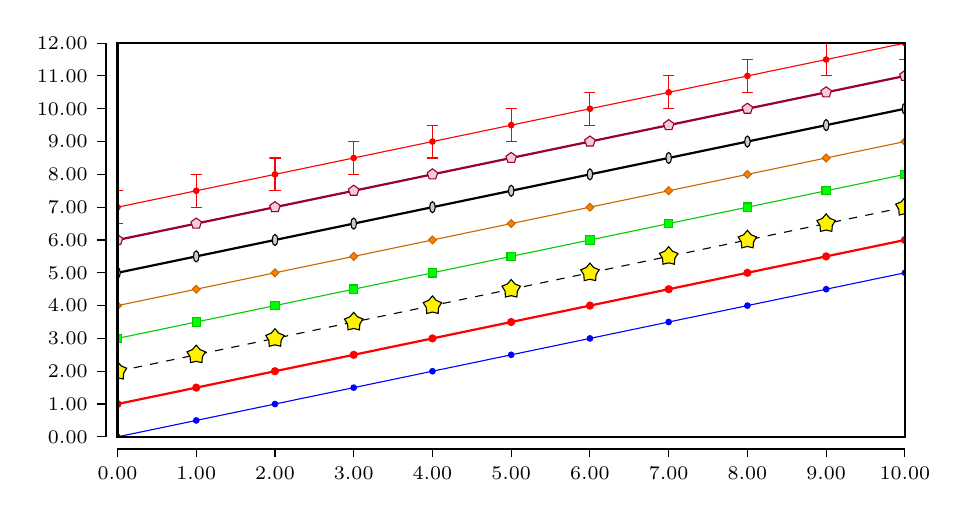
\begin{tikzpicture}[]
\begin{scope}[]
\clip (0,0) rectangle (10,5);
\begin{scope}[shift={(0.0,0.0)}]
\pgfsetxvec{\pgfpoint{1.0cm}{0cm}}
\pgfsetyvec{\pgfpoint{0cm}{0.41666666cm}}
\begin{scope}[blue]
\pgfpathmoveto{ \pgfqpointxy {0.0} {0.0}}
\pgfpathlineto{ \pgfqpointxy {1.0} {0.5}}
\pgfpathlineto{ \pgfqpointxy {2.0} {1.0}}
\pgfpathlineto{ \pgfqpointxy {3.0} {1.5}}
\pgfpathlineto{ \pgfqpointxy {4.0} {2.0}}
\pgfpathlineto{ \pgfqpointxy {5.0} {2.5}}
\pgfpathlineto{ \pgfqpointxy {6.0} {3.0}}
\pgfpathlineto{ \pgfqpointxy {7.0} {3.5}}
\pgfpathlineto{ \pgfqpointxy {8.0} {4.0}}
\pgfpathlineto{ \pgfqpointxy {9.0} {4.5}}
\pgfpathlineto{ \pgfqpointxy {10.0} {5.0}}
\pgfusepath{ stroke }
\end{scope}
\node at (0.0,0.0) [circle,inner sep=0pt,minimum width =2pt,minimum height=2pt,fill=blue,draw=blue] {}; 
\node at (1.0,0.5) [circle,inner sep=0pt,minimum width =2pt,minimum height=2pt,fill=blue,draw=blue] {}; 
\node at (2.0,1.0) [circle,inner sep=0pt,minimum width =2pt,minimum height=2pt,fill=blue,draw=blue] {}; 
\node at (3.0,1.5) [circle,inner sep=0pt,minimum width =2pt,minimum height=2pt,fill=blue,draw=blue] {}; 
\node at (4.0,2.0) [circle,inner sep=0pt,minimum width =2pt,minimum height=2pt,fill=blue,draw=blue] {}; 
\node at (5.0,2.5) [circle,inner sep=0pt,minimum width =2pt,minimum height=2pt,fill=blue,draw=blue] {}; 
\node at (6.0,3.0) [circle,inner sep=0pt,minimum width =2pt,minimum height=2pt,fill=blue,draw=blue] {}; 
\node at (7.0,3.5) [circle,inner sep=0pt,minimum width =2pt,minimum height=2pt,fill=blue,draw=blue] {}; 
\node at (8.0,4.0) [circle,inner sep=0pt,minimum width =2pt,minimum height=2pt,fill=blue,draw=blue] {}; 
\node at (9.0,4.5) [circle,inner sep=0pt,minimum width =2pt,minimum height=2pt,fill=blue,draw=blue] {}; 
\node at (10.0,5.0) [circle,inner sep=0pt,minimum width =2pt,minimum height=2pt,fill=blue,draw=blue] {}; 
\begin{scope}[red,thick]
\pgfpathmoveto{ \pgfqpointxy {0.0} {1.0}}
\pgfpathlineto{ \pgfqpointxy {1.0} {1.5}}
\pgfpathlineto{ \pgfqpointxy {2.0} {2.0}}
\pgfpathlineto{ \pgfqpointxy {3.0} {2.5}}
\pgfpathlineto{ \pgfqpointxy {4.0} {3.0}}
\pgfpathlineto{ \pgfqpointxy {5.0} {3.5}}
\pgfpathlineto{ \pgfqpointxy {6.0} {4.0}}
\pgfpathlineto{ \pgfqpointxy {7.0} {4.5}}
\pgfpathlineto{ \pgfqpointxy {8.0} {5.0}}
\pgfpathlineto{ \pgfqpointxy {9.0} {5.5}}
\pgfpathlineto{ \pgfqpointxy {10.0} {6.0}}
\pgfusepath{ stroke }
\end{scope}
\node at (0.0,1.0) [circle,inner sep=0pt,minimum width =3pt,minimum height=3pt,fill=red] {}; 
\node at (1.0,1.5) [circle,inner sep=0pt,minimum width =3pt,minimum height=3pt,fill=red] {}; 
\node at (2.0,2.0) [circle,inner sep=0pt,minimum width =3pt,minimum height=3pt,fill=red] {}; 
\node at (3.0,2.5) [circle,inner sep=0pt,minimum width =3pt,minimum height=3pt,fill=red] {}; 
\node at (4.0,3.0) [circle,inner sep=0pt,minimum width =3pt,minimum height=3pt,fill=red] {}; 
\node at (5.0,3.5) [circle,inner sep=0pt,minimum width =3pt,minimum height=3pt,fill=red] {}; 
\node at (6.0,4.0) [circle,inner sep=0pt,minimum width =3pt,minimum height=3pt,fill=red] {}; 
\node at (7.0,4.5) [circle,inner sep=0pt,minimum width =3pt,minimum height=3pt,fill=red] {}; 
\node at (8.0,5.0) [circle,inner sep=0pt,minimum width =3pt,minimum height=3pt,fill=red] {}; 
\node at (9.0,5.5) [circle,inner sep=0pt,minimum width =3pt,minimum height=3pt,fill=red] {}; 
\node at (10.0,6.0) [circle,inner sep=0pt,minimum width =3pt,minimum height=3pt,fill=red] {}; 
\begin{scope}[black,dashed]
\pgfpathmoveto{ \pgfqpointxy {0.0} {2.0}}
\pgfpathlineto{ \pgfqpointxy {1.0} {2.5}}
\pgfpathlineto{ \pgfqpointxy {2.0} {3.0}}
\pgfpathlineto{ \pgfqpointxy {3.0} {3.5}}
\pgfpathlineto{ \pgfqpointxy {4.0} {4.0}}
\pgfpathlineto{ \pgfqpointxy {5.0} {4.5}}
\pgfpathlineto{ \pgfqpointxy {6.0} {5.0}}
\pgfpathlineto{ \pgfqpointxy {7.0} {5.5}}
\pgfpathlineto{ \pgfqpointxy {8.0} {6.0}}
\pgfpathlineto{ \pgfqpointxy {9.0} {6.5}}
\pgfpathlineto{ \pgfqpointxy {10.0} {7.0}}
\pgfusepath{ stroke }
\end{scope}
\node at (0.0,2.0) [star,star points=5,inner sep=0pt,minimum width =7pt,minimum height=7pt,draw=black,fill=yellow] {}; 
\node at (1.0,2.5) [star,star points=5,inner sep=0pt,minimum width =7pt,minimum height=7pt,draw=black,fill=yellow] {}; 
\node at (2.0,3.0) [star,star points=5,inner sep=0pt,minimum width =7pt,minimum height=7pt,draw=black,fill=yellow] {}; 
\node at (3.0,3.5) [star,star points=5,inner sep=0pt,minimum width =7pt,minimum height=7pt,draw=black,fill=yellow] {}; 
\node at (4.0,4.0) [star,star points=5,inner sep=0pt,minimum width =7pt,minimum height=7pt,draw=black,fill=yellow] {}; 
\node at (5.0,4.5) [star,star points=5,inner sep=0pt,minimum width =7pt,minimum height=7pt,draw=black,fill=yellow] {}; 
\node at (6.0,5.0) [star,star points=5,inner sep=0pt,minimum width =7pt,minimum height=7pt,draw=black,fill=yellow] {}; 
\node at (7.0,5.5) [star,star points=5,inner sep=0pt,minimum width =7pt,minimum height=7pt,draw=black,fill=yellow] {}; 
\node at (8.0,6.0) [star,star points=5,inner sep=0pt,minimum width =7pt,minimum height=7pt,draw=black,fill=yellow] {}; 
\node at (9.0,6.5) [star,star points=5,inner sep=0pt,minimum width =7pt,minimum height=7pt,draw=black,fill=yellow] {}; 
\node at (10.0,7.0) [star,star points=5,inner sep=0pt,minimum width =7pt,minimum height=7pt,draw=black,fill=yellow] {}; 
\begin{scope}[green!80!black]
\pgfpathmoveto{ \pgfqpointxy {0.0} {3.0}}
\pgfpathlineto{ \pgfqpointxy {1.0} {3.5}}
\pgfpathlineto{ \pgfqpointxy {2.0} {4.0}}
\pgfpathlineto{ \pgfqpointxy {3.0} {4.5}}
\pgfpathlineto{ \pgfqpointxy {4.0} {5.0}}
\pgfpathlineto{ \pgfqpointxy {5.0} {5.5}}
\pgfpathlineto{ \pgfqpointxy {6.0} {6.0}}
\pgfpathlineto{ \pgfqpointxy {7.0} {6.5}}
\pgfpathlineto{ \pgfqpointxy {8.0} {7.0}}
\pgfpathlineto{ \pgfqpointxy {9.0} {7.5}}
\pgfpathlineto{ \pgfqpointxy {10.0} {8.0}}
\pgfusepath{ stroke }
\end{scope}
\node at (0.0,3.0) [rectangle,inner sep=0pt,minimum width =3pt,minimum height=3pt,draw=green!80!black,fill=green] {}; 
\node at (1.0,3.5) [rectangle,inner sep=0pt,minimum width =3pt,minimum height=3pt,draw=green!80!black,fill=green] {}; 
\node at (2.0,4.0) [rectangle,inner sep=0pt,minimum width =3pt,minimum height=3pt,draw=green!80!black,fill=green] {}; 
\node at (3.0,4.5) [rectangle,inner sep=0pt,minimum width =3pt,minimum height=3pt,draw=green!80!black,fill=green] {}; 
\node at (4.0,5.0) [rectangle,inner sep=0pt,minimum width =3pt,minimum height=3pt,draw=green!80!black,fill=green] {}; 
\node at (5.0,5.5) [rectangle,inner sep=0pt,minimum width =3pt,minimum height=3pt,draw=green!80!black,fill=green] {}; 
\node at (6.0,6.0) [rectangle,inner sep=0pt,minimum width =3pt,minimum height=3pt,draw=green!80!black,fill=green] {}; 
\node at (7.0,6.5) [rectangle,inner sep=0pt,minimum width =3pt,minimum height=3pt,draw=green!80!black,fill=green] {}; 
\node at (8.0,7.0) [rectangle,inner sep=0pt,minimum width =3pt,minimum height=3pt,draw=green!80!black,fill=green] {}; 
\node at (9.0,7.5) [rectangle,inner sep=0pt,minimum width =3pt,minimum height=3pt,draw=green!80!black,fill=green] {}; 
\node at (10.0,8.0) [rectangle,inner sep=0pt,minimum width =3pt,minimum height=3pt,draw=green!80!black,fill=green] {}; 
\begin{scope}[orange!80!black]
\pgfpathmoveto{ \pgfqpointxy {0.0} {4.0}}
\pgfpathlineto{ \pgfqpointxy {1.0} {4.5}}
\pgfpathlineto{ \pgfqpointxy {2.0} {5.0}}
\pgfpathlineto{ \pgfqpointxy {3.0} {5.5}}
\pgfpathlineto{ \pgfqpointxy {4.0} {6.0}}
\pgfpathlineto{ \pgfqpointxy {5.0} {6.5}}
\pgfpathlineto{ \pgfqpointxy {6.0} {7.0}}
\pgfpathlineto{ \pgfqpointxy {7.0} {7.5}}
\pgfpathlineto{ \pgfqpointxy {8.0} {8.0}}
\pgfpathlineto{ \pgfqpointxy {9.0} {8.5}}
\pgfpathlineto{ \pgfqpointxy {10.0} {9.0}}
\pgfusepath{ stroke }
\end{scope}
\node at (0.0,4.0) [diamond,inner sep=0pt,minimum width =3pt,minimum height=3pt,draw=orange!80!black,fill=orange] {}; 
\node at (1.0,4.5) [diamond,inner sep=0pt,minimum width =3pt,minimum height=3pt,draw=orange!80!black,fill=orange] {}; 
\node at (2.0,5.0) [diamond,inner sep=0pt,minimum width =3pt,minimum height=3pt,draw=orange!80!black,fill=orange] {}; 
\node at (3.0,5.5) [diamond,inner sep=0pt,minimum width =3pt,minimum height=3pt,draw=orange!80!black,fill=orange] {}; 
\node at (4.0,6.0) [diamond,inner sep=0pt,minimum width =3pt,minimum height=3pt,draw=orange!80!black,fill=orange] {}; 
\node at (5.0,6.5) [diamond,inner sep=0pt,minimum width =3pt,minimum height=3pt,draw=orange!80!black,fill=orange] {}; 
\node at (6.0,7.0) [diamond,inner sep=0pt,minimum width =3pt,minimum height=3pt,draw=orange!80!black,fill=orange] {}; 
\node at (7.0,7.5) [diamond,inner sep=0pt,minimum width =3pt,minimum height=3pt,draw=orange!80!black,fill=orange] {}; 
\node at (8.0,8.0) [diamond,inner sep=0pt,minimum width =3pt,minimum height=3pt,draw=orange!80!black,fill=orange] {}; 
\node at (9.0,8.5) [diamond,inner sep=0pt,minimum width =3pt,minimum height=3pt,draw=orange!80!black,fill=orange] {}; 
\node at (10.0,9.0) [diamond,inner sep=0pt,minimum width =3pt,minimum height=3pt,draw=orange!80!black,fill=orange] {}; 
\begin{scope}[black,thick]
\pgfpathmoveto{ \pgfqpointxy {0.0} {5.0}}
\pgfpathlineto{ \pgfqpointxy {1.0} {5.5}}
\pgfpathlineto{ \pgfqpointxy {2.0} {6.0}}
\pgfpathlineto{ \pgfqpointxy {3.0} {6.5}}
\pgfpathlineto{ \pgfqpointxy {4.0} {7.0}}
\pgfpathlineto{ \pgfqpointxy {5.0} {7.5}}
\pgfpathlineto{ \pgfqpointxy {6.0} {8.0}}
\pgfpathlineto{ \pgfqpointxy {7.0} {8.5}}
\pgfpathlineto{ \pgfqpointxy {8.0} {9.0}}
\pgfpathlineto{ \pgfqpointxy {9.0} {9.5}}
\pgfpathlineto{ \pgfqpointxy {10.0} {10.0}}
\pgfusepath{ stroke }
\end{scope}
\node at (0.0,5.0) [ellipse,inner sep=0pt,minimum width =2pt,minimum height=4pt,draw=black,fill=black!20] {}; 
\node at (1.0,5.5) [ellipse,inner sep=0pt,minimum width =2pt,minimum height=4pt,draw=black,fill=black!20] {}; 
\node at (2.0,6.0) [ellipse,inner sep=0pt,minimum width =2pt,minimum height=4pt,draw=black,fill=black!20] {}; 
\node at (3.0,6.5) [ellipse,inner sep=0pt,minimum width =2pt,minimum height=4pt,draw=black,fill=black!20] {}; 
\node at (4.0,7.0) [ellipse,inner sep=0pt,minimum width =2pt,minimum height=4pt,draw=black,fill=black!20] {}; 
\node at (5.0,7.5) [ellipse,inner sep=0pt,minimum width =2pt,minimum height=4pt,draw=black,fill=black!20] {}; 
\node at (6.0,8.0) [ellipse,inner sep=0pt,minimum width =2pt,minimum height=4pt,draw=black,fill=black!20] {}; 
\node at (7.0,8.5) [ellipse,inner sep=0pt,minimum width =2pt,minimum height=4pt,draw=black,fill=black!20] {}; 
\node at (8.0,9.0) [ellipse,inner sep=0pt,minimum width =2pt,minimum height=4pt,draw=black,fill=black!20] {}; 
\node at (9.0,9.5) [ellipse,inner sep=0pt,minimum width =2pt,minimum height=4pt,draw=black,fill=black!20] {}; 
\node at (10.0,10.0) [ellipse,inner sep=0pt,minimum width =2pt,minimum height=4pt,draw=black,fill=black!20] {}; 
\begin{scope}[purple!80!black,thick]
\pgfpathmoveto{ \pgfqpointxy {0.0} {6.0}}
\pgfpathlineto{ \pgfqpointxy {1.0} {6.5}}
\pgfpathlineto{ \pgfqpointxy {2.0} {7.0}}
\pgfpathlineto{ \pgfqpointxy {3.0} {7.5}}
\pgfpathlineto{ \pgfqpointxy {4.0} {8.0}}
\pgfpathlineto{ \pgfqpointxy {5.0} {8.5}}
\pgfpathlineto{ \pgfqpointxy {6.0} {9.0}}
\pgfpathlineto{ \pgfqpointxy {7.0} {9.5}}
\pgfpathlineto{ \pgfqpointxy {8.0} {10.0}}
\pgfpathlineto{ \pgfqpointxy {9.0} {10.5}}
\pgfpathlineto{ \pgfqpointxy {10.0} {11.0}}
\pgfusepath{ stroke }
\end{scope}
\node at (0.0,6.0) [regular polygon,regular polygon sides=5,inner sep=0pt,minimum width =4pt,minimum height=4pt,draw=purple!80!black,fill=purple!20] {}; 
\node at (1.0,6.5) [regular polygon,regular polygon sides=5,inner sep=0pt,minimum width =4pt,minimum height=4pt,draw=purple!80!black,fill=purple!20] {}; 
\node at (2.0,7.0) [regular polygon,regular polygon sides=5,inner sep=0pt,minimum width =4pt,minimum height=4pt,draw=purple!80!black,fill=purple!20] {}; 
\node at (3.0,7.5) [regular polygon,regular polygon sides=5,inner sep=0pt,minimum width =4pt,minimum height=4pt,draw=purple!80!black,fill=purple!20] {}; 
\node at (4.0,8.0) [regular polygon,regular polygon sides=5,inner sep=0pt,minimum width =4pt,minimum height=4pt,draw=purple!80!black,fill=purple!20] {}; 
\node at (5.0,8.5) [regular polygon,regular polygon sides=5,inner sep=0pt,minimum width =4pt,minimum height=4pt,draw=purple!80!black,fill=purple!20] {}; 
\node at (6.0,9.0) [regular polygon,regular polygon sides=5,inner sep=0pt,minimum width =4pt,minimum height=4pt,draw=purple!80!black,fill=purple!20] {}; 
\node at (7.0,9.5) [regular polygon,regular polygon sides=5,inner sep=0pt,minimum width =4pt,minimum height=4pt,draw=purple!80!black,fill=purple!20] {}; 
\node at (8.0,10.0) [regular polygon,regular polygon sides=5,inner sep=0pt,minimum width =4pt,minimum height=4pt,draw=purple!80!black,fill=purple!20] {}; 
\node at (9.0,10.5) [regular polygon,regular polygon sides=5,inner sep=0pt,minimum width =4pt,minimum height=4pt,draw=purple!80!black,fill=purple!20] {}; 
\node at (10.0,11.0) [regular polygon,regular polygon sides=5,inner sep=0pt,minimum width =4pt,minimum height=4pt,draw=purple!80!black,fill=purple!20] {}; 
\begin{scope}[red]
\pgfpathmoveto{ \pgfqpointxy {0.0} {7.0}}
\pgfpathlineto{ \pgfqpointxy {1.0} {7.5}}
\pgfpathlineto{ \pgfqpointxy {2.0} {8.0}}
\pgfpathlineto{ \pgfqpointxy {3.0} {8.5}}
\pgfpathlineto{ \pgfqpointxy {4.0} {9.0}}
\pgfpathlineto{ \pgfqpointxy {5.0} {9.5}}
\pgfpathlineto{ \pgfqpointxy {6.0} {10.0}}
\pgfpathlineto{ \pgfqpointxy {7.0} {10.5}}
\pgfpathlineto{ \pgfqpointxy {8.0} {11.0}}
\pgfpathlineto{ \pgfqpointxy {9.0} {11.5}}
\pgfpathlineto{ \pgfqpointxy {10.0} {12.0}}
\pgfusepath{ stroke }
\end{scope}
\begin{scope}[draw=red,fill=red]
\pgfpathmoveto{ \pgfqpointxy {0.0} {6.5}}
\pgfpathlineto{ \pgfqpointxy {0.0} {7.5}}
\pgfusepath{ stroke }
\end{scope}
\node at (0.0,7.0) [circle,inner sep=0pt,minimum width =2pt,minimum height=2pt,draw=red,fill=red] {}; 
\begin{scope}[draw=red,fill=red]
\pgfpathmoveto{ \pgfpointadd{\pgfqpointxy {0.0} {7.5}} {\pgfpoint{2pt}{0}}}
\pgfpathlineto{ \pgfpointadd{\pgfqpointxy {0.0} {7.5}} {\pgfpoint{-2pt}{0}}}
\pgfpathlineto{ \pgfqpointxy {0.0} {7.5}}
\pgfpathlineto{ \pgfqpointxy {0.0} {6.5}}
\pgfpathmoveto{ \pgfpointadd{\pgfqpointxy {0.0} {6.5}} {\pgfpoint {2pt} {0} }}
\pgfpathlineto{ \pgfpointadd{\pgfqpointxy {0.0} {6.5}} {\pgfpoint {-2pt} {0} }}
\pgfusepath{ stroke }
\end{scope}
\begin{scope}[draw=red,fill=red]
\pgfpathmoveto{ \pgfqpointxy {1.0} {7.0}}
\pgfpathlineto{ \pgfqpointxy {1.0} {8.0}}
\pgfusepath{ stroke }
\end{scope}
\node at (1.0,7.5) [circle,inner sep=0pt,minimum width =2pt,minimum height=2pt,draw=red,fill=red] {}; 
\begin{scope}[draw=red,fill=red]
\pgfpathmoveto{ \pgfpointadd{\pgfqpointxy {1.0} {8.0}} {\pgfpoint{2pt}{0}}}
\pgfpathlineto{ \pgfpointadd{\pgfqpointxy {1.0} {8.0}} {\pgfpoint{-2pt}{0}}}
\pgfpathlineto{ \pgfqpointxy {1.0} {8.0}}
\pgfpathlineto{ \pgfqpointxy {1.0} {7.0}}
\pgfpathmoveto{ \pgfpointadd{\pgfqpointxy {1.0} {7.0}} {\pgfpoint {2pt} {0} }}
\pgfpathlineto{ \pgfpointadd{\pgfqpointxy {1.0} {7.0}} {\pgfpoint {-2pt} {0} }}
\pgfusepath{ stroke }
\end{scope}
\begin{scope}[draw=red,fill=red]
\pgfpathmoveto{ \pgfqpointxy {2.0} {7.5}}
\pgfpathlineto{ \pgfqpointxy {2.0} {8.5}}
\pgfusepath{ stroke }
\end{scope}
\node at (2.0,8.0) [circle,inner sep=0pt,minimum width =2pt,minimum height=2pt,draw=red,fill=red] {}; 
\begin{scope}[draw=red,fill=red]
\pgfpathmoveto{ \pgfpointadd{\pgfqpointxy {2.0} {8.5}} {\pgfpoint{2pt}{0}}}
\pgfpathlineto{ \pgfpointadd{\pgfqpointxy {2.0} {8.5}} {\pgfpoint{-2pt}{0}}}
\pgfpathlineto{ \pgfqpointxy {2.0} {8.5}}
\pgfpathlineto{ \pgfqpointxy {2.0} {7.5}}
\pgfpathmoveto{ \pgfpointadd{\pgfqpointxy {2.0} {7.5}} {\pgfpoint {2pt} {0} }}
\pgfpathlineto{ \pgfpointadd{\pgfqpointxy {2.0} {7.5}} {\pgfpoint {-2pt} {0} }}
\pgfusepath{ stroke }
\end{scope}
\begin{scope}[draw=red,fill=red]
\pgfpathmoveto{ \pgfqpointxy {3.0} {8.0}}
\pgfpathlineto{ \pgfqpointxy {3.0} {9.0}}
\pgfusepath{ stroke }
\end{scope}
\node at (3.0,8.5) [circle,inner sep=0pt,minimum width =2pt,minimum height=2pt,draw=red,fill=red] {}; 
\begin{scope}[draw=red,fill=red]
\pgfpathmoveto{ \pgfpointadd{\pgfqpointxy {3.0} {9.0}} {\pgfpoint{2pt}{0}}}
\pgfpathlineto{ \pgfpointadd{\pgfqpointxy {3.0} {9.0}} {\pgfpoint{-2pt}{0}}}
\pgfpathlineto{ \pgfqpointxy {3.0} {9.0}}
\pgfpathlineto{ \pgfqpointxy {3.0} {8.0}}
\pgfpathmoveto{ \pgfpointadd{\pgfqpointxy {3.0} {8.0}} {\pgfpoint {2pt} {0} }}
\pgfpathlineto{ \pgfpointadd{\pgfqpointxy {3.0} {8.0}} {\pgfpoint {-2pt} {0} }}
\pgfusepath{ stroke }
\end{scope}
\begin{scope}[draw=red,fill=red]
\pgfpathmoveto{ \pgfqpointxy {4.0} {8.5}}
\pgfpathlineto{ \pgfqpointxy {4.0} {9.5}}
\pgfusepath{ stroke }
\end{scope}
\node at (4.0,9.0) [circle,inner sep=0pt,minimum width =2pt,minimum height=2pt,draw=red,fill=red] {}; 
\begin{scope}[draw=red,fill=red]
\pgfpathmoveto{ \pgfpointadd{\pgfqpointxy {4.0} {9.5}} {\pgfpoint{2pt}{0}}}
\pgfpathlineto{ \pgfpointadd{\pgfqpointxy {4.0} {9.5}} {\pgfpoint{-2pt}{0}}}
\pgfpathlineto{ \pgfqpointxy {4.0} {9.5}}
\pgfpathlineto{ \pgfqpointxy {4.0} {8.5}}
\pgfpathmoveto{ \pgfpointadd{\pgfqpointxy {4.0} {8.5}} {\pgfpoint {2pt} {0} }}
\pgfpathlineto{ \pgfpointadd{\pgfqpointxy {4.0} {8.5}} {\pgfpoint {-2pt} {0} }}
\pgfusepath{ stroke }
\end{scope}
\begin{scope}[draw=red,fill=red]
\pgfpathmoveto{ \pgfqpointxy {5.0} {9.0}}
\pgfpathlineto{ \pgfqpointxy {5.0} {10.0}}
\pgfusepath{ stroke }
\end{scope}
\node at (5.0,9.5) [circle,inner sep=0pt,minimum width =2pt,minimum height=2pt,draw=red,fill=red] {}; 
\begin{scope}[draw=red,fill=red]
\pgfpathmoveto{ \pgfpointadd{\pgfqpointxy {5.0} {10.0}} {\pgfpoint{2pt}{0}}}
\pgfpathlineto{ \pgfpointadd{\pgfqpointxy {5.0} {10.0}} {\pgfpoint{-2pt}{0}}}
\pgfpathlineto{ \pgfqpointxy {5.0} {10.0}}
\pgfpathlineto{ \pgfqpointxy {5.0} {9.0}}
\pgfpathmoveto{ \pgfpointadd{\pgfqpointxy {5.0} {9.0}} {\pgfpoint {2pt} {0} }}
\pgfpathlineto{ \pgfpointadd{\pgfqpointxy {5.0} {9.0}} {\pgfpoint {-2pt} {0} }}
\pgfusepath{ stroke }
\end{scope}
\begin{scope}[draw=red,fill=red]
\pgfpathmoveto{ \pgfqpointxy {6.0} {9.5}}
\pgfpathlineto{ \pgfqpointxy {6.0} {10.5}}
\pgfusepath{ stroke }
\end{scope}
\node at (6.0,10.0) [circle,inner sep=0pt,minimum width =2pt,minimum height=2pt,draw=red,fill=red] {}; 
\begin{scope}[draw=red,fill=red]
\pgfpathmoveto{ \pgfpointadd{\pgfqpointxy {6.0} {10.5}} {\pgfpoint{2pt}{0}}}
\pgfpathlineto{ \pgfpointadd{\pgfqpointxy {6.0} {10.5}} {\pgfpoint{-2pt}{0}}}
\pgfpathlineto{ \pgfqpointxy {6.0} {10.5}}
\pgfpathlineto{ \pgfqpointxy {6.0} {9.5}}
\pgfpathmoveto{ \pgfpointadd{\pgfqpointxy {6.0} {9.5}} {\pgfpoint {2pt} {0} }}
\pgfpathlineto{ \pgfpointadd{\pgfqpointxy {6.0} {9.5}} {\pgfpoint {-2pt} {0} }}
\pgfusepath{ stroke }
\end{scope}
\begin{scope}[draw=red,fill=red]
\pgfpathmoveto{ \pgfqpointxy {7.0} {10.0}}
\pgfpathlineto{ \pgfqpointxy {7.0} {11.0}}
\pgfusepath{ stroke }
\end{scope}
\node at (7.0,10.5) [circle,inner sep=0pt,minimum width =2pt,minimum height=2pt,draw=red,fill=red] {}; 
\begin{scope}[draw=red,fill=red]
\pgfpathmoveto{ \pgfpointadd{\pgfqpointxy {7.0} {11.0}} {\pgfpoint{2pt}{0}}}
\pgfpathlineto{ \pgfpointadd{\pgfqpointxy {7.0} {11.0}} {\pgfpoint{-2pt}{0}}}
\pgfpathlineto{ \pgfqpointxy {7.0} {11.0}}
\pgfpathlineto{ \pgfqpointxy {7.0} {10.0}}
\pgfpathmoveto{ \pgfpointadd{\pgfqpointxy {7.0} {10.0}} {\pgfpoint {2pt} {0} }}
\pgfpathlineto{ \pgfpointadd{\pgfqpointxy {7.0} {10.0}} {\pgfpoint {-2pt} {0} }}
\pgfusepath{ stroke }
\end{scope}
\begin{scope}[draw=red,fill=red]
\pgfpathmoveto{ \pgfqpointxy {8.0} {10.5}}
\pgfpathlineto{ \pgfqpointxy {8.0} {11.5}}
\pgfusepath{ stroke }
\end{scope}
\node at (8.0,11.0) [circle,inner sep=0pt,minimum width =2pt,minimum height=2pt,draw=red,fill=red] {}; 
\begin{scope}[draw=red,fill=red]
\pgfpathmoveto{ \pgfpointadd{\pgfqpointxy {8.0} {11.5}} {\pgfpoint{2pt}{0}}}
\pgfpathlineto{ \pgfpointadd{\pgfqpointxy {8.0} {11.5}} {\pgfpoint{-2pt}{0}}}
\pgfpathlineto{ \pgfqpointxy {8.0} {11.5}}
\pgfpathlineto{ \pgfqpointxy {8.0} {10.5}}
\pgfpathmoveto{ \pgfpointadd{\pgfqpointxy {8.0} {10.5}} {\pgfpoint {2pt} {0} }}
\pgfpathlineto{ \pgfpointadd{\pgfqpointxy {8.0} {10.5}} {\pgfpoint {-2pt} {0} }}
\pgfusepath{ stroke }
\end{scope}
\begin{scope}[draw=red,fill=red]
\pgfpathmoveto{ \pgfqpointxy {9.0} {11.0}}
\pgfpathlineto{ \pgfqpointxy {9.0} {12.0}}
\pgfusepath{ stroke }
\end{scope}
\node at (9.0,11.5) [circle,inner sep=0pt,minimum width =2pt,minimum height=2pt,draw=red,fill=red] {}; 
\begin{scope}[draw=red,fill=red]
\pgfpathmoveto{ \pgfpointadd{\pgfqpointxy {9.0} {12.0}} {\pgfpoint{2pt}{0}}}
\pgfpathlineto{ \pgfpointadd{\pgfqpointxy {9.0} {12.0}} {\pgfpoint{-2pt}{0}}}
\pgfpathlineto{ \pgfqpointxy {9.0} {12.0}}
\pgfpathlineto{ \pgfqpointxy {9.0} {11.0}}
\pgfpathmoveto{ \pgfpointadd{\pgfqpointxy {9.0} {11.0}} {\pgfpoint {2pt} {0} }}
\pgfpathlineto{ \pgfpointadd{\pgfqpointxy {9.0} {11.0}} {\pgfpoint {-2pt} {0} }}
\pgfusepath{ stroke }
\end{scope}
\begin{scope}[draw=red,fill=red]
\pgfpathmoveto{ \pgfqpointxy {10.0} {11.5}}
\pgfpathlineto{ \pgfqpointxy {10.0} {12.5}}
\pgfusepath{ stroke }
\end{scope}
\node at (10.0,12.0) [circle,inner sep=0pt,minimum width =2pt,minimum height=2pt,draw=red,fill=red] {}; 
\begin{scope}[draw=red,fill=red]
\pgfpathmoveto{ \pgfpointadd{\pgfqpointxy {10.0} {12.5}} {\pgfpoint{2pt}{0}}}
\pgfpathlineto{ \pgfpointadd{\pgfqpointxy {10.0} {12.5}} {\pgfpoint{-2pt}{0}}}
\pgfpathlineto{ \pgfqpointxy {10.0} {12.5}}
\pgfpathlineto{ \pgfqpointxy {10.0} {11.5}}
\pgfpathmoveto{ \pgfpointadd{\pgfqpointxy {10.0} {11.5}} {\pgfpoint {2pt} {0} }}
\pgfpathlineto{ \pgfpointadd{\pgfqpointxy {10.0} {11.5}} {\pgfpoint {-2pt} {0} }}
\pgfusepath{ stroke }
\end{scope}
\pgfsetxvec{\pgfpoint{1cm}{0cm}}
\pgfsetyvec{\pgfpoint{0cm}{1cm}}
\end{scope}
\end{scope}
\begin{scope}[shift={(0.0,0.0)}]
\pgfsetxvec{\pgfpoint{1.0cm}{0cm}}
\pgfsetyvec{\pgfpoint{0cm}{0.41666666cm}}
\begin{scope}[yshift=-0.15cm]
\draw[] [shift={(0.0,0.0)}] (0pt,0pt) -- (-0pt,-3pt) node[below]{ \scriptsize{\num[round-mode=places,round-precision=2]{0}}};
\draw[] [shift={(1.0,0.0)}] (0pt,0pt) -- (-0pt,-3pt) node[below]{ \scriptsize{\num[round-mode=places,round-precision=2]{1}}};
\draw[] [shift={(2.0,0.0)}] (0pt,0pt) -- (-0pt,-3pt) node[below]{ \scriptsize{\num[round-mode=places,round-precision=2]{2}}};
\draw[] [shift={(3.0,0.0)}] (0pt,0pt) -- (-0pt,-3pt) node[below]{ \scriptsize{\num[round-mode=places,round-precision=2]{3}}};
\draw[] [shift={(4.0,0.0)}] (0pt,0pt) -- (-0pt,-3pt) node[below]{ \scriptsize{\num[round-mode=places,round-precision=2]{4}}};
\draw[] [shift={(5.0,0.0)}] (0pt,0pt) -- (-0pt,-3pt) node[below]{ \scriptsize{\num[round-mode=places,round-precision=2]{5}}};
\draw[] [shift={(6.0,0.0)}] (0pt,0pt) -- (-0pt,-3pt) node[below]{ \scriptsize{\num[round-mode=places,round-precision=2]{6}}};
\draw[] [shift={(7.0,0.0)}] (0pt,0pt) -- (-0pt,-3pt) node[below]{ \scriptsize{\num[round-mode=places,round-precision=2]{7}}};
\draw[] [shift={(8.0,0.0)}] (0pt,0pt) -- (-0pt,-3pt) node[below]{ \scriptsize{\num[round-mode=places,round-precision=2]{8}}};
\draw[] [shift={(9.0,0.0)}] (0pt,0pt) -- (-0pt,-3pt) node[below]{ \scriptsize{\num[round-mode=places,round-precision=2]{9}}};
\draw[] [shift={(10.0,0.0)}] (0pt,0pt) -- (-0pt,-3pt) node[below]{ \scriptsize{\num[round-mode=places,round-precision=2]{10}}};
\end{scope}
\begin{scope}[xshift=-0.15cm]
\draw[] [shift={(0.0,0.0)}] (0pt,0pt) -- (-3pt,-0pt) node[left]{ \scriptsize{\num[round-mode=places,round-precision=2]{0}}};
\draw[] [shift={(0.0,1.0)}] (0pt,0pt) -- (-3pt,-0pt) node[left]{ \scriptsize{\num[round-mode=places,round-precision=2]{1}}};
\draw[] [shift={(0.0,2.0)}] (0pt,0pt) -- (-3pt,-0pt) node[left]{ \scriptsize{\num[round-mode=places,round-precision=2]{2}}};
\draw[] [shift={(0.0,3.0)}] (0pt,0pt) -- (-3pt,-0pt) node[left]{ \scriptsize{\num[round-mode=places,round-precision=2]{3}}};
\draw[] [shift={(0.0,4.0)}] (0pt,0pt) -- (-3pt,-0pt) node[left]{ \scriptsize{\num[round-mode=places,round-precision=2]{4}}};
\draw[] [shift={(0.0,5.0)}] (0pt,0pt) -- (-3pt,-0pt) node[left]{ \scriptsize{\num[round-mode=places,round-precision=2]{5}}};
\draw[] [shift={(0.0,6.0)}] (0pt,0pt) -- (-3pt,-0pt) node[left]{ \scriptsize{\num[round-mode=places,round-precision=2]{6}}};
\draw[] [shift={(0.0,7.0)}] (0pt,0pt) -- (-3pt,-0pt) node[left]{ \scriptsize{\num[round-mode=places,round-precision=2]{7}}};
\draw[] [shift={(0.0,8.0)}] (0pt,0pt) -- (-3pt,-0pt) node[left]{ \scriptsize{\num[round-mode=places,round-precision=2]{8}}};
\draw[] [shift={(0.0,9.0)}] (0pt,0pt) -- (-3pt,-0pt) node[left]{ \scriptsize{\num[round-mode=places,round-precision=2]{9}}};
\draw[] [shift={(0.0,10.0)}] (0pt,0pt) -- (-3pt,-0pt) node[left]{ \scriptsize{\num[round-mode=places,round-precision=2]{10}}};
\draw[] [shift={(0.0,11.0)}] (0pt,0pt) -- (-3pt,-0pt) node[left]{ \scriptsize{\num[round-mode=places,round-precision=2]{11}}};
\draw[] [shift={(0.0,12.0)}] (0pt,0pt) -- (-3pt,-0pt) node[left]{ \scriptsize{\num[round-mode=places,round-precision=2]{12}}};
\end{scope}
\pgfsetxvec{\pgfpoint{1cm}{0cm}}
\pgfsetyvec{\pgfpoint{0cm}{1cm}}
\end{scope}
\draw[black,thick] (0.0,-0.15) -- (10.0,-0.15);
\draw[black,thick] (-0.15,0.0) -- (-0.15,5.0);
\draw[thick] (0,0) rectangle (10,5);
\end{tikzpicture}
%%% Local Variables: 
%%% mode: latex 
%%% TeX-master: "master" 
%%% End:


  \caption{Different line marker styles}
\end{figure}

\begin{figure}[H]
  \centering
  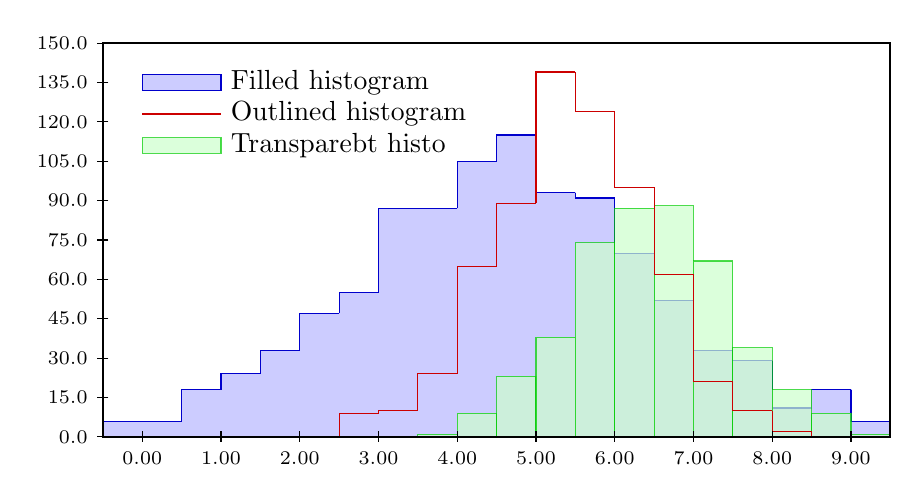
\begin{tikzpicture}
\begin{scope}[]
\clip (0,0) rectangle (10,5);
\begin{scope}[draw=blue!20,fill=blue!20]
\filldraw[] (0.0,0.0) -- (0.0,0.2) -- (0.5,0.2) -- (0.5,0.0);
\filldraw[] (0.5,0.0) -- (0.5,0.2) -- (1.0,0.2) -- (1.0,0.0);
\filldraw[] (1.0,0.0) -- (1.0,0.6) -- (1.5,0.6) -- (1.5,0.0);
\filldraw[] (1.5,0.0) -- (1.5,0.8) -- (2.0,0.8) -- (2.0,0.0);
\filldraw[] (2.0,0.0) -- (2.0,1.1) -- (2.5,1.1) -- (2.5,0.0);
\filldraw[] (2.5,0.0) -- (2.5,1.5666667) -- (3.0,1.5666667) -- (3.0,0.0);
\filldraw[] (3.0,0.0) -- (3.0,1.8333334) -- (3.5,1.8333334) -- (3.5,0.0);
\filldraw[] (3.5,0.0) -- (3.5,2.9) -- (4.0,2.9) -- (4.0,0.0);
\filldraw[] (4.0,0.0) -- (4.0,2.9) -- (4.5,2.9) -- (4.5,0.0);
\filldraw[] (4.5,0.0) -- (4.5,3.5) -- (5.0,3.5) -- (5.0,0.0);
\filldraw[] (5.0,0.0) -- (5.0,3.8333333) -- (5.5,3.8333333) -- (5.5,0.0);
\filldraw[] (5.5,0.0) -- (5.5,3.1) -- (6.0,3.1) -- (6.0,0.0);
\filldraw[] (6.0,0.0) -- (6.0,3.0333333) -- (6.5,3.0333333) -- (6.5,0.0);
\filldraw[] (6.5,0.0) -- (6.5,2.3333333) -- (7.0,2.3333333) -- (7.0,0.0);
\filldraw[] (7.0,0.0) -- (7.0,1.7333333) -- (7.5,1.7333333) -- (7.5,0.0);
\filldraw[] (7.5,0.0) -- (7.5,1.1) -- (8.0,1.1) -- (8.0,0.0);
\filldraw[] (8.0,0.0) -- (8.0,0.96666664) -- (8.5,0.96666664) -- (8.5,0.0);
\filldraw[] (8.5,0.0) -- (8.5,0.36666667) -- (9.0,0.36666667) -- (9.0,0.0);
\filldraw[] (9.0,0.0) -- (9.0,0.6) -- (9.5,0.6) -- (9.5,0.0);
\filldraw[] (9.5,0.0) -- (9.5,0.2) -- (10.0,0.2) -- (10.0,0.0);
\end{scope}
\begin{scope}[blue!80!black]
\draw[] (0.0,0.2) -- (0.5,0.2);
\draw (0.5,0.2) -- (0.5,0.2) -- (1.0,0.2);
\draw (1.0,0.2) -- (1.0,0.6) -- (1.5,0.6);
\draw (1.5,0.6) -- (1.5,0.8) -- (2.0,0.8);
\draw (2.0,0.8) -- (2.0,1.1) -- (2.5,1.1);
\draw (2.5,1.1) -- (2.5,1.5666667) -- (3.0,1.5666667);
\draw (3.0,1.5666667) -- (3.0,1.8333334) -- (3.5,1.8333334);
\draw (3.5,1.8333334) -- (3.5,2.9) -- (4.0,2.9);
\draw (4.0,2.9) -- (4.0,2.9) -- (4.5,2.9);
\draw (4.5,2.9) -- (4.5,3.5) -- (5.0,3.5);
\draw (5.0,3.5) -- (5.0,3.8333333) -- (5.5,3.8333333);
\draw (5.5,3.8333333) -- (5.5,3.1) -- (6.0,3.1);
\draw (6.0,3.1) -- (6.0,3.0333333) -- (6.5,3.0333333);
\draw (6.5,3.0333333) -- (6.5,2.3333333) -- (7.0,2.3333333);
\draw (7.0,2.3333333) -- (7.0,1.7333333) -- (7.5,1.7333333);
\draw (7.5,1.7333333) -- (7.5,1.1) -- (8.0,1.1);
\draw (8.0,1.1) -- (8.0,0.96666664) -- (8.5,0.96666664);
\draw (8.5,0.96666664) -- (8.5,0.36666667) -- (9.0,0.36666667);
\draw (9.0,0.36666667) -- (9.0,0.6) -- (9.5,0.6);
\draw (9.5,0.6) -- (9.5,0.2) -- (10.0,0.2);
\end{scope}
\begin{scope}[opacity=0.7,draw=green!80!black,fill=green!20]
\filldraw[] (0.0,0.0) -- (0.0,0.0) -- (0.5,0.0) -- (0.5,0.0);
\filldraw[] (0.5,0.0) -- (0.5,0.0) -- (1.0,0.0) -- (1.0,0.0);
\filldraw[] (1.0,0.0) -- (1.0,0.0) -- (1.5,0.0) -- (1.5,0.0);
\filldraw[] (1.5,0.0) -- (1.5,0.0) -- (2.0,0.0) -- (2.0,0.0);
\filldraw[] (2.0,0.0) -- (2.0,0.0) -- (2.5,0.0) -- (2.5,0.0);
\filldraw[] (2.5,0.0) -- (2.5,0.0) -- (3.0,0.0) -- (3.0,0.0);
\filldraw[] (3.0,0.0) -- (3.0,0.0) -- (3.5,0.0) -- (3.5,0.0);
\filldraw[] (3.5,0.0) -- (3.5,0.0) -- (4.0,0.0) -- (4.0,0.0);
\filldraw[] (4.0,0.0) -- (4.0,0.033333335) -- (4.5,0.033333335) -- (4.5,0.0);
\filldraw[] (4.5,0.0) -- (4.5,0.3) -- (5.0,0.3) -- (5.0,0.0);
\filldraw[] (5.0,0.0) -- (5.0,0.76666665) -- (5.5,0.76666665) -- (5.5,0.0);
\filldraw[] (5.5,0.0) -- (5.5,1.2666667) -- (6.0,1.2666667) -- (6.0,0.0);
\filldraw[] (6.0,0.0) -- (6.0,2.4666667) -- (6.5,2.4666667) -- (6.5,0.0);
\filldraw[] (6.5,0.0) -- (6.5,2.9) -- (7.0,2.9) -- (7.0,0.0);
\filldraw[] (7.0,0.0) -- (7.0,2.9333334) -- (7.5,2.9333334) -- (7.5,0.0);
\filldraw[] (7.5,0.0) -- (7.5,2.2333333) -- (8.0,2.2333333) -- (8.0,0.0);
\filldraw[] (8.0,0.0) -- (8.0,1.1333333) -- (8.5,1.1333333) -- (8.5,0.0);
\filldraw[] (8.5,0.0) -- (8.5,0.6) -- (9.0,0.6) -- (9.0,0.0);
\filldraw[] (9.0,0.0) -- (9.0,0.3) -- (9.5,0.3) -- (9.5,0.0);
\filldraw[] (9.5,0.0) -- (9.5,0.033333335) -- (10.0,0.033333335) -- (10.0,0.0);
\end{scope}
\begin{scope}[red!80!black]
\draw[] (0.0,0.0) -- (0.5,0.0);
\draw (0.5,0.0) -- (0.5,0.0) -- (1.0,0.0);
\draw (1.0,0.0) -- (1.0,0.0) -- (1.5,0.0);
\draw (1.5,0.0) -- (1.5,0.0) -- (2.0,0.0);
\draw (2.0,0.0) -- (2.0,0.0) -- (2.5,0.0);
\draw (2.5,0.0) -- (2.5,0.0) -- (3.0,0.0);
\draw (3.0,0.0) -- (3.0,0.3) -- (3.5,0.3);
\draw (3.5,0.3) -- (3.5,0.33333334) -- (4.0,0.33333334);
\draw (4.0,0.33333334) -- (4.0,0.8) -- (4.5,0.8);
\draw (4.5,0.8) -- (4.5,2.1666667) -- (5.0,2.1666667);
\draw (5.0,2.1666667) -- (5.0,2.9666667) -- (5.5,2.9666667);
\draw (5.5,2.9666667) -- (5.5,4.633333) -- (6.0,4.633333);
\draw (6.0,4.633333) -- (6.0,4.133333) -- (6.5,4.133333);
\draw (6.5,4.133333) -- (6.5,3.1666667) -- (7.0,3.1666667);
\draw (7.0,3.1666667) -- (7.0,2.0666666) -- (7.5,2.0666666);
\draw (7.5,2.0666666) -- (7.5,0.7) -- (8.0,0.7);
\draw (8.0,0.7) -- (8.0,0.33333334) -- (8.5,0.33333334);
\draw (8.5,0.33333334) -- (8.5,0.06666667) -- (9.0,0.06666667);
\draw (9.0,0.06666667) -- (9.0,0.0) -- (9.5,0.0);
\draw (9.5,0.0) -- (9.5,0.0) -- (10.0,0.0);
\end{scope}
\end{scope}
\draw (0.5,0cm + 2pt) -- (0.5, 0cm -2pt) node[below] {\scriptsize{\num[round-mode=places,round-precision=2]{0}}};
\draw (1.5,0cm + 2pt) -- (1.5, 0cm -2pt) node[below] {\scriptsize{\num[round-mode=places,round-precision=2]{1}}};
\draw (2.5,0cm + 2pt) -- (2.5, 0cm -2pt) node[below] {\scriptsize{\num[round-mode=places,round-precision=2]{2}}};
\draw (3.5,0cm + 2pt) -- (3.5, 0cm -2pt) node[below] {\scriptsize{\num[round-mode=places,round-precision=2]{3}}};
\draw (4.5,0cm + 2pt) -- (4.5, 0cm -2pt) node[below] {\scriptsize{\num[round-mode=places,round-precision=2]{4}}};
\draw (5.5,0cm + 2pt) -- (5.5, 0cm -2pt) node[below] {\scriptsize{\num[round-mode=places,round-precision=2]{5}}};
\draw (6.5,0cm + 2pt) -- (6.5, 0cm -2pt) node[below] {\scriptsize{\num[round-mode=places,round-precision=2]{6}}};
\draw (7.5,0cm + 2pt) -- (7.5, 0cm -2pt) node[below] {\scriptsize{\num[round-mode=places,round-precision=2]{7}}};
\draw (8.5,0cm + 2pt) -- (8.5, 0cm -2pt) node[below] {\scriptsize{\num[round-mode=places,round-precision=2]{8}}};
\draw (9.5,0cm + 2pt) -- (9.5, 0cm -2pt) node[below] {\scriptsize{\num[round-mode=places,round-precision=2]{9}}};
\draw (0cm + 2pt,0.    ) -- (0cm-2pt,0.    ) node[left] {\scriptsize{\num[round-mode=places,round-precision=1]{0}}};
\draw (0cm + 2pt,0.5    ) -- (0cm-2pt,0.5    ) node[left] {\scriptsize{\num[round-mode=places,round-precision=1]{15}}};
\draw (0cm + 2pt,1.    ) -- (0cm-2pt,1.    ) node[left] {\scriptsize{\num[round-mode=places,round-precision=1]{30}}};
\draw (0cm + 2pt,1.5    ) -- (0cm-2pt,1.5    ) node[left] {\scriptsize{\num[round-mode=places,round-precision=1]{45}}};
\draw (0cm + 2pt,2.    ) -- (0cm-2pt,2.    ) node[left] {\scriptsize{\num[round-mode=places,round-precision=1]{60}}};
\draw (0cm + 2pt,2.5    ) -- (0cm-2pt,2.5    ) node[left] {\scriptsize{\num[round-mode=places,round-precision=1]{75}}};
\draw (0cm + 2pt,3.    ) -- (0cm-2pt,3.    ) node[left] {\scriptsize{\num[round-mode=places,round-precision=1]{90}}};
\draw (0cm + 2pt,3.5    ) -- (0cm-2pt,3.5    ) node[left] {\scriptsize{\num[round-mode=places,round-precision=1]{105}}};
\draw (0cm + 2pt,4.    ) -- (0cm-2pt,4.    ) node[left] {\scriptsize{\num[round-mode=places,round-precision=1]{120}}};
\draw (0cm + 2pt,4.5    ) -- (0cm-2pt,4.5    ) node[left] {\scriptsize{\num[round-mode=places,round-precision=1]{135}}};
\draw (0cm + 2pt,5.    ) -- (0cm-2pt,5.    ) node[left] {\scriptsize{\num[round-mode=places,round-precision=1]{150}}};
\draw[thick] (0,0) rectangle (10,5);
\draw[draw=blue!20,fill=blue!20] (0.5,4.4) rectangle (1.5,4.6);
; 
\draw[blue!80!black] (0.5,4.4) rectangle (1.5,4.6);
; 
\node[right,] at (1.5,4.5) {Filled histogram};
\draw[red!80!black] (0.5,4.1) -- (1.5,4.1);
\node[right,] at (1.5,4.1) {Outlined histogram};
\draw[opacity=0.7,draw=green!80!black,fill=green!20] (0.5,3.6000001) rectangle (1.5,3.8);
; 
\node[right,] at (1.5,3.7) {Transparebt histo};
\end{tikzpicture}
%%% Local Variables: 
%%% mode: latex 
%%% TeX-master: "master" 
%%% End:


  \caption{Three histograms in the same figure}
\end{figure}

\begin{figure}[H]
  \centering
  \documentclass{standalone}
\ifx\HCode\UnDef\else\def\pgfsysdriver{pgfsys-tex4ht.def}\fi
\usepackage[usenames,dvipsnames,svgnames,table]{xcolor}
\usepackage{tikz}
\usepackage{color}
\usepackage{siunitx}
\usetikzlibrary{arrows,shapes}
\begin{document}
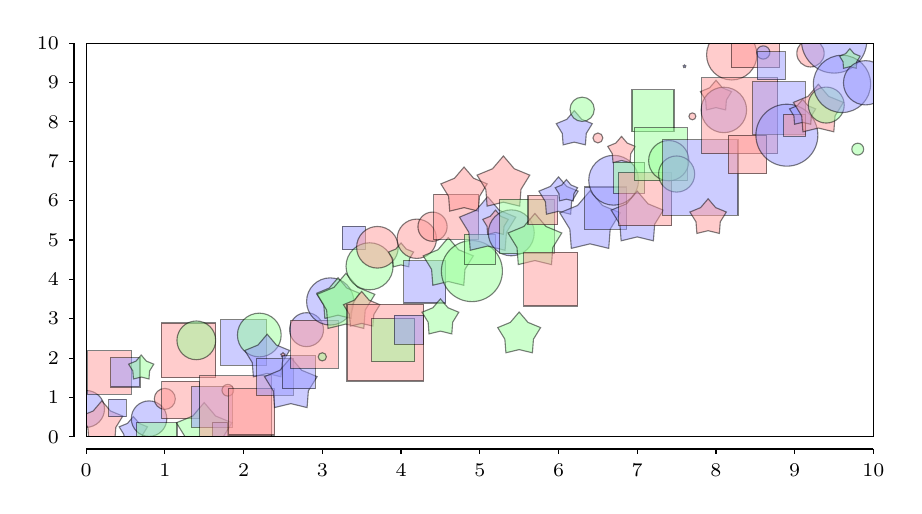
\begin{tikzpicture}
\begin{scope}[]
\pgfpathmoveto{ \pgfpointxy {0.0} {0.0}}
\pgfpathlineto{ \pgfpointxy {10.0} {0.0}}
\pgfpathlineto{ \pgfpointxy {10.0} {5.0}}
\pgfpathlineto{ \pgfpointxy {0.0} {5.0}}
\pgfpathclose
\pgfusepath{  clip, }
\begin{scope}[shift={(0.0,0.0)}]
\pgfsetxvec{\pgfpoint{1.0cm}{0cm}}
\pgfsetyvec{\pgfpoint{0cm}{0.5cm}}
\begin{scope}[shift={(0.0,0.0)}]
\node at (0.0,0.709579903064161) [draw=black,fill=blue!40,opacity=0.5,circle,inner sep=0.0mm,minimum width =4.684404387965109mm,minimum height=4.684404387965109mm] {};
\node at (0.1,-1.3086410799311836) [draw=black,fill=blue!40,opacity=0.5,circle,inner sep=0.0mm,minimum width =5.948432363904152mm,minimum height=5.948432363904152mm] {};
\node at (0.2,0.35464207368852163) [draw=black,fill=red!40,opacity=0.5,star,inner sep=0.0mm,minimum width =5.597520769773753mm,minimum height=5.597520769773753mm] {};
\node at (0.3,1.6355035193942828) [draw=black,fill=red!40,opacity=0.5,rectangle,inner sep=0.0mm,minimum width =5.5289513760349704mm,minimum height=5.5289513760349704mm] {};
\node at (0.4,0.7275541529298895) [draw=black,fill=blue!40,opacity=0.5,rectangle,inner sep=0.0mm,minimum width =2.2165720989965196mm,minimum height=2.2165720989965196mm] {};
\node at (0.5,1.6345911300381193) [draw=black,fill=blue!40,opacity=0.5,rectangle,inner sep=0.0mm,minimum width =3.69348293691323mm,minimum height=3.69348293691323mm] {};
\node at (0.6,0.1372935667470575) [draw=black,fill=blue!40,opacity=0.5,star,inner sep=0.0mm,minimum width =3.783654313145048mm,minimum height=3.783654313145048mm] {};
\node at (0.7,1.7421867243340636) [draw=black,fill=green!40,opacity=0.5,star,inner sep=0.0mm,minimum width =3.3580720084876603mm,minimum height=3.3580720084876603mm] {};
\node at (0.8,0.4620408089043557) [draw=black,fill=blue!40,opacity=0.5,circle,inner sep=0.0mm,minimum width =4.510210384891336mm,minimum height=4.510210384891336mm] {};
\node at (0.90000004,-0.15530240728422862) [draw=black,fill=green!40,opacity=0.5,rectangle,inner sep=0.0mm,minimum width =5.100643838385599mm,minimum height=5.100643838385599mm] {};
\node at (1.0,0.9641748075000852) [draw=black,fill=red!40,opacity=0.5,circle,inner sep=0.0mm,minimum width =2.673701415640892mm,minimum height=2.673701415640892mm] {};
\node at (1.1,-1.1603107800518702) [draw=black,fill=green!40,opacity=0.5,circle,inner sep=0.0mm,minimum width =4.774274002638963mm,minimum height=4.774274002638963mm] {};
\node at (1.2,0.9334271294075822) [draw=black,fill=red!40,opacity=0.5,rectangle,inner sep=0.0mm,minimum width =4.740705628150259mm,minimum height=4.740705628150259mm] {};
\node at (1.3000001,2.196453840862024) [draw=black,fill=red!40,opacity=0.5,rectangle,inner sep=0.0mm,minimum width =6.953264139897893mm,minimum height=6.953264139897893mm] {};
\node at (1.4,2.4509401059034674) [draw=black,fill=green!40,opacity=0.5,circle,inner sep=0.0mm,minimum width =4.918409651642974mm,minimum height=4.918409651642974mm] {};
\node at (1.5,0.1287607390986354) [draw=black,fill=green!40,opacity=0.5,star,inner sep=0.0mm,minimum width =7.414065824401571mm,minimum height=7.414065824401571mm] {};
\node at (1.6,0.7619799504504053) [draw=black,fill=blue!40,opacity=0.5,rectangle,inner sep=0.0mm,minimum width =5.155594127275793mm,minimum height=5.155594127275793mm] {};
\node at (1.7,0.18446059842809426) [draw=black,fill=blue!40,opacity=0.5,rectangle,inner sep=0.0mm,minimum width =1.8236676531537817mm,minimum height=1.8236676531537817mm] {};
\node at (1.8000001,1.1832418888351939) [draw=black,fill=red!40,opacity=0.5,circle,inner sep=0.0mm,minimum width =1.483075043186194mm,minimum height=1.483075043186194mm] {};
\node at (1.9,0.6438811288709911) [draw=black,fill=red!40,opacity=0.5,rectangle,inner sep=0.0mm,minimum width =9.121229801796648mm,minimum height=9.121229801796648mm] {};
\node at (2.0,2.399988531779001) [draw=black,fill=blue!40,opacity=0.5,rectangle,inner sep=0.0mm,minimum width =5.790814399699697mm,minimum height=5.790814399699697mm] {};
\node at (2.1000001,0.6336931157661692) [draw=black,fill=red!40,opacity=0.5,rectangle,inner sep=0.0mm,minimum width =5.883046419335988mm,minimum height=5.883046419335988mm] {};
\node at (2.2,2.5863110861604133) [draw=black,fill=green!40,opacity=0.5,circle,inner sep=0.0mm,minimum width =5.5551403318859105mm,minimum height=5.5551403318859105mm] {};
\node at (2.3,2.0088235911851084) [draw=black,fill=blue!40,opacity=0.5,star,inner sep=0.0mm,minimum width =5.978204784282441mm,minimum height=5.978204784282441mm] {};
\node at (2.4,1.5184735280897157) [draw=black,fill=blue!40,opacity=0.5,rectangle,inner sep=0.0mm,minimum width =4.6291829657364465mm,minimum height=4.6291829657364465mm] {};
\node at (2.5,2.081125610249627) [draw=black,fill=red!40,opacity=0.5,star,inner sep=0.0mm,minimum width =0.5808451501325136mm,minimum height=0.5808451501325136mm] {};
\node at (2.6000001,1.312119941776202) [draw=black,fill=blue!40,opacity=0.5,star,inner sep=0.0mm,minimum width =7.028290655475499mm,minimum height=7.028290655475499mm] {};
\node at (2.7,1.637236852472321) [draw=black,fill=blue!40,opacity=0.5,rectangle,inner sep=0.0mm,minimum width =4.1993268052830075mm,minimum height=4.1993268052830075mm] {};
\node at (2.8,2.722482173813692) [draw=black,fill=blue!40,opacity=0.5,circle,inner sep=0.0mm,minimum width =4.310358115557271mm,minimum height=4.310358115557271mm] {};
\node at (2.9,2.3523726337683586) [draw=black,fill=red!40,opacity=0.5,rectangle,inner sep=0.0mm,minimum width =6.057682425604773mm,minimum height=6.057682425604773mm] {};
\node at (3.0,2.0324011303461686) [draw=black,fill=green!40,opacity=0.5,circle,inner sep=0.0mm,minimum width =1.040741659203983mm,minimum height=1.040741659203983mm] {};
\node at (3.1000001,3.438578408970455) [draw=black,fill=blue!40,opacity=0.5,circle,inner sep=0.0mm,minimum width =5.995604978545116mm,minimum height=5.995604978545116mm] {};
\node at (3.2,3.4707427399239204) [draw=black,fill=green!40,opacity=0.5,star,inner sep=0.0mm,minimum width =5.710271475224298mm,minimum height=5.710271475224298mm] {};
\node at (3.3,3.379956079683047) [draw=black,fill=green!40,opacity=0.5,star,inner sep=0.0mm,minimum width =7.728879228930112mm,minimum height=7.728879228930112mm] {};
\node at (3.4,5.050936643838629) [draw=black,fill=blue!40,opacity=0.5,rectangle,inner sep=0.0mm,minimum width =2.9447285286666793mm,minimum height=2.9447285286666793mm] {};
\node at (3.5,3.2059979135589516) [draw=black,fill=red!40,opacity=0.5,star,inner sep=0.0mm,minimum width =4.868690569045189mm,minimum height=4.868690569045189mm] {};
\node at (3.6000001,4.3317506628087346) [draw=black,fill=green!40,opacity=0.5,circle,inner sep=0.0mm,minimum width =5.9754418095417074mm,minimum height=5.9754418095417074mm] {};
\node at (3.7,4.814904111132433) [draw=black,fill=red!40,opacity=0.5,circle,inner sep=0.0mm,minimum width =5.288882938019944mm,minimum height=5.288882938019944mm] {};
\node at (3.8,2.391690563293844) [draw=black,fill=red!40,opacity=0.5,rectangle,inner sep=0.0mm,minimum width =9.728440412869261mm,minimum height=9.728440412869261mm] {};
\node at (3.9,2.4498473067093514) [draw=black,fill=green!40,opacity=0.5,rectangle,inner sep=0.0mm,minimum width =5.4504184785211285mm,minimum height=5.4504184785211285mm] {};
\node at (4.0,4.589797853575581) [draw=black,fill=green!40,opacity=0.5,star,inner sep=0.0mm,minimum width =3.345428851666787mm,minimum height=3.345428851666787mm] {};
\node at (4.1,2.724158727310493) [draw=black,fill=blue!40,opacity=0.5,rectangle,inner sep=0.0mm,minimum width =3.6857011733674985mm,minimum height=3.6857011733674985mm] {};
\node at (4.2000003,5.0312764967330335) [draw=black,fill=red!40,opacity=0.5,circle,inner sep=0.0mm,minimum width =4.99519411089988mm,minimum height=4.99519411089988mm] {};
\node at (4.3,3.9348257471569066) [draw=black,fill=blue!40,opacity=0.5,rectangle,inner sep=0.0mm,minimum width =5.342270493568651mm,minimum height=5.342270493568651mm] {};
\node at (4.4,5.338033392113277) [draw=black,fill=red!40,opacity=0.5,circle,inner sep=0.0mm,minimum width =3.7076063582040835mm,minimum height=3.7076063582040835mm] {};
\node at (4.5,3.0129312560328323) [draw=black,fill=green!40,opacity=0.5,star,inner sep=0.0mm,minimum width =4.915535481344827mm,minimum height=4.915535481344827mm] {};
\node at (4.6,4.391119711430295) [draw=black,fill=green!40,opacity=0.5,star,inner sep=0.0mm,minimum width =6.688042568893176mm,minimum height=6.688042568893176mm] {};
\node at (4.7000003,5.591383230065377) [draw=black,fill=red!40,opacity=0.5,rectangle,inner sep=0.0mm,minimum width =5.7519680846567285mm,minimum height=5.7519680846567285mm] {};
\node at (4.8,6.234222310646458) [draw=black,fill=red!40,opacity=0.5,star,inner sep=0.0mm,minimum width =6.184886136008688mm,minimum height=6.184886136008688mm] {};
\node at (4.9,4.209886428794572) [draw=black,fill=green!40,opacity=0.5,circle,inner sep=0.0mm,minimum width =7.751415253945929mm,minimum height=7.751415253945929mm] {};
\node at (5.0,4.755880432357692) [draw=black,fill=green!40,opacity=0.5,rectangle,inner sep=0.0mm,minimum width =3.8890127528464298mm,minimum height=3.8890127528464298mm] {};
\node at (5.1,5.3477000912201715) [draw=black,fill=blue!40,opacity=0.5,star,inner sep=0.0mm,minimum width =7.526335426537427mm,minimum height=7.526335426537427mm] {};
\node at (5.2000003,5.417931536150252) [draw=black,fill=red!40,opacity=0.5,star,inner sep=0.0mm,minimum width =3.4041274521367972mm,minimum height=3.4041274521367972mm] {};
\node at (5.3,6.429576407662067) [draw=black,fill=red!40,opacity=0.5,star,inner sep=0.0mm,minimum width =7.039430589098215mm,minimum height=7.039430589098215mm] {};
\node at (5.4,5.181675135474579) [draw=black,fill=blue!40,opacity=0.5,circle,inner sep=0.0mm,minimum width =5.834549515289233mm,minimum height=5.834549515289233mm] {};
\node at (5.5,2.5976924743430176) [draw=black,fill=green!40,opacity=0.5,star,inner sep=0.0mm,minimum width =5.726956630012717mm,minimum height=5.726956630012717mm] {};
\node at (5.6,5.3464564714372385) [draw=black,fill=green!40,opacity=0.5,rectangle,inner sep=0.0mm,minimum width =6.918251071691451mm,minimum height=6.918251071691451mm] {};
\node at (5.7000003,4.955877499941573) [draw=black,fill=green!40,opacity=0.5,star,inner sep=0.0mm,minimum width =7.172585364535882mm,minimum height=7.172585364535882mm] {};
\node at (5.8,5.759435972163345) [draw=black,fill=red!40,opacity=0.5,rectangle,inner sep=0.0mm,minimum width =3.748330385692702mm,minimum height=3.748330385692702mm] {};
\node at (5.9,4.0057586223783614) [draw=black,fill=red!40,opacity=0.5,rectangle,inner sep=0.0mm,minimum width =6.833996499144574mm,minimum height=6.833996499144574mm] {};
\node at (6.0,6.078449060959694) [draw=black,fill=blue!40,opacity=0.5,star,inner sep=0.0mm,minimum width =5.241633459643229mm,minimum height=5.241633459643229mm] {};
\node at (6.1,6.235333726267953) [draw=black,fill=blue!40,opacity=0.5,star,inner sep=0.0mm,minimum width =2.985956986357431mm,minimum height=2.985956986357431mm] {};
\node at (6.2000003,7.805821875211378) [draw=black,fill=blue!40,opacity=0.5,star,inner sep=0.0mm,minimum width =4.809608886822457mm,minimum height=4.809608886822457mm] {};
\node at (6.3,8.319371400068796) [draw=black,fill=green!40,opacity=0.5,circle,inner sep=0.0mm,minimum width =3.085440678902571mm,minimum height=3.085440678902571mm] {};
\node at (6.4,5.440523454685933) [draw=black,fill=blue!40,opacity=0.5,star,inner sep=0.0mm,minimum width =8.079206783465558mm,minimum height=8.079206783465558mm] {};
\node at (6.5,7.591380850405745) [draw=black,fill=red!40,opacity=0.5,circle,inner sep=0.0mm,minimum width =1.26125656443805mm,minimum height=1.26125656443805mm] {};
\node at (6.6,5.809880770618726) [draw=black,fill=blue!40,opacity=0.5,rectangle,inner sep=0.0mm,minimum width =5.362748780650496mm,minimum height=5.362748780650496mm] {};
\node at (6.7000003,6.517662178130475) [draw=black,fill=blue!40,opacity=0.5,circle,inner sep=0.0mm,minimum width =6.330035823174752mm,minimum height=6.330035823174752mm] {};
\node at (6.8,7.263575252156768) [draw=black,fill=red!40,opacity=0.5,star,inner sep=0.0mm,minimum width =3.676561799349223mm,minimum height=3.676561799349223mm] {};
\node at (6.9,6.579734263794732) [draw=black,fill=green!40,opacity=0.5,rectangle,inner sep=0.0mm,minimum width =3.927892601102249mm,minimum height=3.927892601102249mm] {};
\node at (7.0,5.542746932789217) [draw=black,fill=blue!40,opacity=0.5,star,inner sep=0.0mm,minimum width =6.969794123179845mm,minimum height=6.969794123179845mm] {};
\node at (7.1,6.0379059430394335) [draw=black,fill=red!40,opacity=0.5,rectangle,inner sep=0.0mm,minimum width =6.7506325879376075mm,minimum height=6.7506325879376075mm] {};
\node at (7.2000003,8.280480967768897) [draw=black,fill=green!40,opacity=0.5,rectangle,inner sep=0.0mm,minimum width =5.339018829852397mm,minimum height=5.339018829852397mm] {};
\node at (7.3,7.182181103254856) [draw=black,fill=green!40,opacity=0.5,rectangle,inner sep=0.0mm,minimum width =6.725686399791425mm,minimum height=6.725686399791425mm] {};
\node at (7.4,7.015090870693126) [draw=black,fill=green!40,opacity=0.5,circle,inner sep=0.0mm,minimum width =5.116292902518763mm,minimum height=5.116292902518763mm] {};
\node at (7.5,6.6751307236389446) [draw=black,fill=green!40,opacity=0.5,circle,inner sep=0.0mm,minimum width =4.5886004252744215mm,minimum height=4.5886004252744215mm] {};
\node at (7.6,9.410407124352714) [draw=black,fill=blue!40,opacity=0.5,star,inner sep=0.0mm,minimum width =0.37060896034966095mm,minimum height=0.37060896034966095mm] {};
\node at (7.7000003,8.140927107356378) [draw=black,fill=red!40,opacity=0.5,circle,inner sep=0.0mm,minimum width =0.8827583798508689mm,minimum height=0.8827583798508689mm] {};
\node at (7.8,6.583624611015621) [draw=black,fill=blue!40,opacity=0.5,rectangle,inner sep=0.0mm,minimum width =9.578863669417665mm,minimum height=9.578863669417665mm] {};
\node at (7.9,5.560201118464219) [draw=black,fill=red!40,opacity=0.5,star,inner sep=0.0mm,minimum width =4.860793324924122mm,minimum height=4.860793324924122mm] {};
\node at (8.0,8.639981116539632) [draw=black,fill=red!40,opacity=0.5,star,inner sep=0.0mm,minimum width =4.162766116800425mm,minimum height=4.162766116800425mm] {};
\node at (8.1,8.303644538923303) [draw=black,fill=blue!40,opacity=0.5,circle,inner sep=0.0mm,minimum width =5.770867712632467mm,minimum height=5.770867712632467mm] {};
\node at (8.2,9.703646858790462) [draw=black,fill=red!40,opacity=0.5,circle,inner sep=0.0mm,minimum width =6.396720373224374mm,minimum height=6.396720373224374mm] {};
\node at (8.3,8.155916965941177) [draw=black,fill=red!40,opacity=0.5,rectangle,inner sep=0.0mm,minimum width =9.644834651219291mm,minimum height=9.644834651219291mm] {};
\node at (8.400001,7.174165890526005) [draw=black,fill=red!40,opacity=0.5,rectangle,inner sep=0.0mm,minimum width =4.906876252406299mm,minimum height=4.906876252406299mm] {};
\node at (8.5,9.993501200998535) [draw=black,fill=red!40,opacity=0.5,rectangle,inner sep=0.0mm,minimum width =6.129063146565033mm,minimum height=6.129063146565033mm] {};
\node at (8.6,9.762693058922483) [draw=black,fill=blue!40,opacity=0.5,circle,inner sep=0.0mm,minimum width =1.6863173325882124mm,minimum height=1.6863173325882124mm] {};
\node at (8.7,9.422479164772078) [draw=black,fill=blue!40,opacity=0.5,rectangle,inner sep=0.0mm,minimum width =3.539595339226378mm,minimum height=3.539595339226378mm] {};
\node at (8.8,8.354163852330503) [draw=black,fill=blue!40,opacity=0.5,rectangle,inner sep=0.0mm,minimum width =6.703053545363841mm,minimum height=6.703053545363841mm] {};
\node at (8.900001,7.661757948540961) [draw=black,fill=blue!40,opacity=0.5,circle,inner sep=0.0mm,minimum width =7.86719464912952mm,minimum height=7.86719464912952mm] {};
\node at (9.0,7.91234951291926) [draw=black,fill=red!40,opacity=0.5,rectangle,inner sep=0.0mm,minimum width =2.7938716367781504mm,minimum height=2.7938716367781504mm] {};
\node at (9.1,8.2216765832652) [draw=black,fill=blue!40,opacity=0.5,star,inner sep=0.0mm,minimum width =3.4920413472365164mm,minimum height=3.4920413472365164mm] {};
\node at (9.2,9.74173618895407) [draw=black,fill=red!40,opacity=0.5,circle,inner sep=0.0mm,minimum width =3.4747671534501894mm,minimum height=3.4747671534501894mm] {};
\node at (9.3,8.288177729457805) [draw=black,fill=red!40,opacity=0.5,star,inner sep=0.0mm,minimum width =6.675978200671102mm,minimum height=6.675978200671102mm] {};
\node at (9.400001,8.427125138594215) [draw=black,fill=green!40,opacity=0.5,circle,inner sep=0.0mm,minimum width =4.569844182184172mm,minimum height=4.569844182184172mm] {};
\node at (9.5,10.069225544328464) [draw=black,fill=blue!40,opacity=0.5,circle,inner sep=0.0mm,minimum width =8.30152077184257mm,minimum height=8.30152077184257mm] {};
\node at (9.6,8.964366331939702) [draw=black,fill=blue!40,opacity=0.5,circle,inner sep=0.0mm,minimum width =7.275475075209899mm,minimum height=7.275475075209899mm] {};
\node at (9.7,9.584259098836835) [draw=black,fill=green!40,opacity=0.5,star,inner sep=0.0mm,minimum width =2.745311571399896mm,minimum height=2.745311571399896mm] {};
\node at (9.8,7.307211115035337) [draw=black,fill=green!40,opacity=0.5,circle,inner sep=0.0mm,minimum width =1.510095726531878mm,minimum height=1.510095726531878mm] {};
\node at (9.900001,8.993141124791453) [draw=black,fill=blue!40,opacity=0.5,circle,inner sep=0.0mm,minimum width =5.6241368858900005mm,minimum height=5.6241368858900005mm] {};
\end{scope}
\pgfsetxvec{\pgfpoint{1cm}{0cm}}
\pgfsetyvec{\pgfpoint{0cm}{1cm}}
\end{scope}
\end{scope}
\begin{scope}[shift={(0.0,0.0)}]
\pgfsetxvec{\pgfpoint{1.0cm}{0cm}}
\pgfsetyvec{\pgfpoint{0cm}{0.5cm}}
\begin{scope}[shift={(0.0,0.0)}]
\begin{scope}[thin]
\pgfpathmoveto{ \pgfpointxy {0.0} {0.0}}
\pgfpathlineto{ \pgfpointxy {10.0} {0.0}}
\pgfpathlineto{ \pgfpointxy {10.0} {10.0}}
\pgfpathlineto{ \pgfpointxy {0.0} {10.0}}
\pgfpathclose
\pgfusepath{ stroke, }
\end{scope}
\begin{scope}[yshift=0cm]
\end{scope}
\begin{scope}[xshift=0cm]
\end{scope}
\begin{scope}[thick,black,fill=white]
\pgfpointadd{\pgfpointxy {0.0} {0.0}} {\pgfpoint{0}{-0.15cm}}\pgfpathmoveto{ NIL }
\pgfpointadd{\pgfpointxy {10.0} {0.0}} {\pgfpoint{0}{-0.15cm}}\pgfpathlineto{ NIL }
\pgfpointadd{\pgfpointxy {0.0} {0.0}} {\pgfpoint{-0.15cm}{0}}\pgfpathmoveto{ NIL }
\pgfpointadd{\pgfpointxy {0.0} {10.0}} {\pgfpoint{-0.15cm}{0}}\pgfpathlineto{ NIL }
\pgfusepath{ stroke, }
\end{scope}
\begin{scope}[yshift=-0.15cm]
\draw[] [shift={(0.0,0.0)}] (0,0) -- (0,-2pt) node[below]{ \scriptsize{\num[round-mode=places,round-precision=0]{0}}};
\draw[] [shift={(1.0,0.0)}] (0,0) -- (0,-2pt) node[below]{ \scriptsize{\num[round-mode=places,round-precision=0]{1}}};
\draw[] [shift={(2.0,0.0)}] (0,0) -- (0,-2pt) node[below]{ \scriptsize{\num[round-mode=places,round-precision=0]{2}}};
\draw[] [shift={(3.0,0.0)}] (0,0) -- (0,-2pt) node[below]{ \scriptsize{\num[round-mode=places,round-precision=0]{3}}};
\draw[] [shift={(4.0,0.0)}] (0,0) -- (0,-2pt) node[below]{ \scriptsize{\num[round-mode=places,round-precision=0]{4}}};
\draw[] [shift={(5.0,0.0)}] (0,0) -- (0,-2pt) node[below]{ \scriptsize{\num[round-mode=places,round-precision=0]{5}}};
\draw[] [shift={(6.0,0.0)}] (0,0) -- (0,-2pt) node[below]{ \scriptsize{\num[round-mode=places,round-precision=0]{6}}};
\draw[] [shift={(7.0,0.0)}] (0,0) -- (0,-2pt) node[below]{ \scriptsize{\num[round-mode=places,round-precision=0]{7}}};
\draw[] [shift={(8.0,0.0)}] (0,0) -- (0,-2pt) node[below]{ \scriptsize{\num[round-mode=places,round-precision=0]{8}}};
\draw[] [shift={(9.0,0.0)}] (0,0) -- (0,-2pt) node[below]{ \scriptsize{\num[round-mode=places,round-precision=0]{9}}};
\draw[] [shift={(10.0,0.0)}] (0,0) -- (0,-2pt) node[below]{ \scriptsize{\num[round-mode=places,round-precision=0]{10}}};
\end{scope}
\begin{scope}[xshift=-0.15cm]
\draw[] [shift={(0.0,0.0)}] (0,0) -- (-2pt,0) node[left]{ \scriptsize{\num[round-mode=places,round-precision=0]{0}}};
\draw[] [shift={(0.0,1.0)}] (0,0) -- (-2pt,0) node[left]{ \scriptsize{\num[round-mode=places,round-precision=0]{1}}};
\draw[] [shift={(0.0,2.0)}] (0,0) -- (-2pt,0) node[left]{ \scriptsize{\num[round-mode=places,round-precision=0]{2}}};
\draw[] [shift={(0.0,3.0)}] (0,0) -- (-2pt,0) node[left]{ \scriptsize{\num[round-mode=places,round-precision=0]{3}}};
\draw[] [shift={(0.0,4.0)}] (0,0) -- (-2pt,0) node[left]{ \scriptsize{\num[round-mode=places,round-precision=0]{4}}};
\draw[] [shift={(0.0,5.0)}] (0,0) -- (-2pt,0) node[left]{ \scriptsize{\num[round-mode=places,round-precision=0]{5}}};
\draw[] [shift={(0.0,6.0)}] (0,0) -- (-2pt,0) node[left]{ \scriptsize{\num[round-mode=places,round-precision=0]{6}}};
\draw[] [shift={(0.0,7.0)}] (0,0) -- (-2pt,0) node[left]{ \scriptsize{\num[round-mode=places,round-precision=0]{7}}};
\draw[] [shift={(0.0,8.0)}] (0,0) -- (-2pt,0) node[left]{ \scriptsize{\num[round-mode=places,round-precision=0]{8}}};
\draw[] [shift={(0.0,9.0)}] (0,0) -- (-2pt,0) node[left]{ \scriptsize{\num[round-mode=places,round-precision=0]{9}}};
\draw[] [shift={(0.0,10.0)}] (0,0) -- (-2pt,0) node[left]{ \scriptsize{\num[round-mode=places,round-precision=0]{10}}};
\end{scope}
\end{scope}
\pgfsetxvec{\pgfpoint{1cm}{0cm}}
\pgfsetyvec{\pgfpoint{0cm}{1cm}}
\end{scope}
\end{tikzpicture}
\end{document}

  \caption{Nodes of different sizes.}
\end{figure}

\begin{figure}[H]
  \centering
  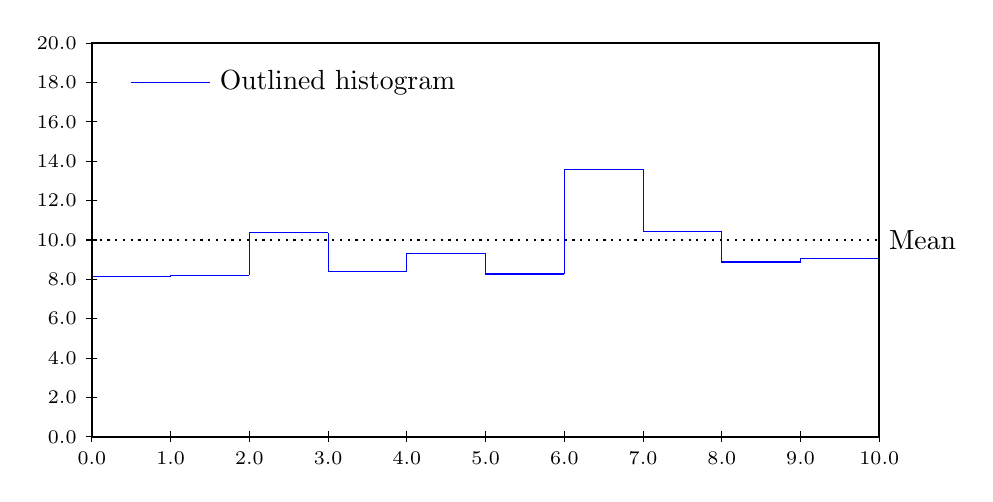
\begin{tikzpicture}
\begin{scope}[]
\clip (0,0) rectangle (10,5);
\begin{scope}[blue]
\draw[] (0.0,2.040753989729346) -- (1.0,2.040753989729346);
\draw (1.0,2.040753989729346) -- (1.0,2.0520371396851527) -- (2.0,2.0520371396851527);
\draw (2.0,2.0520371396851527) -- (2.0,2.589490136587087) -- (3.0,2.589490136587087);
\draw (3.0,2.589490136587087) -- (3.0,2.10531930397396) -- (4.0,2.10531930397396);
\draw (4.0,2.10531930397396) -- (4.0,2.328047479221825) -- (5.0,2.328047479221825);
\draw (5.0,2.328047479221825) -- (5.0,2.067390163042384) -- (6.0,2.067390163042384);
\draw (6.0,2.067390163042384) -- (6.0,3.3961419895360887) -- (7.0,3.3961419895360887);
\draw (7.0,3.3961419895360887) -- (7.0,2.6085288458106475) -- (8.0,2.6085288458106475);
\draw (8.0,2.6085288458106475) -- (8.0,2.2210174657245827) -- (9.0,2.2210174657245827);
\draw (9.0,2.2210174657245827) -- (9.0,2.2670683657782047) -- (10.0,2.2670683657782047);
\end{scope}
\end{scope}
\draw (0,0cm + 2pt) -- (0, 0cm -2pt) node[below] {\scriptsize{\num[round-mode=places,round-precision=1]{0}}};
\draw (1,0cm + 2pt) -- (1, 0cm -2pt) node[below] {\scriptsize{\num[round-mode=places,round-precision=1]{1}}};
\draw (2,0cm + 2pt) -- (2, 0cm -2pt) node[below] {\scriptsize{\num[round-mode=places,round-precision=1]{2}}};
\draw (3,0cm + 2pt) -- (3, 0cm -2pt) node[below] {\scriptsize{\num[round-mode=places,round-precision=1]{3}}};
\draw (4,0cm + 2pt) -- (4, 0cm -2pt) node[below] {\scriptsize{\num[round-mode=places,round-precision=1]{4}}};
\draw (5,0cm + 2pt) -- (5, 0cm -2pt) node[below] {\scriptsize{\num[round-mode=places,round-precision=1]{5}}};
\draw (6,0cm + 2pt) -- (6, 0cm -2pt) node[below] {\scriptsize{\num[round-mode=places,round-precision=1]{6}}};
\draw (7,0cm + 2pt) -- (7, 0cm -2pt) node[below] {\scriptsize{\num[round-mode=places,round-precision=1]{7}}};
\draw (8,0cm + 2pt) -- (8, 0cm -2pt) node[below] {\scriptsize{\num[round-mode=places,round-precision=1]{8}}};
\draw (9,0cm + 2pt) -- (9, 0cm -2pt) node[below] {\scriptsize{\num[round-mode=places,round-precision=1]{9}}};
\draw (10,0cm + 2pt) -- (10, 0cm -2pt) node[below] {\scriptsize{\num[round-mode=places,round-precision=1]{10}}};
\draw (0cm + 2pt,0.    ) -- (0cm-2pt,0.    ) node[left] {\scriptsize{\num[round-mode=places,round-precision=1]{0}}};
\draw (0cm + 2pt,0.5    ) -- (0cm-2pt,0.5    ) node[left] {\scriptsize{\num[round-mode=places,round-precision=1]{2}}};
\draw (0cm + 2pt,1.    ) -- (0cm-2pt,1.    ) node[left] {\scriptsize{\num[round-mode=places,round-precision=1]{4}}};
\draw (0cm + 2pt,1.5    ) -- (0cm-2pt,1.5    ) node[left] {\scriptsize{\num[round-mode=places,round-precision=1]{6}}};
\draw (0cm + 2pt,2.    ) -- (0cm-2pt,2.    ) node[left] {\scriptsize{\num[round-mode=places,round-precision=1]{8}}};
\draw (0cm + 2pt,2.5    ) -- (0cm-2pt,2.5    ) node[left] {\scriptsize{\num[round-mode=places,round-precision=1]{10}}};
\draw (0cm + 2pt,3.    ) -- (0cm-2pt,3.    ) node[left] {\scriptsize{\num[round-mode=places,round-precision=1]{12}}};
\draw (0cm + 2pt,3.5    ) -- (0cm-2pt,3.5    ) node[left] {\scriptsize{\num[round-mode=places,round-precision=1]{14}}};
\draw (0cm + 2pt,4.    ) -- (0cm-2pt,4.    ) node[left] {\scriptsize{\num[round-mode=places,round-precision=1]{16}}};
\draw (0cm + 2pt,4.5    ) -- (0cm-2pt,4.5    ) node[left] {\scriptsize{\num[round-mode=places,round-precision=1]{18}}};
\draw (0cm + 2pt,5.    ) -- (0cm-2pt,5.    ) node[left] {\scriptsize{\num[round-mode=places,round-precision=1]{20}}};
\draw[thick] (0,0) rectangle (10,5);
\draw[thick,dotted] (0.0,2.5) -- (10.0,2.5);
\node[right] at (10.0,2.5) {Mean};
\draw[blue] (0.5,4.5) -- (1.5,4.5);
\node[right,] at (1.5,4.5) {Outlined histogram};
\end{tikzpicture}
%%% Local Variables: 
%%% mode: latex 
%%% TeX-master: "master" 
%%% End:


  \caption{Another histogram}
\end{figure}

\begin{figure}[H]
  \centering
  %%% AUTO GENERATED CODE
\documentclass{standalone}
\ifx\HCode\UnDef\else\def\pgfsysdriver{pgfsys-tex4ht.def}\fi
\usepackage[usenames,dvipsnames,svgnames,table]{xcolor}
\usepackage{tikz}
\usepackage{color}
\usepackage{siunitx}
\usetikzlibrary{arrows,shapes}
\begin{document}
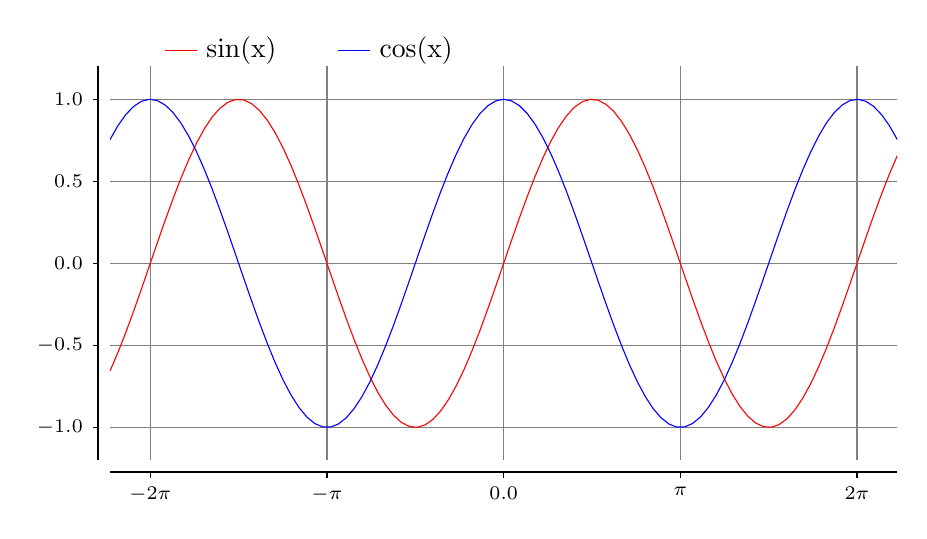
\begin{tikzpicture}
\begin{scope}[shift={(0.0,0.0)}]
\pgfsetxvec{\pgfpoint{0.71428573cm}{0cm}}
\pgfsetyvec{\pgfpoint{0cm}{2.0833333cm}}
\begin{scope}[shift={(7.0,1.2)}]
\begin{scope}[thin,gray]
\pgfpathmoveto{ \pgfpointxy {-6.283185307179586} {-1.2}}
\pgfpathlineto{ \pgfpointxy {-6.283185307179586} {1.2}}
\pgfpathmoveto{ \pgfpointxy {-3.141592653589793} {-1.2}}
\pgfpathlineto{ \pgfpointxy {-3.141592653589793} {1.2}}
\pgfpathmoveto{ \pgfpointxy {0.0} {-1.2}}
\pgfpathlineto{ \pgfpointxy {0.0} {1.2}}
\pgfpathmoveto{ \pgfpointxy {3.141592653589793} {-1.2}}
\pgfpathlineto{ \pgfpointxy {3.141592653589793} {1.2}}
\pgfpathmoveto{ \pgfpointxy {6.283185307179586} {-1.2}}
\pgfpathlineto{ \pgfpointxy {6.283185307179586} {1.2}}
\pgfpathmoveto{ \pgfpointxy {-7.0} {-1.0}}
\pgfpathlineto{ \pgfpointxy {7.0} {-1.0}}
\pgfpathmoveto{ \pgfpointxy {-7.0} {-0.5}}
\pgfpathlineto{ \pgfpointxy {7.0} {-0.5}}
\pgfpathmoveto{ \pgfpointxy {-7.0} {0.0}}
\pgfpathlineto{ \pgfpointxy {7.0} {0.0}}
\pgfpathmoveto{ \pgfpointxy {-7.0} {0.5}}
\pgfpathlineto{ \pgfpointxy {7.0} {0.5}}
\pgfpathmoveto{ \pgfpointxy {-7.0} {1.0}}
\pgfpathlineto{ \pgfpointxy {7.0} {1.0}}
\pgfusepath{ stroke, }
\end{scope}
\end{scope}
\pgfsetxvec{\pgfpoint{1cm}{0cm}}
\pgfsetyvec{\pgfpoint{0cm}{1cm}}
\end{scope}
\begin{scope}[shift={(0.0,0.0)}]
\pgfsetxvec{\pgfpoint{0.71428573cm}{0cm}}
\pgfsetyvec{\pgfpoint{0cm}{2.0833333cm}}
\begin{scope}[shift={(7.0,1.2)}]
\begin{scope}[thick,black,fill=white]
\pgfpathmoveto{ \pgfpointadd{\pgfpointxy {-7.0} {-1.2}} {\pgfpoint{0}{-0.15cm}} }
\pgfpathlineto{ \pgfpointadd{\pgfpointxy {7.0} {-1.2}} {\pgfpoint{0}{-0.15cm}} }
\pgfpathmoveto{ \pgfpointadd{\pgfpointxy {-7.0} {-1.2}} {\pgfpoint{-0.15cm}{0}} }
\pgfpathlineto{ \pgfpointadd{\pgfpointxy {-7.0} {1.2}} {\pgfpoint{-0.15cm}{0}} }
\pgfusepath{ stroke, }
\end{scope}
\begin{scope}[yshift=-0.15cm]
\draw[] [shift={(-6.283185307179586,-1.2)}] (0,0) -- (0,-2pt) node[below]{ \scriptsize{$-2\pi$}};
\draw[] [shift={(-3.141592653589793,-1.2)}] (0,0) -- (0,-2pt) node[below]{ \scriptsize{$-\pi$}};
\draw[] [shift={(0.0,-1.2)}] (0,0) -- (0,-2pt) node[below]{ \scriptsize{0.0}};
\draw[] [shift={(3.141592653589793,-1.2)}] (0,0) -- (0,-2pt) node[below]{ \scriptsize{$\pi$}};
\draw[] [shift={(6.283185307179586,-1.2)}] (0,0) -- (0,-2pt) node[below]{ \scriptsize{$2\pi$}};
\end{scope}
\begin{scope}[xshift=-0.15cm]
\draw[] [shift={(-7.0,-1.0)}] (0,0) -- (-2pt,0) node[left]{ \scriptsize{\num[round-mode=places,round-precision=1]{-1.0}}};
\draw[] [shift={(-7.0,-0.5)}] (0,0) -- (-2pt,0) node[left]{ \scriptsize{\num[round-mode=places,round-precision=1]{-0.5}}};
\draw[] [shift={(-7.0,0.0)}] (0,0) -- (-2pt,0) node[left]{ \scriptsize{\num[round-mode=places,round-precision=1]{0.0}}};
\draw[] [shift={(-7.0,0.5)}] (0,0) -- (-2pt,0) node[left]{ \scriptsize{\num[round-mode=places,round-precision=1]{0.5}}};
\draw[] [shift={(-7.0,1.0)}] (0,0) -- (-2pt,0) node[left]{ \scriptsize{\num[round-mode=places,round-precision=1]{1.0}}};
\end{scope}
\end{scope}
\pgfsetxvec{\pgfpoint{1cm}{0cm}}
\pgfsetyvec{\pgfpoint{0cm}{1cm}}
\end{scope}
\begin{scope}[]
\pgfpathmoveto{ \pgfpointadd{\pgfpointxy {0.0} {0.0}} {\pgfpoint{0cm}{0cm}} }
\pgfpathlineto{ \pgfpointadd{\pgfpointxy {0.0} {0.0}} {\pgfpoint{10cm}{0cm}} }
\pgfpathlineto{ \pgfpointadd{\pgfpointxy {0.0} {0.0}} {\pgfpoint{10cm}{5cm}} }
\pgfpathlineto{ \pgfpointadd{\pgfpointxy {0.0} {0.0}} {\pgfpoint{0cm}{5cm}} }
\pgfpathclose
\pgfusepath{  clip, }
\begin{scope}[shift={(0.0,0.0)}]
\pgfsetxvec{\pgfpoint{0.71428573cm}{0cm}}
\pgfsetyvec{\pgfpoint{0cm}{2.0833333cm}}
\begin{scope}[shift={(7.0,1.2)}]
\begin{scope}[red]
\pgfpathmoveto{ \pgfpointxy {-7.0} {-0.6569866}}
\pgfpathlineto{ \pgfpointxy {-6.86} {-0.54535675}}
\pgfpathlineto{ \pgfpointxy {-6.72} {-0.4230554}}
\pgfpathlineto{ \pgfpointxy {-6.58} {-0.29247567}}
\pgfpathlineto{ \pgfpointxy {-6.44} {-0.15617278}}
\pgfpathlineto{ \pgfpointxy {-6.3} {-0.0168139}}
\pgfpathlineto{ \pgfpointxy {-6.16} {0.12287399}}
\pgfpathlineto{ \pgfpointxy {-6.02} {0.2601575}}
\pgfpathlineto{ \pgfpointxy {-5.88} {0.39235023}}
\pgfpathlineto{ \pgfpointxy {-5.74} {0.51686543}}
\pgfpathlineto{ \pgfpointxy {-5.6} {0.63126665}}
\pgfpathlineto{ \pgfpointxy {-5.46} {0.7333152}}
\pgfpathlineto{ \pgfpointxy {-5.32} {0.8210142}}
\pgfpathlineto{ \pgfpointxy {-5.18} {0.8926477}}
\pgfpathlineto{ \pgfpointxy {-5.04} {0.94681376}}
\pgfpathlineto{ \pgfpointxy {-4.9} {0.98245263}}
\pgfpathlineto{ \pgfpointxy {-4.76} {0.9988668}}
\pgfpathlineto{ \pgfpointxy {-4.62} {0.99573517}}
\pgfpathlineto{ \pgfpointxy {-4.48} {0.97311896}}
\pgfpathlineto{ \pgfpointxy {-4.34} {0.9314608}}
\pgfpathlineto{ \pgfpointxy {-4.2} {0.8715758}}
\pgfpathlineto{ \pgfpointxy {-4.06} {0.7946358}}
\pgfpathlineto{ \pgfpointxy {-3.92} {0.7021463}}
\pgfpathlineto{ \pgfpointxy {-3.78} {0.5959172}}
\pgfpathlineto{ \pgfpointxy {-3.64} {0.47802725}}
\pgfpathlineto{ \pgfpointxy {-3.5} {0.35078323}}
\pgfpathlineto{ \pgfpointxy {-3.36} {0.21667509}}
\pgfpathlineto{ \pgfpointxy {-3.22} {0.07832703}}
\pgfpathlineto{ \pgfpointxy {-3.08} {-0.061553717}}
\pgfpathlineto{ \pgfpointxy {-2.94} {-0.20022999}}
\pgfpathlineto{ \pgfpointxy {-2.8} {-0.33498815}}
\pgfpathlineto{ \pgfpointxy {-2.66} {-0.46319127}}
\pgfpathlineto{ \pgfpointxy {-2.52} {-0.58233064}}
\pgfpathlineto{ \pgfpointxy {-2.38} {-0.690075}}
\pgfpathlineto{ \pgfpointxy {-2.24} {-0.78431594}}
\pgfpathlineto{ \pgfpointxy {-2.1} {-0.86320937}}
\pgfpathlineto{ \pgfpointxy {-1.96} {-0.92521155}}
\pgfpathlineto{ \pgfpointxy {-1.82} {-0.9691091}}
\pgfpathlineto{ \pgfpointxy {-1.68} {-0.99404323}}
\pgfpathlineto{ \pgfpointxy {-1.54} {-0.99952585}}
\pgfpathlineto{ \pgfpointxy {-1.4} {-0.98544973}}
\pgfpathlineto{ \pgfpointxy {-1.26} {-0.9520903}}
\pgfpathlineto{ \pgfpointxy {-1.12} {-0.90010047}}
\pgfpathlineto{ \pgfpointxy {-0.98} {-0.8304974}}
\pgfpathlineto{ \pgfpointxy {-0.84} {-0.7446431}}
\pgfpathlineto{ \pgfpointxy {-0.7} {-0.64421767}}
\pgfpathlineto{ \pgfpointxy {-0.56} {-0.5311862}}
\pgfpathlineto{ \pgfpointxy {-0.42} {-0.40776044}}
\pgfpathlineto{ \pgfpointxy {-0.28} {-0.27635565}}
\pgfpathlineto{ \pgfpointxy {-0.14} {-0.13954312}}
\pgfpathlineto{ \pgfpointxy {0.0} {0.0}}
\pgfpathlineto{ \pgfpointxy {0.14} {0.13954312}}
\pgfpathlineto{ \pgfpointxy {0.28} {0.27635565}}
\pgfpathlineto{ \pgfpointxy {0.42} {0.40776044}}
\pgfpathlineto{ \pgfpointxy {0.56} {0.5311862}}
\pgfpathlineto{ \pgfpointxy {0.7} {0.64421767}}
\pgfpathlineto{ \pgfpointxy {0.84} {0.7446431}}
\pgfpathlineto{ \pgfpointxy {0.98} {0.8304974}}
\pgfpathlineto{ \pgfpointxy {1.12} {0.90010047}}
\pgfpathlineto{ \pgfpointxy {1.26} {0.9520903}}
\pgfpathlineto{ \pgfpointxy {1.4} {0.98544973}}
\pgfpathlineto{ \pgfpointxy {1.54} {0.99952585}}
\pgfpathlineto{ \pgfpointxy {1.68} {0.99404323}}
\pgfpathlineto{ \pgfpointxy {1.82} {0.9691091}}
\pgfpathlineto{ \pgfpointxy {1.96} {0.92521155}}
\pgfpathlineto{ \pgfpointxy {2.1} {0.86320937}}
\pgfpathlineto{ \pgfpointxy {2.24} {0.78431594}}
\pgfpathlineto{ \pgfpointxy {2.38} {0.690075}}
\pgfpathlineto{ \pgfpointxy {2.52} {0.58233064}}
\pgfpathlineto{ \pgfpointxy {2.66} {0.46319127}}
\pgfpathlineto{ \pgfpointxy {2.8} {0.33498815}}
\pgfpathlineto{ \pgfpointxy {2.94} {0.20022999}}
\pgfpathlineto{ \pgfpointxy {3.08} {0.061553717}}
\pgfpathlineto{ \pgfpointxy {3.22} {-0.07832703}}
\pgfpathlineto{ \pgfpointxy {3.36} {-0.21667509}}
\pgfpathlineto{ \pgfpointxy {3.5} {-0.35078323}}
\pgfpathlineto{ \pgfpointxy {3.64} {-0.47802725}}
\pgfpathlineto{ \pgfpointxy {3.78} {-0.5959172}}
\pgfpathlineto{ \pgfpointxy {3.92} {-0.7021463}}
\pgfpathlineto{ \pgfpointxy {4.06} {-0.7946358}}
\pgfpathlineto{ \pgfpointxy {4.2} {-0.8715758}}
\pgfpathlineto{ \pgfpointxy {4.34} {-0.9314608}}
\pgfpathlineto{ \pgfpointxy {4.48} {-0.97311896}}
\pgfpathlineto{ \pgfpointxy {4.62} {-0.99573517}}
\pgfpathlineto{ \pgfpointxy {4.76} {-0.9988668}}
\pgfpathlineto{ \pgfpointxy {4.9} {-0.98245263}}
\pgfpathlineto{ \pgfpointxy {5.04} {-0.94681376}}
\pgfpathlineto{ \pgfpointxy {5.18} {-0.8926477}}
\pgfpathlineto{ \pgfpointxy {5.32} {-0.8210142}}
\pgfpathlineto{ \pgfpointxy {5.46} {-0.7333152}}
\pgfpathlineto{ \pgfpointxy {5.6} {-0.63126665}}
\pgfpathlineto{ \pgfpointxy {5.74} {-0.51686543}}
\pgfpathlineto{ \pgfpointxy {5.88} {-0.39235023}}
\pgfpathlineto{ \pgfpointxy {6.02} {-0.2601575}}
\pgfpathlineto{ \pgfpointxy {6.16} {-0.12287399}}
\pgfpathlineto{ \pgfpointxy {6.3} {0.0168139}}
\pgfpathlineto{ \pgfpointxy {6.44} {0.15617278}}
\pgfpathlineto{ \pgfpointxy {6.58} {0.29247567}}
\pgfpathlineto{ \pgfpointxy {6.72} {0.4230554}}
\pgfpathlineto{ \pgfpointxy {6.86} {0.54535675}}
\pgfpathlineto{ \pgfpointxy {7.0} {0.6569866}}
\pgfusepath{ stroke, }
\end{scope}
\end{scope}
\pgfsetxvec{\pgfpoint{1cm}{0cm}}
\pgfsetyvec{\pgfpoint{0cm}{1cm}}
\end{scope}
\end{scope}
\draw[red] (0.7,5.2) -- (1.1,5.2);
\node at (1.1,5.2) [right,,] {sin(x)};
\begin{scope}[]
\pgfpathmoveto{ \pgfpointadd{\pgfpointxy {0.0} {0.0}} {\pgfpoint{0cm}{0cm}} }
\pgfpathlineto{ \pgfpointadd{\pgfpointxy {0.0} {0.0}} {\pgfpoint{10cm}{0cm}} }
\pgfpathlineto{ \pgfpointadd{\pgfpointxy {0.0} {0.0}} {\pgfpoint{10cm}{5cm}} }
\pgfpathlineto{ \pgfpointadd{\pgfpointxy {0.0} {0.0}} {\pgfpoint{0cm}{5cm}} }
\pgfpathclose
\pgfusepath{  clip, }
\begin{scope}[shift={(0.0,0.0)}]
\pgfsetxvec{\pgfpoint{0.71428573cm}{0cm}}
\pgfsetyvec{\pgfpoint{0cm}{2.0833333cm}}
\begin{scope}[shift={(7.0,1.2)}]
\begin{scope}[blue]
\pgfpathmoveto{ \pgfpointxy {-7.0} {0.75390226}}
\pgfpathlineto{ \pgfpointxy {-6.86} {0.838204}}
\pgfpathlineto{ \pgfpointxy {-6.72} {0.9061038}}
\pgfpathlineto{ \pgfpointxy {-6.58} {0.95627296}}
\pgfpathlineto{ \pgfpointxy {-6.44} {0.9877297}}
\pgfpathlineto{ \pgfpointxy {-6.3} {0.9998586}}
\pgfpathlineto{ \pgfpointxy {-6.16} {0.9924223}}
\pgfpathlineto{ \pgfpointxy {-6.02} {0.9655662}}
\pgfpathlineto{ \pgfpointxy {-5.88} {0.9198159}}
\pgfpathlineto{ \pgfpointxy {-5.74} {0.85606664}}
\pgfpathlineto{ \pgfpointxy {-5.6} {0.77556586}}
\pgfpathlineto{ \pgfpointxy {-5.46} {0.67988884}}
\pgfpathlineto{ \pgfpointxy {-5.32} {0.5709077}}
\pgfpathlineto{ \pgfpointxy {-5.18} {0.45075506}}
\pgfpathlineto{ \pgfpointxy {-5.04} {0.32178202}}
\pgfpathlineto{ \pgfpointxy {-4.9} {0.18651237}}
\pgfpathlineto{ \pgfpointxy {-4.76} {0.047593035}}
\pgfpathlineto{ \pgfpointxy {-4.62} {-0.092257604}}
\pgfpathlineto{ \pgfpointxy {-4.48} {-0.23030294}}
\pgfpathlineto{ \pgfpointxy {-4.34} {-0.3638417}}
\pgfpathlineto{ \pgfpointxy {-4.2} {-0.4902608}}
\pgfpathlineto{ \pgfpointxy {-4.06} {-0.6070865}}
\pgfpathlineto{ \pgfpointxy {-3.92} {-0.71203274}}
\pgfpathlineto{ \pgfpointxy {-3.78} {-0.80304587}}
\pgfpathlineto{ \pgfpointxy {-3.64} {-0.878345}}
\pgfpathlineto{ \pgfpointxy {-3.5} {-0.9364567}}
\pgfpathlineto{ \pgfpointxy {-3.36} {-0.9762438}}
\pgfpathlineto{ \pgfpointxy {-3.22} {-0.99692774}}
\pgfpathlineto{ \pgfpointxy {-3.08} {-0.9981038}}
\pgfpathlineto{ \pgfpointxy {-2.94} {-0.9797489}}
\pgfpathlineto{ \pgfpointxy {-2.8} {-0.94222236}}
\pgfpathlineto{ \pgfpointxy {-2.66} {-0.88625836}}
\pgfpathlineto{ \pgfpointxy {-2.52} {-0.81295204}}
\pgfpathlineto{ \pgfpointxy {-2.38} {-0.7237379}}
\pgfpathlineto{ \pgfpointxy {-2.24} {-0.6203616}}
\pgfpathlineto{ \pgfpointxy {-2.1} {-0.5048461}}
\pgfpathlineto{ \pgfpointxy {-1.96} {-0.37945175}}
\pgfpathlineto{ \pgfpointxy {-1.82} {-0.24663231}}
\pgfpathlineto{ \pgfpointxy {-1.68} {-0.10898675}}
\pgfpathlineto{ \pgfpointxy {-1.54} {0.03079146}}
\pgfpathlineto{ \pgfpointxy {-1.4} {0.16996714}}
\pgfpathlineto{ \pgfpointxy {-1.26} {0.30581692}}
\pgfpathlineto{ \pgfpointxy {-1.12} {0.43568245}}
\pgfpathlineto{ \pgfpointxy {-0.98} {0.5570226}}
\pgfpathlineto{ \pgfpointxy {-0.84} {0.6674628}}
\pgfpathlineto{ \pgfpointxy {-0.7} {0.7648422}}
\pgfpathlineto{ \pgfpointxy {-0.56} {0.8472551}}
\pgfpathlineto{ \pgfpointxy {-0.42} {0.9130889}}
\pgfpathlineto{ \pgfpointxy {-0.28} {0.96105546}}
\pgfpathlineto{ \pgfpointxy {-0.14} {0.990216}}
\pgfpathlineto{ \pgfpointxy {0.0} {1.0}}
\pgfpathlineto{ \pgfpointxy {0.14} {0.990216}}
\pgfpathlineto{ \pgfpointxy {0.28} {0.96105546}}
\pgfpathlineto{ \pgfpointxy {0.42} {0.9130889}}
\pgfpathlineto{ \pgfpointxy {0.56} {0.8472551}}
\pgfpathlineto{ \pgfpointxy {0.7} {0.7648422}}
\pgfpathlineto{ \pgfpointxy {0.84} {0.6674628}}
\pgfpathlineto{ \pgfpointxy {0.98} {0.5570226}}
\pgfpathlineto{ \pgfpointxy {1.12} {0.43568245}}
\pgfpathlineto{ \pgfpointxy {1.26} {0.30581692}}
\pgfpathlineto{ \pgfpointxy {1.4} {0.16996714}}
\pgfpathlineto{ \pgfpointxy {1.54} {0.03079146}}
\pgfpathlineto{ \pgfpointxy {1.68} {-0.10898675}}
\pgfpathlineto{ \pgfpointxy {1.82} {-0.24663231}}
\pgfpathlineto{ \pgfpointxy {1.96} {-0.37945175}}
\pgfpathlineto{ \pgfpointxy {2.1} {-0.5048461}}
\pgfpathlineto{ \pgfpointxy {2.24} {-0.6203616}}
\pgfpathlineto{ \pgfpointxy {2.38} {-0.7237379}}
\pgfpathlineto{ \pgfpointxy {2.52} {-0.81295204}}
\pgfpathlineto{ \pgfpointxy {2.66} {-0.88625836}}
\pgfpathlineto{ \pgfpointxy {2.8} {-0.94222236}}
\pgfpathlineto{ \pgfpointxy {2.94} {-0.9797489}}
\pgfpathlineto{ \pgfpointxy {3.08} {-0.9981038}}
\pgfpathlineto{ \pgfpointxy {3.22} {-0.99692774}}
\pgfpathlineto{ \pgfpointxy {3.36} {-0.9762438}}
\pgfpathlineto{ \pgfpointxy {3.5} {-0.9364567}}
\pgfpathlineto{ \pgfpointxy {3.64} {-0.878345}}
\pgfpathlineto{ \pgfpointxy {3.78} {-0.80304587}}
\pgfpathlineto{ \pgfpointxy {3.92} {-0.71203274}}
\pgfpathlineto{ \pgfpointxy {4.06} {-0.6070865}}
\pgfpathlineto{ \pgfpointxy {4.2} {-0.4902608}}
\pgfpathlineto{ \pgfpointxy {4.34} {-0.3638417}}
\pgfpathlineto{ \pgfpointxy {4.48} {-0.23030294}}
\pgfpathlineto{ \pgfpointxy {4.62} {-0.092257604}}
\pgfpathlineto{ \pgfpointxy {4.76} {0.047593035}}
\pgfpathlineto{ \pgfpointxy {4.9} {0.18651237}}
\pgfpathlineto{ \pgfpointxy {5.04} {0.32178202}}
\pgfpathlineto{ \pgfpointxy {5.18} {0.45075506}}
\pgfpathlineto{ \pgfpointxy {5.32} {0.5709077}}
\pgfpathlineto{ \pgfpointxy {5.46} {0.67988884}}
\pgfpathlineto{ \pgfpointxy {5.6} {0.77556586}}
\pgfpathlineto{ \pgfpointxy {5.74} {0.85606664}}
\pgfpathlineto{ \pgfpointxy {5.88} {0.9198159}}
\pgfpathlineto{ \pgfpointxy {6.02} {0.9655662}}
\pgfpathlineto{ \pgfpointxy {6.16} {0.9924223}}
\pgfpathlineto{ \pgfpointxy {6.3} {0.9998586}}
\pgfpathlineto{ \pgfpointxy {6.44} {0.9877297}}
\pgfpathlineto{ \pgfpointxy {6.58} {0.95627296}}
\pgfpathlineto{ \pgfpointxy {6.72} {0.9061038}}
\pgfpathlineto{ \pgfpointxy {6.86} {0.838204}}
\pgfpathlineto{ \pgfpointxy {7.0} {0.75390226}}
\pgfusepath{ stroke, }
\end{scope}
\end{scope}
\pgfsetxvec{\pgfpoint{1cm}{0cm}}
\pgfsetyvec{\pgfpoint{0cm}{1cm}}
\end{scope}
\end{scope}
\draw[blue] (2.9,5.2) -- (3.3000002,5.2);
\node at (3.3000002,5.2) [right,,] {cos(x)};
\end{tikzpicture}
\end{document}

  \caption{Plotting functions}
\end{figure}

\begin{figure}[H]
  \centering
  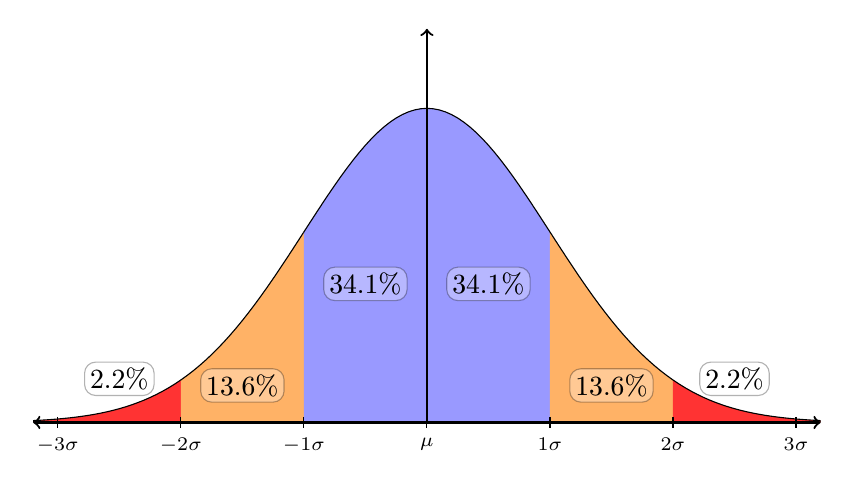
\begin{tikzpicture}[]
\begin{scope}[]
\clip (0,0) rectangle (10,5);
\begin{scope}[shift={(5.0,-0.0)}]
\pgfsetxvec{\pgfpoint{1.5625cm}{0cm}}
\pgfsetyvec{\pgfpoint{0cm}{10.0cm}}
\begin{scope}[]
\clip (-3.5,0) rectangle (-2,5);
\begin{scope}[fill=red!80]
\pgfpathmoveto{ \pgfqpointxy {-3.2} {0.0}}
\pgfpathlineto{ \pgfqpointxy {-3.2} {0.0023840873753184963}}
\pgfpathlineto{ \pgfqpointxy {-3.15} {0.002794257593560257}}
\pgfpathlineto{ \pgfqpointxy {-3.1000001} {0.0032668180294884892}}
\pgfpathlineto{ \pgfqpointxy {-3.05} {0.0038097626369961333}}
\pgfpathlineto{ \pgfqpointxy {-3.0} {0.004431848335480958}}
\pgfpathlineto{ \pgfqpointxy {-2.95} {0.005142640152435692}}
\pgfpathlineto{ \pgfqpointxy {-2.9} {0.0059525301721895674}}
\pgfpathlineto{ \pgfqpointxy {-2.8500001} {0.006872765030160735}}
\pgfpathlineto{ \pgfqpointxy {-2.8} {0.007915452600647405}}
\pgfpathlineto{ \pgfqpointxy {-2.75} {0.009093562739915748}}
\pgfpathlineto{ \pgfqpointxy {-2.7} {0.010420932487815211}}
\pgfpathlineto{ \pgfqpointxy {-2.65} {0.011912240802789813}}
\pgfpathlineto{ \pgfqpointxy {-2.6} {0.013582973636746678}}
\pgfpathlineto{ \pgfqpointxy {-2.55} {0.0154493503693536}}
\pgfpathlineto{ \pgfqpointxy {-2.5} {0.017528300772314036}}
\pgfpathlineto{ \pgfqpointxy {-2.45} {0.01983735428926949}}
\pgfpathlineto{ \pgfqpointxy {-2.4} {0.022394527829526112}}
\pgfpathlineto{ \pgfqpointxy {-2.35} {0.02521822470809983}}
\pgfpathlineto{ \pgfqpointxy {-2.3} {0.028327036984334027}}
\pgfpathlineto{ \pgfqpointxy {-2.25} {0.03173965331899954}}
\pgfpathlineto{ \pgfqpointxy {-2.2} {0.03547459146264942}}
\pgfpathlineto{ \pgfqpointxy {-2.15} {0.03955003329010437}}
\pgfpathlineto{ \pgfqpointxy {-2.1} {0.043983610791136565}}
\pgfpathlineto{ \pgfqpointxy {-2.0500002} {0.0487919988582986}}
\pgfpathlineto{ \pgfqpointxy {-2.0} {0.05399096581690089}}
\pgfpathlineto{ \pgfqpointxy {-1.95} {0.059594698701195395}}
\pgfpathlineto{ \pgfqpointxy {-1.9} {0.0656158210884853}}
\pgfpathlineto{ \pgfqpointxy {-1.85} {0.07206486699288937}}
\pgfpathlineto{ \pgfqpointxy {-1.8000001} {0.07895014710951938}}
\pgfpathlineto{ \pgfqpointxy {-1.75} {0.08627732079584774}}
\pgfpathlineto{ \pgfqpointxy {-1.7} {0.09404907505773316}}
\pgfpathlineto{ \pgfqpointxy {-1.65} {0.10226493431891748}}
\pgfpathlineto{ \pgfqpointxy {-1.6} {0.11092082645768998}}
\pgfpathlineto{ \pgfqpointxy {-1.5500001} {0.12000899363633905}}
\pgfpathlineto{ \pgfqpointxy {-1.5} {0.12951759400603588}}
\pgfpathlineto{ \pgfqpointxy {-1.45} {0.13943055308925387}}
\pgfpathlineto{ \pgfqpointxy {-1.4} {0.1497274686645169}}
\pgfpathlineto{ \pgfqpointxy {-1.35} {0.16038331353123803}}
\pgfpathlineto{ \pgfqpointxy {-1.3000001} {0.1713685781825969}}
\pgfpathlineto{ \pgfqpointxy {-1.25} {0.18264908057503657}}
\pgfpathlineto{ \pgfqpointxy {-1.2} {0.19418604935410852}}
\pgfpathlineto{ \pgfqpointxy {-1.1500001} {0.20593624274853736}}
\pgfpathlineto{ \pgfqpointxy {-1.0999999} {0.2178522101371628}}
\pgfpathlineto{ \pgfqpointxy {-1.05} {0.22988214937606208}}
\pgfpathlineto{ \pgfqpointxy {-1.0} {0.24197072716759546}}
\pgfpathlineto{ \pgfqpointxy {-0.95000005} {0.2540590433921869}}
\pgfpathlineto{ \pgfqpointxy {-0.9000001} {0.2660852255786465}}
\pgfpathlineto{ \pgfqpointxy {-0.8499999} {0.2779849044804291}}
\pgfpathlineto{ \pgfqpointxy {-0.79999995} {0.28969157075782764}}
\pgfpathlineto{ \pgfqpointxy {-0.75} {0.301137431015238}}
\pgfpathlineto{ \pgfqpointxy {-0.70000005} {0.3122539309350428}}
\pgfpathlineto{ \pgfqpointxy {-0.6500001} {0.3229723497479345}}
\pgfpathlineto{ \pgfqpointxy {-0.5999999} {0.33322460871255405}}
\pgfpathlineto{ \pgfqpointxy {-0.54999995} {0.3429438655858136}}
\pgfpathlineto{ \pgfqpointxy {-0.5} {0.3520653231025355}}
\pgfpathlineto{ \pgfqpointxy {-0.45000005} {0.3605269661186527}}
\pgfpathlineto{ \pgfqpointxy {-0.4000001} {0.368270132302718}}
\pgfpathlineto{ \pgfqpointxy {-0.3499999} {0.3752403681731694}}
\pgfpathlineto{ \pgfqpointxy {-0.29999995} {0.38138780955933627}}
\pgfpathlineto{ \pgfqpointxy {-0.25} {0.3866681089751429}}
\pgfpathlineto{ \pgfqpointxy {-0.20000005} {0.39104269718605056}}
\pgfpathlineto{ \pgfqpointxy {-0.1500001} {0.3944793301217544}}
\pgfpathlineto{ \pgfqpointxy {-0.099999905} {0.3969525406736286}}
\pgfpathlineto{ \pgfqpointxy {-0.049999952} {0.39844392404048146}}
\pgfpathlineto{ \pgfqpointxy {0.0} {0.3989422804014327}}
\pgfpathlineto{ \pgfqpointxy {0.049999952} {0.39844392404048146}}
\pgfpathlineto{ \pgfqpointxy {0.099999905} {0.3969525406736286}}
\pgfpathlineto{ \pgfqpointxy {0.1500001} {0.3944793301217544}}
\pgfpathlineto{ \pgfqpointxy {0.20000005} {0.39104269718605056}}
\pgfpathlineto{ \pgfqpointxy {0.25} {0.3866681089751429}}
\pgfpathlineto{ \pgfqpointxy {0.29999995} {0.38138780955933627}}
\pgfpathlineto{ \pgfqpointxy {0.3499999} {0.3752403681731694}}
\pgfpathlineto{ \pgfqpointxy {0.4000001} {0.368270132302718}}
\pgfpathlineto{ \pgfqpointxy {0.45000005} {0.3605269661186527}}
\pgfpathlineto{ \pgfqpointxy {0.5} {0.3520653231025355}}
\pgfpathlineto{ \pgfqpointxy {0.54999995} {0.3429438655858136}}
\pgfpathlineto{ \pgfqpointxy {0.5999999} {0.33322460871255405}}
\pgfpathlineto{ \pgfqpointxy {0.6500001} {0.3229723497479345}}
\pgfpathlineto{ \pgfqpointxy {0.70000005} {0.3122539309350428}}
\pgfpathlineto{ \pgfqpointxy {0.75} {0.301137431015238}}
\pgfpathlineto{ \pgfqpointxy {0.79999995} {0.28969157075782764}}
\pgfpathlineto{ \pgfqpointxy {0.85000014} {0.2779848569228033}}
\pgfpathlineto{ \pgfqpointxy {0.89999986} {0.2660852731362723}}
\pgfpathlineto{ \pgfqpointxy {0.95000005} {0.2540590433921869}}
\pgfpathlineto{ \pgfqpointxy {1.0000002} {0.24197065583115673}}
\pgfpathlineto{ \pgfqpointxy {1.05} {0.22988214937606208}}
\pgfpathlineto{ \pgfqpointxy {1.1000001} {0.21785213880072407}}
\pgfpathlineto{ \pgfqpointxy {1.1499999} {0.2059363140849761}}
\pgfpathlineto{ \pgfqpointxy {1.2} {0.19418604935410852}}
\pgfpathlineto{ \pgfqpointxy {1.2500002} {0.18264903301741073}}
\pgfpathlineto{ \pgfqpointxy {1.3} {0.1713686019614098}}
\pgfpathlineto{ \pgfqpointxy {1.3500001} {0.16038330164183157}}
\pgfpathlineto{ \pgfqpointxy {1.3999999} {0.14972750433273627}}
\pgfpathlineto{ \pgfqpointxy {1.45} {0.13943055308925387}}
\pgfpathlineto{ \pgfqpointxy {1.5000002} {0.12951754644841007}}
\pgfpathlineto{ \pgfqpointxy {1.55} {0.1200090055257455}}
\pgfpathlineto{ \pgfqpointxy {1.6000001} {0.11092081456828352}}
\pgfpathlineto{ \pgfqpointxy {1.6499999} {0.10226494620832394}}
\pgfpathlineto{ \pgfqpointxy {1.7} {0.09404907505773316}}
\pgfpathlineto{ \pgfqpointxy {1.7500002} {0.08627727918292515}}
\pgfpathlineto{ \pgfqpointxy {1.8} {0.07895016494362907}}
\pgfpathlineto{ \pgfqpointxy {1.8500001} {0.07206485510348291}}
\pgfpathlineto{ \pgfqpointxy {1.8999999} {0.06561583297789175}}
\pgfpathlineto{ \pgfqpointxy {1.95} {0.059594698701195395}}
\pgfpathlineto{ \pgfqpointxy {2.0000002} {0.053990942038087984}}
\pgfpathlineto{ \pgfqpointxy {2.05} {0.048792022637111514}}
\pgfpathlineto{ \pgfqpointxy {2.1000001} {0.043983578095268816}}
\pgfpathlineto{ \pgfqpointxy {2.1499999} {0.03955005112421405}}
\pgfpathlineto{ \pgfqpointxy {2.2} {0.03547459146264942}}
\pgfpathlineto{ \pgfqpointxy {2.2500002} {0.03173963548488986}}
\pgfpathlineto{ \pgfqpointxy {2.3} {0.028327036984334027}}
\pgfpathlineto{ \pgfqpointxy {2.3500001} {0.025218212818693374}}
\pgfpathlineto{ \pgfqpointxy {2.3999999} {0.02239453823275676}}
\pgfpathlineto{ \pgfqpointxy {2.45} {0.01983735428926949}}
\pgfpathlineto{ \pgfqpointxy {2.5000002} {0.017528287396731772}}
\pgfpathlineto{ \pgfqpointxy {2.55} {0.0154493503693536}}
\pgfpathlineto{ \pgfqpointxy {2.6000001} {0.013582964719691839}}
\pgfpathlineto{ \pgfqpointxy {2.6499999} {0.01191224897675675}}
\pgfpathlineto{ \pgfqpointxy {2.7} {0.010420932487815211}}
\pgfpathlineto{ \pgfqpointxy {2.7500002} {0.009093556052124616}}
\pgfpathlineto{ \pgfqpointxy {2.8} {0.007915452600647405}}
\pgfpathlineto{ \pgfqpointxy {2.8500001} {0.006872765030160735}}
\pgfpathlineto{ \pgfqpointxy {2.8999999} {0.005952535745348843}}
\pgfpathlineto{ \pgfqpointxy {2.95} {0.005142640152435692}}
\pgfpathlineto{ \pgfqpointxy {3.0000002} {0.004431844248497489}}
\pgfpathlineto{ \pgfqpointxy {3.05} {0.0038097626369961333}}
\pgfpathlineto{ \pgfqpointxy {3.1000001} {0.0032668180294884892}}
\pgfpathlineto{ \pgfqpointxy {3.1499999} {0.0027942601943679187}}
\pgfpathlineto{ \pgfqpointxy {3.2} {0.0023840873753184963}}
\pgfpathlineto{ \pgfqpointxy {3.2} {0.0}}
\pgfusepath{ fill,stroke }
\end{scope}
\end{scope}
\node at (-2.5,0.05546041322884499) [rectangle,inner sep=2pt,minimum width =2pt,minimum height=2pt,fill=white,opacity=0.3,draw=black, rounded corners] {2.2\%}; 
\node at (-2.5,0.05546041322884499) [rectangle,inner sep=0pt,minimum width =2pt,minimum height=2pt,text=black] {2.2\%}; 
\pgfsetxvec{\pgfpoint{1cm}{0cm}}
\pgfsetyvec{\pgfpoint{0cm}{1cm}}
\end{scope}
\end{scope}
\begin{scope}[]
\clip (0,0) rectangle (10,5);
\begin{scope}[shift={(5.0,-0.0)}]
\pgfsetxvec{\pgfpoint{1.5625cm}{0cm}}
\pgfsetyvec{\pgfpoint{0cm}{10.0cm}}
\begin{scope}[]
\clip (-2,0) rectangle (-1,5);
\begin{scope}[fill=orange!60]
\pgfpathmoveto{ \pgfqpointxy {-3.2} {0.0}}
\pgfpathlineto{ \pgfqpointxy {-3.2} {0.0023840873753184963}}
\pgfpathlineto{ \pgfqpointxy {-3.15} {0.002794257593560257}}
\pgfpathlineto{ \pgfqpointxy {-3.1000001} {0.0032668180294884892}}
\pgfpathlineto{ \pgfqpointxy {-3.05} {0.0038097626369961333}}
\pgfpathlineto{ \pgfqpointxy {-3.0} {0.004431848335480958}}
\pgfpathlineto{ \pgfqpointxy {-2.95} {0.005142640152435692}}
\pgfpathlineto{ \pgfqpointxy {-2.9} {0.0059525301721895674}}
\pgfpathlineto{ \pgfqpointxy {-2.8500001} {0.006872765030160735}}
\pgfpathlineto{ \pgfqpointxy {-2.8} {0.007915452600647405}}
\pgfpathlineto{ \pgfqpointxy {-2.75} {0.009093562739915748}}
\pgfpathlineto{ \pgfqpointxy {-2.7} {0.010420932487815211}}
\pgfpathlineto{ \pgfqpointxy {-2.65} {0.011912240802789813}}
\pgfpathlineto{ \pgfqpointxy {-2.6} {0.013582973636746678}}
\pgfpathlineto{ \pgfqpointxy {-2.55} {0.0154493503693536}}
\pgfpathlineto{ \pgfqpointxy {-2.5} {0.017528300772314036}}
\pgfpathlineto{ \pgfqpointxy {-2.45} {0.01983735428926949}}
\pgfpathlineto{ \pgfqpointxy {-2.4} {0.022394527829526112}}
\pgfpathlineto{ \pgfqpointxy {-2.35} {0.02521822470809983}}
\pgfpathlineto{ \pgfqpointxy {-2.3} {0.028327036984334027}}
\pgfpathlineto{ \pgfqpointxy {-2.25} {0.03173965331899954}}
\pgfpathlineto{ \pgfqpointxy {-2.2} {0.03547459146264942}}
\pgfpathlineto{ \pgfqpointxy {-2.15} {0.03955003329010437}}
\pgfpathlineto{ \pgfqpointxy {-2.1} {0.043983610791136565}}
\pgfpathlineto{ \pgfqpointxy {-2.0500002} {0.0487919988582986}}
\pgfpathlineto{ \pgfqpointxy {-2.0} {0.05399096581690089}}
\pgfpathlineto{ \pgfqpointxy {-1.95} {0.059594698701195395}}
\pgfpathlineto{ \pgfqpointxy {-1.9} {0.0656158210884853}}
\pgfpathlineto{ \pgfqpointxy {-1.85} {0.07206486699288937}}
\pgfpathlineto{ \pgfqpointxy {-1.8000001} {0.07895014710951938}}
\pgfpathlineto{ \pgfqpointxy {-1.75} {0.08627732079584774}}
\pgfpathlineto{ \pgfqpointxy {-1.7} {0.09404907505773316}}
\pgfpathlineto{ \pgfqpointxy {-1.65} {0.10226493431891748}}
\pgfpathlineto{ \pgfqpointxy {-1.6} {0.11092082645768998}}
\pgfpathlineto{ \pgfqpointxy {-1.5500001} {0.12000899363633905}}
\pgfpathlineto{ \pgfqpointxy {-1.5} {0.12951759400603588}}
\pgfpathlineto{ \pgfqpointxy {-1.45} {0.13943055308925387}}
\pgfpathlineto{ \pgfqpointxy {-1.4} {0.1497274686645169}}
\pgfpathlineto{ \pgfqpointxy {-1.35} {0.16038331353123803}}
\pgfpathlineto{ \pgfqpointxy {-1.3000001} {0.1713685781825969}}
\pgfpathlineto{ \pgfqpointxy {-1.25} {0.18264908057503657}}
\pgfpathlineto{ \pgfqpointxy {-1.2} {0.19418604935410852}}
\pgfpathlineto{ \pgfqpointxy {-1.1500001} {0.20593624274853736}}
\pgfpathlineto{ \pgfqpointxy {-1.0999999} {0.2178522101371628}}
\pgfpathlineto{ \pgfqpointxy {-1.05} {0.22988214937606208}}
\pgfpathlineto{ \pgfqpointxy {-1.0} {0.24197072716759546}}
\pgfpathlineto{ \pgfqpointxy {-0.95000005} {0.2540590433921869}}
\pgfpathlineto{ \pgfqpointxy {-0.9000001} {0.2660852255786465}}
\pgfpathlineto{ \pgfqpointxy {-0.8499999} {0.2779849044804291}}
\pgfpathlineto{ \pgfqpointxy {-0.79999995} {0.28969157075782764}}
\pgfpathlineto{ \pgfqpointxy {-0.75} {0.301137431015238}}
\pgfpathlineto{ \pgfqpointxy {-0.70000005} {0.3122539309350428}}
\pgfpathlineto{ \pgfqpointxy {-0.6500001} {0.3229723497479345}}
\pgfpathlineto{ \pgfqpointxy {-0.5999999} {0.33322460871255405}}
\pgfpathlineto{ \pgfqpointxy {-0.54999995} {0.3429438655858136}}
\pgfpathlineto{ \pgfqpointxy {-0.5} {0.3520653231025355}}
\pgfpathlineto{ \pgfqpointxy {-0.45000005} {0.3605269661186527}}
\pgfpathlineto{ \pgfqpointxy {-0.4000001} {0.368270132302718}}
\pgfpathlineto{ \pgfqpointxy {-0.3499999} {0.3752403681731694}}
\pgfpathlineto{ \pgfqpointxy {-0.29999995} {0.38138780955933627}}
\pgfpathlineto{ \pgfqpointxy {-0.25} {0.3866681089751429}}
\pgfpathlineto{ \pgfqpointxy {-0.20000005} {0.39104269718605056}}
\pgfpathlineto{ \pgfqpointxy {-0.1500001} {0.3944793301217544}}
\pgfpathlineto{ \pgfqpointxy {-0.099999905} {0.3969525406736286}}
\pgfpathlineto{ \pgfqpointxy {-0.049999952} {0.39844392404048146}}
\pgfpathlineto{ \pgfqpointxy {0.0} {0.3989422804014327}}
\pgfpathlineto{ \pgfqpointxy {0.049999952} {0.39844392404048146}}
\pgfpathlineto{ \pgfqpointxy {0.099999905} {0.3969525406736286}}
\pgfpathlineto{ \pgfqpointxy {0.1500001} {0.3944793301217544}}
\pgfpathlineto{ \pgfqpointxy {0.20000005} {0.39104269718605056}}
\pgfpathlineto{ \pgfqpointxy {0.25} {0.3866681089751429}}
\pgfpathlineto{ \pgfqpointxy {0.29999995} {0.38138780955933627}}
\pgfpathlineto{ \pgfqpointxy {0.3499999} {0.3752403681731694}}
\pgfpathlineto{ \pgfqpointxy {0.4000001} {0.368270132302718}}
\pgfpathlineto{ \pgfqpointxy {0.45000005} {0.3605269661186527}}
\pgfpathlineto{ \pgfqpointxy {0.5} {0.3520653231025355}}
\pgfpathlineto{ \pgfqpointxy {0.54999995} {0.3429438655858136}}
\pgfpathlineto{ \pgfqpointxy {0.5999999} {0.33322460871255405}}
\pgfpathlineto{ \pgfqpointxy {0.6500001} {0.3229723497479345}}
\pgfpathlineto{ \pgfqpointxy {0.70000005} {0.3122539309350428}}
\pgfpathlineto{ \pgfqpointxy {0.75} {0.301137431015238}}
\pgfpathlineto{ \pgfqpointxy {0.79999995} {0.28969157075782764}}
\pgfpathlineto{ \pgfqpointxy {0.85000014} {0.2779848569228033}}
\pgfpathlineto{ \pgfqpointxy {0.89999986} {0.2660852731362723}}
\pgfpathlineto{ \pgfqpointxy {0.95000005} {0.2540590433921869}}
\pgfpathlineto{ \pgfqpointxy {1.0000002} {0.24197065583115673}}
\pgfpathlineto{ \pgfqpointxy {1.05} {0.22988214937606208}}
\pgfpathlineto{ \pgfqpointxy {1.1000001} {0.21785213880072407}}
\pgfpathlineto{ \pgfqpointxy {1.1499999} {0.2059363140849761}}
\pgfpathlineto{ \pgfqpointxy {1.2} {0.19418604935410852}}
\pgfpathlineto{ \pgfqpointxy {1.2500002} {0.18264903301741073}}
\pgfpathlineto{ \pgfqpointxy {1.3} {0.1713686019614098}}
\pgfpathlineto{ \pgfqpointxy {1.3500001} {0.16038330164183157}}
\pgfpathlineto{ \pgfqpointxy {1.3999999} {0.14972750433273627}}
\pgfpathlineto{ \pgfqpointxy {1.45} {0.13943055308925387}}
\pgfpathlineto{ \pgfqpointxy {1.5000002} {0.12951754644841007}}
\pgfpathlineto{ \pgfqpointxy {1.55} {0.1200090055257455}}
\pgfpathlineto{ \pgfqpointxy {1.6000001} {0.11092081456828352}}
\pgfpathlineto{ \pgfqpointxy {1.6499999} {0.10226494620832394}}
\pgfpathlineto{ \pgfqpointxy {1.7} {0.09404907505773316}}
\pgfpathlineto{ \pgfqpointxy {1.7500002} {0.08627727918292515}}
\pgfpathlineto{ \pgfqpointxy {1.8} {0.07895016494362907}}
\pgfpathlineto{ \pgfqpointxy {1.8500001} {0.07206485510348291}}
\pgfpathlineto{ \pgfqpointxy {1.8999999} {0.06561583297789175}}
\pgfpathlineto{ \pgfqpointxy {1.95} {0.059594698701195395}}
\pgfpathlineto{ \pgfqpointxy {2.0000002} {0.053990942038087984}}
\pgfpathlineto{ \pgfqpointxy {2.05} {0.048792022637111514}}
\pgfpathlineto{ \pgfqpointxy {2.1000001} {0.043983578095268816}}
\pgfpathlineto{ \pgfqpointxy {2.1499999} {0.03955005112421405}}
\pgfpathlineto{ \pgfqpointxy {2.2} {0.03547459146264942}}
\pgfpathlineto{ \pgfqpointxy {2.2500002} {0.03173963548488986}}
\pgfpathlineto{ \pgfqpointxy {2.3} {0.028327036984334027}}
\pgfpathlineto{ \pgfqpointxy {2.3500001} {0.025218212818693374}}
\pgfpathlineto{ \pgfqpointxy {2.3999999} {0.02239453823275676}}
\pgfpathlineto{ \pgfqpointxy {2.45} {0.01983735428926949}}
\pgfpathlineto{ \pgfqpointxy {2.5000002} {0.017528287396731772}}
\pgfpathlineto{ \pgfqpointxy {2.55} {0.0154493503693536}}
\pgfpathlineto{ \pgfqpointxy {2.6000001} {0.013582964719691839}}
\pgfpathlineto{ \pgfqpointxy {2.6499999} {0.01191224897675675}}
\pgfpathlineto{ \pgfqpointxy {2.7} {0.010420932487815211}}
\pgfpathlineto{ \pgfqpointxy {2.7500002} {0.009093556052124616}}
\pgfpathlineto{ \pgfqpointxy {2.8} {0.007915452600647405}}
\pgfpathlineto{ \pgfqpointxy {2.8500001} {0.006872765030160735}}
\pgfpathlineto{ \pgfqpointxy {2.8999999} {0.005952535745348843}}
\pgfpathlineto{ \pgfqpointxy {2.95} {0.005142640152435692}}
\pgfpathlineto{ \pgfqpointxy {3.0000002} {0.004431844248497489}}
\pgfpathlineto{ \pgfqpointxy {3.05} {0.0038097626369961333}}
\pgfpathlineto{ \pgfqpointxy {3.1000001} {0.0032668180294884892}}
\pgfpathlineto{ \pgfqpointxy {3.1499999} {0.0027942601943679187}}
\pgfpathlineto{ \pgfqpointxy {3.2} {0.0023840873753184963}}
\pgfpathlineto{ \pgfqpointxy {3.2} {0.0}}
\pgfusepath{ fill,stroke }
\end{scope}
\end{scope}
\node at (-1.5,0.04702453752886658) [rectangle,inner sep=2pt,minimum width =2pt,minimum height=2pt,fill=white,opacity=0.3,draw=black, rounded corners] {13.6\%}; 
\node at (-1.5,0.04702453752886658) [rectangle,inner sep=0pt,minimum width =2pt,minimum height=2pt,text=black] {13.6\%}; 
\pgfsetxvec{\pgfpoint{1cm}{0cm}}
\pgfsetyvec{\pgfpoint{0cm}{1cm}}
\end{scope}
\end{scope}
\begin{scope}[]
\clip (0,0) rectangle (10,5);
\begin{scope}[shift={(5.0,-0.0)}]
\pgfsetxvec{\pgfpoint{1.5625cm}{0cm}}
\pgfsetyvec{\pgfpoint{0cm}{10.0cm}}
\begin{scope}[]
\clip (-1,0) rectangle (0,5);
\begin{scope}[fill=blue!40]
\pgfpathmoveto{ \pgfqpointxy {-3.2} {0.0}}
\pgfpathlineto{ \pgfqpointxy {-3.2} {0.0023840873753184963}}
\pgfpathlineto{ \pgfqpointxy {-3.15} {0.002794257593560257}}
\pgfpathlineto{ \pgfqpointxy {-3.1000001} {0.0032668180294884892}}
\pgfpathlineto{ \pgfqpointxy {-3.05} {0.0038097626369961333}}
\pgfpathlineto{ \pgfqpointxy {-3.0} {0.004431848335480958}}
\pgfpathlineto{ \pgfqpointxy {-2.95} {0.005142640152435692}}
\pgfpathlineto{ \pgfqpointxy {-2.9} {0.0059525301721895674}}
\pgfpathlineto{ \pgfqpointxy {-2.8500001} {0.006872765030160735}}
\pgfpathlineto{ \pgfqpointxy {-2.8} {0.007915452600647405}}
\pgfpathlineto{ \pgfqpointxy {-2.75} {0.009093562739915748}}
\pgfpathlineto{ \pgfqpointxy {-2.7} {0.010420932487815211}}
\pgfpathlineto{ \pgfqpointxy {-2.65} {0.011912240802789813}}
\pgfpathlineto{ \pgfqpointxy {-2.6} {0.013582973636746678}}
\pgfpathlineto{ \pgfqpointxy {-2.55} {0.0154493503693536}}
\pgfpathlineto{ \pgfqpointxy {-2.5} {0.017528300772314036}}
\pgfpathlineto{ \pgfqpointxy {-2.45} {0.01983735428926949}}
\pgfpathlineto{ \pgfqpointxy {-2.4} {0.022394527829526112}}
\pgfpathlineto{ \pgfqpointxy {-2.35} {0.02521822470809983}}
\pgfpathlineto{ \pgfqpointxy {-2.3} {0.028327036984334027}}
\pgfpathlineto{ \pgfqpointxy {-2.25} {0.03173965331899954}}
\pgfpathlineto{ \pgfqpointxy {-2.2} {0.03547459146264942}}
\pgfpathlineto{ \pgfqpointxy {-2.15} {0.03955003329010437}}
\pgfpathlineto{ \pgfqpointxy {-2.1} {0.043983610791136565}}
\pgfpathlineto{ \pgfqpointxy {-2.0500002} {0.0487919988582986}}
\pgfpathlineto{ \pgfqpointxy {-2.0} {0.05399096581690089}}
\pgfpathlineto{ \pgfqpointxy {-1.95} {0.059594698701195395}}
\pgfpathlineto{ \pgfqpointxy {-1.9} {0.0656158210884853}}
\pgfpathlineto{ \pgfqpointxy {-1.85} {0.07206486699288937}}
\pgfpathlineto{ \pgfqpointxy {-1.8000001} {0.07895014710951938}}
\pgfpathlineto{ \pgfqpointxy {-1.75} {0.08627732079584774}}
\pgfpathlineto{ \pgfqpointxy {-1.7} {0.09404907505773316}}
\pgfpathlineto{ \pgfqpointxy {-1.65} {0.10226493431891748}}
\pgfpathlineto{ \pgfqpointxy {-1.6} {0.11092082645768998}}
\pgfpathlineto{ \pgfqpointxy {-1.5500001} {0.12000899363633905}}
\pgfpathlineto{ \pgfqpointxy {-1.5} {0.12951759400603588}}
\pgfpathlineto{ \pgfqpointxy {-1.45} {0.13943055308925387}}
\pgfpathlineto{ \pgfqpointxy {-1.4} {0.1497274686645169}}
\pgfpathlineto{ \pgfqpointxy {-1.35} {0.16038331353123803}}
\pgfpathlineto{ \pgfqpointxy {-1.3000001} {0.1713685781825969}}
\pgfpathlineto{ \pgfqpointxy {-1.25} {0.18264908057503657}}
\pgfpathlineto{ \pgfqpointxy {-1.2} {0.19418604935410852}}
\pgfpathlineto{ \pgfqpointxy {-1.1500001} {0.20593624274853736}}
\pgfpathlineto{ \pgfqpointxy {-1.0999999} {0.2178522101371628}}
\pgfpathlineto{ \pgfqpointxy {-1.05} {0.22988214937606208}}
\pgfpathlineto{ \pgfqpointxy {-1.0} {0.24197072716759546}}
\pgfpathlineto{ \pgfqpointxy {-0.95000005} {0.2540590433921869}}
\pgfpathlineto{ \pgfqpointxy {-0.9000001} {0.2660852255786465}}
\pgfpathlineto{ \pgfqpointxy {-0.8499999} {0.2779849044804291}}
\pgfpathlineto{ \pgfqpointxy {-0.79999995} {0.28969157075782764}}
\pgfpathlineto{ \pgfqpointxy {-0.75} {0.301137431015238}}
\pgfpathlineto{ \pgfqpointxy {-0.70000005} {0.3122539309350428}}
\pgfpathlineto{ \pgfqpointxy {-0.6500001} {0.3229723497479345}}
\pgfpathlineto{ \pgfqpointxy {-0.5999999} {0.33322460871255405}}
\pgfpathlineto{ \pgfqpointxy {-0.54999995} {0.3429438655858136}}
\pgfpathlineto{ \pgfqpointxy {-0.5} {0.3520653231025355}}
\pgfpathlineto{ \pgfqpointxy {-0.45000005} {0.3605269661186527}}
\pgfpathlineto{ \pgfqpointxy {-0.4000001} {0.368270132302718}}
\pgfpathlineto{ \pgfqpointxy {-0.3499999} {0.3752403681731694}}
\pgfpathlineto{ \pgfqpointxy {-0.29999995} {0.38138780955933627}}
\pgfpathlineto{ \pgfqpointxy {-0.25} {0.3866681089751429}}
\pgfpathlineto{ \pgfqpointxy {-0.20000005} {0.39104269718605056}}
\pgfpathlineto{ \pgfqpointxy {-0.1500001} {0.3944793301217544}}
\pgfpathlineto{ \pgfqpointxy {-0.099999905} {0.3969525406736286}}
\pgfpathlineto{ \pgfqpointxy {-0.049999952} {0.39844392404048146}}
\pgfpathlineto{ \pgfqpointxy {0.0} {0.3989422804014327}}
\pgfpathlineto{ \pgfqpointxy {0.049999952} {0.39844392404048146}}
\pgfpathlineto{ \pgfqpointxy {0.099999905} {0.3969525406736286}}
\pgfpathlineto{ \pgfqpointxy {0.1500001} {0.3944793301217544}}
\pgfpathlineto{ \pgfqpointxy {0.20000005} {0.39104269718605056}}
\pgfpathlineto{ \pgfqpointxy {0.25} {0.3866681089751429}}
\pgfpathlineto{ \pgfqpointxy {0.29999995} {0.38138780955933627}}
\pgfpathlineto{ \pgfqpointxy {0.3499999} {0.3752403681731694}}
\pgfpathlineto{ \pgfqpointxy {0.4000001} {0.368270132302718}}
\pgfpathlineto{ \pgfqpointxy {0.45000005} {0.3605269661186527}}
\pgfpathlineto{ \pgfqpointxy {0.5} {0.3520653231025355}}
\pgfpathlineto{ \pgfqpointxy {0.54999995} {0.3429438655858136}}
\pgfpathlineto{ \pgfqpointxy {0.5999999} {0.33322460871255405}}
\pgfpathlineto{ \pgfqpointxy {0.6500001} {0.3229723497479345}}
\pgfpathlineto{ \pgfqpointxy {0.70000005} {0.3122539309350428}}
\pgfpathlineto{ \pgfqpointxy {0.75} {0.301137431015238}}
\pgfpathlineto{ \pgfqpointxy {0.79999995} {0.28969157075782764}}
\pgfpathlineto{ \pgfqpointxy {0.85000014} {0.2779848569228033}}
\pgfpathlineto{ \pgfqpointxy {0.89999986} {0.2660852731362723}}
\pgfpathlineto{ \pgfqpointxy {0.95000005} {0.2540590433921869}}
\pgfpathlineto{ \pgfqpointxy {1.0000002} {0.24197065583115673}}
\pgfpathlineto{ \pgfqpointxy {1.05} {0.22988214937606208}}
\pgfpathlineto{ \pgfqpointxy {1.1000001} {0.21785213880072407}}
\pgfpathlineto{ \pgfqpointxy {1.1499999} {0.2059363140849761}}
\pgfpathlineto{ \pgfqpointxy {1.2} {0.19418604935410852}}
\pgfpathlineto{ \pgfqpointxy {1.2500002} {0.18264903301741073}}
\pgfpathlineto{ \pgfqpointxy {1.3} {0.1713686019614098}}
\pgfpathlineto{ \pgfqpointxy {1.3500001} {0.16038330164183157}}
\pgfpathlineto{ \pgfqpointxy {1.3999999} {0.14972750433273627}}
\pgfpathlineto{ \pgfqpointxy {1.45} {0.13943055308925387}}
\pgfpathlineto{ \pgfqpointxy {1.5000002} {0.12951754644841007}}
\pgfpathlineto{ \pgfqpointxy {1.55} {0.1200090055257455}}
\pgfpathlineto{ \pgfqpointxy {1.6000001} {0.11092081456828352}}
\pgfpathlineto{ \pgfqpointxy {1.6499999} {0.10226494620832394}}
\pgfpathlineto{ \pgfqpointxy {1.7} {0.09404907505773316}}
\pgfpathlineto{ \pgfqpointxy {1.7500002} {0.08627727918292515}}
\pgfpathlineto{ \pgfqpointxy {1.8} {0.07895016494362907}}
\pgfpathlineto{ \pgfqpointxy {1.8500001} {0.07206485510348291}}
\pgfpathlineto{ \pgfqpointxy {1.8999999} {0.06561583297789175}}
\pgfpathlineto{ \pgfqpointxy {1.95} {0.059594698701195395}}
\pgfpathlineto{ \pgfqpointxy {2.0000002} {0.053990942038087984}}
\pgfpathlineto{ \pgfqpointxy {2.05} {0.048792022637111514}}
\pgfpathlineto{ \pgfqpointxy {2.1000001} {0.043983578095268816}}
\pgfpathlineto{ \pgfqpointxy {2.1499999} {0.03955005112421405}}
\pgfpathlineto{ \pgfqpointxy {2.2} {0.03547459146264942}}
\pgfpathlineto{ \pgfqpointxy {2.2500002} {0.03173963548488986}}
\pgfpathlineto{ \pgfqpointxy {2.3} {0.028327036984334027}}
\pgfpathlineto{ \pgfqpointxy {2.3500001} {0.025218212818693374}}
\pgfpathlineto{ \pgfqpointxy {2.3999999} {0.02239453823275676}}
\pgfpathlineto{ \pgfqpointxy {2.45} {0.01983735428926949}}
\pgfpathlineto{ \pgfqpointxy {2.5000002} {0.017528287396731772}}
\pgfpathlineto{ \pgfqpointxy {2.55} {0.0154493503693536}}
\pgfpathlineto{ \pgfqpointxy {2.6000001} {0.013582964719691839}}
\pgfpathlineto{ \pgfqpointxy {2.6499999} {0.01191224897675675}}
\pgfpathlineto{ \pgfqpointxy {2.7} {0.010420932487815211}}
\pgfpathlineto{ \pgfqpointxy {2.7500002} {0.009093556052124616}}
\pgfpathlineto{ \pgfqpointxy {2.8} {0.007915452600647405}}
\pgfpathlineto{ \pgfqpointxy {2.8500001} {0.006872765030160735}}
\pgfpathlineto{ \pgfqpointxy {2.8999999} {0.005952535745348843}}
\pgfpathlineto{ \pgfqpointxy {2.95} {0.005142640152435692}}
\pgfpathlineto{ \pgfqpointxy {3.0000002} {0.004431844248497489}}
\pgfpathlineto{ \pgfqpointxy {3.05} {0.0038097626369961333}}
\pgfpathlineto{ \pgfqpointxy {3.1000001} {0.0032668180294884892}}
\pgfpathlineto{ \pgfqpointxy {3.1499999} {0.0027942601943679187}}
\pgfpathlineto{ \pgfqpointxy {3.2} {0.0023840873753184963}}
\pgfpathlineto{ \pgfqpointxy {3.2} {0.0}}
\pgfusepath{ fill,stroke }
\end{scope}
\end{scope}
\node at (-0.5,0.17603266155126776) [rectangle,inner sep=2pt,minimum width =2pt,minimum height=2pt,fill=white,opacity=0.3,draw=black, rounded corners] {34.1\%}; 
\node at (-0.5,0.17603266155126776) [rectangle,inner sep=0pt,minimum width =2pt,minimum height=2pt,text=black] {34.1\%}; 
\pgfsetxvec{\pgfpoint{1cm}{0cm}}
\pgfsetyvec{\pgfpoint{0cm}{1cm}}
\end{scope}
\end{scope}
\begin{scope}[]
\clip (0,0) rectangle (10,5);
\begin{scope}[shift={(5.0,-0.0)}]
\pgfsetxvec{\pgfpoint{1.5625cm}{0cm}}
\pgfsetyvec{\pgfpoint{0cm}{10.0cm}}
\begin{scope}[]
\clip (0,0) rectangle (1,5);
\begin{scope}[fill=blue!40]
\pgfpathmoveto{ \pgfqpointxy {-3.2} {0.0}}
\pgfpathlineto{ \pgfqpointxy {-3.2} {0.0023840873753184963}}
\pgfpathlineto{ \pgfqpointxy {-3.15} {0.002794257593560257}}
\pgfpathlineto{ \pgfqpointxy {-3.1000001} {0.0032668180294884892}}
\pgfpathlineto{ \pgfqpointxy {-3.05} {0.0038097626369961333}}
\pgfpathlineto{ \pgfqpointxy {-3.0} {0.004431848335480958}}
\pgfpathlineto{ \pgfqpointxy {-2.95} {0.005142640152435692}}
\pgfpathlineto{ \pgfqpointxy {-2.9} {0.0059525301721895674}}
\pgfpathlineto{ \pgfqpointxy {-2.8500001} {0.006872765030160735}}
\pgfpathlineto{ \pgfqpointxy {-2.8} {0.007915452600647405}}
\pgfpathlineto{ \pgfqpointxy {-2.75} {0.009093562739915748}}
\pgfpathlineto{ \pgfqpointxy {-2.7} {0.010420932487815211}}
\pgfpathlineto{ \pgfqpointxy {-2.65} {0.011912240802789813}}
\pgfpathlineto{ \pgfqpointxy {-2.6} {0.013582973636746678}}
\pgfpathlineto{ \pgfqpointxy {-2.55} {0.0154493503693536}}
\pgfpathlineto{ \pgfqpointxy {-2.5} {0.017528300772314036}}
\pgfpathlineto{ \pgfqpointxy {-2.45} {0.01983735428926949}}
\pgfpathlineto{ \pgfqpointxy {-2.4} {0.022394527829526112}}
\pgfpathlineto{ \pgfqpointxy {-2.35} {0.02521822470809983}}
\pgfpathlineto{ \pgfqpointxy {-2.3} {0.028327036984334027}}
\pgfpathlineto{ \pgfqpointxy {-2.25} {0.03173965331899954}}
\pgfpathlineto{ \pgfqpointxy {-2.2} {0.03547459146264942}}
\pgfpathlineto{ \pgfqpointxy {-2.15} {0.03955003329010437}}
\pgfpathlineto{ \pgfqpointxy {-2.1} {0.043983610791136565}}
\pgfpathlineto{ \pgfqpointxy {-2.0500002} {0.0487919988582986}}
\pgfpathlineto{ \pgfqpointxy {-2.0} {0.05399096581690089}}
\pgfpathlineto{ \pgfqpointxy {-1.95} {0.059594698701195395}}
\pgfpathlineto{ \pgfqpointxy {-1.9} {0.0656158210884853}}
\pgfpathlineto{ \pgfqpointxy {-1.85} {0.07206486699288937}}
\pgfpathlineto{ \pgfqpointxy {-1.8000001} {0.07895014710951938}}
\pgfpathlineto{ \pgfqpointxy {-1.75} {0.08627732079584774}}
\pgfpathlineto{ \pgfqpointxy {-1.7} {0.09404907505773316}}
\pgfpathlineto{ \pgfqpointxy {-1.65} {0.10226493431891748}}
\pgfpathlineto{ \pgfqpointxy {-1.6} {0.11092082645768998}}
\pgfpathlineto{ \pgfqpointxy {-1.5500001} {0.12000899363633905}}
\pgfpathlineto{ \pgfqpointxy {-1.5} {0.12951759400603588}}
\pgfpathlineto{ \pgfqpointxy {-1.45} {0.13943055308925387}}
\pgfpathlineto{ \pgfqpointxy {-1.4} {0.1497274686645169}}
\pgfpathlineto{ \pgfqpointxy {-1.35} {0.16038331353123803}}
\pgfpathlineto{ \pgfqpointxy {-1.3000001} {0.1713685781825969}}
\pgfpathlineto{ \pgfqpointxy {-1.25} {0.18264908057503657}}
\pgfpathlineto{ \pgfqpointxy {-1.2} {0.19418604935410852}}
\pgfpathlineto{ \pgfqpointxy {-1.1500001} {0.20593624274853736}}
\pgfpathlineto{ \pgfqpointxy {-1.0999999} {0.2178522101371628}}
\pgfpathlineto{ \pgfqpointxy {-1.05} {0.22988214937606208}}
\pgfpathlineto{ \pgfqpointxy {-1.0} {0.24197072716759546}}
\pgfpathlineto{ \pgfqpointxy {-0.95000005} {0.2540590433921869}}
\pgfpathlineto{ \pgfqpointxy {-0.9000001} {0.2660852255786465}}
\pgfpathlineto{ \pgfqpointxy {-0.8499999} {0.2779849044804291}}
\pgfpathlineto{ \pgfqpointxy {-0.79999995} {0.28969157075782764}}
\pgfpathlineto{ \pgfqpointxy {-0.75} {0.301137431015238}}
\pgfpathlineto{ \pgfqpointxy {-0.70000005} {0.3122539309350428}}
\pgfpathlineto{ \pgfqpointxy {-0.6500001} {0.3229723497479345}}
\pgfpathlineto{ \pgfqpointxy {-0.5999999} {0.33322460871255405}}
\pgfpathlineto{ \pgfqpointxy {-0.54999995} {0.3429438655858136}}
\pgfpathlineto{ \pgfqpointxy {-0.5} {0.3520653231025355}}
\pgfpathlineto{ \pgfqpointxy {-0.45000005} {0.3605269661186527}}
\pgfpathlineto{ \pgfqpointxy {-0.4000001} {0.368270132302718}}
\pgfpathlineto{ \pgfqpointxy {-0.3499999} {0.3752403681731694}}
\pgfpathlineto{ \pgfqpointxy {-0.29999995} {0.38138780955933627}}
\pgfpathlineto{ \pgfqpointxy {-0.25} {0.3866681089751429}}
\pgfpathlineto{ \pgfqpointxy {-0.20000005} {0.39104269718605056}}
\pgfpathlineto{ \pgfqpointxy {-0.1500001} {0.3944793301217544}}
\pgfpathlineto{ \pgfqpointxy {-0.099999905} {0.3969525406736286}}
\pgfpathlineto{ \pgfqpointxy {-0.049999952} {0.39844392404048146}}
\pgfpathlineto{ \pgfqpointxy {0.0} {0.3989422804014327}}
\pgfpathlineto{ \pgfqpointxy {0.049999952} {0.39844392404048146}}
\pgfpathlineto{ \pgfqpointxy {0.099999905} {0.3969525406736286}}
\pgfpathlineto{ \pgfqpointxy {0.1500001} {0.3944793301217544}}
\pgfpathlineto{ \pgfqpointxy {0.20000005} {0.39104269718605056}}
\pgfpathlineto{ \pgfqpointxy {0.25} {0.3866681089751429}}
\pgfpathlineto{ \pgfqpointxy {0.29999995} {0.38138780955933627}}
\pgfpathlineto{ \pgfqpointxy {0.3499999} {0.3752403681731694}}
\pgfpathlineto{ \pgfqpointxy {0.4000001} {0.368270132302718}}
\pgfpathlineto{ \pgfqpointxy {0.45000005} {0.3605269661186527}}
\pgfpathlineto{ \pgfqpointxy {0.5} {0.3520653231025355}}
\pgfpathlineto{ \pgfqpointxy {0.54999995} {0.3429438655858136}}
\pgfpathlineto{ \pgfqpointxy {0.5999999} {0.33322460871255405}}
\pgfpathlineto{ \pgfqpointxy {0.6500001} {0.3229723497479345}}
\pgfpathlineto{ \pgfqpointxy {0.70000005} {0.3122539309350428}}
\pgfpathlineto{ \pgfqpointxy {0.75} {0.301137431015238}}
\pgfpathlineto{ \pgfqpointxy {0.79999995} {0.28969157075782764}}
\pgfpathlineto{ \pgfqpointxy {0.85000014} {0.2779848569228033}}
\pgfpathlineto{ \pgfqpointxy {0.89999986} {0.2660852731362723}}
\pgfpathlineto{ \pgfqpointxy {0.95000005} {0.2540590433921869}}
\pgfpathlineto{ \pgfqpointxy {1.0000002} {0.24197065583115673}}
\pgfpathlineto{ \pgfqpointxy {1.05} {0.22988214937606208}}
\pgfpathlineto{ \pgfqpointxy {1.1000001} {0.21785213880072407}}
\pgfpathlineto{ \pgfqpointxy {1.1499999} {0.2059363140849761}}
\pgfpathlineto{ \pgfqpointxy {1.2} {0.19418604935410852}}
\pgfpathlineto{ \pgfqpointxy {1.2500002} {0.18264903301741073}}
\pgfpathlineto{ \pgfqpointxy {1.3} {0.1713686019614098}}
\pgfpathlineto{ \pgfqpointxy {1.3500001} {0.16038330164183157}}
\pgfpathlineto{ \pgfqpointxy {1.3999999} {0.14972750433273627}}
\pgfpathlineto{ \pgfqpointxy {1.45} {0.13943055308925387}}
\pgfpathlineto{ \pgfqpointxy {1.5000002} {0.12951754644841007}}
\pgfpathlineto{ \pgfqpointxy {1.55} {0.1200090055257455}}
\pgfpathlineto{ \pgfqpointxy {1.6000001} {0.11092081456828352}}
\pgfpathlineto{ \pgfqpointxy {1.6499999} {0.10226494620832394}}
\pgfpathlineto{ \pgfqpointxy {1.7} {0.09404907505773316}}
\pgfpathlineto{ \pgfqpointxy {1.7500002} {0.08627727918292515}}
\pgfpathlineto{ \pgfqpointxy {1.8} {0.07895016494362907}}
\pgfpathlineto{ \pgfqpointxy {1.8500001} {0.07206485510348291}}
\pgfpathlineto{ \pgfqpointxy {1.8999999} {0.06561583297789175}}
\pgfpathlineto{ \pgfqpointxy {1.95} {0.059594698701195395}}
\pgfpathlineto{ \pgfqpointxy {2.0000002} {0.053990942038087984}}
\pgfpathlineto{ \pgfqpointxy {2.05} {0.048792022637111514}}
\pgfpathlineto{ \pgfqpointxy {2.1000001} {0.043983578095268816}}
\pgfpathlineto{ \pgfqpointxy {2.1499999} {0.03955005112421405}}
\pgfpathlineto{ \pgfqpointxy {2.2} {0.03547459146264942}}
\pgfpathlineto{ \pgfqpointxy {2.2500002} {0.03173963548488986}}
\pgfpathlineto{ \pgfqpointxy {2.3} {0.028327036984334027}}
\pgfpathlineto{ \pgfqpointxy {2.3500001} {0.025218212818693374}}
\pgfpathlineto{ \pgfqpointxy {2.3999999} {0.02239453823275676}}
\pgfpathlineto{ \pgfqpointxy {2.45} {0.01983735428926949}}
\pgfpathlineto{ \pgfqpointxy {2.5000002} {0.017528287396731772}}
\pgfpathlineto{ \pgfqpointxy {2.55} {0.0154493503693536}}
\pgfpathlineto{ \pgfqpointxy {2.6000001} {0.013582964719691839}}
\pgfpathlineto{ \pgfqpointxy {2.6499999} {0.01191224897675675}}
\pgfpathlineto{ \pgfqpointxy {2.7} {0.010420932487815211}}
\pgfpathlineto{ \pgfqpointxy {2.7500002} {0.009093556052124616}}
\pgfpathlineto{ \pgfqpointxy {2.8} {0.007915452600647405}}
\pgfpathlineto{ \pgfqpointxy {2.8500001} {0.006872765030160735}}
\pgfpathlineto{ \pgfqpointxy {2.8999999} {0.005952535745348843}}
\pgfpathlineto{ \pgfqpointxy {2.95} {0.005142640152435692}}
\pgfpathlineto{ \pgfqpointxy {3.0000002} {0.004431844248497489}}
\pgfpathlineto{ \pgfqpointxy {3.05} {0.0038097626369961333}}
\pgfpathlineto{ \pgfqpointxy {3.1000001} {0.0032668180294884892}}
\pgfpathlineto{ \pgfqpointxy {3.1499999} {0.0027942601943679187}}
\pgfpathlineto{ \pgfqpointxy {3.2} {0.0023840873753184963}}
\pgfpathlineto{ \pgfqpointxy {3.2} {0.0}}
\pgfusepath{ fill,stroke }
\end{scope}
\end{scope}
\node at (0.5,0.17603266155126776) [rectangle,inner sep=2pt,minimum width =2pt,minimum height=2pt,fill=white,opacity=0.3,draw=black, rounded corners] {34.1\%}; 
\node at (0.5,0.17603266155126776) [rectangle,inner sep=0pt,minimum width =2pt,minimum height=2pt,text=black] {34.1\%}; 
\pgfsetxvec{\pgfpoint{1cm}{0cm}}
\pgfsetyvec{\pgfpoint{0cm}{1cm}}
\end{scope}
\end{scope}
\begin{scope}[]
\clip (0,0) rectangle (10,5);
\begin{scope}[shift={(5.0,-0.0)}]
\pgfsetxvec{\pgfpoint{1.5625cm}{0cm}}
\pgfsetyvec{\pgfpoint{0cm}{10.0cm}}
\begin{scope}[]
\clip (1,0) rectangle (2,5);
\begin{scope}[fill=orange!60]
\pgfpathmoveto{ \pgfqpointxy {-3.2} {0.0}}
\pgfpathlineto{ \pgfqpointxy {-3.2} {0.0023840873753184963}}
\pgfpathlineto{ \pgfqpointxy {-3.15} {0.002794257593560257}}
\pgfpathlineto{ \pgfqpointxy {-3.1000001} {0.0032668180294884892}}
\pgfpathlineto{ \pgfqpointxy {-3.05} {0.0038097626369961333}}
\pgfpathlineto{ \pgfqpointxy {-3.0} {0.004431848335480958}}
\pgfpathlineto{ \pgfqpointxy {-2.95} {0.005142640152435692}}
\pgfpathlineto{ \pgfqpointxy {-2.9} {0.0059525301721895674}}
\pgfpathlineto{ \pgfqpointxy {-2.8500001} {0.006872765030160735}}
\pgfpathlineto{ \pgfqpointxy {-2.8} {0.007915452600647405}}
\pgfpathlineto{ \pgfqpointxy {-2.75} {0.009093562739915748}}
\pgfpathlineto{ \pgfqpointxy {-2.7} {0.010420932487815211}}
\pgfpathlineto{ \pgfqpointxy {-2.65} {0.011912240802789813}}
\pgfpathlineto{ \pgfqpointxy {-2.6} {0.013582973636746678}}
\pgfpathlineto{ \pgfqpointxy {-2.55} {0.0154493503693536}}
\pgfpathlineto{ \pgfqpointxy {-2.5} {0.017528300772314036}}
\pgfpathlineto{ \pgfqpointxy {-2.45} {0.01983735428926949}}
\pgfpathlineto{ \pgfqpointxy {-2.4} {0.022394527829526112}}
\pgfpathlineto{ \pgfqpointxy {-2.35} {0.02521822470809983}}
\pgfpathlineto{ \pgfqpointxy {-2.3} {0.028327036984334027}}
\pgfpathlineto{ \pgfqpointxy {-2.25} {0.03173965331899954}}
\pgfpathlineto{ \pgfqpointxy {-2.2} {0.03547459146264942}}
\pgfpathlineto{ \pgfqpointxy {-2.15} {0.03955003329010437}}
\pgfpathlineto{ \pgfqpointxy {-2.1} {0.043983610791136565}}
\pgfpathlineto{ \pgfqpointxy {-2.0500002} {0.0487919988582986}}
\pgfpathlineto{ \pgfqpointxy {-2.0} {0.05399096581690089}}
\pgfpathlineto{ \pgfqpointxy {-1.95} {0.059594698701195395}}
\pgfpathlineto{ \pgfqpointxy {-1.9} {0.0656158210884853}}
\pgfpathlineto{ \pgfqpointxy {-1.85} {0.07206486699288937}}
\pgfpathlineto{ \pgfqpointxy {-1.8000001} {0.07895014710951938}}
\pgfpathlineto{ \pgfqpointxy {-1.75} {0.08627732079584774}}
\pgfpathlineto{ \pgfqpointxy {-1.7} {0.09404907505773316}}
\pgfpathlineto{ \pgfqpointxy {-1.65} {0.10226493431891748}}
\pgfpathlineto{ \pgfqpointxy {-1.6} {0.11092082645768998}}
\pgfpathlineto{ \pgfqpointxy {-1.5500001} {0.12000899363633905}}
\pgfpathlineto{ \pgfqpointxy {-1.5} {0.12951759400603588}}
\pgfpathlineto{ \pgfqpointxy {-1.45} {0.13943055308925387}}
\pgfpathlineto{ \pgfqpointxy {-1.4} {0.1497274686645169}}
\pgfpathlineto{ \pgfqpointxy {-1.35} {0.16038331353123803}}
\pgfpathlineto{ \pgfqpointxy {-1.3000001} {0.1713685781825969}}
\pgfpathlineto{ \pgfqpointxy {-1.25} {0.18264908057503657}}
\pgfpathlineto{ \pgfqpointxy {-1.2} {0.19418604935410852}}
\pgfpathlineto{ \pgfqpointxy {-1.1500001} {0.20593624274853736}}
\pgfpathlineto{ \pgfqpointxy {-1.0999999} {0.2178522101371628}}
\pgfpathlineto{ \pgfqpointxy {-1.05} {0.22988214937606208}}
\pgfpathlineto{ \pgfqpointxy {-1.0} {0.24197072716759546}}
\pgfpathlineto{ \pgfqpointxy {-0.95000005} {0.2540590433921869}}
\pgfpathlineto{ \pgfqpointxy {-0.9000001} {0.2660852255786465}}
\pgfpathlineto{ \pgfqpointxy {-0.8499999} {0.2779849044804291}}
\pgfpathlineto{ \pgfqpointxy {-0.79999995} {0.28969157075782764}}
\pgfpathlineto{ \pgfqpointxy {-0.75} {0.301137431015238}}
\pgfpathlineto{ \pgfqpointxy {-0.70000005} {0.3122539309350428}}
\pgfpathlineto{ \pgfqpointxy {-0.6500001} {0.3229723497479345}}
\pgfpathlineto{ \pgfqpointxy {-0.5999999} {0.33322460871255405}}
\pgfpathlineto{ \pgfqpointxy {-0.54999995} {0.3429438655858136}}
\pgfpathlineto{ \pgfqpointxy {-0.5} {0.3520653231025355}}
\pgfpathlineto{ \pgfqpointxy {-0.45000005} {0.3605269661186527}}
\pgfpathlineto{ \pgfqpointxy {-0.4000001} {0.368270132302718}}
\pgfpathlineto{ \pgfqpointxy {-0.3499999} {0.3752403681731694}}
\pgfpathlineto{ \pgfqpointxy {-0.29999995} {0.38138780955933627}}
\pgfpathlineto{ \pgfqpointxy {-0.25} {0.3866681089751429}}
\pgfpathlineto{ \pgfqpointxy {-0.20000005} {0.39104269718605056}}
\pgfpathlineto{ \pgfqpointxy {-0.1500001} {0.3944793301217544}}
\pgfpathlineto{ \pgfqpointxy {-0.099999905} {0.3969525406736286}}
\pgfpathlineto{ \pgfqpointxy {-0.049999952} {0.39844392404048146}}
\pgfpathlineto{ \pgfqpointxy {0.0} {0.3989422804014327}}
\pgfpathlineto{ \pgfqpointxy {0.049999952} {0.39844392404048146}}
\pgfpathlineto{ \pgfqpointxy {0.099999905} {0.3969525406736286}}
\pgfpathlineto{ \pgfqpointxy {0.1500001} {0.3944793301217544}}
\pgfpathlineto{ \pgfqpointxy {0.20000005} {0.39104269718605056}}
\pgfpathlineto{ \pgfqpointxy {0.25} {0.3866681089751429}}
\pgfpathlineto{ \pgfqpointxy {0.29999995} {0.38138780955933627}}
\pgfpathlineto{ \pgfqpointxy {0.3499999} {0.3752403681731694}}
\pgfpathlineto{ \pgfqpointxy {0.4000001} {0.368270132302718}}
\pgfpathlineto{ \pgfqpointxy {0.45000005} {0.3605269661186527}}
\pgfpathlineto{ \pgfqpointxy {0.5} {0.3520653231025355}}
\pgfpathlineto{ \pgfqpointxy {0.54999995} {0.3429438655858136}}
\pgfpathlineto{ \pgfqpointxy {0.5999999} {0.33322460871255405}}
\pgfpathlineto{ \pgfqpointxy {0.6500001} {0.3229723497479345}}
\pgfpathlineto{ \pgfqpointxy {0.70000005} {0.3122539309350428}}
\pgfpathlineto{ \pgfqpointxy {0.75} {0.301137431015238}}
\pgfpathlineto{ \pgfqpointxy {0.79999995} {0.28969157075782764}}
\pgfpathlineto{ \pgfqpointxy {0.85000014} {0.2779848569228033}}
\pgfpathlineto{ \pgfqpointxy {0.89999986} {0.2660852731362723}}
\pgfpathlineto{ \pgfqpointxy {0.95000005} {0.2540590433921869}}
\pgfpathlineto{ \pgfqpointxy {1.0000002} {0.24197065583115673}}
\pgfpathlineto{ \pgfqpointxy {1.05} {0.22988214937606208}}
\pgfpathlineto{ \pgfqpointxy {1.1000001} {0.21785213880072407}}
\pgfpathlineto{ \pgfqpointxy {1.1499999} {0.2059363140849761}}
\pgfpathlineto{ \pgfqpointxy {1.2} {0.19418604935410852}}
\pgfpathlineto{ \pgfqpointxy {1.2500002} {0.18264903301741073}}
\pgfpathlineto{ \pgfqpointxy {1.3} {0.1713686019614098}}
\pgfpathlineto{ \pgfqpointxy {1.3500001} {0.16038330164183157}}
\pgfpathlineto{ \pgfqpointxy {1.3999999} {0.14972750433273627}}
\pgfpathlineto{ \pgfqpointxy {1.45} {0.13943055308925387}}
\pgfpathlineto{ \pgfqpointxy {1.5000002} {0.12951754644841007}}
\pgfpathlineto{ \pgfqpointxy {1.55} {0.1200090055257455}}
\pgfpathlineto{ \pgfqpointxy {1.6000001} {0.11092081456828352}}
\pgfpathlineto{ \pgfqpointxy {1.6499999} {0.10226494620832394}}
\pgfpathlineto{ \pgfqpointxy {1.7} {0.09404907505773316}}
\pgfpathlineto{ \pgfqpointxy {1.7500002} {0.08627727918292515}}
\pgfpathlineto{ \pgfqpointxy {1.8} {0.07895016494362907}}
\pgfpathlineto{ \pgfqpointxy {1.8500001} {0.07206485510348291}}
\pgfpathlineto{ \pgfqpointxy {1.8999999} {0.06561583297789175}}
\pgfpathlineto{ \pgfqpointxy {1.95} {0.059594698701195395}}
\pgfpathlineto{ \pgfqpointxy {2.0000002} {0.053990942038087984}}
\pgfpathlineto{ \pgfqpointxy {2.05} {0.048792022637111514}}
\pgfpathlineto{ \pgfqpointxy {2.1000001} {0.043983578095268816}}
\pgfpathlineto{ \pgfqpointxy {2.1499999} {0.03955005112421405}}
\pgfpathlineto{ \pgfqpointxy {2.2} {0.03547459146264942}}
\pgfpathlineto{ \pgfqpointxy {2.2500002} {0.03173963548488986}}
\pgfpathlineto{ \pgfqpointxy {2.3} {0.028327036984334027}}
\pgfpathlineto{ \pgfqpointxy {2.3500001} {0.025218212818693374}}
\pgfpathlineto{ \pgfqpointxy {2.3999999} {0.02239453823275676}}
\pgfpathlineto{ \pgfqpointxy {2.45} {0.01983735428926949}}
\pgfpathlineto{ \pgfqpointxy {2.5000002} {0.017528287396731772}}
\pgfpathlineto{ \pgfqpointxy {2.55} {0.0154493503693536}}
\pgfpathlineto{ \pgfqpointxy {2.6000001} {0.013582964719691839}}
\pgfpathlineto{ \pgfqpointxy {2.6499999} {0.01191224897675675}}
\pgfpathlineto{ \pgfqpointxy {2.7} {0.010420932487815211}}
\pgfpathlineto{ \pgfqpointxy {2.7500002} {0.009093556052124616}}
\pgfpathlineto{ \pgfqpointxy {2.8} {0.007915452600647405}}
\pgfpathlineto{ \pgfqpointxy {2.8500001} {0.006872765030160735}}
\pgfpathlineto{ \pgfqpointxy {2.8999999} {0.005952535745348843}}
\pgfpathlineto{ \pgfqpointxy {2.95} {0.005142640152435692}}
\pgfpathlineto{ \pgfqpointxy {3.0000002} {0.004431844248497489}}
\pgfpathlineto{ \pgfqpointxy {3.05} {0.0038097626369961333}}
\pgfpathlineto{ \pgfqpointxy {3.1000001} {0.0032668180294884892}}
\pgfpathlineto{ \pgfqpointxy {3.1499999} {0.0027942601943679187}}
\pgfpathlineto{ \pgfqpointxy {3.2} {0.0023840873753184963}}
\pgfpathlineto{ \pgfqpointxy {3.2} {0.0}}
\pgfusepath{ fill,stroke }
\end{scope}
\end{scope}
\node at (1.5,0.04702453752886658) [rectangle,inner sep=2pt,minimum width =2pt,minimum height=2pt,fill=white,opacity=0.3,draw=black, rounded corners] {13.6\%}; 
\node at (1.5,0.04702453752886658) [rectangle,inner sep=0pt,minimum width =2pt,minimum height=2pt,text=black] {13.6\%}; 
\pgfsetxvec{\pgfpoint{1cm}{0cm}}
\pgfsetyvec{\pgfpoint{0cm}{1cm}}
\end{scope}
\end{scope}
\begin{scope}[]
\clip (0,0) rectangle (10,5);
\begin{scope}[shift={(5.0,-0.0)}]
\pgfsetxvec{\pgfpoint{1.5625cm}{0cm}}
\pgfsetyvec{\pgfpoint{0cm}{10.0cm}}
\begin{scope}[]
\clip (2,0) rectangle (3.5,5);
\begin{scope}[fill=red!80]
\pgfpathmoveto{ \pgfqpointxy {-3.2} {0.0}}
\pgfpathlineto{ \pgfqpointxy {-3.2} {0.0023840873753184963}}
\pgfpathlineto{ \pgfqpointxy {-3.15} {0.002794257593560257}}
\pgfpathlineto{ \pgfqpointxy {-3.1000001} {0.0032668180294884892}}
\pgfpathlineto{ \pgfqpointxy {-3.05} {0.0038097626369961333}}
\pgfpathlineto{ \pgfqpointxy {-3.0} {0.004431848335480958}}
\pgfpathlineto{ \pgfqpointxy {-2.95} {0.005142640152435692}}
\pgfpathlineto{ \pgfqpointxy {-2.9} {0.0059525301721895674}}
\pgfpathlineto{ \pgfqpointxy {-2.8500001} {0.006872765030160735}}
\pgfpathlineto{ \pgfqpointxy {-2.8} {0.007915452600647405}}
\pgfpathlineto{ \pgfqpointxy {-2.75} {0.009093562739915748}}
\pgfpathlineto{ \pgfqpointxy {-2.7} {0.010420932487815211}}
\pgfpathlineto{ \pgfqpointxy {-2.65} {0.011912240802789813}}
\pgfpathlineto{ \pgfqpointxy {-2.6} {0.013582973636746678}}
\pgfpathlineto{ \pgfqpointxy {-2.55} {0.0154493503693536}}
\pgfpathlineto{ \pgfqpointxy {-2.5} {0.017528300772314036}}
\pgfpathlineto{ \pgfqpointxy {-2.45} {0.01983735428926949}}
\pgfpathlineto{ \pgfqpointxy {-2.4} {0.022394527829526112}}
\pgfpathlineto{ \pgfqpointxy {-2.35} {0.02521822470809983}}
\pgfpathlineto{ \pgfqpointxy {-2.3} {0.028327036984334027}}
\pgfpathlineto{ \pgfqpointxy {-2.25} {0.03173965331899954}}
\pgfpathlineto{ \pgfqpointxy {-2.2} {0.03547459146264942}}
\pgfpathlineto{ \pgfqpointxy {-2.15} {0.03955003329010437}}
\pgfpathlineto{ \pgfqpointxy {-2.1} {0.043983610791136565}}
\pgfpathlineto{ \pgfqpointxy {-2.0500002} {0.0487919988582986}}
\pgfpathlineto{ \pgfqpointxy {-2.0} {0.05399096581690089}}
\pgfpathlineto{ \pgfqpointxy {-1.95} {0.059594698701195395}}
\pgfpathlineto{ \pgfqpointxy {-1.9} {0.0656158210884853}}
\pgfpathlineto{ \pgfqpointxy {-1.85} {0.07206486699288937}}
\pgfpathlineto{ \pgfqpointxy {-1.8000001} {0.07895014710951938}}
\pgfpathlineto{ \pgfqpointxy {-1.75} {0.08627732079584774}}
\pgfpathlineto{ \pgfqpointxy {-1.7} {0.09404907505773316}}
\pgfpathlineto{ \pgfqpointxy {-1.65} {0.10226493431891748}}
\pgfpathlineto{ \pgfqpointxy {-1.6} {0.11092082645768998}}
\pgfpathlineto{ \pgfqpointxy {-1.5500001} {0.12000899363633905}}
\pgfpathlineto{ \pgfqpointxy {-1.5} {0.12951759400603588}}
\pgfpathlineto{ \pgfqpointxy {-1.45} {0.13943055308925387}}
\pgfpathlineto{ \pgfqpointxy {-1.4} {0.1497274686645169}}
\pgfpathlineto{ \pgfqpointxy {-1.35} {0.16038331353123803}}
\pgfpathlineto{ \pgfqpointxy {-1.3000001} {0.1713685781825969}}
\pgfpathlineto{ \pgfqpointxy {-1.25} {0.18264908057503657}}
\pgfpathlineto{ \pgfqpointxy {-1.2} {0.19418604935410852}}
\pgfpathlineto{ \pgfqpointxy {-1.1500001} {0.20593624274853736}}
\pgfpathlineto{ \pgfqpointxy {-1.0999999} {0.2178522101371628}}
\pgfpathlineto{ \pgfqpointxy {-1.05} {0.22988214937606208}}
\pgfpathlineto{ \pgfqpointxy {-1.0} {0.24197072716759546}}
\pgfpathlineto{ \pgfqpointxy {-0.95000005} {0.2540590433921869}}
\pgfpathlineto{ \pgfqpointxy {-0.9000001} {0.2660852255786465}}
\pgfpathlineto{ \pgfqpointxy {-0.8499999} {0.2779849044804291}}
\pgfpathlineto{ \pgfqpointxy {-0.79999995} {0.28969157075782764}}
\pgfpathlineto{ \pgfqpointxy {-0.75} {0.301137431015238}}
\pgfpathlineto{ \pgfqpointxy {-0.70000005} {0.3122539309350428}}
\pgfpathlineto{ \pgfqpointxy {-0.6500001} {0.3229723497479345}}
\pgfpathlineto{ \pgfqpointxy {-0.5999999} {0.33322460871255405}}
\pgfpathlineto{ \pgfqpointxy {-0.54999995} {0.3429438655858136}}
\pgfpathlineto{ \pgfqpointxy {-0.5} {0.3520653231025355}}
\pgfpathlineto{ \pgfqpointxy {-0.45000005} {0.3605269661186527}}
\pgfpathlineto{ \pgfqpointxy {-0.4000001} {0.368270132302718}}
\pgfpathlineto{ \pgfqpointxy {-0.3499999} {0.3752403681731694}}
\pgfpathlineto{ \pgfqpointxy {-0.29999995} {0.38138780955933627}}
\pgfpathlineto{ \pgfqpointxy {-0.25} {0.3866681089751429}}
\pgfpathlineto{ \pgfqpointxy {-0.20000005} {0.39104269718605056}}
\pgfpathlineto{ \pgfqpointxy {-0.1500001} {0.3944793301217544}}
\pgfpathlineto{ \pgfqpointxy {-0.099999905} {0.3969525406736286}}
\pgfpathlineto{ \pgfqpointxy {-0.049999952} {0.39844392404048146}}
\pgfpathlineto{ \pgfqpointxy {0.0} {0.3989422804014327}}
\pgfpathlineto{ \pgfqpointxy {0.049999952} {0.39844392404048146}}
\pgfpathlineto{ \pgfqpointxy {0.099999905} {0.3969525406736286}}
\pgfpathlineto{ \pgfqpointxy {0.1500001} {0.3944793301217544}}
\pgfpathlineto{ \pgfqpointxy {0.20000005} {0.39104269718605056}}
\pgfpathlineto{ \pgfqpointxy {0.25} {0.3866681089751429}}
\pgfpathlineto{ \pgfqpointxy {0.29999995} {0.38138780955933627}}
\pgfpathlineto{ \pgfqpointxy {0.3499999} {0.3752403681731694}}
\pgfpathlineto{ \pgfqpointxy {0.4000001} {0.368270132302718}}
\pgfpathlineto{ \pgfqpointxy {0.45000005} {0.3605269661186527}}
\pgfpathlineto{ \pgfqpointxy {0.5} {0.3520653231025355}}
\pgfpathlineto{ \pgfqpointxy {0.54999995} {0.3429438655858136}}
\pgfpathlineto{ \pgfqpointxy {0.5999999} {0.33322460871255405}}
\pgfpathlineto{ \pgfqpointxy {0.6500001} {0.3229723497479345}}
\pgfpathlineto{ \pgfqpointxy {0.70000005} {0.3122539309350428}}
\pgfpathlineto{ \pgfqpointxy {0.75} {0.301137431015238}}
\pgfpathlineto{ \pgfqpointxy {0.79999995} {0.28969157075782764}}
\pgfpathlineto{ \pgfqpointxy {0.85000014} {0.2779848569228033}}
\pgfpathlineto{ \pgfqpointxy {0.89999986} {0.2660852731362723}}
\pgfpathlineto{ \pgfqpointxy {0.95000005} {0.2540590433921869}}
\pgfpathlineto{ \pgfqpointxy {1.0000002} {0.24197065583115673}}
\pgfpathlineto{ \pgfqpointxy {1.05} {0.22988214937606208}}
\pgfpathlineto{ \pgfqpointxy {1.1000001} {0.21785213880072407}}
\pgfpathlineto{ \pgfqpointxy {1.1499999} {0.2059363140849761}}
\pgfpathlineto{ \pgfqpointxy {1.2} {0.19418604935410852}}
\pgfpathlineto{ \pgfqpointxy {1.2500002} {0.18264903301741073}}
\pgfpathlineto{ \pgfqpointxy {1.3} {0.1713686019614098}}
\pgfpathlineto{ \pgfqpointxy {1.3500001} {0.16038330164183157}}
\pgfpathlineto{ \pgfqpointxy {1.3999999} {0.14972750433273627}}
\pgfpathlineto{ \pgfqpointxy {1.45} {0.13943055308925387}}
\pgfpathlineto{ \pgfqpointxy {1.5000002} {0.12951754644841007}}
\pgfpathlineto{ \pgfqpointxy {1.55} {0.1200090055257455}}
\pgfpathlineto{ \pgfqpointxy {1.6000001} {0.11092081456828352}}
\pgfpathlineto{ \pgfqpointxy {1.6499999} {0.10226494620832394}}
\pgfpathlineto{ \pgfqpointxy {1.7} {0.09404907505773316}}
\pgfpathlineto{ \pgfqpointxy {1.7500002} {0.08627727918292515}}
\pgfpathlineto{ \pgfqpointxy {1.8} {0.07895016494362907}}
\pgfpathlineto{ \pgfqpointxy {1.8500001} {0.07206485510348291}}
\pgfpathlineto{ \pgfqpointxy {1.8999999} {0.06561583297789175}}
\pgfpathlineto{ \pgfqpointxy {1.95} {0.059594698701195395}}
\pgfpathlineto{ \pgfqpointxy {2.0000002} {0.053990942038087984}}
\pgfpathlineto{ \pgfqpointxy {2.05} {0.048792022637111514}}
\pgfpathlineto{ \pgfqpointxy {2.1000001} {0.043983578095268816}}
\pgfpathlineto{ \pgfqpointxy {2.1499999} {0.03955005112421405}}
\pgfpathlineto{ \pgfqpointxy {2.2} {0.03547459146264942}}
\pgfpathlineto{ \pgfqpointxy {2.2500002} {0.03173963548488986}}
\pgfpathlineto{ \pgfqpointxy {2.3} {0.028327036984334027}}
\pgfpathlineto{ \pgfqpointxy {2.3500001} {0.025218212818693374}}
\pgfpathlineto{ \pgfqpointxy {2.3999999} {0.02239453823275676}}
\pgfpathlineto{ \pgfqpointxy {2.45} {0.01983735428926949}}
\pgfpathlineto{ \pgfqpointxy {2.5000002} {0.017528287396731772}}
\pgfpathlineto{ \pgfqpointxy {2.55} {0.0154493503693536}}
\pgfpathlineto{ \pgfqpointxy {2.6000001} {0.013582964719691839}}
\pgfpathlineto{ \pgfqpointxy {2.6499999} {0.01191224897675675}}
\pgfpathlineto{ \pgfqpointxy {2.7} {0.010420932487815211}}
\pgfpathlineto{ \pgfqpointxy {2.7500002} {0.009093556052124616}}
\pgfpathlineto{ \pgfqpointxy {2.8} {0.007915452600647405}}
\pgfpathlineto{ \pgfqpointxy {2.8500001} {0.006872765030160735}}
\pgfpathlineto{ \pgfqpointxy {2.8999999} {0.005952535745348843}}
\pgfpathlineto{ \pgfqpointxy {2.95} {0.005142640152435692}}
\pgfpathlineto{ \pgfqpointxy {3.0000002} {0.004431844248497489}}
\pgfpathlineto{ \pgfqpointxy {3.05} {0.0038097626369961333}}
\pgfpathlineto{ \pgfqpointxy {3.1000001} {0.0032668180294884892}}
\pgfpathlineto{ \pgfqpointxy {3.1499999} {0.0027942601943679187}}
\pgfpathlineto{ \pgfqpointxy {3.2} {0.0023840873753184963}}
\pgfpathlineto{ \pgfqpointxy {3.2} {0.0}}
\pgfusepath{ fill,stroke }
\end{scope}
\end{scope}
\node at (2.5,0.05546041322884499) [rectangle,inner sep=2pt,minimum width =2pt,minimum height=2pt,fill=white,opacity=0.3,draw=black, rounded corners] {2.2\%}; 
\node at (2.5,0.05546041322884499) [rectangle,inner sep=0pt,minimum width =2pt,minimum height=2pt,text=black] {2.2\%}; 
\pgfsetxvec{\pgfpoint{1cm}{0cm}}
\pgfsetyvec{\pgfpoint{0cm}{1cm}}
\end{scope}
\end{scope}
\begin{scope}[shift={(5.0,-0.0)}]
\pgfsetxvec{\pgfpoint{1.5625cm}{0cm}}
\pgfsetyvec{\pgfpoint{0cm}{10.0cm}}
\begin{scope}[yshift=0cm]
\draw[] [shift={(-3.0,0.0)}] (0pt,2pt) -- (-0pt,-2pt) node[below]{ \scriptsize{$-3\sigma$}};
\draw[] [shift={(-2.0,0.0)}] (0pt,2pt) -- (-0pt,-2pt) node[below]{ \scriptsize{$-2\sigma$}};
\draw[] [shift={(-1.0,0.0)}] (0pt,2pt) -- (-0pt,-2pt) node[below]{ \scriptsize{$-1\sigma$}};
\draw[] [shift={(0.0,0.0)}] (0pt,2pt) -- (-0pt,-2pt) node[below]{ \scriptsize{$\mu$}};
\draw[] [shift={(1.0,0.0)}] (0pt,2pt) -- (-0pt,-2pt) node[below]{ \scriptsize{$1\sigma$}};
\draw[] [shift={(2.0,0.0)}] (0pt,2pt) -- (-0pt,-2pt) node[below]{ \scriptsize{$2\sigma$}};
\draw[] [shift={(3.0,0.0)}] (0pt,2pt) -- (-0pt,-2pt) node[below]{ \scriptsize{$3\sigma$}};
\end{scope}
\pgfsetxvec{\pgfpoint{1cm}{0cm}}
\pgfsetyvec{\pgfpoint{0cm}{1cm}}
\end{scope}
\draw[thick,<->] (0.0,0.0) -- (10.0,0.0);
\draw[thick,->] (5.0,0.0) -- (5.0,5.0);
\end{tikzpicture}
%%% Local Variables: 
%%% mode: latex 
%%% TeX-master: "master" 
%%% End:


  \caption{The Gaussian distribution}
\end{figure}

\section{Fitting with Levenberg marquart algorithm and splines}
\label{sec:LMA}

\begin{figure}[H]
  \centering
  %%% AUTO GENERATED CODE
\documentclass{standalone}
\ifx\HCode\UnDef\else\def\pgfsysdriver{pgfsys-tex4ht.def}\fi
\usepackage[usenames,dvipsnames,svgnames,table]{xcolor}
\usepackage[utf8]{inputenc}
\usepackage[]{textcomp}
\usepackage{tikz}
\usepackage{color}
\usepackage{siunitx}
\usetikzlibrary{arrows,shapes}
\usetikzlibrary{decorations.markings}
\begin{document}
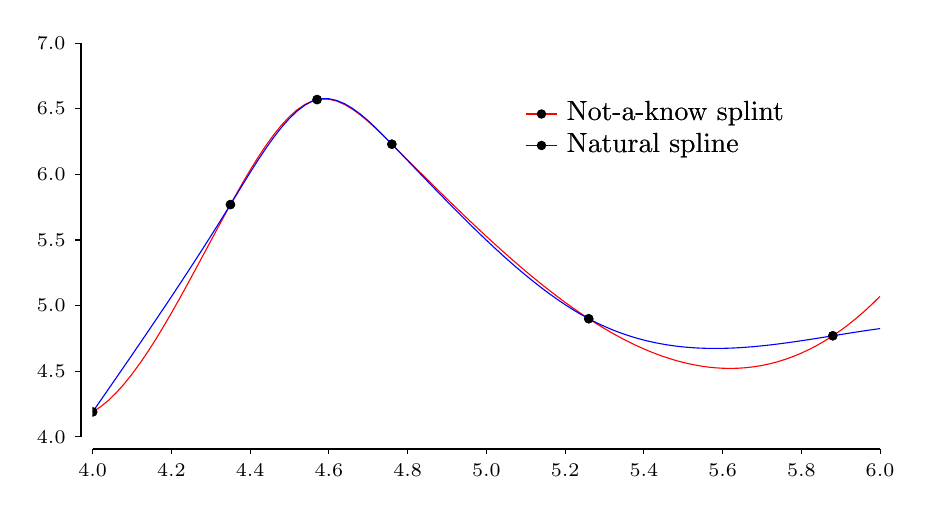
\begin{tikzpicture}[]
\begin{scope}[]
\pgfpathmoveto{ \pgfpointadd{\pgfpointxy {0.0} {0.0}} {\pgfpoint{0cm}{0cm}} }
\pgfpathlineto{ \pgfpointadd{\pgfpointxy {0.0} {0.0}} {\pgfpoint{10cm}{0cm}} }
\pgfpathlineto{ \pgfpointadd{\pgfpointxy {0.0} {0.0}} {\pgfpoint{10cm}{5cm}} }
\pgfpathlineto{ \pgfpointadd{\pgfpointxy {0.0} {0.0}} {\pgfpoint{0cm}{5cm}} }
\pgfpathclose
\pgfusepath{  clip, }
\begin{scope}[shift={(0.0,0.0)}]
\pgfsetxvec{\pgfpoint{5.0cm}{0cm}}
\pgfsetyvec{\pgfpoint{0cm}{1.6666666666666667cm}}
\begin{scope}[shift={(-4.0,-4.0)}]
\begin{scope}[]
\pgfpathmoveto{ \pgfpointadd{\pgfpointxy {4.0} {4.0}} {\pgfpoint{0cm}{0cm}} }
\pgfpathlineto{ \pgfpointadd{\pgfpointxy {4.0} {4.0}} {\pgfpoint{10cm}{0cm}} }
\pgfpathlineto{ \pgfpointadd{\pgfpointxy {4.0} {4.0}} {\pgfpoint{10cm}{5cm}} }
\pgfpathlineto{ \pgfpointadd{\pgfpointxy {4.0} {4.0}} {\pgfpoint{0cm}{5cm}} }
\pgfpathclose
\pgfusepath{  clip, }
\begin{scope}[red]
\pgfpathmoveto{ \pgfpointxy {4.0} {4.19}}
\pgfpathlineto{ \pgfpointxy {4.02} {4.2288933173496535}}
\pgfpathlineto{ \pgfpointxy {4.04} {4.277870024848159}}
\pgfpathlineto{ \pgfpointxy {4.06} {4.336184185327374}}
\pgfpathlineto{ \pgfpointxy {4.08} {4.403089861619165}}
\pgfpathlineto{ \pgfpointxy {4.1} {4.477841116555382}}
\pgfpathlineto{ \pgfpointxy {4.12} {4.559692012967896}}
\pgfpathlineto{ \pgfpointxy {4.14} {4.647896613688557}}
\pgfpathlineto{ \pgfpointxy {4.16} {4.741708981549234}}
\pgfpathlineto{ \pgfpointxy {4.18} {4.84038317938178}}
\pgfpathlineto{ \pgfpointxy {4.2} {4.943173270018062}}
\pgfpathlineto{ \pgfpointxy {4.22} {5.049333316289932}}
\pgfpathlineto{ \pgfpointxy {4.24} {5.158117381029259}}
\pgfpathlineto{ \pgfpointxy {4.26} {5.268779527067894}}
\pgfpathlineto{ \pgfpointxy {4.28} {5.380573817237705}}
\pgfpathlineto{ \pgfpointxy {4.3} {5.492754314370545}}
\pgfpathlineto{ \pgfpointxy {4.32} {5.604575081298282}}
\pgfpathlineto{ \pgfpointxy {4.34} {5.715290180852768}}
\pgfpathlineto{ \pgfpointxy {4.36} {5.824144492927248}}
\pgfpathlineto{ \pgfpointxy {4.38} {5.930171689826624}}
\pgfpathlineto{ \pgfpointxy {4.4} {6.032194236267487}}
\pgfpathlineto{ \pgfpointxy {4.42} {6.129025414027786}}
\pgfpathlineto{ \pgfpointxy {4.44} {6.2194785048854895}}
\pgfpathlineto{ \pgfpointxy {4.46} {6.302366790618549}}
\pgfpathlineto{ \pgfpointxy {4.48} {6.376503553004932}}
\pgfpathlineto{ \pgfpointxy {4.5} {6.440702073822589}}
\pgfpathlineto{ \pgfpointxy {4.52} {6.493775634849485}}
\pgfpathlineto{ \pgfpointxy {4.54} {6.53453751786358}}
\pgfpathlineto{ \pgfpointxy {4.5600000000000005} {6.56180100464283}}
\pgfpathlineto{ \pgfpointxy {4.58} {6.574437556572912}}
\pgfpathlineto{ \pgfpointxy {4.6} {6.572656766016991}}
\pgfpathlineto{ \pgfpointxy {4.62} {6.558006356315717}}
\pgfpathlineto{ \pgfpointxy {4.64} {6.532092230417464}}
\pgfpathlineto{ \pgfpointxy {4.66} {6.496520291270597}}
\pgfpathlineto{ \pgfpointxy {4.68} {6.452896441823487}}
\pgfpathlineto{ \pgfpointxy {4.7} {6.402826585024502}}
\pgfpathlineto{ \pgfpointxy {4.72} {6.347916623822015}}
\pgfpathlineto{ \pgfpointxy {4.74} {6.2897724611643895}}
\pgfpathlineto{ \pgfpointxy {4.76} {6.23}}
\pgfpathlineto{ \pgfpointxy {4.78} {6.169948902792082}}
\pgfpathlineto{ \pgfpointxy {4.8} {6.109943870063351}}
\pgfpathlineto{ \pgfpointxy {4.82} {6.050053361851389}}
\pgfpathlineto{ \pgfpointxy {4.84} {5.990345838193781}}
\pgfpathlineto{ \pgfpointxy {4.86} {5.9308897591281085}}
\pgfpathlineto{ \pgfpointxy {4.88} {5.871753584691959}}
\pgfpathlineto{ \pgfpointxy {4.9} {5.813005774922911}}
\pgfpathlineto{ \pgfpointxy {4.92} {5.754714789858553}}
\pgfpathlineto{ \pgfpointxy {4.94} {5.696949089536464}}
\pgfpathlineto{ \pgfpointxy {4.96} {5.639777133994231}}
\pgfpathlineto{ \pgfpointxy {4.98} {5.583267383269433}}
\pgfpathlineto{ \pgfpointxy {5.0} {5.5274882973996595}}
\pgfpathlineto{ \pgfpointxy {5.02} {5.47250833642249}}
\pgfpathlineto{ \pgfpointxy {5.04} {5.418395960375507}}
\pgfpathlineto{ \pgfpointxy {5.0600000000000005} {5.365219629296296}}
\pgfpathlineto{ \pgfpointxy {5.08} {5.3130478032224415}}
\pgfpathlineto{ \pgfpointxy {5.1} {5.261948942191526}}
\pgfpathlineto{ \pgfpointxy {5.12} {5.21199150624113}}
\pgfpathlineto{ \pgfpointxy {5.140000000000001} {5.1632439554088405}}
\pgfpathlineto{ \pgfpointxy {5.16} {5.115774749732242}}
\pgfpathlineto{ \pgfpointxy {5.18} {5.069652349248916}}
\pgfpathlineto{ \pgfpointxy {5.2} {5.0249452139964434}}
\pgfpathlineto{ \pgfpointxy {5.22} {4.9817218040124125}}
\pgfpathlineto{ \pgfpointxy {5.24} {4.940050579334401}}
\pgfpathlineto{ \pgfpointxy {5.26} {4.9}}
\pgfpathlineto{ \pgfpointxy {5.28} {4.861636317658478}}
\pgfpathlineto{ \pgfpointxy {5.3} {4.8250169504058755}}
\pgfpathlineto{ \pgfpointxy {5.32} {4.790197107949918}}
\pgfpathlineto{ \pgfpointxy {5.34} {4.757231999998338}}
\pgfpathlineto{ \pgfpointxy {5.36} {4.726176836258861}}
\pgfpathlineto{ \pgfpointxy {5.38} {4.697086826439219}}
\pgfpathlineto{ \pgfpointxy {5.4} {4.670017180247137}}
\pgfpathlineto{ \pgfpointxy {5.42} {4.645023107390346}}
\pgfpathlineto{ \pgfpointxy {5.4399999999999995} {4.622159817576572}}
\pgfpathlineto{ \pgfpointxy {5.46} {4.601482520513546}}
\pgfpathlineto{ \pgfpointxy {5.48} {4.583046425908996}}
\pgfpathlineto{ \pgfpointxy {5.5} {4.566906743470651}}
\pgfpathlineto{ \pgfpointxy {5.52} {4.55311868290624}}
\pgfpathlineto{ \pgfpointxy {5.54} {4.5417374539234885}}
\pgfpathlineto{ \pgfpointxy {5.5600000000000005} {4.532818266230128}}
\pgfpathlineto{ \pgfpointxy {5.58} {4.5264163295338875}}
\pgfpathlineto{ \pgfpointxy {5.6} {4.522586853542495}}
\pgfpathlineto{ \pgfpointxy {5.62} {4.521385047963677}}
\pgfpathlineto{ \pgfpointxy {5.640000000000001} {4.522866122505165}}
\pgfpathlineto{ \pgfpointxy {5.66} {4.527085286874686}}
\pgfpathlineto{ \pgfpointxy {5.68} {4.534097750779969}}
\pgfpathlineto{ \pgfpointxy {5.7} {4.543958723928742}}
\pgfpathlineto{ \pgfpointxy {5.72} {4.556723416028735}}
\pgfpathlineto{ \pgfpointxy {5.74} {4.572447036787675}}
\pgfpathlineto{ \pgfpointxy {5.76} {4.591184795913292}}
\pgfpathlineto{ \pgfpointxy {5.78} {4.612991903113314}}
\pgfpathlineto{ \pgfpointxy {5.8} {4.637923568095469}}
\pgfpathlineto{ \pgfpointxy {5.82} {4.666035000567487}}
\pgfpathlineto{ \pgfpointxy {5.84} {4.697381410237095}}
\pgfpathlineto{ \pgfpointxy {5.86} {4.732018006812025}}
\pgfpathlineto{ \pgfpointxy {5.88} {4.77}}
\pgfpathlineto{ \pgfpointxy {5.9} {4.811382599508753}}
\pgfpathlineto{ \pgfpointxy {5.92} {4.85622101504601}}
\pgfpathlineto{ \pgfpointxy {5.9399999999999995} {4.904570456319501}}
\pgfpathlineto{ \pgfpointxy {5.96} {4.9564861330369565}}
\pgfpathlineto{ \pgfpointxy {5.98} {5.0120232549061035}}
\pgfpathlineto{ \pgfpointxy {6.0} {5.071237031634667}}
\pgfusepath{ stroke, }
\end{scope}
\end{scope}
\begin{scope}[]
\pgfpathmoveto{ \pgfpointadd{\pgfpointxy {4.0} {4.0}} {\pgfpoint{0cm}{0cm}} }
\pgfpathlineto{ \pgfpointadd{\pgfpointxy {4.0} {4.0}} {\pgfpoint{10cm}{0cm}} }
\pgfpathlineto{ \pgfpointadd{\pgfpointxy {4.0} {4.0}} {\pgfpoint{10cm}{5cm}} }
\pgfpathlineto{ \pgfpointadd{\pgfpointxy {4.0} {4.0}} {\pgfpoint{0cm}{5cm}} }
\pgfpathclose
\pgfusepath{  clip, }
\node at (4.0,4.19) [fill=black,draw=black,circle,inner sep=0.0pt,minimum width =3.0pt,minimum height=3.0pt] {};
\node at (4.35,5.77) [fill=black,draw=black,circle,inner sep=0.0pt,minimum width =3.0pt,minimum height=3.0pt] {};
\node at (4.57,6.57) [fill=black,draw=black,circle,inner sep=0.0pt,minimum width =3.0pt,minimum height=3.0pt] {};
\node at (4.76,6.23) [fill=black,draw=black,circle,inner sep=0.0pt,minimum width =3.0pt,minimum height=3.0pt] {};
\node at (5.26,4.9) [fill=black,draw=black,circle,inner sep=0.0pt,minimum width =3.0pt,minimum height=3.0pt] {};
\node at (5.88,4.77) [fill=black,draw=black,circle,inner sep=0.0pt,minimum width =3.0pt,minimum height=3.0pt] {};
\end{scope}
\end{scope}
\end{scope}
\pgfsetxvec{\pgfpoint{1cm}{0cm}}
\pgfsetyvec{\pgfpoint{0cm}{1cm}}
\end{scope}
\draw[red] (5.5,4.1) -- (5.9,4.1);
\draw[opacity=0.0,white] (5.5,4.2) -- (5.5,4.0);
\node at (5.9,4.1) [right,] {Not-a-know splint};
\node at (5.7,4.1) [fill=black,draw=black,circle,inner sep=0.0pt,minimum width =3.0pt,minimum height=3.0pt] {};
\node at (5.9,4.1) [right,] {Not-a-know splint};
\begin{scope}[]
\pgfpathmoveto{ \pgfpointadd{\pgfpointxy {0.0} {0.0}} {\pgfpoint{0cm}{0cm}} }
\pgfpathlineto{ \pgfpointadd{\pgfpointxy {0.0} {0.0}} {\pgfpoint{10cm}{0cm}} }
\pgfpathlineto{ \pgfpointadd{\pgfpointxy {0.0} {0.0}} {\pgfpoint{10cm}{5cm}} }
\pgfpathlineto{ \pgfpointadd{\pgfpointxy {0.0} {0.0}} {\pgfpoint{0cm}{5cm}} }
\pgfpathclose
\pgfusepath{  clip, }
\begin{scope}[shift={(0.0,0.0)}]
\pgfsetxvec{\pgfpoint{5.0cm}{0cm}}
\pgfsetyvec{\pgfpoint{0cm}{1.6666666666666667cm}}
\begin{scope}[shift={(-4.0,-4.0)}]
\begin{scope}[]
\pgfpathmoveto{ \pgfpointadd{\pgfpointxy {4.0} {4.0}} {\pgfpoint{0cm}{0cm}} }
\pgfpathlineto{ \pgfpointadd{\pgfpointxy {4.0} {4.0}} {\pgfpoint{10cm}{0cm}} }
\pgfpathlineto{ \pgfpointadd{\pgfpointxy {4.0} {4.0}} {\pgfpoint{10cm}{5cm}} }
\pgfpathlineto{ \pgfpointadd{\pgfpointxy {4.0} {4.0}} {\pgfpoint{0cm}{5cm}} }
\pgfpathclose
\pgfusepath{  clip, }
\begin{scope}[blue]
\pgfpathmoveto{ \pgfpointxy {4.0} {4.19}}
\pgfpathlineto{ \pgfpointxy {4.02} {4.27659219042123}}
\pgfpathlineto{ \pgfpointxy {4.04} {4.363256980820145}}
\pgfpathlineto{ \pgfpointxy {4.06} {4.450066971174415}}
\pgfpathlineto{ \pgfpointxy {4.08} {4.537094761461732}}
\pgfpathlineto{ \pgfpointxy {4.1} {4.624412951659764}}
\pgfpathlineto{ \pgfpointxy {4.12} {4.712094141746202}}
\pgfpathlineto{ \pgfpointxy {4.14} {4.800210931698716}}
\pgfpathlineto{ \pgfpointxy {4.16} {4.888835921494997}}
\pgfpathlineto{ \pgfpointxy {4.18} {4.978041711112716}}
\pgfpathlineto{ \pgfpointxy {4.2} {5.067900900529561}}
\pgfpathlineto{ \pgfpointxy {4.22} {5.158486089723204}}
\pgfpathlineto{ \pgfpointxy {4.24} {5.249869878671334}}
\pgfpathlineto{ \pgfpointxy {4.26} {5.342124867351624}}
\pgfpathlineto{ \pgfpointxy {4.28} {5.43532365574176}}
\pgfpathlineto{ \pgfpointxy {4.3} {5.529538843819415}}
\pgfpathlineto{ \pgfpointxy {4.32} {5.624843031562279}}
\pgfpathlineto{ \pgfpointxy {4.34} {5.721308818948022}}
\pgfpathlineto{ \pgfpointxy {4.36} {5.818974279573464}}
\pgfpathlineto{ \pgfpointxy {4.38} {5.917083380275411}}
\pgfpathlineto{ \pgfpointxy {4.4} {6.014085981130691}}
\pgfpathlineto{ \pgfpointxy {4.42} {6.108397415835243}}
\pgfpathlineto{ \pgfpointxy {4.44} {6.198433018085027}}
\pgfpathlineto{ \pgfpointxy {4.46} {6.282608121575982}}
\pgfpathlineto{ \pgfpointxy {4.48} {6.359338060004066}}
\pgfpathlineto{ \pgfpointxy {4.5} {6.427038167065223}}
\pgfpathlineto{ \pgfpointxy {4.52} {6.484123776455401}}
\pgfpathlineto{ \pgfpointxy {4.54} {6.529010221870556}}
\pgfpathlineto{ \pgfpointxy {4.5600000000000005} {6.560112837006632}}
\pgfpathlineto{ \pgfpointxy {4.58} {6.575914836921859}}
\pgfpathlineto{ \pgfpointxy {4.6} {6.576460708006886}}
\pgfpathlineto{ \pgfpointxy {4.62} {6.563356207984786}}
\pgfpathlineto{ \pgfpointxy {4.64} {6.538274975940911}}
\pgfpathlineto{ \pgfpointxy {4.66} {6.502890650960607}}
\pgfpathlineto{ \pgfpointxy {4.68} {6.458876872129232}}
\pgfpathlineto{ \pgfpointxy {4.7} {6.4079072785321305}}
\pgfpathlineto{ \pgfpointxy {4.72} {6.351655509254659}}
\pgfpathlineto{ \pgfpointxy {4.74} {6.291795203382164}}
\pgfpathlineto{ \pgfpointxy {4.76} {6.23}}
\pgfpathlineto{ \pgfpointxy {4.78} {6.16768423115035}}
\pgfpathlineto{ \pgfpointxy {4.8} {6.105225000702742}}
\pgfpathlineto{ \pgfpointxy {4.82} {6.042740105483533}}
\pgfpathlineto{ \pgfpointxy {4.84} {5.98034734231909}}
\pgfpathlineto{ \pgfpointxy {4.86} {5.9181645080357645}}
\pgfpathlineto{ \pgfpointxy {4.88} {5.856309399459924}}
\pgfpathlineto{ \pgfpointxy {4.9} {5.794899813417925}}
\pgfpathlineto{ \pgfpointxy {4.92} {5.734053546736131}}
\pgfpathlineto{ \pgfpointxy {4.94} {5.6738883962408995}}
\pgfpathlineto{ \pgfpointxy {4.96} {5.614522158758593}}
\pgfpathlineto{ \pgfpointxy {4.98} {5.556072631115571}}
\pgfpathlineto{ \pgfpointxy {5.0} {5.498657610138196}}
\pgfpathlineto{ \pgfpointxy {5.02} {5.442394892652826}}
\pgfpathlineto{ \pgfpointxy {5.04} {5.387402275485819}}
\pgfpathlineto{ \pgfpointxy {5.0600000000000005} {5.333797555463539}}
\pgfpathlineto{ \pgfpointxy {5.08} {5.281698529412348}}
\pgfpathlineto{ \pgfpointxy {5.1} {5.231222994158605}}
\pgfpathlineto{ \pgfpointxy {5.12} {5.182488746528666}}
\pgfpathlineto{ \pgfpointxy {5.140000000000001} {5.1356135833488965}}
\pgfpathlineto{ \pgfpointxy {5.16} {5.090715301445657}}
\pgfpathlineto{ \pgfpointxy {5.18} {5.047911697645307}}
\pgfpathlineto{ \pgfpointxy {5.2} {5.007320568774205}}
\pgfpathlineto{ \pgfpointxy {5.22} {4.969059711658713}}
\pgfpathlineto{ \pgfpointxy {5.24} {4.93324692312519}}
\pgfpathlineto{ \pgfpointxy {5.26} {4.9}}
\pgfpathlineto{ \pgfpointxy {5.28} {4.869402678013522}}
\pgfpathlineto{ \pgfpointxy {5.3} {4.8414024485122304}}
\pgfpathlineto{ \pgfpointxy {5.32} {4.815912741746616}}
\pgfpathlineto{ \pgfpointxy {5.34} {4.792846987967176}}
\pgfpathlineto{ \pgfpointxy {5.36} {4.7721186174244}}
\pgfpathlineto{ \pgfpointxy {5.38} {4.753641060368786}}
\pgfpathlineto{ \pgfpointxy {5.4} {4.737327747050826}}
\pgfpathlineto{ \pgfpointxy {5.42} {4.723092107721014}}
\pgfpathlineto{ \pgfpointxy {5.4399999999999995} {4.710847572629844}}
\pgfpathlineto{ \pgfpointxy {5.46} {4.700507572027809}}
\pgfpathlineto{ \pgfpointxy {5.48} {4.691985536165404}}
\pgfpathlineto{ \pgfpointxy {5.5} {4.685194895293122}}
\pgfpathlineto{ \pgfpointxy {5.52} {4.680049079661458}}
\pgfpathlineto{ \pgfpointxy {5.54} {4.676461519520904}}
\pgfpathlineto{ \pgfpointxy {5.5600000000000005} {4.674345645121956}}
\pgfpathlineto{ \pgfpointxy {5.58} {4.6736148867151055}}
\pgfpathlineto{ \pgfpointxy {5.6} {4.674182674550848}}
\pgfpathlineto{ \pgfpointxy {5.62} {4.675962438879676}}
\pgfpathlineto{ \pgfpointxy {5.640000000000001} {4.678867609952086}}
\pgfpathlineto{ \pgfpointxy {5.66} {4.682811618018568}}
\pgfpathlineto{ \pgfpointxy {5.68} {4.687707893329618}}
\pgfpathlineto{ \pgfpointxy {5.7} {4.693469866135731}}
\pgfpathlineto{ \pgfpointxy {5.72} {4.700010966687398}}
\pgfpathlineto{ \pgfpointxy {5.74} {4.707244625235115}}
\pgfpathlineto{ \pgfpointxy {5.76} {4.715084272029376}}
\pgfpathlineto{ \pgfpointxy {5.78} {4.723443337320674}}
\pgfpathlineto{ \pgfpointxy {5.8} {4.732235251359502}}
\pgfpathlineto{ \pgfpointxy {5.82} {4.741373444396355}}
\pgfpathlineto{ \pgfpointxy {5.84} {4.750771346681726}}
\pgfpathlineto{ \pgfpointxy {5.86} {4.7603423884661105}}
\pgfpathlineto{ \pgfpointxy {5.88} {4.77}}
\pgfpathlineto{ \pgfpointxy {5.9} {4.77965761153389}}
\pgfpathlineto{ \pgfpointxy {5.92} {4.789228653318274}}
\pgfpathlineto{ \pgfpointxy {5.9399999999999995} {4.7986265556036445}}
\pgfpathlineto{ \pgfpointxy {5.96} {4.807764748640497}}
\pgfpathlineto{ \pgfpointxy {5.98} {4.816556662679326}}
\pgfpathlineto{ \pgfpointxy {6.0} {4.824915727970623}}
\pgfusepath{ stroke, }
\end{scope}
\end{scope}
\begin{scope}[]
\pgfpathmoveto{ \pgfpointadd{\pgfpointxy {4.0} {4.0}} {\pgfpoint{0cm}{0cm}} }
\pgfpathlineto{ \pgfpointadd{\pgfpointxy {4.0} {4.0}} {\pgfpoint{10cm}{0cm}} }
\pgfpathlineto{ \pgfpointadd{\pgfpointxy {4.0} {4.0}} {\pgfpoint{10cm}{5cm}} }
\pgfpathlineto{ \pgfpointadd{\pgfpointxy {4.0} {4.0}} {\pgfpoint{0cm}{5cm}} }
\pgfpathclose
\pgfusepath{  clip, }
\node at (4.0,4.19) [fill=black,draw=black,circle,inner sep=0.0pt,minimum width =3.0pt,minimum height=3.0pt] {};
\node at (4.35,5.77) [fill=black,draw=black,circle,inner sep=0.0pt,minimum width =3.0pt,minimum height=3.0pt] {};
\node at (4.57,6.57) [fill=black,draw=black,circle,inner sep=0.0pt,minimum width =3.0pt,minimum height=3.0pt] {};
\node at (4.76,6.23) [fill=black,draw=black,circle,inner sep=0.0pt,minimum width =3.0pt,minimum height=3.0pt] {};
\node at (5.26,4.9) [fill=black,draw=black,circle,inner sep=0.0pt,minimum width =3.0pt,minimum height=3.0pt] {};
\node at (5.88,4.77) [fill=black,draw=black,circle,inner sep=0.0pt,minimum width =3.0pt,minimum height=3.0pt] {};
\end{scope}
\end{scope}
\end{scope}
\pgfsetxvec{\pgfpoint{1cm}{0cm}}
\pgfsetyvec{\pgfpoint{0cm}{1cm}}
\end{scope}
\draw[blue] (5.5,3.7) -- (5.9,3.7);
\draw[opacity=0.0,white] (5.5,3.8000000000000003) -- (5.5,3.6);
\node at (5.9,3.7) [right,] {Natural spline};
\node at (5.7,3.7) [fill=black,draw=black,circle,inner sep=0.0pt,minimum width =3.0pt,minimum height=3.0pt] {};
\node at (5.9,3.7) [right,] {Natural spline};
\begin{scope}[shift={(0.0,0.0)}]
\pgfsetxvec{\pgfpoint{5.0cm}{0cm}}
\pgfsetyvec{\pgfpoint{0cm}{1.6666666666666667cm}}
\begin{scope}[shift={(-4.0,-4.0)}]
\begin{scope}[thick,black,fill=white]
\pgfpathmoveto{ \pgfpointadd{\pgfpointxy {4.0} {4.0}} {\pgfpoint{0}{-0.15cm}} }
\pgfpathlineto{ \pgfpointadd{\pgfpointxy {6.0} {4.0}} {\pgfpoint{0}{-0.15cm}} }
\pgfpathmoveto{ \pgfpointadd{\pgfpointxy {4.0} {4.0}} {\pgfpoint{-0.15cm}{0}} }
\pgfpathlineto{ \pgfpointadd{\pgfpointxy {4.0} {7.0}} {\pgfpoint{-0.15cm}{0}} }
\pgfusepath{ stroke, }
\end{scope}
\begin{scope}[yshift=-0.15cm]
\draw[] [shift={(4.0,4.0)}] (0,0) -- (0,-2pt) node[below]{ \scriptsize{\num[round-mode=places,round-precision=1]{4.0}}};
\draw[] [shift={(4.2,4.0)}] (0,0) -- (0,-2pt) node[below]{ \scriptsize{\num[round-mode=places,round-precision=1]{4.2}}};
\draw[] [shift={(4.4,4.0)}] (0,0) -- (0,-2pt) node[below]{ \scriptsize{\num[round-mode=places,round-precision=1]{4.4}}};
\draw[] [shift={(4.6,4.0)}] (0,0) -- (0,-2pt) node[below]{ \scriptsize{\num[round-mode=places,round-precision=1]{4.6}}};
\draw[] [shift={(4.8,4.0)}] (0,0) -- (0,-2pt) node[below]{ \scriptsize{\num[round-mode=places,round-precision=1]{4.8}}};
\draw[] [shift={(5.0,4.0)}] (0,0) -- (0,-2pt) node[below]{ \scriptsize{\num[round-mode=places,round-precision=1]{5.0}}};
\draw[] [shift={(5.2,4.0)}] (0,0) -- (0,-2pt) node[below]{ \scriptsize{\num[round-mode=places,round-precision=1]{5.2}}};
\draw[] [shift={(5.4,4.0)}] (0,0) -- (0,-2pt) node[below]{ \scriptsize{\num[round-mode=places,round-precision=1]{5.4}}};
\draw[] [shift={(5.6,4.0)}] (0,0) -- (0,-2pt) node[below]{ \scriptsize{\num[round-mode=places,round-precision=1]{5.6}}};
\draw[] [shift={(5.8,4.0)}] (0,0) -- (0,-2pt) node[below]{ \scriptsize{\num[round-mode=places,round-precision=1]{5.8}}};
\draw[] [shift={(6.0,4.0)}] (0,0) -- (0,-2pt) node[below]{ \scriptsize{\num[round-mode=places,round-precision=1]{6.0}}};
\end{scope}
\begin{scope}[xshift=-0.15cm]
\draw[] [shift={(4.0,4.0)}] (0,0) -- (-2pt,0) node[left]{ \scriptsize{\num[round-mode=places,round-precision=1]{4.0}}};
\draw[] [shift={(4.0,4.5)}] (0,0) -- (-2pt,0) node[left]{ \scriptsize{\num[round-mode=places,round-precision=1]{4.5}}};
\draw[] [shift={(4.0,5.0)}] (0,0) -- (-2pt,0) node[left]{ \scriptsize{\num[round-mode=places,round-precision=1]{5.0}}};
\draw[] [shift={(4.0,5.5)}] (0,0) -- (-2pt,0) node[left]{ \scriptsize{\num[round-mode=places,round-precision=1]{5.5}}};
\draw[] [shift={(4.0,6.0)}] (0,0) -- (-2pt,0) node[left]{ \scriptsize{\num[round-mode=places,round-precision=1]{6.0}}};
\draw[] [shift={(4.0,6.5)}] (0,0) -- (-2pt,0) node[left]{ \scriptsize{\num[round-mode=places,round-precision=1]{6.5}}};
\draw[] [shift={(4.0,7.0)}] (0,0) -- (-2pt,0) node[left]{ \scriptsize{\num[round-mode=places,round-precision=1]{7.0}}};
\end{scope}
\end{scope}
\end{scope}
\pgfsetxvec{\pgfpoint{1cm}{0cm}}
\pgfsetyvec{\pgfpoint{0cm}{1cm}}
\end{tikzpicture}
\end{document}

  \caption{Comparison of splines with different end point conditions.}
\end{figure}

\begin{figure}[H]
  \centering
  \documentclass{standalone}
\ifx\HCode\UnDef\else\def\pgfsysdriver{pgfsys-tex4ht.def}\fi
\usepackage{tikz}
\usepackage{color}
\usepackage{siunitx}
\usetikzlibrary{arrows,shapes}
\begin{document}
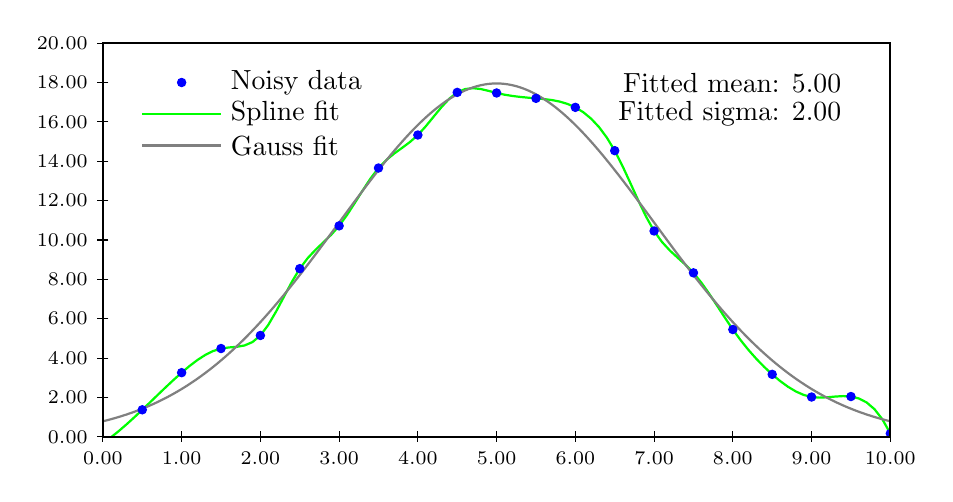
\begin{tikzpicture}
\begin{scope}[]
\pgfpathmoveto{ \pgfpointxy {0.0} {0.0}}
\pgfpathlineto{ \pgfpointxy {10.0} {0.0}}
\pgfpathlineto{ \pgfpointxy {10.0} {5.0}}
\pgfpathlineto{ \pgfpointxy {0.0} {5.0}}
\pgfpathclose
\pgfusepath{  clip, }
\begin{scope}[shift={(0.0,0.0)}]
\pgfsetxvec{\pgfpoint{1.0cm}{0cm}}
\pgfsetyvec{\pgfpoint{0cm}{0.25cm}}
\begin{scope}[shift={(0.0,0.0)}]
\begin{scope}[green,thick]
\pgfpathmoveto{ \pgfpointxy {0.0} {-0.3220822684578466}}
\pgfpathlineto{ \pgfpointxy {0.1} {-0.03179540914739956}}
\pgfpathlineto{ \pgfpointxy {0.2} {0.2885428151650948}}
\pgfpathlineto{ \pgfpointxy {0.3} {0.633328152486329}}
\pgfpathlineto{ \pgfpointxy {0.4} {0.9969563508229966}}
\pgfpathlineto{ \pgfpointxy {0.5} {1.3738231581817897}}
\pgfpathlineto{ \pgfpointxy {0.6} {1.7583243225694014}}
\pgfpathlineto{ \pgfpointxy {0.7} {2.144855591992525}}
\pgfpathlineto{ \pgfpointxy {0.8} {2.5278127144578533}}
\pgfpathlineto{ \pgfpointxy {0.9} {2.9015914379720784}}
\pgfpathlineto{ \pgfpointxy {1.0} {3.2605875105418933}}
\pgfpathlineto{ \pgfpointxy {1.1} {3.59798429165626}}
\pgfpathlineto{ \pgfpointxy {1.2} {3.9021155867332062}}
\pgfpathlineto{ \pgfpointxy {1.3} {4.160102812673034}}
\pgfpathlineto{ \pgfpointxy {1.4} {4.359067386376038}}
\pgfpathlineto{ \pgfpointxy {1.5} {4.486130724742518}}
\pgfpathlineto{ \pgfpointxy {1.6} {4.540874002276166}}
\pgfpathlineto{ \pgfpointxy {1.7} {4.572717423894254}}
\pgfpathlineto{ \pgfpointxy {1.8} {4.6435409521174424}}
\pgfpathlineto{ \pgfpointxy {1.9} {4.815224549466396}}
\pgfpathlineto{ \pgfpointxy {2.0} {5.149648178461778}}
\pgfpathlineto{ \pgfpointxy {2.1} {5.685601299272113}}
\pgfpathlineto{ \pgfpointxy {2.2} {6.3695113626573665}}
\pgfpathlineto{ \pgfpointxy {2.3} {7.124715317025358}}
\pgfpathlineto{ \pgfpointxy {2.4} {7.874550110783923}}
\pgfpathlineto{ \pgfpointxy {2.5} {8.54235269234088}}
\pgfpathlineto{ \pgfpointxy {2.6} {9.073464969531473}}
\pgfpathlineto{ \pgfpointxy {2.7} {9.50124868790061}}
\pgfpathlineto{ \pgfpointxy {2.8} {9.88107055242061}}
\pgfpathlineto{ \pgfpointxy {2.9} {10.268297268063803}}
\pgfpathlineto{ \pgfpointxy {3.0} {10.718295539802511}}
\pgfpathlineto{ \pgfpointxy {3.1} {11.268900377785958}}
\pgfpathlineto{ \pgfpointxy {3.2} {11.887820012870971}}
\pgfpathlineto{ \pgfpointxy {3.3} {12.52523098109127}}
\pgfpathlineto{ \pgfpointxy {3.4} {13.131309818480585}}
\pgfpathlineto{ \pgfpointxy {3.5} {13.656233061072639}}
\pgfpathlineto{ \pgfpointxy {3.6} {14.066283096326574}}
\pgfpathlineto{ \pgfpointxy {3.7} {14.392165717403207}}
\pgfpathlineto{ \pgfpointxy {3.8} {14.680692568888766}}
\pgfpathlineto{ \pgfpointxy {3.9} {14.978675295369484}}
\pgfpathlineto{ \pgfpointxy {4.0} {15.3329255414316}}
\pgfpathlineto{ \pgfpointxy {4.1} {15.773545607044694}}
\pgfpathlineto{ \pgfpointxy {4.2} {16.263800413711795}}
\pgfpathlineto{ \pgfpointxy {4.3} {16.75024553831928}}
\pgfpathlineto{ \pgfpointxy {4.4} {17.179436557753533}}
\pgfpathlineto{ \pgfpointxy {4.5} {17.497929048900925}}
\pgfpathlineto{ \pgfpointxy {4.6} {17.667544878429773}}
\pgfpathlineto{ \pgfpointxy {4.7} {17.711171072136075}}
\pgfpathlineto{ \pgfpointxy {4.8} {17.666960945597783}}
\pgfpathlineto{ \pgfpointxy {4.9} {17.57306781439283}}
\pgfpathlineto{ \pgfpointxy {5.0} {17.46764499409915}}
\pgfpathlineto{ \pgfpointxy {5.1} {17.38158457781227}}
\pgfpathlineto{ \pgfpointxy {5.2} {17.31673376869809}}
\pgfpathlineto{ \pgfpointxy {5.3} {17.267678547440084}}
\pgfpathlineto{ \pgfpointxy {5.4} {17.22900489472175}}
\pgfpathlineto{ \pgfpointxy {5.5} {17.195298791226566}}
\pgfpathlineto{ \pgfpointxy {5.6} {17.15975016321322}}
\pgfpathlineto{ \pgfpointxy {5.7} {17.109964719241223}}
\pgfpathlineto{ \pgfpointxy {5.8} {17.0321521134453}}
\pgfpathlineto{ \pgfpointxy {5.9} {16.912521999960166}}
\pgfpathlineto{ \pgfpointxy {6.0} {16.73728403292054}}
\pgfpathlineto{ \pgfpointxy {6.1} {16.492593096437812}}
\pgfpathlineto{ \pgfpointxy {6.2} {16.164384994530018}}
\pgfpathlineto{ \pgfpointxy {6.3} {15.738540761191885}}
\pgfpathlineto{ \pgfpointxy {6.4} {15.200941430418121}}
\pgfpathlineto{ \pgfpointxy {6.5} {14.537468036203448}}
\pgfpathlineto{ \pgfpointxy {6.6} {13.746955063475587}}
\pgfpathlineto{ \pgfpointxy {6.7} {12.880050800894296}}
\pgfpathlineto{ \pgfpointxy {6.8} {12.000356988052364}}
\pgfpathlineto{ \pgfpointxy {6.9} {11.171475364542555}}
\pgfpathlineto{ \pgfpointxy {7.0} {10.457007669957658}}
\pgfpathlineto{ \pgfpointxy {7.1} {9.900588706936261}}
\pgfpathlineto{ \pgfpointxy {7.2} {9.465985530300243}}
\pgfpathlineto{ \pgfpointxy {7.3} {9.096998257917303}}
\pgfpathlineto{ \pgfpointxy {7.4} {8.737427007655137}}
\pgfpathlineto{ \pgfpointxy {7.5} {8.331071897381452}}
\pgfpathlineto{ \pgfpointxy {7.6} {7.836306153830907}}
\pgfpathlineto{ \pgfpointxy {7.7} {7.269795439206012}}
\pgfpathlineto{ \pgfpointxy {7.8} {6.662778524576263}}
\pgfpathlineto{ \pgfpointxy {7.9} {6.046494181011129}}
\pgfpathlineto{ \pgfpointxy {8.0} {5.452181179580102}}
\pgfpathlineto{ \pgfpointxy {8.1} {4.905237179264141}}
\pgfpathlineto{ \pgfpointxy {8.2} {4.4076953906901215}}
\pgfpathlineto{ \pgfpointxy {8.3} {3.9557479123963915}}
\pgfpathlineto{ \pgfpointxy {8.4} {3.545586842921326}}
\pgfpathlineto{ \pgfpointxy {8.5} {3.173404280803272}}
\pgfpathlineto{ \pgfpointxy {8.6} {2.837587185462304}}
\pgfpathlineto{ \pgfpointxy {8.7} {2.545301959845368}}
\pgfpathlineto{ \pgfpointxy {8.8} {2.305909867781125}}
\pgfpathlineto{ \pgfpointxy {8.9} {2.128772173098246}}
\pgfpathlineto{ \pgfpointxy {9.0} {2.0232501396253917}}
\pgfpathlineto{ \pgfpointxy {9.1} {1.9919084111773382}}
\pgfpathlineto{ \pgfpointxy {9.2} {2.010125151513315}}
\pgfpathlineto{ \pgfpointxy {9.3} {2.046481904378665}}
\pgfpathlineto{ \pgfpointxy {9.4} {2.0695602135187294}}
\pgfpathlineto{ \pgfpointxy {9.5} {2.047941622678851}}
\pgfpathlineto{ \pgfpointxy {9.6} {1.9502076756043718}}
\pgfpathlineto{ \pgfpointxy {9.7} {1.744939916040635}}
\pgfpathlineto{ \pgfpointxy {9.8} {1.400719887732975}}
\pgfpathlineto{ \pgfpointxy {9.9} {0.8861291344267457}}
\pgfpathlineto{ \pgfpointxy {10.0} {0.16974919986728543}}
\pgfusepath{ stroke, }
\end{scope}
\begin{scope}[thick,gray]
\pgfpathmoveto{ \pgfpointxy {0.0} {0.7887735222102034}}
\pgfpathlineto{ \pgfpointxy {0.05} {0.8393826956517481}}
\pgfpathlineto{ \pgfpointxy {0.1} {0.892680947630374}}
\pgfpathlineto{ \pgfpointxy {0.15} {0.9487703099544526}}
\pgfpathlineto{ \pgfpointxy {0.2} {1.0077538632674794}}
\pgfpathlineto{ \pgfpointxy {0.25} {1.0697355373456514}}
\pgfpathlineto{ \pgfpointxy {0.3} {1.134819896183258}}
\pgfpathlineto{ \pgfpointxy {0.35} {1.203111907750662}}
\pgfpathlineto{ \pgfpointxy {0.4} {1.2747166983715252}}
\pgfpathlineto{ \pgfpointxy {0.45} {1.3497392917319906}}
\pgfpathlineto{ \pgfpointxy {0.5} {1.4282843326044656}}
\pgfpathlineto{ \pgfpointxy {0.55} {1.5104557954424003}}
\pgfpathlineto{ \pgfpointxy {0.6} {1.5963566780798044}}
\pgfpathlineto{ \pgfpointxy {0.65} {1.6860886808498898}}
\pgfpathlineto{ \pgfpointxy {0.7} {1.779751871521008}}
\pgfpathlineto{ \pgfpointxy {0.75} {1.8774443365345639}}
\pgfpathlineto{ \pgfpointxy {0.8} {1.9792618191185283}}
\pgfpathlineto{ \pgfpointxy {0.85} {2.0852973449411976}}
\pgfpathlineto{ \pgfpointxy {0.9} {2.1956408360624864}}
\pgfpathlineto{ \pgfpointxy {0.95} {2.310378714033865}}
\pgfpathlineto{ \pgfpointxy {1.0} {2.42959349309268}}
\pgfpathlineto{ \pgfpointxy {1.05} {2.5533633644912777}}
\pgfpathlineto{ \pgfpointxy {1.1} {2.6817617730958987}}
\pgfpathlineto{ \pgfpointxy {1.15} {2.8148569874838527}}
\pgfpathlineto{ \pgfpointxy {1.2} {2.95271166485958}}
\pgfpathlineto{ \pgfpointxy {1.25} {3.0953824122002476}}
\pgfpathlineto{ \pgfpointxy {1.3} {3.2429193451289016}}
\pgfpathlineto{ \pgfpointxy {1.35} {3.3953656460971313}}
\pgfpathlineto{ \pgfpointxy {1.4} {3.5527571235392896}}
\pgfpathlineto{ \pgfpointxy {1.45} {3.7151217737356554}}
\pgfpathlineto{ \pgfpointxy {1.5} {3.882479347192031}}
\pgfpathlineto{ \pgfpointxy {1.55} {4.0548409214074095}}
\pgfpathlineto{ \pgfpointxy {1.6} {4.232208481958889}}
\pgfpathlineto{ \pgfpointxy {1.65} {4.414574513883361}}
\pgfpathlineto{ \pgfpointxy {1.7} {4.601921605377953}}
\pgfpathlineto{ \pgfpointxy {1.75} {4.794222065875254}}
\pgfpathlineto{ \pgfpointxy {1.8} {4.991437560574411}}
\pgfpathlineto{ \pgfpointxy {1.85} {5.193518763524646}}
\pgfpathlineto{ \pgfpointxy {1.9} {5.400405031363236}}
\pgfpathlineto{ \pgfpointxy {1.95} {5.612024099804946}}
\pgfpathlineto{ \pgfpointxy {2.0} {5.828291804963986}}
\pgfpathlineto{ \pgfpointxy {2.05} {6.0491118315624055}}
\pgfpathlineto{ \pgfpointxy {2.1} {6.27437549004005}}
\pgfpathlineto{ \pgfpointxy {2.15} {6.503961524530807}}
\pgfpathlineto{ \pgfpointxy {2.2} {6.7377359536073405}}
\pgfpathlineto{ \pgfpointxy {2.25} {6.975551945622008}}
\pgfpathlineto{ \pgfpointxy {2.3} {7.217249730385189}}
\pgfpathlineto{ \pgfpointxy {2.35} {7.462656548823516}}
\pgfpathlineto{ \pgfpointxy {2.4} {7.71158664215013}}
\pgfpathlineto{ \pgfpointxy {2.45} {7.963841281956886}}
\pgfpathlineto{ \pgfpointxy {2.5} {8.219208842504782}}
\pgfpathlineto{ \pgfpointxy {2.55} {8.47746491634448}}
\pgfpathlineto{ \pgfpointxy {2.6} {8.73837247424338}}
\pgfpathlineto{ \pgfpointxy {2.65} {9.001682070230748}}
\pgfpathlineto{ \pgfpointxy {2.7} {9.267132092397667}}
\pgfpathlineto{ \pgfpointxy {2.75} {9.534449059905283}}
\pgfpathlineto{ \pgfpointxy {2.8} {9.803347966463585}}
\pgfpathlineto{ \pgfpointxy {2.85} {10.073532670344598}}
\pgfpathlineto{ \pgfpointxy {2.9} {10.344696330789311}}
\pgfpathlineto{ \pgfpointxy {2.95} {10.6165218904581}}
\pgfpathlineto{ \pgfpointxy {3.0} {10.888682603360296}}
\pgfpathlineto{ \pgfpointxy {3.05} {11.160842607482026}}
\pgfpathlineto{ \pgfpointxy {3.1} {11.432657541112373}}
\pgfpathlineto{ \pgfpointxy {3.15} {11.703775201648687}}
\pgfpathlineto{ \pgfpointxy {3.2} {11.973836245442861}}
\pgfpathlineto{ \pgfpointxy {3.25} {12.242474927033365}}
\pgfpathlineto{ \pgfpointxy {3.3} {12.509319875893764}}
\pgfpathlineto{ \pgfpointxy {3.35} {12.773994908618867}}
\pgfpathlineto{ \pgfpointxy {3.4} {13.036119874265678}}
\pgfpathlineto{ \pgfpointxy {3.45} {13.295311530369304}}
\pgfpathlineto{ \pgfpointxy {3.5} {13.551184446965188}}
\pgfpathlineto{ \pgfpointxy {3.55} {13.803351935769804}}
\pgfpathlineto{ \pgfpointxy {3.6} {14.051427001503281}}
\pgfpathlineto{ \pgfpointxy {3.65} {14.295023312180714}}
\pgfpathlineto{ \pgfpointxy {3.7} {14.533756185055205}}
\pgfpathlineto{ \pgfpointxy {3.75} {14.767243584765959}}
\pgfpathlineto{ \pgfpointxy {3.8} {14.995107130130082}}
\pgfpathlineto{ \pgfpointxy {3.85} {15.216973105918132}}
\pgfpathlineto{ \pgfpointxy {3.9} {15.432473475871411}}
\pgfpathlineto{ \pgfpointxy {3.95} {15.64124689315482}}
\pgfpathlineto{ \pgfpointxy {4.0} {15.84293970439265}}
\pgfpathlineto{ \pgfpointxy {4.05} {16.037206943407437}}
\pgfpathlineto{ \pgfpointxy {4.1} {16.223713310773366}}
\pgfpathlineto{ \pgfpointxy {4.15} {16.40213413530702}}
\pgfpathlineto{ \pgfpointxy {4.2} {16.572156313648794}}
\pgfpathlineto{ \pgfpointxy {4.25} {16.73347922413886}}
\pgfpathlineto{ \pgfpointxy {4.3} {16.885815611261478}}
\pgfpathlineto{ \pgfpointxy {4.35} {17.028892437021163}}
\pgfpathlineto{ \pgfpointxy {4.4} {17.162451695722886}}
\pgfpathlineto{ \pgfpointxy {4.45} {17.28625118875603}}
\pgfpathlineto{ \pgfpointxy {4.5} {17.40006525612754}}
\pgfpathlineto{ \pgfpointxy {4.55} {17.503685461653063}}
\pgfpathlineto{ \pgfpointxy {4.6} {17.596921228894864}}
\pgfpathlineto{ \pgfpointxy {4.65} {17.679600425131426}}
\pgfpathlineto{ \pgfpointxy {4.7} {17.751569890854366}}
\pgfpathlineto{ \pgfpointxy {4.75} {17.8126959125131}}
\pgfpathlineto{ \pgfpointxy {4.8} {17.862864636464906}}
\pgfpathlineto{ \pgfpointxy {4.85} {17.90198242233675}}
\pgfpathlineto{ \pgfpointxy {4.9} {17.929976134263764}}
\pgfpathlineto{ \pgfpointxy {4.95} {17.946793368736568}}
\pgfpathlineto{ \pgfpointxy {5.0} {17.952402618063857}}
\pgfpathlineto{ \pgfpointxy {5.05} {17.946793368736568}}
\pgfpathlineto{ \pgfpointxy {5.1} {17.929976134263764}}
\pgfpathlineto{ \pgfpointxy {5.15} {17.90198242233675}}
\pgfpathlineto{ \pgfpointxy {5.2} {17.862864636464906}}
\pgfpathlineto{ \pgfpointxy {5.25} {17.8126959125131}}
\pgfpathlineto{ \pgfpointxy {5.3} {17.751569890854366}}
\pgfpathlineto{ \pgfpointxy {5.35} {17.679600425131426}}
\pgfpathlineto{ \pgfpointxy {5.4} {17.596921228894864}}
\pgfpathlineto{ \pgfpointxy {5.45} {17.503685461653063}}
\pgfpathlineto{ \pgfpointxy {5.5} {17.40006525612754}}
\pgfpathlineto{ \pgfpointxy {5.55} {17.28625118875603}}
\pgfpathlineto{ \pgfpointxy {5.6} {17.162451695722886}}
\pgfpathlineto{ \pgfpointxy {5.65} {17.028892437021163}}
\pgfpathlineto{ \pgfpointxy {5.7} {16.885815611261478}}
\pgfpathlineto{ \pgfpointxy {5.75} {16.73347922413886}}
\pgfpathlineto{ \pgfpointxy {5.8} {16.572156313648794}}
\pgfpathlineto{ \pgfpointxy {5.85} {16.40213413530702}}
\pgfpathlineto{ \pgfpointxy {5.9} {16.223713310773366}}
\pgfpathlineto{ \pgfpointxy {5.95} {16.037206943407437}}
\pgfpathlineto{ \pgfpointxy {6.0} {15.84293970439265}}
\pgfpathlineto{ \pgfpointxy {6.05} {15.64124689315482}}
\pgfpathlineto{ \pgfpointxy {6.1} {15.432473475871413}}
\pgfpathlineto{ \pgfpointxy {6.15} {15.21697310591813}}
\pgfpathlineto{ \pgfpointxy {6.2} {14.995107130130082}}
\pgfpathlineto{ \pgfpointxy {6.25} {14.767243584765959}}
\pgfpathlineto{ \pgfpointxy {6.3} {14.533756185055205}}
\pgfpathlineto{ \pgfpointxy {6.35} {14.295023312180716}}
\pgfpathlineto{ \pgfpointxy {6.4} {14.05142700150328}}
\pgfpathlineto{ \pgfpointxy {6.45} {13.803351935769804}}
\pgfpathlineto{ \pgfpointxy {6.5} {13.551184446965188}}
\pgfpathlineto{ \pgfpointxy {6.55} {13.295311530369304}}
\pgfpathlineto{ \pgfpointxy {6.6} {13.03611987426568}}
\pgfpathlineto{ \pgfpointxy {6.65} {12.773994908618866}}
\pgfpathlineto{ \pgfpointxy {6.7} {12.509319875893764}}
\pgfpathlineto{ \pgfpointxy {6.75} {12.242474927033365}}
\pgfpathlineto{ \pgfpointxy {6.8} {11.973836245442861}}
\pgfpathlineto{ \pgfpointxy {6.85} {11.70377520164869}}
\pgfpathlineto{ \pgfpointxy {6.9} {11.43265754111237}}
\pgfpathlineto{ \pgfpointxy {6.95} {11.160842607482026}}
\pgfpathlineto{ \pgfpointxy {7.0} {10.888682603360296}}
\pgfpathlineto{ \pgfpointxy {7.05} {10.6165218904581}}
\pgfpathlineto{ \pgfpointxy {7.1} {10.344696330789315}}
\pgfpathlineto{ \pgfpointxy {7.15} {10.073532670344594}}
\pgfpathlineto{ \pgfpointxy {7.2} {9.803347966463585}}
\pgfpathlineto{ \pgfpointxy {7.25} {9.534449059905283}}
\pgfpathlineto{ \pgfpointxy {7.3} {9.267132092397667}}
\pgfpathlineto{ \pgfpointxy {7.35} {9.00168207023075}}
\pgfpathlineto{ \pgfpointxy {7.4} {8.738372474243379}}
\pgfpathlineto{ \pgfpointxy {7.45} {8.47746491634448}}
\pgfpathlineto{ \pgfpointxy {7.5} {8.219208842504782}}
\pgfpathlineto{ \pgfpointxy {7.55} {7.963841281956886}}
\pgfpathlineto{ \pgfpointxy {7.6} {7.711586642150132}}
\pgfpathlineto{ \pgfpointxy {7.65} {7.462656548823513}}
\pgfpathlineto{ \pgfpointxy {7.7} {7.217249730385189}}
\pgfpathlineto{ \pgfpointxy {7.75} {6.975551945622008}}
\pgfpathlineto{ \pgfpointxy {7.8} {6.7377359536073405}}
\pgfpathlineto{ \pgfpointxy {7.85} {6.503961524530809}}
\pgfpathlineto{ \pgfpointxy {7.9} {6.274375490040049}}
\pgfpathlineto{ \pgfpointxy {7.95} {6.0491118315624055}}
\pgfpathlineto{ \pgfpointxy {8.0} {5.828291804963986}}
\pgfpathlineto{ \pgfpointxy {8.05} {5.612024099804942}}
\pgfpathlineto{ \pgfpointxy {8.1} {5.4004050313632375}}
\pgfpathlineto{ \pgfpointxy {8.15} {5.193518763524644}}
\pgfpathlineto{ \pgfpointxy {8.2} {4.991437560574414}}
\pgfpathlineto{ \pgfpointxy {8.25} {4.794222065875254}}
\pgfpathlineto{ \pgfpointxy {8.3} {4.60192160537795}}
\pgfpathlineto{ \pgfpointxy {8.35} {4.4145745138833625}}
\pgfpathlineto{ \pgfpointxy {8.4} {4.232208481958887}}
\pgfpathlineto{ \pgfpointxy {8.45} {4.054840921407412}}
\pgfpathlineto{ \pgfpointxy {8.5} {3.882479347192031}}
\pgfpathlineto{ \pgfpointxy {8.55} {3.7151217737356528}}
\pgfpathlineto{ \pgfpointxy {8.6} {3.55275712353929}}
\pgfpathlineto{ \pgfpointxy {8.65} {3.3953656460971304}}
\pgfpathlineto{ \pgfpointxy {8.7} {3.2429193451289042}}
\pgfpathlineto{ \pgfpointxy {8.75} {3.0953824122002476}}
\pgfpathlineto{ \pgfpointxy {8.8} {2.9527116648595775}}
\pgfpathlineto{ \pgfpointxy {8.85} {2.8148569874838545}}
\pgfpathlineto{ \pgfpointxy {8.9} {2.681761773095898}}
\pgfpathlineto{ \pgfpointxy {8.95} {2.55336336449128}}
\pgfpathlineto{ \pgfpointxy {9.0} {2.42959349309268}}
\pgfpathlineto{ \pgfpointxy {9.05} {2.310378714033863}}
\pgfpathlineto{ \pgfpointxy {9.1} {2.1956408360624864}}
\pgfpathlineto{ \pgfpointxy {9.15} {2.0852973449411976}}
\pgfpathlineto{ \pgfpointxy {9.2} {1.97926181911853}}
\pgfpathlineto{ \pgfpointxy {9.25} {1.8774443365345639}}
\pgfpathlineto{ \pgfpointxy {9.3} {1.7797518715210063}}
\pgfpathlineto{ \pgfpointxy {9.35} {1.6860886808498898}}
\pgfpathlineto{ \pgfpointxy {9.4} {1.5963566780798044}}
\pgfpathlineto{ \pgfpointxy {9.45} {1.5104557954424018}}
\pgfpathlineto{ \pgfpointxy {9.5} {1.4282843326044656}}
\pgfpathlineto{ \pgfpointxy {9.55} {1.3497392917319893}}
\pgfpathlineto{ \pgfpointxy {9.6} {1.2747166983715252}}
\pgfpathlineto{ \pgfpointxy {9.65} {1.203111907750662}}
\pgfpathlineto{ \pgfpointxy {9.7} {1.1348198961832596}}
\pgfpathlineto{ \pgfpointxy {9.75} {1.0697355373456514}}
\pgfpathlineto{ \pgfpointxy {9.8} {1.0077538632674785}}
\pgfpathlineto{ \pgfpointxy {9.85} {0.9487703099544526}}
\pgfpathlineto{ \pgfpointxy {9.9} {0.892680947630374}}
\pgfpathlineto{ \pgfpointxy {9.95} {0.8393826956517488}}
\pgfpathlineto{ \pgfpointxy {10.0} {0.7887735222102034}}
\pgfusepath{ stroke, }
\end{scope}
\node at (0.0,-0.3220822684578466) [circle,inner sep=0.0pt,minimum width =3.0pt,minimum height=3.0pt,draw=blue,fill=blue] {}; 
\node at (0.5,1.3738231581817897) [circle,inner sep=0.0pt,minimum width =3.0pt,minimum height=3.0pt,draw=blue,fill=blue] {}; 
\node at (1.0,3.2605875105418933) [circle,inner sep=0.0pt,minimum width =3.0pt,minimum height=3.0pt,draw=blue,fill=blue] {}; 
\node at (1.5,4.486130724742518) [circle,inner sep=0.0pt,minimum width =3.0pt,minimum height=3.0pt,draw=blue,fill=blue] {}; 
\node at (2.0,5.149648178461778) [circle,inner sep=0.0pt,minimum width =3.0pt,minimum height=3.0pt,draw=blue,fill=blue] {}; 
\node at (2.5,8.54235269234088) [circle,inner sep=0.0pt,minimum width =3.0pt,minimum height=3.0pt,draw=blue,fill=blue] {}; 
\node at (3.0,10.718295539802511) [circle,inner sep=0.0pt,minimum width =3.0pt,minimum height=3.0pt,draw=blue,fill=blue] {}; 
\node at (3.5,13.656233061072639) [circle,inner sep=0.0pt,minimum width =3.0pt,minimum height=3.0pt,draw=blue,fill=blue] {}; 
\node at (4.0,15.3329255414316) [circle,inner sep=0.0pt,minimum width =3.0pt,minimum height=3.0pt,draw=blue,fill=blue] {}; 
\node at (4.5,17.497929048900925) [circle,inner sep=0.0pt,minimum width =3.0pt,minimum height=3.0pt,draw=blue,fill=blue] {}; 
\node at (5.0,17.467644994099146) [circle,inner sep=0.0pt,minimum width =3.0pt,minimum height=3.0pt,draw=blue,fill=blue] {}; 
\node at (5.5,17.195298791226566) [circle,inner sep=0.0pt,minimum width =3.0pt,minimum height=3.0pt,draw=blue,fill=blue] {}; 
\node at (6.0,16.73728403292054) [circle,inner sep=0.0pt,minimum width =3.0pt,minimum height=3.0pt,draw=blue,fill=blue] {}; 
\node at (6.5,14.537468036203448) [circle,inner sep=0.0pt,minimum width =3.0pt,minimum height=3.0pt,draw=blue,fill=blue] {}; 
\node at (7.0,10.457007669957658) [circle,inner sep=0.0pt,minimum width =3.0pt,minimum height=3.0pt,draw=blue,fill=blue] {}; 
\node at (7.5,8.331071897381452) [circle,inner sep=0.0pt,minimum width =3.0pt,minimum height=3.0pt,draw=blue,fill=blue] {}; 
\node at (8.0,5.452181179580102) [circle,inner sep=0.0pt,minimum width =3.0pt,minimum height=3.0pt,draw=blue,fill=blue] {}; 
\node at (8.5,3.173404280803272) [circle,inner sep=0.0pt,minimum width =3.0pt,minimum height=3.0pt,draw=blue,fill=blue] {}; 
\node at (9.0,2.0232501396253917) [circle,inner sep=0.0pt,minimum width =3.0pt,minimum height=3.0pt,draw=blue,fill=blue] {}; 
\node at (9.5,2.047941622678851) [circle,inner sep=0.0pt,minimum width =3.0pt,minimum height=3.0pt,draw=blue,fill=blue] {}; 
\node at (10.0,0.16974919986728554) [circle,inner sep=0.0pt,minimum width =3.0pt,minimum height=3.0pt,draw=blue,fill=blue] {}; 
\end{scope}
\pgfsetxvec{\pgfpoint{1cm}{0cm}}
\pgfsetyvec{\pgfpoint{0cm}{1cm}}
\end{scope}
\end{scope}
\begin{scope}[shift={(0.0,0.0)}]
\pgfsetxvec{\pgfpoint{1.0cm}{0cm}}
\pgfsetyvec{\pgfpoint{0cm}{0.25cm}}
\begin{scope}[shift={(0.0,0.0)}]
\begin{scope}[yshift=0cm]
\draw[black] [shift={(0.0,0.0)}] (0,2pt) -- (0,-2pt) node[below]{ \scriptsize{\num[round-mode=places,round-precision=2]{0}}};
\draw[black] [shift={(1.0,0.0)}] (0,2pt) -- (0,-2pt) node[below]{ \scriptsize{\num[round-mode=places,round-precision=2]{1}}};
\draw[black] [shift={(2.0,0.0)}] (0,2pt) -- (0,-2pt) node[below]{ \scriptsize{\num[round-mode=places,round-precision=2]{2}}};
\draw[black] [shift={(3.0,0.0)}] (0,2pt) -- (0,-2pt) node[below]{ \scriptsize{\num[round-mode=places,round-precision=2]{3}}};
\draw[black] [shift={(4.0,0.0)}] (0,2pt) -- (0,-2pt) node[below]{ \scriptsize{\num[round-mode=places,round-precision=2]{4}}};
\draw[black] [shift={(5.0,0.0)}] (0,2pt) -- (0,-2pt) node[below]{ \scriptsize{\num[round-mode=places,round-precision=2]{5}}};
\draw[black] [shift={(6.0,0.0)}] (0,2pt) -- (0,-2pt) node[below]{ \scriptsize{\num[round-mode=places,round-precision=2]{6}}};
\draw[black] [shift={(7.0,0.0)}] (0,2pt) -- (0,-2pt) node[below]{ \scriptsize{\num[round-mode=places,round-precision=2]{7}}};
\draw[black] [shift={(8.0,0.0)}] (0,2pt) -- (0,-2pt) node[below]{ \scriptsize{\num[round-mode=places,round-precision=2]{8}}};
\draw[black] [shift={(9.0,0.0)}] (0,2pt) -- (0,-2pt) node[below]{ \scriptsize{\num[round-mode=places,round-precision=2]{9}}};
\draw[black] [shift={(10.0,0.0)}] (0,2pt) -- (0,-2pt) node[below]{ \scriptsize{\num[round-mode=places,round-precision=2]{10}}};
\end{scope}
\begin{scope}[xshift=0cm]
\draw[black] [shift={(0.0,0.0)}] (2pt,0) -- (-2pt,0) node[left]{ \scriptsize{\num[round-mode=places,round-precision=2]{0}}};
\draw[black] [shift={(0.0,2.0)}] (2pt,0) -- (-2pt,0) node[left]{ \scriptsize{\num[round-mode=places,round-precision=2]{2}}};
\draw[black] [shift={(0.0,4.0)}] (2pt,0) -- (-2pt,0) node[left]{ \scriptsize{\num[round-mode=places,round-precision=2]{4}}};
\draw[black] [shift={(0.0,6.0)}] (2pt,0) -- (-2pt,0) node[left]{ \scriptsize{\num[round-mode=places,round-precision=2]{6}}};
\draw[black] [shift={(0.0,8.0)}] (2pt,0) -- (-2pt,0) node[left]{ \scriptsize{\num[round-mode=places,round-precision=2]{8}}};
\draw[black] [shift={(0.0,10.0)}] (2pt,0) -- (-2pt,0) node[left]{ \scriptsize{\num[round-mode=places,round-precision=2]{10}}};
\draw[black] [shift={(0.0,12.0)}] (2pt,0) -- (-2pt,0) node[left]{ \scriptsize{\num[round-mode=places,round-precision=2]{12}}};
\draw[black] [shift={(0.0,14.0)}] (2pt,0) -- (-2pt,0) node[left]{ \scriptsize{\num[round-mode=places,round-precision=2]{14}}};
\draw[black] [shift={(0.0,16.0)}] (2pt,0) -- (-2pt,0) node[left]{ \scriptsize{\num[round-mode=places,round-precision=2]{16}}};
\draw[black] [shift={(0.0,18.0)}] (2pt,0) -- (-2pt,0) node[left]{ \scriptsize{\num[round-mode=places,round-precision=2]{18}}};
\draw[black] [shift={(0.0,20.0)}] (2pt,0) -- (-2pt,0) node[left]{ \scriptsize{\num[round-mode=places,round-precision=2]{20}}};
\end{scope}
\begin{scope}[thick,black,fill=white]
\pgfpathmoveto{ \pgfpointxy {0.0} {0.0}}
\pgfpathlineto{ \pgfpointxy {10.0} {0.0}}
\pgfpathlineto{ \pgfpointxy {10.0} {20.0}}
\pgfpathlineto{ \pgfpointxy {0.0} {20.0}}
\pgfpathclose
\pgfusepath{ stroke, }
\end{scope}
\end{scope}
\pgfsetxvec{\pgfpoint{1cm}{0cm}}
\pgfsetyvec{\pgfpoint{0cm}{1cm}}
\end{scope}
\node at (1.0,4.5) [circle,inner sep=0.0pt,minimum width =3.0pt,minimum height=3.0pt,draw=blue,fill=blue] {}; 
\node[right,] at (1.5,4.5) {Noisy data};
\draw[draw=green,thick] (0.5,4.1) -- (1.5,4.1);
\node[right,] at (1.5,4.1) {Spline fit};
\draw[thick,gray] (0.5,3.7) -- (1.5,3.7);
\node[right,] at (1.5,3.7) {Gauss fit};
\node[left] at (9.5,4.5) {Fitted mean:  5.00};
\node[left] at (9.5,4.1) {Fitted sigma:  2.00};
\end{tikzpicture}
\end{document}

  \caption{The Gaussian function fitted to a set of noisy measurements}
\end{figure}

\begin{figure}[H]
  \centering
  \documentclass{standalone}
\ifx\HCode\UnDef\else\def\pgfsysdriver{pgfsys-tex4ht.def}\fi
\usepackage{tikz}
\usepackage{color}
\usepackage{siunitx}
\usetikzlibrary{arrows,shapes}
\begin{document}
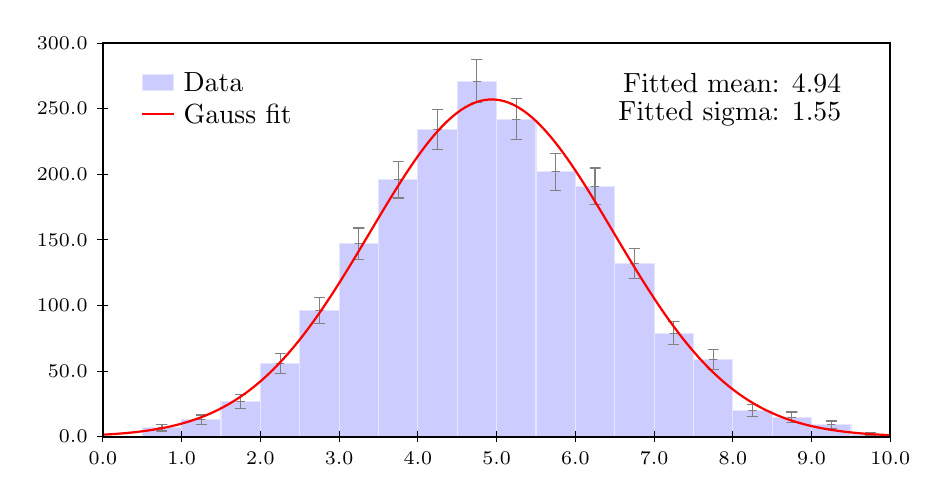
\begin{tikzpicture}
\node[left] at (9.5,4.5) {Fitted mean:  4.94};
\node[left] at (9.5,4.1) {Fitted sigma:  1.55};
\begin{scope}[]
\pgfpathmoveto{ \pgfpointxy {0.0} {0.0}}
\pgfpathlineto{ \pgfpointxy {10.0} {0.0}}
\pgfpathlineto{ \pgfpointxy {10.0} {5.0}}
\pgfpathlineto{ \pgfpointxy {0.0} {5.0}}
\pgfpathclose
\pgfusepath{  clip, }
\begin{scope}[shift={(0.0,0.0)}]
\pgfsetxvec{\pgfpoint{1.0cm}{0cm}}
\pgfsetyvec{\pgfpoint{0cm}{0.016666668cm}}
\begin{scope}[shift={(0.0,0.0)}]
\begin{scope}[draw=blue!10,fill=blue!20]
\pgfpathmoveto{ \pgfpointxy {10.0} {0.0}}
\pgfpathlineto{ \pgfpointxy {10.0} {2.0}}
\pgfpathlineto{ \pgfpointxy {9.5} {2.0}}
\pgfpathlineto{ \pgfpointxy {9.5} {9.0}}
\pgfpathlineto{ \pgfpointxy {9.0} {9.0}}
\pgfpathlineto{ \pgfpointxy {9.0} {15.0}}
\pgfpathlineto{ \pgfpointxy {8.5} {15.0}}
\pgfpathlineto{ \pgfpointxy {8.5} {20.0}}
\pgfpathlineto{ \pgfpointxy {8.0} {20.0}}
\pgfpathlineto{ \pgfpointxy {8.0} {59.0}}
\pgfpathlineto{ \pgfpointxy {7.5} {59.0}}
\pgfpathlineto{ \pgfpointxy {7.5} {79.0}}
\pgfpathlineto{ \pgfpointxy {7.0} {79.0}}
\pgfpathlineto{ \pgfpointxy {7.0} {132.0}}
\pgfpathlineto{ \pgfpointxy {6.5} {132.0}}
\pgfpathlineto{ \pgfpointxy {6.5} {191.0}}
\pgfpathlineto{ \pgfpointxy {6.0} {191.0}}
\pgfpathlineto{ \pgfpointxy {6.0} {202.0}}
\pgfpathlineto{ \pgfpointxy {5.5} {202.0}}
\pgfpathlineto{ \pgfpointxy {5.5} {242.0}}
\pgfpathlineto{ \pgfpointxy {5.0} {242.0}}
\pgfpathlineto{ \pgfpointxy {5.0} {271.0}}
\pgfpathlineto{ \pgfpointxy {4.5} {271.0}}
\pgfpathlineto{ \pgfpointxy {4.5} {234.0}}
\pgfpathlineto{ \pgfpointxy {4.0} {234.0}}
\pgfpathlineto{ \pgfpointxy {4.0} {196.0}}
\pgfpathlineto{ \pgfpointxy {3.5} {196.0}}
\pgfpathlineto{ \pgfpointxy {3.5} {147.0}}
\pgfpathlineto{ \pgfpointxy {3.0} {147.0}}
\pgfpathlineto{ \pgfpointxy {3.0} {96.0}}
\pgfpathlineto{ \pgfpointxy {2.5} {96.0}}
\pgfpathlineto{ \pgfpointxy {2.5} {56.0}}
\pgfpathlineto{ \pgfpointxy {2.0} {56.0}}
\pgfpathlineto{ \pgfpointxy {2.0} {27.0}}
\pgfpathlineto{ \pgfpointxy {1.5} {27.0}}
\pgfpathlineto{ \pgfpointxy {1.5} {13.0}}
\pgfpathlineto{ \pgfpointxy {1.0} {13.0}}
\pgfpathlineto{ \pgfpointxy {1.0} {7.0}}
\pgfpathlineto{ \pgfpointxy {0.5} {7.0}}
\pgfpathlineto{ \pgfpointxy {0.5} {0.0}}
\pgfpathlineto{ \pgfpointxy {0.0} {0.0}}
\pgfpathlineto{ \pgfpointxy {0.0} {0.0}}
\pgfusepath{ stroke, fill, }
\end{scope}
\begin{scope}[draw=blue!10,fill=blue!20]
\pgfpathmoveto{ \pgfpointxy {10.0} {0.0}}
\pgfpathlineto{ \pgfpointxy {10.0} {0.0}}
\pgfusepath{ stroke, }
\end{scope}
\begin{scope}[draw=blue!10,fill=blue!20]
\pgfpathmoveto{ \pgfpointxy {10.0} {2.0}}
\pgfpathlineto{ \pgfpointxy {10.0} {0.0}}
\pgfusepath{ stroke, }
\end{scope}
\begin{scope}[draw=blue!10,fill=blue!20]
\pgfpathmoveto{ \pgfpointxy {9.5} {2.0}}
\pgfpathlineto{ \pgfpointxy {9.5} {0.0}}
\pgfusepath{ stroke, }
\end{scope}
\begin{scope}[draw=blue!10,fill=blue!20]
\pgfpathmoveto{ \pgfpointxy {9.5} {9.0}}
\pgfpathlineto{ \pgfpointxy {9.5} {0.0}}
\pgfusepath{ stroke, }
\end{scope}
\begin{scope}[draw=blue!10,fill=blue!20]
\pgfpathmoveto{ \pgfpointxy {9.0} {9.0}}
\pgfpathlineto{ \pgfpointxy {9.0} {0.0}}
\pgfusepath{ stroke, }
\end{scope}
\begin{scope}[draw=blue!10,fill=blue!20]
\pgfpathmoveto{ \pgfpointxy {9.0} {15.0}}
\pgfpathlineto{ \pgfpointxy {9.0} {0.0}}
\pgfusepath{ stroke, }
\end{scope}
\begin{scope}[draw=blue!10,fill=blue!20]
\pgfpathmoveto{ \pgfpointxy {8.5} {15.0}}
\pgfpathlineto{ \pgfpointxy {8.5} {0.0}}
\pgfusepath{ stroke, }
\end{scope}
\begin{scope}[draw=blue!10,fill=blue!20]
\pgfpathmoveto{ \pgfpointxy {8.5} {20.0}}
\pgfpathlineto{ \pgfpointxy {8.5} {0.0}}
\pgfusepath{ stroke, }
\end{scope}
\begin{scope}[draw=blue!10,fill=blue!20]
\pgfpathmoveto{ \pgfpointxy {8.0} {20.0}}
\pgfpathlineto{ \pgfpointxy {8.0} {0.0}}
\pgfusepath{ stroke, }
\end{scope}
\begin{scope}[draw=blue!10,fill=blue!20]
\pgfpathmoveto{ \pgfpointxy {8.0} {59.0}}
\pgfpathlineto{ \pgfpointxy {8.0} {0.0}}
\pgfusepath{ stroke, }
\end{scope}
\begin{scope}[draw=blue!10,fill=blue!20]
\pgfpathmoveto{ \pgfpointxy {7.5} {59.0}}
\pgfpathlineto{ \pgfpointxy {7.5} {0.0}}
\pgfusepath{ stroke, }
\end{scope}
\begin{scope}[draw=blue!10,fill=blue!20]
\pgfpathmoveto{ \pgfpointxy {7.5} {79.0}}
\pgfpathlineto{ \pgfpointxy {7.5} {0.0}}
\pgfusepath{ stroke, }
\end{scope}
\begin{scope}[draw=blue!10,fill=blue!20]
\pgfpathmoveto{ \pgfpointxy {7.0} {79.0}}
\pgfpathlineto{ \pgfpointxy {7.0} {0.0}}
\pgfusepath{ stroke, }
\end{scope}
\begin{scope}[draw=blue!10,fill=blue!20]
\pgfpathmoveto{ \pgfpointxy {7.0} {132.0}}
\pgfpathlineto{ \pgfpointxy {7.0} {0.0}}
\pgfusepath{ stroke, }
\end{scope}
\begin{scope}[draw=blue!10,fill=blue!20]
\pgfpathmoveto{ \pgfpointxy {6.5} {132.0}}
\pgfpathlineto{ \pgfpointxy {6.5} {0.0}}
\pgfusepath{ stroke, }
\end{scope}
\begin{scope}[draw=blue!10,fill=blue!20]
\pgfpathmoveto{ \pgfpointxy {6.5} {191.0}}
\pgfpathlineto{ \pgfpointxy {6.5} {0.0}}
\pgfusepath{ stroke, }
\end{scope}
\begin{scope}[draw=blue!10,fill=blue!20]
\pgfpathmoveto{ \pgfpointxy {6.0} {191.0}}
\pgfpathlineto{ \pgfpointxy {6.0} {0.0}}
\pgfusepath{ stroke, }
\end{scope}
\begin{scope}[draw=blue!10,fill=blue!20]
\pgfpathmoveto{ \pgfpointxy {6.0} {202.0}}
\pgfpathlineto{ \pgfpointxy {6.0} {0.0}}
\pgfusepath{ stroke, }
\end{scope}
\begin{scope}[draw=blue!10,fill=blue!20]
\pgfpathmoveto{ \pgfpointxy {5.5} {202.0}}
\pgfpathlineto{ \pgfpointxy {5.5} {0.0}}
\pgfusepath{ stroke, }
\end{scope}
\begin{scope}[draw=blue!10,fill=blue!20]
\pgfpathmoveto{ \pgfpointxy {5.5} {242.0}}
\pgfpathlineto{ \pgfpointxy {5.5} {0.0}}
\pgfusepath{ stroke, }
\end{scope}
\begin{scope}[draw=blue!10,fill=blue!20]
\pgfpathmoveto{ \pgfpointxy {5.0} {242.0}}
\pgfpathlineto{ \pgfpointxy {5.0} {0.0}}
\pgfusepath{ stroke, }
\end{scope}
\begin{scope}[draw=blue!10,fill=blue!20]
\pgfpathmoveto{ \pgfpointxy {5.0} {271.0}}
\pgfpathlineto{ \pgfpointxy {5.0} {0.0}}
\pgfusepath{ stroke, }
\end{scope}
\begin{scope}[draw=blue!10,fill=blue!20]
\pgfpathmoveto{ \pgfpointxy {4.5} {271.0}}
\pgfpathlineto{ \pgfpointxy {4.5} {0.0}}
\pgfusepath{ stroke, }
\end{scope}
\begin{scope}[draw=blue!10,fill=blue!20]
\pgfpathmoveto{ \pgfpointxy {4.5} {234.0}}
\pgfpathlineto{ \pgfpointxy {4.5} {0.0}}
\pgfusepath{ stroke, }
\end{scope}
\begin{scope}[draw=blue!10,fill=blue!20]
\pgfpathmoveto{ \pgfpointxy {4.0} {234.0}}
\pgfpathlineto{ \pgfpointxy {4.0} {0.0}}
\pgfusepath{ stroke, }
\end{scope}
\begin{scope}[draw=blue!10,fill=blue!20]
\pgfpathmoveto{ \pgfpointxy {4.0} {196.0}}
\pgfpathlineto{ \pgfpointxy {4.0} {0.0}}
\pgfusepath{ stroke, }
\end{scope}
\begin{scope}[draw=blue!10,fill=blue!20]
\pgfpathmoveto{ \pgfpointxy {3.5} {196.0}}
\pgfpathlineto{ \pgfpointxy {3.5} {0.0}}
\pgfusepath{ stroke, }
\end{scope}
\begin{scope}[draw=blue!10,fill=blue!20]
\pgfpathmoveto{ \pgfpointxy {3.5} {147.0}}
\pgfpathlineto{ \pgfpointxy {3.5} {0.0}}
\pgfusepath{ stroke, }
\end{scope}
\begin{scope}[draw=blue!10,fill=blue!20]
\pgfpathmoveto{ \pgfpointxy {3.0} {147.0}}
\pgfpathlineto{ \pgfpointxy {3.0} {0.0}}
\pgfusepath{ stroke, }
\end{scope}
\begin{scope}[draw=blue!10,fill=blue!20]
\pgfpathmoveto{ \pgfpointxy {3.0} {96.0}}
\pgfpathlineto{ \pgfpointxy {3.0} {0.0}}
\pgfusepath{ stroke, }
\end{scope}
\begin{scope}[draw=blue!10,fill=blue!20]
\pgfpathmoveto{ \pgfpointxy {2.5} {96.0}}
\pgfpathlineto{ \pgfpointxy {2.5} {0.0}}
\pgfusepath{ stroke, }
\end{scope}
\begin{scope}[draw=blue!10,fill=blue!20]
\pgfpathmoveto{ \pgfpointxy {2.5} {56.0}}
\pgfpathlineto{ \pgfpointxy {2.5} {0.0}}
\pgfusepath{ stroke, }
\end{scope}
\begin{scope}[draw=blue!10,fill=blue!20]
\pgfpathmoveto{ \pgfpointxy {2.0} {56.0}}
\pgfpathlineto{ \pgfpointxy {2.0} {0.0}}
\pgfusepath{ stroke, }
\end{scope}
\begin{scope}[draw=blue!10,fill=blue!20]
\pgfpathmoveto{ \pgfpointxy {2.0} {27.0}}
\pgfpathlineto{ \pgfpointxy {2.0} {0.0}}
\pgfusepath{ stroke, }
\end{scope}
\begin{scope}[draw=blue!10,fill=blue!20]
\pgfpathmoveto{ \pgfpointxy {1.5} {27.0}}
\pgfpathlineto{ \pgfpointxy {1.5} {0.0}}
\pgfusepath{ stroke, }
\end{scope}
\begin{scope}[draw=blue!10,fill=blue!20]
\pgfpathmoveto{ \pgfpointxy {1.5} {13.0}}
\pgfpathlineto{ \pgfpointxy {1.5} {0.0}}
\pgfusepath{ stroke, }
\end{scope}
\begin{scope}[draw=blue!10,fill=blue!20]
\pgfpathmoveto{ \pgfpointxy {1.0} {13.0}}
\pgfpathlineto{ \pgfpointxy {1.0} {0.0}}
\pgfusepath{ stroke, }
\end{scope}
\begin{scope}[draw=blue!10,fill=blue!20]
\pgfpathmoveto{ \pgfpointxy {1.0} {7.0}}
\pgfpathlineto{ \pgfpointxy {1.0} {0.0}}
\pgfusepath{ stroke, }
\end{scope}
\begin{scope}[draw=blue!10,fill=blue!20]
\pgfpathmoveto{ \pgfpointxy {0.5} {7.0}}
\pgfpathlineto{ \pgfpointxy {0.5} {0.0}}
\pgfusepath{ stroke, }
\end{scope}
\begin{scope}[draw=blue!10,fill=blue!20]
\pgfpathmoveto{ \pgfpointxy {0.5} {0.0}}
\pgfpathlineto{ \pgfpointxy {0.5} {0.0}}
\pgfusepath{ stroke, }
\end{scope}
\begin{scope}[draw=blue!10,fill=blue!20]
\pgfpathmoveto{ \pgfpointxy {0.0} {0.0}}
\pgfpathlineto{ \pgfpointxy {0.0} {0.0}}
\pgfusepath{ stroke, }
\end{scope}
\begin{scope}[draw=blue!10,fill=blue!20]
\pgfpathmoveto{ \pgfpointxy {0.0} {0.0}}
\pgfpathlineto{ \pgfpointxy {0.0} {0.0}}
\pgfusepath{ stroke, }
\end{scope}
\begin{scope}[draw=gray,fill=gray]
\pgfpointadd{\pgfpointxy {0.25} {0.0}} {\pgfpoint{-2pt}{0}}\pgfpathmoveto{ NIL }
\pgfpointadd{\pgfpointxy {0.25} {0.0}} {\pgfpoint{2pt}{0}}\pgfpathlineto{ NIL }
\pgfpointadd{\pgfpointxy {0.25} {0.0}} {\pgfpoint{0pt}{0}}\pgfpathlineto{ NIL }
\pgfpointadd{\pgfpointxy {0.25} {0.0}} {\pgfpoint{0pt}{0}}\pgfpathlineto{ NIL }
\pgfpointadd{\pgfpointxy {0.25} {0.0}} {\pgfpoint{-2pt}{0}}\pgfpathlineto{ NIL }
\pgfpointadd{\pgfpointxy {0.25} {0.0}} {\pgfpoint{2pt}{0}}\pgfpathlineto{ NIL }
\pgfusepath{ stroke, }
\node at (0.25,0.0) [rectangle,inner sep=0.0pt,minimum width =3.0pt,minimum height=0.0pt,draw=gray,fill=gray] {}; 
\end{scope}
\begin{scope}[draw=gray,fill=gray]
\pgfpointadd{\pgfpointxy {0.75} {9.645751}} {\pgfpoint{-2pt}{0}}\pgfpathmoveto{ NIL }
\pgfpointadd{\pgfpointxy {0.75} {9.645751}} {\pgfpoint{2pt}{0}}\pgfpathlineto{ NIL }
\pgfpointadd{\pgfpointxy {0.75} {9.645751}} {\pgfpoint{0pt}{0}}\pgfpathlineto{ NIL }
\pgfpointadd{\pgfpointxy {0.75} {4.354249}} {\pgfpoint{0pt}{0}}\pgfpathlineto{ NIL }
\pgfpointadd{\pgfpointxy {0.75} {4.354249}} {\pgfpoint{-2pt}{0}}\pgfpathlineto{ NIL }
\pgfpointadd{\pgfpointxy {0.75} {4.354249}} {\pgfpoint{2pt}{0}}\pgfpathlineto{ NIL }
\pgfusepath{ stroke, }
\node at (0.75,7.0) [rectangle,inner sep=0.0pt,minimum width =3.0pt,minimum height=0.0pt,draw=gray,fill=gray] {}; 
\end{scope}
\begin{scope}[draw=gray,fill=gray]
\pgfpointadd{\pgfpointxy {1.25} {16.60555}} {\pgfpoint{-2pt}{0}}\pgfpathmoveto{ NIL }
\pgfpointadd{\pgfpointxy {1.25} {16.60555}} {\pgfpoint{2pt}{0}}\pgfpathlineto{ NIL }
\pgfpointadd{\pgfpointxy {1.25} {16.60555}} {\pgfpoint{0pt}{0}}\pgfpathlineto{ NIL }
\pgfpointadd{\pgfpointxy {1.25} {9.394449}} {\pgfpoint{0pt}{0}}\pgfpathlineto{ NIL }
\pgfpointadd{\pgfpointxy {1.25} {9.394449}} {\pgfpoint{-2pt}{0}}\pgfpathlineto{ NIL }
\pgfpointadd{\pgfpointxy {1.25} {9.394449}} {\pgfpoint{2pt}{0}}\pgfpathlineto{ NIL }
\pgfusepath{ stroke, }
\node at (1.25,13.0) [rectangle,inner sep=0.0pt,minimum width =3.0pt,minimum height=0.0pt,draw=gray,fill=gray] {}; 
\end{scope}
\begin{scope}[draw=gray,fill=gray]
\pgfpointadd{\pgfpointxy {1.75} {32.19615}} {\pgfpoint{-2pt}{0}}\pgfpathmoveto{ NIL }
\pgfpointadd{\pgfpointxy {1.75} {32.19615}} {\pgfpoint{2pt}{0}}\pgfpathlineto{ NIL }
\pgfpointadd{\pgfpointxy {1.75} {32.19615}} {\pgfpoint{0pt}{0}}\pgfpathlineto{ NIL }
\pgfpointadd{\pgfpointxy {1.75} {21.803848}} {\pgfpoint{0pt}{0}}\pgfpathlineto{ NIL }
\pgfpointadd{\pgfpointxy {1.75} {21.803848}} {\pgfpoint{-2pt}{0}}\pgfpathlineto{ NIL }
\pgfpointadd{\pgfpointxy {1.75} {21.803848}} {\pgfpoint{2pt}{0}}\pgfpathlineto{ NIL }
\pgfusepath{ stroke, }
\node at (1.75,27.0) [rectangle,inner sep=0.0pt,minimum width =3.0pt,minimum height=0.0pt,draw=gray,fill=gray] {}; 
\end{scope}
\begin{scope}[draw=gray,fill=gray]
\pgfpointadd{\pgfpointxy {2.25} {63.483315}} {\pgfpoint{-2pt}{0}}\pgfpathmoveto{ NIL }
\pgfpointadd{\pgfpointxy {2.25} {63.483315}} {\pgfpoint{2pt}{0}}\pgfpathlineto{ NIL }
\pgfpointadd{\pgfpointxy {2.25} {63.483315}} {\pgfpoint{0pt}{0}}\pgfpathlineto{ NIL }
\pgfpointadd{\pgfpointxy {2.25} {48.516685}} {\pgfpoint{0pt}{0}}\pgfpathlineto{ NIL }
\pgfpointadd{\pgfpointxy {2.25} {48.516685}} {\pgfpoint{-2pt}{0}}\pgfpathlineto{ NIL }
\pgfpointadd{\pgfpointxy {2.25} {48.516685}} {\pgfpoint{2pt}{0}}\pgfpathlineto{ NIL }
\pgfusepath{ stroke, }
\node at (2.25,56.0) [rectangle,inner sep=0.0pt,minimum width =3.0pt,minimum height=0.0pt,draw=gray,fill=gray] {}; 
\end{scope}
\begin{scope}[draw=gray,fill=gray]
\pgfpointadd{\pgfpointxy {2.75} {105.79796}} {\pgfpoint{-2pt}{0}}\pgfpathmoveto{ NIL }
\pgfpointadd{\pgfpointxy {2.75} {105.79796}} {\pgfpoint{2pt}{0}}\pgfpathlineto{ NIL }
\pgfpointadd{\pgfpointxy {2.75} {105.79796}} {\pgfpoint{0pt}{0}}\pgfpathlineto{ NIL }
\pgfpointadd{\pgfpointxy {2.75} {86.20204}} {\pgfpoint{0pt}{0}}\pgfpathlineto{ NIL }
\pgfpointadd{\pgfpointxy {2.75} {86.20204}} {\pgfpoint{-2pt}{0}}\pgfpathlineto{ NIL }
\pgfpointadd{\pgfpointxy {2.75} {86.20204}} {\pgfpoint{2pt}{0}}\pgfpathlineto{ NIL }
\pgfusepath{ stroke, }
\node at (2.75,96.0) [rectangle,inner sep=0.0pt,minimum width =3.0pt,minimum height=0.0pt,draw=gray,fill=gray] {}; 
\end{scope}
\begin{scope}[draw=gray,fill=gray]
\pgfpointadd{\pgfpointxy {3.25} {159.12436}} {\pgfpoint{-2pt}{0}}\pgfpathmoveto{ NIL }
\pgfpointadd{\pgfpointxy {3.25} {159.12436}} {\pgfpoint{2pt}{0}}\pgfpathlineto{ NIL }
\pgfpointadd{\pgfpointxy {3.25} {159.12436}} {\pgfpoint{0pt}{0}}\pgfpathlineto{ NIL }
\pgfpointadd{\pgfpointxy {3.25} {134.87564}} {\pgfpoint{0pt}{0}}\pgfpathlineto{ NIL }
\pgfpointadd{\pgfpointxy {3.25} {134.87564}} {\pgfpoint{-2pt}{0}}\pgfpathlineto{ NIL }
\pgfpointadd{\pgfpointxy {3.25} {134.87564}} {\pgfpoint{2pt}{0}}\pgfpathlineto{ NIL }
\pgfusepath{ stroke, }
\node at (3.25,147.0) [rectangle,inner sep=0.0pt,minimum width =3.0pt,minimum height=0.0pt,draw=gray,fill=gray] {}; 
\end{scope}
\begin{scope}[draw=gray,fill=gray]
\pgfpointadd{\pgfpointxy {3.75} {210.0}} {\pgfpoint{-2pt}{0}}\pgfpathmoveto{ NIL }
\pgfpointadd{\pgfpointxy {3.75} {210.0}} {\pgfpoint{2pt}{0}}\pgfpathlineto{ NIL }
\pgfpointadd{\pgfpointxy {3.75} {210.0}} {\pgfpoint{0pt}{0}}\pgfpathlineto{ NIL }
\pgfpointadd{\pgfpointxy {3.75} {182.0}} {\pgfpoint{0pt}{0}}\pgfpathlineto{ NIL }
\pgfpointadd{\pgfpointxy {3.75} {182.0}} {\pgfpoint{-2pt}{0}}\pgfpathlineto{ NIL }
\pgfpointadd{\pgfpointxy {3.75} {182.0}} {\pgfpoint{2pt}{0}}\pgfpathlineto{ NIL }
\pgfusepath{ stroke, }
\node at (3.75,196.0) [rectangle,inner sep=0.0pt,minimum width =3.0pt,minimum height=0.0pt,draw=gray,fill=gray] {}; 
\end{scope}
\begin{scope}[draw=gray,fill=gray]
\pgfpointadd{\pgfpointxy {4.25} {249.29706}} {\pgfpoint{-2pt}{0}}\pgfpathmoveto{ NIL }
\pgfpointadd{\pgfpointxy {4.25} {249.29706}} {\pgfpoint{2pt}{0}}\pgfpathlineto{ NIL }
\pgfpointadd{\pgfpointxy {4.25} {249.29706}} {\pgfpoint{0pt}{0}}\pgfpathlineto{ NIL }
\pgfpointadd{\pgfpointxy {4.25} {218.70294}} {\pgfpoint{0pt}{0}}\pgfpathlineto{ NIL }
\pgfpointadd{\pgfpointxy {4.25} {218.70294}} {\pgfpoint{-2pt}{0}}\pgfpathlineto{ NIL }
\pgfpointadd{\pgfpointxy {4.25} {218.70294}} {\pgfpoint{2pt}{0}}\pgfpathlineto{ NIL }
\pgfusepath{ stroke, }
\node at (4.25,234.0) [rectangle,inner sep=0.0pt,minimum width =3.0pt,minimum height=0.0pt,draw=gray,fill=gray] {}; 
\end{scope}
\begin{scope}[draw=gray,fill=gray]
\pgfpointadd{\pgfpointxy {4.75} {287.46207}} {\pgfpoint{-2pt}{0}}\pgfpathmoveto{ NIL }
\pgfpointadd{\pgfpointxy {4.75} {287.46207}} {\pgfpoint{2pt}{0}}\pgfpathlineto{ NIL }
\pgfpointadd{\pgfpointxy {4.75} {287.46207}} {\pgfpoint{0pt}{0}}\pgfpathlineto{ NIL }
\pgfpointadd{\pgfpointxy {4.75} {254.53792}} {\pgfpoint{0pt}{0}}\pgfpathlineto{ NIL }
\pgfpointadd{\pgfpointxy {4.75} {254.53792}} {\pgfpoint{-2pt}{0}}\pgfpathlineto{ NIL }
\pgfpointadd{\pgfpointxy {4.75} {254.53792}} {\pgfpoint{2pt}{0}}\pgfpathlineto{ NIL }
\pgfusepath{ stroke, }
\node at (4.75,271.0) [rectangle,inner sep=0.0pt,minimum width =3.0pt,minimum height=0.0pt,draw=gray,fill=gray] {}; 
\end{scope}
\begin{scope}[draw=gray,fill=gray]
\pgfpointadd{\pgfpointxy {5.25} {257.55634}} {\pgfpoint{-2pt}{0}}\pgfpathmoveto{ NIL }
\pgfpointadd{\pgfpointxy {5.25} {257.55634}} {\pgfpoint{2pt}{0}}\pgfpathlineto{ NIL }
\pgfpointadd{\pgfpointxy {5.25} {257.55634}} {\pgfpoint{0pt}{0}}\pgfpathlineto{ NIL }
\pgfpointadd{\pgfpointxy {5.25} {226.44365}} {\pgfpoint{0pt}{0}}\pgfpathlineto{ NIL }
\pgfpointadd{\pgfpointxy {5.25} {226.44365}} {\pgfpoint{-2pt}{0}}\pgfpathlineto{ NIL }
\pgfpointadd{\pgfpointxy {5.25} {226.44365}} {\pgfpoint{2pt}{0}}\pgfpathlineto{ NIL }
\pgfusepath{ stroke, }
\node at (5.25,242.0) [rectangle,inner sep=0.0pt,minimum width =3.0pt,minimum height=0.0pt,draw=gray,fill=gray] {}; 
\end{scope}
\begin{scope}[draw=gray,fill=gray]
\pgfpointadd{\pgfpointxy {5.75} {216.21268}} {\pgfpoint{-2pt}{0}}\pgfpathmoveto{ NIL }
\pgfpointadd{\pgfpointxy {5.75} {216.21268}} {\pgfpoint{2pt}{0}}\pgfpathlineto{ NIL }
\pgfpointadd{\pgfpointxy {5.75} {216.21268}} {\pgfpoint{0pt}{0}}\pgfpathlineto{ NIL }
\pgfpointadd{\pgfpointxy {5.75} {187.78732}} {\pgfpoint{0pt}{0}}\pgfpathlineto{ NIL }
\pgfpointadd{\pgfpointxy {5.75} {187.78732}} {\pgfpoint{-2pt}{0}}\pgfpathlineto{ NIL }
\pgfpointadd{\pgfpointxy {5.75} {187.78732}} {\pgfpoint{2pt}{0}}\pgfpathlineto{ NIL }
\pgfusepath{ stroke, }
\node at (5.75,202.0) [rectangle,inner sep=0.0pt,minimum width =3.0pt,minimum height=0.0pt,draw=gray,fill=gray] {}; 
\end{scope}
\begin{scope}[draw=gray,fill=gray]
\pgfpointadd{\pgfpointxy {6.25} {204.82028}} {\pgfpoint{-2pt}{0}}\pgfpathmoveto{ NIL }
\pgfpointadd{\pgfpointxy {6.25} {204.82028}} {\pgfpoint{2pt}{0}}\pgfpathlineto{ NIL }
\pgfpointadd{\pgfpointxy {6.25} {204.82028}} {\pgfpoint{0pt}{0}}\pgfpathlineto{ NIL }
\pgfpointadd{\pgfpointxy {6.25} {177.17972}} {\pgfpoint{0pt}{0}}\pgfpathlineto{ NIL }
\pgfpointadd{\pgfpointxy {6.25} {177.17972}} {\pgfpoint{-2pt}{0}}\pgfpathlineto{ NIL }
\pgfpointadd{\pgfpointxy {6.25} {177.17972}} {\pgfpoint{2pt}{0}}\pgfpathlineto{ NIL }
\pgfusepath{ stroke, }
\node at (6.25,191.0) [rectangle,inner sep=0.0pt,minimum width =3.0pt,minimum height=0.0pt,draw=gray,fill=gray] {}; 
\end{scope}
\begin{scope}[draw=gray,fill=gray]
\pgfpointadd{\pgfpointxy {6.75} {143.48912}} {\pgfpoint{-2pt}{0}}\pgfpathmoveto{ NIL }
\pgfpointadd{\pgfpointxy {6.75} {143.48912}} {\pgfpoint{2pt}{0}}\pgfpathlineto{ NIL }
\pgfpointadd{\pgfpointxy {6.75} {143.48912}} {\pgfpoint{0pt}{0}}\pgfpathlineto{ NIL }
\pgfpointadd{\pgfpointxy {6.75} {120.51087}} {\pgfpoint{0pt}{0}}\pgfpathlineto{ NIL }
\pgfpointadd{\pgfpointxy {6.75} {120.51087}} {\pgfpoint{-2pt}{0}}\pgfpathlineto{ NIL }
\pgfpointadd{\pgfpointxy {6.75} {120.51087}} {\pgfpoint{2pt}{0}}\pgfpathlineto{ NIL }
\pgfusepath{ stroke, }
\node at (6.75,132.0) [rectangle,inner sep=0.0pt,minimum width =3.0pt,minimum height=0.0pt,draw=gray,fill=gray] {}; 
\end{scope}
\begin{scope}[draw=gray,fill=gray]
\pgfpointadd{\pgfpointxy {7.25} {87.88819}} {\pgfpoint{-2pt}{0}}\pgfpathmoveto{ NIL }
\pgfpointadd{\pgfpointxy {7.25} {87.88819}} {\pgfpoint{2pt}{0}}\pgfpathlineto{ NIL }
\pgfpointadd{\pgfpointxy {7.25} {87.88819}} {\pgfpoint{0pt}{0}}\pgfpathlineto{ NIL }
\pgfpointadd{\pgfpointxy {7.25} {70.11181}} {\pgfpoint{0pt}{0}}\pgfpathlineto{ NIL }
\pgfpointadd{\pgfpointxy {7.25} {70.11181}} {\pgfpoint{-2pt}{0}}\pgfpathlineto{ NIL }
\pgfpointadd{\pgfpointxy {7.25} {70.11181}} {\pgfpoint{2pt}{0}}\pgfpathlineto{ NIL }
\pgfusepath{ stroke, }
\node at (7.25,79.0) [rectangle,inner sep=0.0pt,minimum width =3.0pt,minimum height=0.0pt,draw=gray,fill=gray] {}; 
\end{scope}
\begin{scope}[draw=gray,fill=gray]
\pgfpointadd{\pgfpointxy {7.75} {66.681145}} {\pgfpoint{-2pt}{0}}\pgfpathmoveto{ NIL }
\pgfpointadd{\pgfpointxy {7.75} {66.681145}} {\pgfpoint{2pt}{0}}\pgfpathlineto{ NIL }
\pgfpointadd{\pgfpointxy {7.75} {66.681145}} {\pgfpoint{0pt}{0}}\pgfpathlineto{ NIL }
\pgfpointadd{\pgfpointxy {7.75} {51.318855}} {\pgfpoint{0pt}{0}}\pgfpathlineto{ NIL }
\pgfpointadd{\pgfpointxy {7.75} {51.318855}} {\pgfpoint{-2pt}{0}}\pgfpathlineto{ NIL }
\pgfpointadd{\pgfpointxy {7.75} {51.318855}} {\pgfpoint{2pt}{0}}\pgfpathlineto{ NIL }
\pgfusepath{ stroke, }
\node at (7.75,59.0) [rectangle,inner sep=0.0pt,minimum width =3.0pt,minimum height=0.0pt,draw=gray,fill=gray] {}; 
\end{scope}
\begin{scope}[draw=gray,fill=gray]
\pgfpointadd{\pgfpointxy {8.25} {24.472136}} {\pgfpoint{-2pt}{0}}\pgfpathmoveto{ NIL }
\pgfpointadd{\pgfpointxy {8.25} {24.472136}} {\pgfpoint{2pt}{0}}\pgfpathlineto{ NIL }
\pgfpointadd{\pgfpointxy {8.25} {24.472136}} {\pgfpoint{0pt}{0}}\pgfpathlineto{ NIL }
\pgfpointadd{\pgfpointxy {8.25} {15.527864}} {\pgfpoint{0pt}{0}}\pgfpathlineto{ NIL }
\pgfpointadd{\pgfpointxy {8.25} {15.527864}} {\pgfpoint{-2pt}{0}}\pgfpathlineto{ NIL }
\pgfpointadd{\pgfpointxy {8.25} {15.527864}} {\pgfpoint{2pt}{0}}\pgfpathlineto{ NIL }
\pgfusepath{ stroke, }
\node at (8.25,20.0) [rectangle,inner sep=0.0pt,minimum width =3.0pt,minimum height=0.0pt,draw=gray,fill=gray] {}; 
\end{scope}
\begin{scope}[draw=gray,fill=gray]
\pgfpointadd{\pgfpointxy {8.75} {18.872984}} {\pgfpoint{-2pt}{0}}\pgfpathmoveto{ NIL }
\pgfpointadd{\pgfpointxy {8.75} {18.872984}} {\pgfpoint{2pt}{0}}\pgfpathlineto{ NIL }
\pgfpointadd{\pgfpointxy {8.75} {18.872984}} {\pgfpoint{0pt}{0}}\pgfpathlineto{ NIL }
\pgfpointadd{\pgfpointxy {8.75} {11.127016}} {\pgfpoint{0pt}{0}}\pgfpathlineto{ NIL }
\pgfpointadd{\pgfpointxy {8.75} {11.127016}} {\pgfpoint{-2pt}{0}}\pgfpathlineto{ NIL }
\pgfpointadd{\pgfpointxy {8.75} {11.127016}} {\pgfpoint{2pt}{0}}\pgfpathlineto{ NIL }
\pgfusepath{ stroke, }
\node at (8.75,15.0) [rectangle,inner sep=0.0pt,minimum width =3.0pt,minimum height=0.0pt,draw=gray,fill=gray] {}; 
\end{scope}
\begin{scope}[draw=gray,fill=gray]
\pgfpointadd{\pgfpointxy {9.25} {12.0}} {\pgfpoint{-2pt}{0}}\pgfpathmoveto{ NIL }
\pgfpointadd{\pgfpointxy {9.25} {12.0}} {\pgfpoint{2pt}{0}}\pgfpathlineto{ NIL }
\pgfpointadd{\pgfpointxy {9.25} {12.0}} {\pgfpoint{0pt}{0}}\pgfpathlineto{ NIL }
\pgfpointadd{\pgfpointxy {9.25} {6.0}} {\pgfpoint{0pt}{0}}\pgfpathlineto{ NIL }
\pgfpointadd{\pgfpointxy {9.25} {6.0}} {\pgfpoint{-2pt}{0}}\pgfpathlineto{ NIL }
\pgfpointadd{\pgfpointxy {9.25} {6.0}} {\pgfpoint{2pt}{0}}\pgfpathlineto{ NIL }
\pgfusepath{ stroke, }
\node at (9.25,9.0) [rectangle,inner sep=0.0pt,minimum width =3.0pt,minimum height=0.0pt,draw=gray,fill=gray] {}; 
\end{scope}
\begin{scope}[draw=gray,fill=gray]
\pgfpointadd{\pgfpointxy {9.75} {3.4142137}} {\pgfpoint{-2pt}{0}}\pgfpathmoveto{ NIL }
\pgfpointadd{\pgfpointxy {9.75} {3.4142137}} {\pgfpoint{2pt}{0}}\pgfpathlineto{ NIL }
\pgfpointadd{\pgfpointxy {9.75} {3.4142137}} {\pgfpoint{0pt}{0}}\pgfpathlineto{ NIL }
\pgfpointadd{\pgfpointxy {9.75} {0.58578646}} {\pgfpoint{0pt}{0}}\pgfpathlineto{ NIL }
\pgfpointadd{\pgfpointxy {9.75} {0.58578646}} {\pgfpoint{-2pt}{0}}\pgfpathlineto{ NIL }
\pgfpointadd{\pgfpointxy {9.75} {0.58578646}} {\pgfpoint{2pt}{0}}\pgfpathlineto{ NIL }
\pgfusepath{ stroke, }
\node at (9.75,2.0) [rectangle,inner sep=0.0pt,minimum width =3.0pt,minimum height=0.0pt,draw=gray,fill=gray] {}; 
\end{scope}
\begin{scope}[thick,red]
\pgfpathmoveto{ \pgfpointxy {0.0} {1.558576020676866}}
\pgfpathlineto{ \pgfpointxy {0.05} {1.7274503227501066}}
\pgfpathlineto{ \pgfpointxy {0.1} {1.9126188963667363}}
\pgfpathlineto{ \pgfpointxy {0.15} {2.1154200480403227}}
\pgfpathlineto{ \pgfpointxy {0.2} {2.3372764756403903}}
\pgfpathlineto{ \pgfpointxy {0.25} {2.5796979496539985}}
\pgfpathlineto{ \pgfpointxy {0.3} {2.8442837980858506}}
\pgfpathlineto{ \pgfpointxy {0.35} {3.132725158018863}}
\pgfpathlineto{ \pgfpointxy {0.4} {3.4468069547981615}}
\pgfpathlineto{ \pgfpointxy {0.45} {3.7884095678724714}}
\pgfpathlineto{ \pgfpointxy {0.5} {4.159510140559981}}
\pgfpathlineto{ \pgfpointxy {0.55} {4.562183489434911}}
\pgfpathlineto{ \pgfpointxy {0.6} {4.99860256769178}}
\pgfpathlineto{ \pgfpointxy {0.65} {5.471038435772837}}
\pgfpathlineto{ \pgfpointxy {0.7} {5.981859691776892}}
\pgfpathlineto{ \pgfpointxy {0.75} {6.533531313743065}}
\pgfpathlineto{ \pgfpointxy {0.8} {7.128612865856165}}
\pgfpathlineto{ \pgfpointxy {0.85} {7.769756020989981}}
\pgfpathlineto{ \pgfpointxy {0.9} {8.459701352824242}}
\pgfpathlineto{ \pgfpointxy {0.95} {9.201274352075282}}
\pgfpathlineto{ \pgfpointxy {1.0} {9.997380623200701}}
\pgfpathlineto{ \pgfpointxy {1.05} {10.85100022030292}}
\pgfpathlineto{ \pgfpointxy {1.1} {11.765181083891807}}
\pgfpathlineto{ \pgfpointxy {1.15} {12.74303154369313}}
\pgfpathlineto{ \pgfpointxy {1.2} {13.78771185682457}}
\pgfpathlineto{ \pgfpointxy {1.25} {14.902424755416321}}
\pgfpathlineto{ \pgfpointxy {1.3} {16.090404983135112}}
\pgfpathlineto{ \pgfpointxy {1.35} {17.354907806077094}}
\pgfpathlineto{ \pgfpointxy {1.4} {18.699196490121263}}
\pgfpathlineto{ \pgfpointxy {1.45} {20.12652874406518}}
\pgfpathlineto{ \pgfpointxy {1.5} {21.640142135675536}}
\pgfpathlineto{ \pgfpointxy {1.55} {23.24323849615082}}
\pgfpathlineto{ \pgfpointxy {1.6} {24.938967337367576}}
\pgfpathlineto{ \pgfpointxy {1.65} {26.7304083156247}}
\pgfpathlineto{ \pgfpointxy {1.7} {28.62055278535065}}
\pgfpathlineto{ \pgfpointxy {1.75} {30.612284496334055}}
\pgfpathlineto{ \pgfpointxy {1.8} {32.70835949840771}}
\pgfpathlineto{ \pgfpointxy {1.85} {34.91138532807266}}
\pgfpathlineto{ \pgfpointxy {1.9} {37.22379956221061}}
\pgfpathlineto{ \pgfpointxy {1.95} {39.64784783469681}}
\pgfpathlineto{ \pgfpointxy {2.0} {42.185561422291414}}
\pgfpathlineto{ \pgfpointxy {2.05} {44.838734516545586}}
\pgfpathlineto{ \pgfpointxy {2.1} {47.60890130849298}}
\pgfpathlineto{ \pgfpointxy {2.15} {50.4973130224912}}
\pgfpathlineto{ \pgfpointxy {2.2} {53.504915044608836}}
\pgfpathlineto{ \pgfpointxy {2.25} {56.632324299297366}}
\pgfpathlineto{ \pgfpointxy {2.3} {59.87980703562242}}
\pgfpathlineto{ \pgfpointxy {2.35} {63.24725719093013}}
\pgfpathlineto{ \pgfpointxy {2.4} {66.73417550537421}}
\pgfpathlineto{ \pgfpointxy {2.45} {70.33964956511109}}
\pgfpathlineto{ \pgfpointxy {2.5} {74.06233495507152}}
\pgfpathlineto{ \pgfpointxy {2.55} {77.90043770394169}}
\pgfpathlineto{ \pgfpointxy {2.6} {81.85169820423305}}
\pgfpathlineto{ \pgfpointxy {2.65} {85.91337678901114}}
\pgfpathlineto{ \pgfpointxy {2.7} {90.08224114391795}}
\pgfpathlineto{ \pgfpointxy {2.75} {94.35455572849908}}
\pgfpathlineto{ \pgfpointxy {2.8} {98.72607337450253}}
\pgfpathlineto{ \pgfpointxy {2.85} {103.19202922071392}}
\pgfpathlineto{ \pgfpointxy {2.9} {107.74713713403635}}
\pgfpathlineto{ \pgfpointxy {2.95} {112.38558875491714}}
\pgfpathlineto{ \pgfpointxy {3.0} {117.10105529189481}}
\pgfpathlineto{ \pgfpointxy {3.05} {121.88669217504761}}
\pgfpathlineto{ \pgfpointxy {3.1} {126.73514666152779}}
\pgfpathlineto{ \pgfpointxy {3.15} {131.63856846826192}}
\pgfpathlineto{ \pgfpointxy {3.2} {136.58862348739274}}
\pgfpathlineto{ \pgfpointxy {3.25} {141.57651061926111}}
\pgfpathlineto{ \pgfpointxy {3.3} {146.59298173583076}}
\pgfpathlineto{ \pgfpointxy {3.35} {151.62836476460035}}
\pgfpathlineto{ \pgfpointxy {3.4} {156.67258985942038}}
\pgfpathlineto{ \pgfpointxy {3.45} {161.7152186004281}}
\pgfpathlineto{ \pgfpointxy {3.5} {166.74547614073975}}
\pgfpathlineto{ \pgfpointxy {3.55} {171.75228619282998}}
\pgfpathlineto{ \pgfpointxy {3.6} {176.72430872290073}}
\pgfpathlineto{ \pgfpointxy {3.65} {181.6499801972455}}
\pgfpathlineto{ \pgfpointxy {3.7} {186.5175562008881}}
\pgfpathlineto{ \pgfpointxy {3.75} {191.31515622585772}}
\pgfpathlineto{ \pgfpointxy {3.8} {196.03081040460765}}
\pgfpathlineto{ \pgfpointxy {3.85} {200.65250794351792}}
\pgfpathlineto{ \pgfpointxy {3.9} {205.1682469923884}}
\pgfpathlineto{ \pgfpointxy {3.95} {209.56608566853743}}
\pgfpathlineto{ \pgfpointxy {4.0} {213.83419393878864}}
\pgfpathlineto{ \pgfpointxy {4.05} {217.9609060494452}}
\pgfpathlineto{ \pgfpointxy {4.1} {221.93477318349133}}
\pgfpathlineto{ \pgfpointxy {4.15} {225.74461601588078}}
\pgfpathlineto{ \pgfpointxy {4.2} {229.3795768320013}}
\pgfpathlineto{ \pgfpointxy {4.25} {232.82917087135112}}
\pgfpathlineto{ \pgfpointxy {4.3} {236.08333655820527}}
\pgfpathlineto{ \pgfpointxy {4.35} {239.13248428364233}}
\pgfpathlineto{ \pgfpointxy {4.4} {241.9675434087641}}
\pgfpathlineto{ \pgfpointxy {4.45} {244.58000716726772}}
\pgfpathlineto{ \pgfpointxy {4.5} {246.9619751566839}}
\pgfpathlineto{ \pgfpointxy {4.55} {249.1061931215066}}
\pgfpathlineto{ \pgfpointxy {4.6} {251.00608974801486}}
\pgfpathlineto{ \pgfpointxy {4.65} {252.6558102096966}}
\pgfpathlineto{ \pgfpointxy {4.7} {254.05024622367264}}
\pgfpathlineto{ \pgfpointxy {4.75} {255.18506240220933}}
\pgfpathlineto{ \pgfpointxy {4.8} {256.0567187090879}}
\pgfpathlineto{ \pgfpointxy {4.85} {256.6624888580471}}
\pgfpathlineto{ \pgfpointxy {4.9} {257.0004745194776}}
\pgfpathlineto{ \pgfpointxy {4.95} {257.06961523176074}}
\pgfpathlineto{ \pgfpointxy {5.0} {256.86969394483054}}
\pgfpathlineto{ \pgfpointxy {5.05} {256.401338155402}}
\pgfpathlineto{ \pgfpointxy {5.1} {255.66601662555647}}
\pgfpathlineto{ \pgfpointxy {5.15} {254.66603170869865}}
\pgfpathlineto{ \pgfpointxy {5.2} {253.40450733900056}}
\pgfpathlineto{ \pgfpointxy {5.25} {251.88537277201746}}
\pgfpathlineto{ \pgfpointxy {5.3} {250.11334219491098}}
\pgfpathlineto{ \pgfpointxy {5.35} {248.0938903543545}}
\pgfpathlineto{ \pgfpointxy {5.4} {245.83322437845325}}
\pgfpathlineto{ \pgfpointxy {5.45} {243.33825199563105}}
\pgfpathlineto{ \pgfpointxy {5.5} {240.61654637817384}}
\pgfpathlineto{ \pgfpointxy {5.55} {237.6763078607661}}
\pgfpathlineto{ \pgfpointxy {5.6} {234.52632280470687}}
\pgfpathlineto{ \pgfpointxy {5.65} {231.17591989638905}}
\pgfpathlineto{ \pgfpointxy {5.7} {227.63492418391843}}
\pgfpathlineto{ \pgfpointxy {5.75} {223.9136091683304}}
\pgfpathlineto{ \pgfpointxy {5.8} {220.02264727565102}}
\pgfpathlineto{ \pgfpointxy {5.85} {215.9730590429822}}
\pgfpathlineto{ \pgfpointxy {5.9} {211.77616135586024}}
\pgfpathlineto{ \pgfpointxy {5.95} {207.44351507533685}}
\pgfpathlineto{ \pgfpointxy {6.0} {202.9868723916073}}
\pgfpathlineto{ \pgfpointxy {6.05} {198.41812423662532}}
\pgfpathlineto{ \pgfpointxy {6.1} {193.74924808108875}}
\pgfpathlineto{ \pgfpointxy {6.15} {188.99225643157735}}
\pgfpathlineto{ \pgfpointxy {6.2} {184.1591463316151}}
\pgfpathlineto{ \pgfpointxy {6.25} {179.26185015617526}}
\pgfpathlineto{ \pgfpointxy {6.3} {174.31218797284095}}
\pgfpathlineto{ \pgfpointxy {6.35} {169.32182172466466}}
\pgfpathlineto{ \pgfpointxy {6.4} {164.30221146996436}}
\pgfpathlineto{ \pgfpointxy {6.45} {159.26457389307188}}
\pgfpathlineto{ \pgfpointxy {6.5} {154.21984327764548}}
\pgfpathlineto{ \pgfpointxy {6.55} {149.17863511082155}}
\pgfpathlineto{ \pgfpointxy {6.6} {144.151212462442}}
\pgfpathlineto{ \pgfpointxy {6.65} {139.14745525910845}}
\pgfpathlineto{ \pgfpointxy {6.7} {134.17683254811797}}
\pgfpathlineto{ \pgfpointxy {6.75} {129.24837782166048}}
\pgfpathlineto{ \pgfpointxy {6.8} {124.37066744724133}}
\pgfpathlineto{ \pgfpointxy {6.85} {119.55180222633848}}
\pgfpathlineto{ \pgfpointxy {6.9} {114.79939208002902}}
\pgfpathlineto{ \pgfpointxy {6.95} {110.12054383790831}}
\pgfpathlineto{ \pgfpointxy {7.0} {105.52185208525077}}
\pgfpathlineto{ \pgfpointxy {7.05} {101.00939300318913}}
\pgfpathlineto{ \pgfpointxy {7.1} {96.58872111784704}}
\pgfpathlineto{ \pgfpointxy {7.15} {92.26486885697777}}
\pgfpathlineto{ \pgfpointxy {7.2} {88.04234879683506}}
\pgfpathlineto{ \pgfpointxy {7.25} {83.92515846780941}}
\pgfpathlineto{ \pgfpointxy {7.3} {79.91678757487001}}
\pgfpathlineto{ \pgfpointxy {7.35} {76.02022747809175}}
\pgfpathlineto{ \pgfpointxy {7.4} {72.23798276954341}}
\pgfpathlineto{ \pgfpointxy {7.45} {68.57208477556978}}
\pgfpathlineto{ \pgfpointxy {7.5} {65.02410680799369}}
\pgfpathlineto{ \pgfpointxy {7.55} {61.59518098397015}}
\pgfpathlineto{ \pgfpointxy {7.6} {58.28601643208637}}
\pgfpathlineto{ \pgfpointxy {7.65} {55.09691870175808}}
\pgfpathlineto{ \pgfpointxy {7.7} {52.02781019395011}}
\pgfpathlineto{ \pgfpointxy {7.75} {49.07825143365233}}
\pgfpathlineto{ \pgfpointxy {7.8} {46.24746300828272}}
\pgfpathlineto{ \pgfpointxy {7.85} {43.53434800114982}}
\pgfpathlineto{ \pgfpointxy {7.9} {40.937514755184765}}
\pgfpathlineto{ \pgfpointxy {7.95} {38.45529980922224}}
\pgfpathlineto{ \pgfpointxy {8.0} {36.085790857054135}}
\pgfpathlineto{ \pgfpointxy {8.05} {33.82684958817274}}
\pgfpathlineto{ \pgfpointxy {8.1} {31.6761342784406}}
\pgfpathlineto{ \pgfpointxy {8.15} {29.631122008746036}}
\pgfpathlineto{ \pgfpointxy {8.2} {27.689130399912187}}
\pgfpathlineto{ \pgfpointxy {8.25} {25.847338762597456}}
\pgfpathlineto{ \pgfpointxy {8.3} {24.10280857155552}}
\pgfpathlineto{ \pgfpointxy {8.35} {22.452503184295036}}
\pgfpathlineto{ \pgfpointxy {8.4} {20.89330673480372}}
\pgfpathlineto{ \pgfpointxy {8.45} {19.42204214347753}}
\pgfpathlineto{ \pgfpointxy {8.5} {18.03548819463977}}
\pgfpathlineto{ \pgfpointxy {8.55} {16.73039564297438}}
\pgfpathlineto{ \pgfpointxy {8.6} {15.503502319754952}}
\pgfpathlineto{ \pgfpointxy {8.65} {14.351547218873485}}
\pgfpathlineto{ \pgfpointxy {8.7} {13.271283551305883}}
\pgfpathlineto{ \pgfpointxy {8.75} {12.259490764748348}}
\pgfpathlineto{ \pgfpointxy {8.8} {11.312985532693581}}
\pgfpathlineto{ \pgfpointxy {8.85} {10.428631724151984}}
\pgfpathlineto{ \pgfpointxy {8.9} {9.603349371550834}}
\pgfpathlineto{ \pgfpointxy {8.95} {8.834122660047734}}
\pgfpathlineto{ \pgfpointxy {9.0} {8.118006966570197}}
\pgfpathlineto{ \pgfpointxy {9.05} {7.452134981347872}}
\pgfpathlineto{ \pgfpointxy {9.1} {6.8337219485391705}}
\pgfpathlineto{ \pgfpointxy {9.15} {6.260070065792449}}
\pgfpathlineto{ \pgfpointxy {9.2} {5.72857208523604}}
\pgfpathlineto{ \pgfpointxy {9.25} {5.236714160487787}}
\pgfpathlineto{ \pgfpointxy {9.3} {4.78207798584115}}
\pgfpathlineto{ \pgfpointxy {9.35} {4.362342274848571}}
\pgfpathlineto{ \pgfpointxy {9.4} {3.975283626119874}}
\pgfpathlineto{ \pgfpointxy {9.45} {3.6187768243158493}}
\pgfpathlineto{ \pgfpointxy {9.5} {3.290794624081893}}
\pgfpathlineto{ \pgfpointxy {9.55} {2.9894070640710915}}
\pgfpathlineto{ \pgfpointxy {9.6} {2.712780357285991}}
\pgfpathlineto{ \pgfpointxy {9.65} {2.459175402762056}}
\pgfpathlineto{ \pgfpointxy {9.7} {2.2269459621598866}}
\pgfpathlineto{ \pgfpointxy {9.75} {2.014536543162128}}
\pgfpathlineto{ \pgfpointxy {9.8} {1.8204800297218426}}
\pgfpathlineto{ \pgfpointxy {9.85} {1.6433950972124476}}
\pgfpathlineto{ \pgfpointxy {9.9} {1.4819834484189018}}
\pgfpathlineto{ \pgfpointxy {9.95} {1.335026904114285}}
\pgfpathlineto{ \pgfpointxy {10.0} {1.2013843797131074}}
\pgfusepath{ stroke, }
\end{scope}
\end{scope}
\pgfsetxvec{\pgfpoint{1cm}{0cm}}
\pgfsetyvec{\pgfpoint{0cm}{1cm}}
\end{scope}
\end{scope}
\begin{scope}[shift={(0.0,0.0)}]
\pgfsetxvec{\pgfpoint{1.0cm}{0cm}}
\pgfsetyvec{\pgfpoint{0cm}{0.016666668cm}}
\begin{scope}[shift={(0.0,0.0)}]
\begin{scope}[thick,black,fill=white]
\pgfpathmoveto{ \pgfpointxy {0.0} {0.0}}
\pgfpathlineto{ \pgfpointxy {10.0} {0.0}}
\pgfpathlineto{ \pgfpointxy {10.0} {300.0}}
\pgfpathlineto{ \pgfpointxy {0.0} {300.0}}
\pgfpathclose
\pgfusepath{ stroke, }
\end{scope}
\begin{scope}[yshift=0cm]
\draw[] [shift={(0.0,0.0)}] (0,2pt) -- (0,-2pt) node[below]{ \scriptsize{\num[round-mode=places,round-precision=1]{0.0}}};
\draw[] [shift={(1.0,0.0)}] (0,2pt) -- (0,-2pt) node[below]{ \scriptsize{\num[round-mode=places,round-precision=1]{1.0}}};
\draw[] [shift={(2.0,0.0)}] (0,2pt) -- (0,-2pt) node[below]{ \scriptsize{\num[round-mode=places,round-precision=1]{2.0}}};
\draw[] [shift={(3.0,0.0)}] (0,2pt) -- (0,-2pt) node[below]{ \scriptsize{\num[round-mode=places,round-precision=1]{3.0}}};
\draw[] [shift={(4.0,0.0)}] (0,2pt) -- (0,-2pt) node[below]{ \scriptsize{\num[round-mode=places,round-precision=1]{4.0}}};
\draw[] [shift={(5.0,0.0)}] (0,2pt) -- (0,-2pt) node[below]{ \scriptsize{\num[round-mode=places,round-precision=1]{5.0}}};
\draw[] [shift={(6.0,0.0)}] (0,2pt) -- (0,-2pt) node[below]{ \scriptsize{\num[round-mode=places,round-precision=1]{6.0}}};
\draw[] [shift={(7.0,0.0)}] (0,2pt) -- (0,-2pt) node[below]{ \scriptsize{\num[round-mode=places,round-precision=1]{7.0}}};
\draw[] [shift={(8.0,0.0)}] (0,2pt) -- (0,-2pt) node[below]{ \scriptsize{\num[round-mode=places,round-precision=1]{8.0}}};
\draw[] [shift={(9.0,0.0)}] (0,2pt) -- (0,-2pt) node[below]{ \scriptsize{\num[round-mode=places,round-precision=1]{9.0}}};
\draw[] [shift={(10.0,0.0)}] (0,2pt) -- (0,-2pt) node[below]{ \scriptsize{\num[round-mode=places,round-precision=1]{10.0}}};
\end{scope}
\begin{scope}[xshift=0cm]
\draw[] [shift={(0.0,0.0)}] (2pt,0) -- (-2pt,0) node[left]{ \scriptsize{\num[round-mode=places,round-precision=1]{0.0}}};
\draw[] [shift={(0.0,50.0)}] (2pt,0) -- (-2pt,0) node[left]{ \scriptsize{\num[round-mode=places,round-precision=1]{50.0}}};
\draw[] [shift={(0.0,100.0)}] (2pt,0) -- (-2pt,0) node[left]{ \scriptsize{\num[round-mode=places,round-precision=1]{100.0}}};
\draw[] [shift={(0.0,150.0)}] (2pt,0) -- (-2pt,0) node[left]{ \scriptsize{\num[round-mode=places,round-precision=1]{150.0}}};
\draw[] [shift={(0.0,200.0)}] (2pt,0) -- (-2pt,0) node[left]{ \scriptsize{\num[round-mode=places,round-precision=1]{200.0}}};
\draw[] [shift={(0.0,250.0)}] (2pt,0) -- (-2pt,0) node[left]{ \scriptsize{\num[round-mode=places,round-precision=1]{250.0}}};
\draw[] [shift={(0.0,300.0)}] (2pt,0) -- (-2pt,0) node[left]{ \scriptsize{\num[round-mode=places,round-precision=1]{300.0}}};
\end{scope}
\end{scope}
\pgfsetxvec{\pgfpoint{1cm}{0cm}}
\pgfsetyvec{\pgfpoint{0cm}{1cm}}
\end{scope}
\draw[draw=blue!10,fill=blue!20] (0.5,4.4) rectangle (0.9,4.6);
\node[right,] at (0.9,4.5) {Data};
\draw[thick,red] (0.5,4.1) -- (0.9,4.1);
\node[right,] at (0.9,4.1) {Gauss fit};
\end{tikzpicture}
\end{document}

  \caption{The Gaussian function fitted to histogram made from 2000 gaussian random numbers}
\end{figure}

\begin{figure}[H]
  \centering
  %%% AUTO GENERATED CODE
\documentclass{standalone}
\ifx\HCode\UnDef\else\def\pgfsysdriver{pgfsys-tex4ht.def}\fi
\usepackage[usenames,dvipsnames,svgnames,table]{xcolor}
\usepackage{tikz}
\usepackage{color}
\usepackage{siunitx}
\usetikzlibrary{arrows,shapes}
\begin{document}
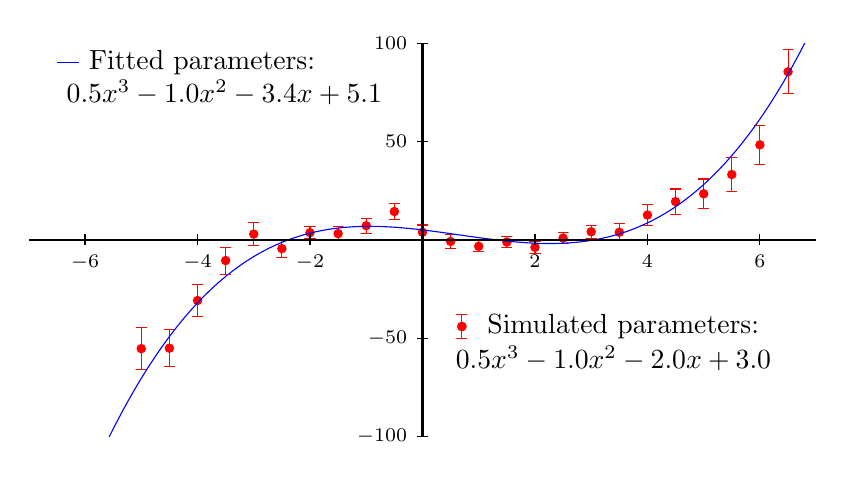
\begin{tikzpicture}
\begin{scope}[]
\pgfpathmoveto{ \pgfpointadd{\pgfpointxy {0.0} {0.0}} {\pgfpoint{0cm}{0cm}} }
\pgfpathlineto{ \pgfpointadd{\pgfpointxy {0.0} {0.0}} {\pgfpoint{10cm}{0cm}} }
\pgfpathlineto{ \pgfpointadd{\pgfpointxy {0.0} {0.0}} {\pgfpoint{10cm}{5cm}} }
\pgfpathlineto{ \pgfpointadd{\pgfpointxy {0.0} {0.0}} {\pgfpoint{0cm}{5cm}} }
\pgfpathclose
\pgfusepath{  clip, }
\begin{scope}[shift={(0.0,0.0)}]
\pgfsetxvec{\pgfpoint{0.71428573cm}{0cm}}
\pgfsetyvec{\pgfpoint{0cm}{0.025cm}}
\begin{scope}[shift={(7.0,100.0)}]
\begin{scope}[draw=red,fill=red]
\pgfpathmoveto{ \pgfpointadd{\pgfpointxy {-10.0} {-571.0535387380919}} {\pgfpoint{-2pt}{0}} }
\pgfpathlineto{ \pgfpointadd{\pgfpointxy {-10.0} {-571.0535387380919}} {\pgfpoint{2pt}{0}} }
\pgfpathlineto{ \pgfpointadd{\pgfpointxy {-10.0} {-571.0535387380919}} {\pgfpoint{0pt}{0}} }
\pgfpathlineto{ \pgfpointadd{\pgfpointxy {-10.0} {-623.095187335949}} {\pgfpoint{0pt}{0}} }
\pgfpathlineto{ \pgfpointadd{\pgfpointxy {-10.0} {-623.095187335949}} {\pgfpoint{-2pt}{0}} }
\pgfpathlineto{ \pgfpointadd{\pgfpointxy {-10.0} {-623.095187335949}} {\pgfpoint{2pt}{0}} }
\pgfusepath{ stroke, }
\node at (-10.0,-597.0743630370205) [draw=red,fill=red,circle,inner sep=0.0pt,minimum width =3.0pt,minimum height=3.0pt] {};
\end{scope}
\begin{scope}[draw=red,fill=red]
\pgfpathmoveto{ \pgfpointadd{\pgfpointxy {-9.5} {-465.4942843469761}} {\pgfpoint{-2pt}{0}} }
\pgfpathlineto{ \pgfpointadd{\pgfpointxy {-9.5} {-465.4942843469761}} {\pgfpoint{2pt}{0}} }
\pgfpathlineto{ \pgfpointadd{\pgfpointxy {-9.5} {-465.4942843469761}} {\pgfpoint{0pt}{0}} }
\pgfpathlineto{ \pgfpointadd{\pgfpointxy {-9.5} {-514.0784743698979}} {\pgfpoint{0pt}{0}} }
\pgfpathlineto{ \pgfpointadd{\pgfpointxy {-9.5} {-514.0784743698979}} {\pgfpoint{-2pt}{0}} }
\pgfpathlineto{ \pgfpointadd{\pgfpointxy {-9.5} {-514.0784743698979}} {\pgfpoint{2pt}{0}} }
\pgfusepath{ stroke, }
\node at (-9.5,-489.786379358437) [draw=red,fill=red,circle,inner sep=0.0pt,minimum width =3.0pt,minimum height=3.0pt] {};
\end{scope}
\begin{scope}[draw=red,fill=red]
\pgfpathmoveto{ \pgfpointadd{\pgfpointxy {-9.0} {-412.1044371552097}} {\pgfpoint{-2pt}{0}} }
\pgfpathlineto{ \pgfpointadd{\pgfpointxy {-9.0} {-412.1044371552097}} {\pgfpoint{2pt}{0}} }
\pgfpathlineto{ \pgfpointadd{\pgfpointxy {-9.0} {-412.1044371552097}} {\pgfpoint{0pt}{0}} }
\pgfpathlineto{ \pgfpointadd{\pgfpointxy {-9.0} {-457.3112327112828}} {\pgfpoint{0pt}{0}} }
\pgfpathlineto{ \pgfpointadd{\pgfpointxy {-9.0} {-457.3112327112828}} {\pgfpoint{-2pt}{0}} }
\pgfpathlineto{ \pgfpointadd{\pgfpointxy {-9.0} {-457.3112327112828}} {\pgfpoint{2pt}{0}} }
\pgfusepath{ stroke, }
\node at (-9.0,-434.70783493324626) [draw=red,fill=red,circle,inner sep=0.0pt,minimum width =3.0pt,minimum height=3.0pt] {};
\end{scope}
\begin{scope}[draw=red,fill=red]
\pgfpathmoveto{ \pgfpointadd{\pgfpointxy {-8.5} {-357.183759168102}} {\pgfpoint{-2pt}{0}} }
\pgfpathlineto{ \pgfpointadd{\pgfpointxy {-8.5} {-357.183759168102}} {\pgfpoint{2pt}{0}} }
\pgfpathlineto{ \pgfpointadd{\pgfpointxy {-8.5} {-357.183759168102}} {\pgfpoint{0pt}{0}} }
\pgfpathlineto{ \pgfpointadd{\pgfpointxy {-8.5} {-399.0948393426367}} {\pgfpoint{0pt}{0}} }
\pgfpathlineto{ \pgfpointadd{\pgfpointxy {-8.5} {-399.0948393426367}} {\pgfpoint{-2pt}{0}} }
\pgfpathlineto{ \pgfpointadd{\pgfpointxy {-8.5} {-399.0948393426367}} {\pgfpoint{2pt}{0}} }
\pgfusepath{ stroke, }
\node at (-8.5,-378.13929925536934) [draw=red,fill=red,circle,inner sep=0.0pt,minimum width =3.0pt,minimum height=3.0pt] {};
\end{scope}
\begin{scope}[draw=red,fill=red]
\pgfpathmoveto{ \pgfpointadd{\pgfpointxy {-8.0} {-291.87829172373085}} {\pgfpoint{-2pt}{0}} }
\pgfpathlineto{ \pgfpointadd{\pgfpointxy {-8.0} {-291.87829172373085}} {\pgfpoint{2pt}{0}} }
\pgfpathlineto{ \pgfpointadd{\pgfpointxy {-8.0} {-291.87829172373085}} {\pgfpoint{0pt}{0}} }
\pgfpathlineto{ \pgfpointadd{\pgfpointxy {-8.0} {-330.57699486952583}} {\pgfpoint{0pt}{0}} }
\pgfpathlineto{ \pgfpointadd{\pgfpointxy {-8.0} {-330.57699486952583}} {\pgfpoint{-2pt}{0}} }
\pgfpathlineto{ \pgfpointadd{\pgfpointxy {-8.0} {-330.57699486952583}} {\pgfpoint{2pt}{0}} }
\pgfusepath{ stroke, }
\node at (-8.0,-311.22764329662834) [draw=red,fill=red,circle,inner sep=0.0pt,minimum width =3.0pt,minimum height=3.0pt] {};
\end{scope}
\begin{scope}[draw=red,fill=red]
\pgfpathmoveto{ \pgfpointadd{\pgfpointxy {-7.5} {-238.3149428018001}} {\pgfpoint{-2pt}{0}} }
\pgfpathlineto{ \pgfpointadd{\pgfpointxy {-7.5} {-238.3149428018001}} {\pgfpoint{2pt}{0}} }
\pgfpathlineto{ \pgfpointadd{\pgfpointxy {-7.5} {-238.3149428018001}} {\pgfpoint{0pt}{0}} }
\pgfpathlineto{ \pgfpointadd{\pgfpointxy {-7.5} {-273.88629057157385}} {\pgfpoint{0pt}{0}} }
\pgfpathlineto{ \pgfpointadd{\pgfpointxy {-7.5} {-273.88629057157385}} {\pgfpoint{-2pt}{0}} }
\pgfpathlineto{ \pgfpointadd{\pgfpointxy {-7.5} {-273.88629057157385}} {\pgfpoint{2pt}{0}} }
\pgfusepath{ stroke, }
\node at (-7.5,-256.100616686687) [draw=red,fill=red,circle,inner sep=0.0pt,minimum width =3.0pt,minimum height=3.0pt] {};
\end{scope}
\begin{scope}[draw=red,fill=red]
\pgfpathmoveto{ \pgfpointadd{\pgfpointxy {-7.0} {-202.29808062975653}} {\pgfpoint{-2pt}{0}} }
\pgfpathlineto{ \pgfpointadd{\pgfpointxy {-7.0} {-202.29808062975653}} {\pgfpoint{2pt}{0}} }
\pgfpathlineto{ \pgfpointadd{\pgfpointxy {-7.0} {-202.29808062975653}} {\pgfpoint{0pt}{0}} }
\pgfpathlineto{ \pgfpointadd{\pgfpointxy {-7.0} {-234.82876586513075}} {\pgfpoint{0pt}{0}} }
\pgfpathlineto{ \pgfpointadd{\pgfpointxy {-7.0} {-234.82876586513075}} {\pgfpoint{-2pt}{0}} }
\pgfpathlineto{ \pgfpointadd{\pgfpointxy {-7.0} {-234.82876586513075}} {\pgfpoint{2pt}{0}} }
\pgfusepath{ stroke, }
\node at (-7.0,-218.56342324744364) [draw=red,fill=red,circle,inner sep=0.0pt,minimum width =3.0pt,minimum height=3.0pt] {};
\end{scope}
\begin{scope}[draw=red,fill=red]
\pgfpathmoveto{ \pgfpointadd{\pgfpointxy {-6.5} {-145.7322270733457}} {\pgfpoint{-2pt}{0}} }
\pgfpathlineto{ \pgfpointadd{\pgfpointxy {-6.5} {-145.7322270733457}} {\pgfpoint{2pt}{0}} }
\pgfpathlineto{ \pgfpointadd{\pgfpointxy {-6.5} {-145.7322270733457}} {\pgfpoint{0pt}{0}} }
\pgfpathlineto{ \pgfpointadd{\pgfpointxy {-6.5} {-175.31053819820306}} {\pgfpoint{0pt}{0}} }
\pgfpathlineto{ \pgfpointadd{\pgfpointxy {-6.5} {-175.31053819820306}} {\pgfpoint{-2pt}{0}} }
\pgfpathlineto{ \pgfpointadd{\pgfpointxy {-6.5} {-175.31053819820306}} {\pgfpoint{2pt}{0}} }
\pgfusepath{ stroke, }
\node at (-6.5,-160.5213826357744) [draw=red,fill=red,circle,inner sep=0.0pt,minimum width =3.0pt,minimum height=3.0pt] {};
\end{scope}
\begin{scope}[draw=red,fill=red]
\pgfpathmoveto{ \pgfpointadd{\pgfpointxy {-6.0} {-109.22115465709189}} {\pgfpoint{-2pt}{0}} }
\pgfpathlineto{ \pgfpointadd{\pgfpointxy {-6.0} {-109.22115465709189}} {\pgfpoint{2pt}{0}} }
\pgfpathlineto{ \pgfpointadd{\pgfpointxy {-6.0} {-109.22115465709189}} {\pgfpoint{0pt}{0}} }
\pgfpathlineto{ \pgfpointadd{\pgfpointxy {-6.0} {-135.93678804029298}} {\pgfpoint{0pt}{0}} }
\pgfpathlineto{ \pgfpointadd{\pgfpointxy {-6.0} {-135.93678804029298}} {\pgfpoint{-2pt}{0}} }
\pgfpathlineto{ \pgfpointadd{\pgfpointxy {-6.0} {-135.93678804029298}} {\pgfpoint{2pt}{0}} }
\pgfusepath{ stroke, }
\node at (-6.0,-122.57897134869243) [draw=red,fill=red,circle,inner sep=0.0pt,minimum width =3.0pt,minimum height=3.0pt] {};
\end{scope}
\begin{scope}[draw=red,fill=red]
\pgfpathmoveto{ \pgfpointadd{\pgfpointxy {-5.5} {-109.25232418508995}} {\pgfpoint{-2pt}{0}} }
\pgfpathlineto{ \pgfpointadd{\pgfpointxy {-5.5} {-109.25232418508995}} {\pgfpoint{2pt}{0}} }
\pgfpathlineto{ \pgfpointadd{\pgfpointxy {-5.5} {-109.25232418508995}} {\pgfpoint{0pt}{0}} }
\pgfpathlineto{ \pgfpointadd{\pgfpointxy {-5.5} {-133.19599486026908}} {\pgfpoint{0pt}{0}} }
\pgfpathlineto{ \pgfpointadd{\pgfpointxy {-5.5} {-133.19599486026908}} {\pgfpoint{-2pt}{0}} }
\pgfpathlineto{ \pgfpointadd{\pgfpointxy {-5.5} {-133.19599486026908}} {\pgfpoint{2pt}{0}} }
\pgfusepath{ stroke, }
\node at (-5.5,-121.22415952267951) [draw=red,fill=red,circle,inner sep=0.0pt,minimum width =3.0pt,minimum height=3.0pt] {};
\end{scope}
\begin{scope}[draw=red,fill=red]
\pgfpathmoveto{ \pgfpointadd{\pgfpointxy {-5.0} {-44.62018863682962}} {\pgfpoint{-2pt}{0}} }
\pgfpathlineto{ \pgfpointadd{\pgfpointxy {-5.0} {-44.62018863682962}} {\pgfpoint{2pt}{0}} }
\pgfpathlineto{ \pgfpointadd{\pgfpointxy {-5.0} {-44.62018863682962}} {\pgfpoint{0pt}{0}} }
\pgfpathlineto{ \pgfpointadd{\pgfpointxy {-5.0} {-65.88286513846168}} {\pgfpoint{0pt}{0}} }
\pgfpathlineto{ \pgfpointadd{\pgfpointxy {-5.0} {-65.88286513846168}} {\pgfpoint{-2pt}{0}} }
\pgfpathlineto{ \pgfpointadd{\pgfpointxy {-5.0} {-65.88286513846168}} {\pgfpoint{2pt}{0}} }
\pgfusepath{ stroke, }
\node at (-5.0,-55.25152688764565) [draw=red,fill=red,circle,inner sep=0.0pt,minimum width =3.0pt,minimum height=3.0pt] {};
\end{scope}
\begin{scope}[draw=red,fill=red]
\pgfpathmoveto{ \pgfpointadd{\pgfpointxy {-4.5} {-45.66786522760035}} {\pgfpoint{-2pt}{0}} }
\pgfpathlineto{ \pgfpointadd{\pgfpointxy {-4.5} {-45.66786522760035}} {\pgfpoint{2pt}{0}} }
\pgfpathlineto{ \pgfpointadd{\pgfpointxy {-4.5} {-45.66786522760035}} {\pgfpoint{0pt}{0}} }
\pgfpathlineto{ \pgfpointadd{\pgfpointxy {-4.5} {-64.33926597872156}} {\pgfpoint{0pt}{0}} }
\pgfpathlineto{ \pgfpointadd{\pgfpointxy {-4.5} {-64.33926597872156}} {\pgfpoint{-2pt}{0}} }
\pgfpathlineto{ \pgfpointadd{\pgfpointxy {-4.5} {-64.33926597872156}} {\pgfpoint{2pt}{0}} }
\pgfusepath{ stroke, }
\node at (-4.5,-55.00356560316096) [draw=red,fill=red,circle,inner sep=0.0pt,minimum width =3.0pt,minimum height=3.0pt] {};
\end{scope}
\begin{scope}[draw=red,fill=red]
\pgfpathmoveto{ \pgfpointadd{\pgfpointxy {-4.0} {-22.71518997590085}} {\pgfpoint{-2pt}{0}} }
\pgfpathlineto{ \pgfpointadd{\pgfpointxy {-4.0} {-22.71518997590085}} {\pgfpoint{2pt}{0}} }
\pgfpathlineto{ \pgfpointadd{\pgfpointxy {-4.0} {-22.71518997590085}} {\pgfpoint{0pt}{0}} }
\pgfpathlineto{ \pgfpointadd{\pgfpointxy {-4.0} {-38.880715036497286}} {\pgfpoint{0pt}{0}} }
\pgfpathlineto{ \pgfpointadd{\pgfpointxy {-4.0} {-38.880715036497286}} {\pgfpoint{-2pt}{0}} }
\pgfpathlineto{ \pgfpointadd{\pgfpointxy {-4.0} {-38.880715036497286}} {\pgfpoint{2pt}{0}} }
\pgfusepath{ stroke, }
\node at (-4.0,-30.797952506199067) [draw=red,fill=red,circle,inner sep=0.0pt,minimum width =3.0pt,minimum height=3.0pt] {};
\end{scope}
\begin{scope}[draw=red,fill=red]
\pgfpathmoveto{ \pgfpointadd{\pgfpointxy {-3.5} {-3.623367622026165}} {\pgfpoint{-2pt}{0}} }
\pgfpathlineto{ \pgfpointadd{\pgfpointxy {-3.5} {-3.623367622026165}} {\pgfpoint{2pt}{0}} }
\pgfpathlineto{ \pgfpointadd{\pgfpointxy {-3.5} {-3.623367622026165}} {\pgfpoint{0pt}{0}} }
\pgfpathlineto{ \pgfpointadd{\pgfpointxy {-3.5} {-17.357328788992056}} {\pgfpoint{0pt}{0}} }
\pgfpathlineto{ \pgfpointadd{\pgfpointxy {-3.5} {-17.357328788992056}} {\pgfpoint{-2pt}{0}} }
\pgfpathlineto{ \pgfpointadd{\pgfpointxy {-3.5} {-17.357328788992056}} {\pgfpoint{2pt}{0}} }
\pgfusepath{ stroke, }
\node at (-3.5,-10.490348205509111) [draw=red,fill=red,circle,inner sep=0.0pt,minimum width =3.0pt,minimum height=3.0pt] {};
\end{scope}
\begin{scope}[draw=red,fill=red]
\pgfpathmoveto{ \pgfpointadd{\pgfpointxy {-3.0} {8.659705441078653}} {\pgfpoint{-2pt}{0}} }
\pgfpathlineto{ \pgfpointadd{\pgfpointxy {-3.0} {8.659705441078653}} {\pgfpoint{2pt}{0}} }
\pgfpathlineto{ \pgfpointadd{\pgfpointxy {-3.0} {8.659705441078653}} {\pgfpoint{0pt}{0}} }
\pgfpathlineto{ \pgfpointadd{\pgfpointxy {-3.0} {-2.688763787270882}} {\pgfpoint{0pt}{0}} }
\pgfpathlineto{ \pgfpointadd{\pgfpointxy {-3.0} {-2.688763787270882}} {\pgfpoint{-2pt}{0}} }
\pgfpathlineto{ \pgfpointadd{\pgfpointxy {-3.0} {-2.688763787270882}} {\pgfpoint{2pt}{0}} }
\pgfusepath{ stroke, }
\node at (-3.0,2.985470826903885) [draw=red,fill=red,circle,inner sep=0.0pt,minimum width =3.0pt,minimum height=3.0pt] {};
\end{scope}
\begin{scope}[draw=red,fill=red]
\pgfpathmoveto{ \pgfpointadd{\pgfpointxy {-2.5} {0.03452070884278502}} {\pgfpoint{-2pt}{0}} }
\pgfpathlineto{ \pgfpointadd{\pgfpointxy {-2.5} {0.03452070884278502}} {\pgfpoint{2pt}{0}} }
\pgfpathlineto{ \pgfpointadd{\pgfpointxy {-2.5} {0.03452070884278502}} {\pgfpoint{0pt}{0}} }
\pgfpathlineto{ \pgfpointadd{\pgfpointxy {-2.5} {-8.889908192055266}} {\pgfpoint{0pt}{0}} }
\pgfpathlineto{ \pgfpointadd{\pgfpointxy {-2.5} {-8.889908192055266}} {\pgfpoint{-2pt}{0}} }
\pgfpathlineto{ \pgfpointadd{\pgfpointxy {-2.5} {-8.889908192055266}} {\pgfpoint{2pt}{0}} }
\pgfusepath{ stroke, }
\node at (-2.5,-4.427693741606241) [draw=red,fill=red,circle,inner sep=0.0pt,minimum width =3.0pt,minimum height=3.0pt] {};
\end{scope}
\begin{scope}[draw=red,fill=red]
\pgfpathmoveto{ \pgfpointadd{\pgfpointxy {-2.0} {6.691469768324479}} {\pgfpoint{-2pt}{0}} }
\pgfpathlineto{ \pgfpointadd{\pgfpointxy {-2.0} {6.691469768324479}} {\pgfpoint{2pt}{0}} }
\pgfpathlineto{ \pgfpointadd{\pgfpointxy {-2.0} {6.691469768324479}} {\pgfpoint{0pt}{0}} }
\pgfpathlineto{ \pgfpointadd{\pgfpointxy {-2.0} {0.6914697683244793}} {\pgfpoint{0pt}{0}} }
\pgfpathlineto{ \pgfpointadd{\pgfpointxy {-2.0} {0.6914697683244793}} {\pgfpoint{-2pt}{0}} }
\pgfpathlineto{ \pgfpointadd{\pgfpointxy {-2.0} {0.6914697683244793}} {\pgfpoint{2pt}{0}} }
\pgfusepath{ stroke, }
\node at (-2.0,3.6914697683244793) [draw=red,fill=red,circle,inner sep=0.0pt,minimum width =3.0pt,minimum height=3.0pt] {};
\end{scope}
\begin{scope}[draw=red,fill=red]
\pgfpathmoveto{ \pgfpointadd{\pgfpointxy {-1.5} {6.642849316210677}} {\pgfpoint{-2pt}{0}} }
\pgfpathlineto{ \pgfpointadd{\pgfpointxy {-1.5} {6.642849316210677}} {\pgfpoint{2pt}{0}} }
\pgfpathlineto{ \pgfpointadd{\pgfpointxy {-1.5} {6.642849316210677}} {\pgfpoint{0pt}{0}} }
\pgfpathlineto{ \pgfpointadd{\pgfpointxy {-1.5} {-0.2294320070583371}} {\pgfpoint{0pt}{0}} }
\pgfpathlineto{ \pgfpointadd{\pgfpointxy {-1.5} {-0.2294320070583371}} {\pgfpoint{-2pt}{0}} }
\pgfpathlineto{ \pgfpointadd{\pgfpointxy {-1.5} {-0.2294320070583371}} {\pgfpoint{2pt}{0}} }
\pgfusepath{ stroke, }
\node at (-1.5,3.20670865457617) [draw=red,fill=red,circle,inner sep=0.0pt,minimum width =3.0pt,minimum height=3.0pt] {};
\end{scope}
\begin{scope}[draw=red,fill=red]
\pgfpathmoveto{ \pgfpointadd{\pgfpointxy {-1.0} {11.107898214064939}} {\pgfpoint{-2pt}{0}} }
\pgfpathlineto{ \pgfpointadd{\pgfpointxy {-1.0} {11.107898214064939}} {\pgfpoint{2pt}{0}} }
\pgfpathlineto{ \pgfpointadd{\pgfpointxy {-1.0} {11.107898214064939}} {\pgfpoint{0pt}{0}} }
\pgfpathlineto{ \pgfpointadd{\pgfpointxy {-1.0} {3.3662408272909987}} {\pgfpoint{0pt}{0}} }
\pgfpathlineto{ \pgfpointadd{\pgfpointxy {-1.0} {3.3662408272909987}} {\pgfpoint{-2pt}{0}} }
\pgfpathlineto{ \pgfpointadd{\pgfpointxy {-1.0} {3.3662408272909987}} {\pgfpoint{2pt}{0}} }
\pgfusepath{ stroke, }
\node at (-1.0,7.237069520677969) [draw=red,fill=red,circle,inner sep=0.0pt,minimum width =3.0pt,minimum height=3.0pt] {};
\end{scope}
\begin{scope}[draw=red,fill=red]
\pgfpathmoveto{ \pgfpointadd{\pgfpointxy {-0.5} {18.362804815403905}} {\pgfpoint{-2pt}{0}} }
\pgfpathlineto{ \pgfpointadd{\pgfpointxy {-0.5} {18.362804815403905}} {\pgfpoint{2pt}{0}} }
\pgfpathlineto{ \pgfpointadd{\pgfpointxy {-0.5} {18.362804815403905}} {\pgfpoint{0pt}{0}} }
\pgfpathlineto{ \pgfpointadd{\pgfpointxy {-0.5} {10.522231941469602}} {\pgfpoint{0pt}{0}} }
\pgfpathlineto{ \pgfpointadd{\pgfpointxy {-0.5} {10.522231941469602}} {\pgfpoint{-2pt}{0}} }
\pgfpathlineto{ \pgfpointadd{\pgfpointxy {-0.5} {10.522231941469602}} {\pgfpoint{2pt}{0}} }
\pgfusepath{ stroke, }
\node at (-0.5,14.442518378436754) [draw=red,fill=red,circle,inner sep=0.0pt,minimum width =3.0pt,minimum height=3.0pt] {};
\end{scope}
\begin{scope}[draw=red,fill=red]
\pgfpathmoveto{ \pgfpointadd{\pgfpointxy {0.0} {7.612007955975413}} {\pgfpoint{-2pt}{0}} }
\pgfpathlineto{ \pgfpointadd{\pgfpointxy {0.0} {7.612007955975413}} {\pgfpoint{2pt}{0}} }
\pgfpathlineto{ \pgfpointadd{\pgfpointxy {0.0} {7.612007955975413}} {\pgfpoint{0pt}{0}} }
\pgfpathlineto{ \pgfpointadd{\pgfpointxy {0.0} {0.14790634083765797}} {\pgfpoint{0pt}{0}} }
\pgfpathlineto{ \pgfpointadd{\pgfpointxy {0.0} {0.14790634083765797}} {\pgfpoint{-2pt}{0}} }
\pgfpathlineto{ \pgfpointadd{\pgfpointxy {0.0} {0.14790634083765797}} {\pgfpoint{2pt}{0}} }
\pgfusepath{ stroke, }
\node at (0.0,3.879957148406535) [draw=red,fill=red,circle,inner sep=0.0pt,minimum width =3.0pt,minimum height=3.0pt] {};
\end{scope}
\begin{scope}[draw=red,fill=red]
\pgfpathmoveto{ \pgfpointadd{\pgfpointxy {0.5} {2.5683907793851475}} {\pgfpoint{-2pt}{0}} }
\pgfpathlineto{ \pgfpointadd{\pgfpointxy {0.5} {2.5683907793851475}} {\pgfpoint{2pt}{0}} }
\pgfpathlineto{ \pgfpointadd{\pgfpointxy {0.5} {2.5683907793851475}} {\pgfpoint{0pt}{0}} }
\pgfpathlineto{ \pgfpointadd{\pgfpointxy {0.5} {-4.124191624182105}} {\pgfpoint{0pt}{0}} }
\pgfpathlineto{ \pgfpointadd{\pgfpointxy {0.5} {-4.124191624182105}} {\pgfpoint{-2pt}{0}} }
\pgfpathlineto{ \pgfpointadd{\pgfpointxy {0.5} {-4.124191624182105}} {\pgfpoint{2pt}{0}} }
\pgfusepath{ stroke, }
\node at (0.5,-0.7779004223984787) [draw=red,fill=red,circle,inner sep=0.0pt,minimum width =3.0pt,minimum height=3.0pt] {};
\end{scope}
\begin{scope}[draw=red,fill=red]
\pgfpathmoveto{ \pgfpointadd{\pgfpointxy {1.0} {-0.5092360123617312}} {\pgfpoint{-2pt}{0}} }
\pgfpathlineto{ \pgfpointadd{\pgfpointxy {1.0} {-0.5092360123617312}} {\pgfpoint{2pt}{0}} }
\pgfpathlineto{ \pgfpointadd{\pgfpointxy {1.0} {-0.5092360123617312}} {\pgfpoint{0pt}{0}} }
\pgfpathlineto{ \pgfpointadd{\pgfpointxy {1.0} {-5.923449574734827}} {\pgfpoint{0pt}{0}} }
\pgfpathlineto{ \pgfpointadd{\pgfpointxy {1.0} {-5.923449574734827}} {\pgfpoint{-2pt}{0}} }
\pgfpathlineto{ \pgfpointadd{\pgfpointxy {1.0} {-5.923449574734827}} {\pgfpoint{2pt}{0}} }
\pgfusepath{ stroke, }
\node at (1.0,-3.2163427935482787) [draw=red,fill=red,circle,inner sep=0.0pt,minimum width =3.0pt,minimum height=3.0pt] {};
\end{scope}
\begin{scope}[draw=red,fill=red]
\pgfpathmoveto{ \pgfpointadd{\pgfpointxy {1.5} {1.6701722960789132}} {\pgfpoint{-2pt}{0}} }
\pgfpathlineto{ \pgfpointadd{\pgfpointxy {1.5} {1.6701722960789132}} {\pgfpoint{2pt}{0}} }
\pgfpathlineto{ \pgfpointadd{\pgfpointxy {1.5} {1.6701722960789132}} {\pgfpoint{0pt}{0}} }
\pgfpathlineto{ \pgfpointadd{\pgfpointxy {1.5} {-3.8298277039210866}} {\pgfpoint{0pt}{0}} }
\pgfpathlineto{ \pgfpointadd{\pgfpointxy {1.5} {-3.8298277039210866}} {\pgfpoint{-2pt}{0}} }
\pgfpathlineto{ \pgfpointadd{\pgfpointxy {1.5} {-3.8298277039210866}} {\pgfpoint{2pt}{0}} }
\pgfusepath{ stroke, }
\node at (1.5,-1.0798277039210868) [draw=red,fill=red,circle,inner sep=0.0pt,minimum width =3.0pt,minimum height=3.0pt] {};
\end{scope}
\begin{scope}[draw=red,fill=red]
\pgfpathmoveto{ \pgfpointadd{\pgfpointxy {2.0} {-0.7755617046804377}} {\pgfpoint{-2pt}{0}} }
\pgfpathlineto{ \pgfpointadd{\pgfpointxy {2.0} {-0.7755617046804377}} {\pgfpoint{2pt}{0}} }
\pgfpathlineto{ \pgfpointadd{\pgfpointxy {2.0} {-0.7755617046804377}} {\pgfpoint{0pt}{0}} }
\pgfpathlineto{ \pgfpointadd{\pgfpointxy {2.0} {-6.775561704680438}} {\pgfpoint{0pt}{0}} }
\pgfpathlineto{ \pgfpointadd{\pgfpointxy {2.0} {-6.775561704680438}} {\pgfpoint{-2pt}{0}} }
\pgfpathlineto{ \pgfpointadd{\pgfpointxy {2.0} {-6.775561704680438}} {\pgfpoint{2pt}{0}} }
\pgfusepath{ stroke, }
\node at (2.0,-3.7755617046804377) [draw=red,fill=red,circle,inner sep=0.0pt,minimum width =3.0pt,minimum height=3.0pt] {};
\end{scope}
\begin{scope}[draw=red,fill=red]
\pgfpathmoveto{ \pgfpointadd{\pgfpointxy {2.5} {3.599233927702615}} {\pgfpoint{-2pt}{0}} }
\pgfpathlineto{ \pgfpointadd{\pgfpointxy {2.5} {3.599233927702615}} {\pgfpoint{2pt}{0}} }
\pgfpathlineto{ \pgfpointadd{\pgfpointxy {2.5} {3.599233927702615}} {\pgfpoint{0pt}{0}} }
\pgfpathlineto{ \pgfpointadd{\pgfpointxy {2.5} {-1.72364172782968}} {\pgfpoint{0pt}{0}} }
\pgfpathlineto{ \pgfpointadd{\pgfpointxy {2.5} {-1.72364172782968}} {\pgfpoint{-2pt}{0}} }
\pgfpathlineto{ \pgfpointadd{\pgfpointxy {2.5} {-1.72364172782968}} {\pgfpoint{2pt}{0}} }
\pgfusepath{ stroke, }
\node at (2.5,0.9377960999364674) [draw=red,fill=red,circle,inner sep=0.0pt,minimum width =3.0pt,minimum height=3.0pt] {};
\end{scope}
\begin{scope}[draw=red,fill=red]
\pgfpathmoveto{ \pgfpointadd{\pgfpointxy {3.0} {7.3753525624062775}} {\pgfpoint{-2pt}{0}} }
\pgfpathlineto{ \pgfpointadd{\pgfpointxy {3.0} {7.3753525624062775}} {\pgfpoint{2pt}{0}} }
\pgfpathlineto{ \pgfpointadd{\pgfpointxy {3.0} {7.3753525624062775}} {\pgfpoint{0pt}{0}} }
\pgfpathlineto{ \pgfpointadd{\pgfpointxy {3.0} {0.9258628196231}} {\pgfpoint{0pt}{0}} }
\pgfpathlineto{ \pgfpointadd{\pgfpointxy {3.0} {0.9258628196231}} {\pgfpoint{-2pt}{0}} }
\pgfpathlineto{ \pgfpointadd{\pgfpointxy {3.0} {0.9258628196231}} {\pgfpoint{2pt}{0}} }
\pgfusepath{ stroke, }
\node at (3.0,4.150607691014689) [draw=red,fill=red,circle,inner sep=0.0pt,minimum width =3.0pt,minimum height=3.0pt] {};
\end{scope}
\begin{scope}[draw=red,fill=red]
\pgfpathmoveto{ \pgfpointadd{\pgfpointxy {3.5} {8.180402037547292}} {\pgfpoint{-2pt}{0}} }
\pgfpathlineto{ \pgfpointadd{\pgfpointxy {3.5} {8.180402037547292}} {\pgfpoint{2pt}{0}} }
\pgfpathlineto{ \pgfpointadd{\pgfpointxy {3.5} {8.180402037547292}} {\pgfpoint{0pt}{0}} }
\pgfpathlineto{ \pgfpointadd{\pgfpointxy {3.5} {-0.37481475202485726}} {\pgfpoint{0pt}{0}} }
\pgfpathlineto{ \pgfpointadd{\pgfpointxy {3.5} {-0.37481475202485726}} {\pgfpoint{-2pt}{0}} }
\pgfpathlineto{ \pgfpointadd{\pgfpointxy {3.5} {-0.37481475202485726}} {\pgfpoint{2pt}{0}} }
\pgfusepath{ stroke, }
\node at (3.5,3.9027936427612175) [draw=red,fill=red,circle,inner sep=0.0pt,minimum width =3.0pt,minimum height=3.0pt] {};
\end{scope}
\begin{scope}[draw=red,fill=red]
\pgfpathmoveto{ \pgfpointadd{\pgfpointxy {4.0} {17.985284457749778}} {\pgfpoint{-2pt}{0}} }
\pgfpathlineto{ \pgfpointadd{\pgfpointxy {4.0} {17.985284457749778}} {\pgfpoint{2pt}{0}} }
\pgfpathlineto{ \pgfpointadd{\pgfpointxy {4.0} {17.985284457749778}} {\pgfpoint{0pt}{0}} }
\pgfpathlineto{ \pgfpointadd{\pgfpointxy {4.0} {7.352034877038976}} {\pgfpoint{0pt}{0}} }
\pgfpathlineto{ \pgfpointadd{\pgfpointxy {4.0} {7.352034877038976}} {\pgfpoint{-2pt}{0}} }
\pgfpathlineto{ \pgfpointadd{\pgfpointxy {4.0} {7.352034877038976}} {\pgfpoint{2pt}{0}} }
\pgfusepath{ stroke, }
\node at (4.0,12.668659667394376) [draw=red,fill=red,circle,inner sep=0.0pt,minimum width =3.0pt,minimum height=3.0pt] {};
\end{scope}
\begin{scope}[draw=red,fill=red]
\pgfpathmoveto{ \pgfpointadd{\pgfpointxy {4.5} {25.865344976413038}} {\pgfpoint{-2pt}{0}} }
\pgfpathlineto{ \pgfpointadd{\pgfpointxy {4.5} {25.865344976413038}} {\pgfpoint{2pt}{0}} }
\pgfpathlineto{ \pgfpointadd{\pgfpointxy {4.5} {25.865344976413038}} {\pgfpoint{0pt}{0}} }
\pgfpathlineto{ \pgfpointadd{\pgfpointxy {4.5} {13.076147060789562}} {\pgfpoint{0pt}{0}} }
\pgfpathlineto{ \pgfpointadd{\pgfpointxy {4.5} {13.076147060789562}} {\pgfpoint{-2pt}{0}} }
\pgfpathlineto{ \pgfpointadd{\pgfpointxy {4.5} {13.076147060789562}} {\pgfpoint{2pt}{0}} }
\pgfusepath{ stroke, }
\node at (4.5,19.4707460186013) [draw=red,fill=red,circle,inner sep=0.0pt,minimum width =3.0pt,minimum height=3.0pt] {};
\end{scope}
\begin{scope}[draw=red,fill=red]
\pgfpathmoveto{ \pgfpointadd{\pgfpointxy {5.0} {30.966184447206345}} {\pgfpoint{-2pt}{0}} }
\pgfpathlineto{ \pgfpointadd{\pgfpointxy {5.0} {30.966184447206345}} {\pgfpoint{2pt}{0}} }
\pgfpathlineto{ \pgfpointadd{\pgfpointxy {5.0} {30.966184447206345}} {\pgfpoint{0pt}{0}} }
\pgfpathlineto{ \pgfpointadd{\pgfpointxy {5.0} {15.920823430019084}} {\pgfpoint{0pt}{0}} }
\pgfpathlineto{ \pgfpointadd{\pgfpointxy {5.0} {15.920823430019084}} {\pgfpoint{-2pt}{0}} }
\pgfpathlineto{ \pgfpointadd{\pgfpointxy {5.0} {15.920823430019084}} {\pgfpoint{2pt}{0}} }
\pgfusepath{ stroke, }
\node at (5.0,23.443503938612714) [draw=red,fill=red,circle,inner sep=0.0pt,minimum width =3.0pt,minimum height=3.0pt] {};
\end{scope}
\begin{scope}[draw=red,fill=red]
\pgfpathmoveto{ \pgfpointadd{\pgfpointxy {5.5} {41.93279338298936}} {\pgfpoint{-2pt}{0}} }
\pgfpathlineto{ \pgfpointadd{\pgfpointxy {5.5} {41.93279338298936}} {\pgfpoint{2pt}{0}} }
\pgfpathlineto{ \pgfpointadd{\pgfpointxy {5.5} {41.93279338298936}} {\pgfpoint{0pt}{0}} }
\pgfpathlineto{ \pgfpointadd{\pgfpointxy {5.5} {24.52570570519744}} {\pgfpoint{0pt}{0}} }
\pgfpathlineto{ \pgfpointadd{\pgfpointxy {5.5} {24.52570570519744}} {\pgfpoint{-2pt}{0}} }
\pgfpathlineto{ \pgfpointadd{\pgfpointxy {5.5} {24.52570570519744}} {\pgfpoint{2pt}{0}} }
\pgfusepath{ stroke, }
\node at (5.5,33.2292495440934) [draw=red,fill=red,circle,inner sep=0.0pt,minimum width =3.0pt,minimum height=3.0pt] {};
\end{scope}
\begin{scope}[draw=red,fill=red]
\pgfpathmoveto{ \pgfpointadd{\pgfpointxy {6.0} {58.24963967593858}} {\pgfpoint{-2pt}{0}} }
\pgfpathlineto{ \pgfpointadd{\pgfpointxy {6.0} {58.24963967593858}} {\pgfpoint{2pt}{0}} }
\pgfpathlineto{ \pgfpointadd{\pgfpointxy {6.0} {58.24963967593858}} {\pgfpoint{0pt}{0}} }
\pgfpathlineto{ \pgfpointadd{\pgfpointxy {6.0} {38.375131809551036}} {\pgfpoint{0pt}{0}} }
\pgfpathlineto{ \pgfpointadd{\pgfpointxy {6.0} {38.375131809551036}} {\pgfpoint{-2pt}{0}} }
\pgfpathlineto{ \pgfpointadd{\pgfpointxy {6.0} {38.375131809551036}} {\pgfpoint{2pt}{0}} }
\pgfusepath{ stroke, }
\node at (6.0,48.31238574274481) [draw=red,fill=red,circle,inner sep=0.0pt,minimum width =3.0pt,minimum height=3.0pt] {};
\end{scope}
\begin{scope}[draw=red,fill=red]
\pgfpathmoveto{ \pgfpointadd{\pgfpointxy {6.5} {96.67541812918063}} {\pgfpoint{-2pt}{0}} }
\pgfpathlineto{ \pgfpointadd{\pgfpointxy {6.5} {96.67541812918063}} {\pgfpoint{2pt}{0}} }
\pgfpathlineto{ \pgfpointadd{\pgfpointxy {6.5} {96.67541812918063}} {\pgfpoint{0pt}{0}} }
\pgfpathlineto{ \pgfpointadd{\pgfpointxy {6.5} {74.22955138348391}} {\pgfpoint{0pt}{0}} }
\pgfpathlineto{ \pgfpointadd{\pgfpointxy {6.5} {74.22955138348391}} {\pgfpoint{-2pt}{0}} }
\pgfpathlineto{ \pgfpointadd{\pgfpointxy {6.5} {74.22955138348391}} {\pgfpoint{2pt}{0}} }
\pgfusepath{ stroke, }
\node at (6.5,85.45248475633227) [draw=red,fill=red,circle,inner sep=0.0pt,minimum width =3.0pt,minimum height=3.0pt] {};
\end{scope}
\begin{scope}[draw=red,fill=red]
\pgfpathmoveto{ \pgfpointadd{\pgfpointxy {7.0} {150.98758050732656}} {\pgfpoint{-2pt}{0}} }
\pgfpathlineto{ \pgfpointadd{\pgfpointxy {7.0} {150.98758050732656}} {\pgfpoint{2pt}{0}} }
\pgfpathlineto{ \pgfpointadd{\pgfpointxy {7.0} {150.98758050732656}} {\pgfpoint{0pt}{0}} }
\pgfpathlineto{ \pgfpointadd{\pgfpointxy {7.0} {125.86886842538368}} {\pgfpoint{0pt}{0}} }
\pgfpathlineto{ \pgfpointadd{\pgfpointxy {7.0} {125.86886842538368}} {\pgfpoint{-2pt}{0}} }
\pgfpathlineto{ \pgfpointadd{\pgfpointxy {7.0} {125.86886842538368}} {\pgfpoint{2pt}{0}} }
\pgfusepath{ stroke, }
\node at (7.0,138.42822446635512) [draw=red,fill=red,circle,inner sep=0.0pt,minimum width =3.0pt,minimum height=3.0pt] {};
\end{scope}
\begin{scope}[draw=red,fill=red]
\pgfpathmoveto{ \pgfpointadd{\pgfpointxy {7.5} {137.62912541707732}} {\pgfpoint{-2pt}{0}} }
\pgfpathlineto{ \pgfpointadd{\pgfpointxy {7.5} {137.62912541707732}} {\pgfpoint{2pt}{0}} }
\pgfpathlineto{ \pgfpointadd{\pgfpointxy {7.5} {137.62912541707732}} {\pgfpoint{0pt}{0}} }
\pgfpathlineto{ \pgfpointadd{\pgfpointxy {7.5} {109.73875078627674}} {\pgfpoint{0pt}{0}} }
\pgfpathlineto{ \pgfpointadd{\pgfpointxy {7.5} {109.73875078627674}} {\pgfpoint{-2pt}{0}} }
\pgfpathlineto{ \pgfpointadd{\pgfpointxy {7.5} {109.73875078627674}} {\pgfpoint{2pt}{0}} }
\pgfusepath{ stroke, }
\node at (7.5,123.68393810167703) [draw=red,fill=red,circle,inner sep=0.0pt,minimum width =3.0pt,minimum height=3.0pt] {};
\end{scope}
\begin{scope}[draw=red,fill=red]
\pgfpathmoveto{ \pgfpointadd{\pgfpointxy {8.0} {201.411347251231}} {\pgfpoint{-2pt}{0}} }
\pgfpathlineto{ \pgfpointadd{\pgfpointxy {8.0} {201.411347251231}} {\pgfpoint{2pt}{0}} }
\pgfpathlineto{ \pgfpointadd{\pgfpointxy {8.0} {201.411347251231}} {\pgfpoint{0pt}{0}} }
\pgfpathlineto{ \pgfpointadd{\pgfpointxy {8.0} {170.65317093071172}} {\pgfpoint{0pt}{0}} }
\pgfpathlineto{ \pgfpointadd{\pgfpointxy {8.0} {170.65317093071172}} {\pgfpoint{-2pt}{0}} }
\pgfpathlineto{ \pgfpointadd{\pgfpointxy {8.0} {170.65317093071172}} {\pgfpoint{2pt}{0}} }
\pgfusepath{ stroke, }
\node at (8.0,186.03225909097137) [draw=red,fill=red,circle,inner sep=0.0pt,minimum width =3.0pt,minimum height=3.0pt] {};
\end{scope}
\begin{scope}[draw=red,fill=red]
\pgfpathmoveto{ \pgfpointadd{\pgfpointxy {8.5} {240.7691872656242}} {\pgfpoint{-2pt}{0}} }
\pgfpathlineto{ \pgfpointadd{\pgfpointxy {8.5} {240.7691872656242}} {\pgfpoint{2pt}{0}} }
\pgfpathlineto{ \pgfpointadd{\pgfpointxy {8.5} {240.7691872656242}} {\pgfpoint{0pt}{0}} }
\pgfpathlineto{ \pgfpointadd{\pgfpointxy {8.5} {207.04966506219702}} {\pgfpoint{0pt}{0}} }
\pgfpathlineto{ \pgfpointadd{\pgfpointxy {8.5} {207.04966506219702}} {\pgfpoint{-2pt}{0}} }
\pgfpathlineto{ \pgfpointadd{\pgfpointxy {8.5} {207.04966506219702}} {\pgfpoint{2pt}{0}} }
\pgfusepath{ stroke, }
\node at (8.5,223.9094261639106) [draw=red,fill=red,circle,inner sep=0.0pt,minimum width =3.0pt,minimum height=3.0pt] {};
\end{scope}
\begin{scope}[draw=red,fill=red]
\pgfpathmoveto{ \pgfpointadd{\pgfpointxy {9.0} {309.16018045080494}} {\pgfpoint{-2pt}{0}} }
\pgfpathlineto{ \pgfpointadd{\pgfpointxy {9.0} {309.16018045080494}} {\pgfpoint{2pt}{0}} }
\pgfpathlineto{ \pgfpointadd{\pgfpointxy {9.0} {309.16018045080494}} {\pgfpoint{0pt}{0}} }
\pgfpathlineto{ \pgfpointadd{\pgfpointxy {9.0} {272.3882412344571}} {\pgfpoint{0pt}{0}} }
\pgfpathlineto{ \pgfpointadd{\pgfpointxy {9.0} {272.3882412344571}} {\pgfpoint{-2pt}{0}} }
\pgfpathlineto{ \pgfpointadd{\pgfpointxy {9.0} {272.3882412344571}} {\pgfpoint{2pt}{0}} }
\pgfusepath{ stroke, }
\node at (9.0,290.774210842631) [draw=red,fill=red,circle,inner sep=0.0pt,minimum width =3.0pt,minimum height=3.0pt] {};
\end{scope}
\begin{scope}[draw=red,fill=red]
\pgfpathmoveto{ \pgfpointadd{\pgfpointxy {9.5} {335.072764831252}} {\pgfpoint{-2pt}{0}} }
\pgfpathlineto{ \pgfpointadd{\pgfpointxy {9.5} {335.072764831252}} {\pgfpoint{2pt}{0}} }
\pgfpathlineto{ \pgfpointadd{\pgfpointxy {9.5} {335.072764831252}} {\pgfpoint{0pt}{0}} }
\pgfpathlineto{ \pgfpointadd{\pgfpointxy {9.5} {295.159675295541}} {\pgfpoint{0pt}{0}} }
\pgfpathlineto{ \pgfpointadd{\pgfpointxy {9.5} {295.159675295541}} {\pgfpoint{-2pt}{0}} }
\pgfpathlineto{ \pgfpointadd{\pgfpointxy {9.5} {295.159675295541}} {\pgfpoint{2pt}{0}} }
\pgfusepath{ stroke, }
\node at (9.5,315.1162200633965) [draw=red,fill=red,circle,inner sep=0.0pt,minimum width =3.0pt,minimum height=3.0pt] {};
\end{scope}
\begin{scope}[draw=red,fill=red]
\pgfpathmoveto{ \pgfpointadd{\pgfpointxy {10.0} {419.00919636744237}} {\pgfpoint{-2pt}{0}} }
\pgfpathlineto{ \pgfpointadd{\pgfpointxy {10.0} {419.00919636744237}} {\pgfpoint{2pt}{0}} }
\pgfpathlineto{ \pgfpointadd{\pgfpointxy {10.0} {419.00919636744237}} {\pgfpoint{0pt}{0}} }
\pgfpathlineto{ \pgfpointadd{\pgfpointxy {10.0} {375.86842478588056}} {\pgfpoint{0pt}{0}} }
\pgfpathlineto{ \pgfpointadd{\pgfpointxy {10.0} {375.86842478588056}} {\pgfpoint{-2pt}{0}} }
\pgfpathlineto{ \pgfpointadd{\pgfpointxy {10.0} {375.86842478588056}} {\pgfpoint{2pt}{0}} }
\pgfusepath{ stroke, }
\node at (10.0,397.43881057666147) [draw=red,fill=red,circle,inner sep=0.0pt,minimum width =3.0pt,minimum height=3.0pt] {};
\end{scope}
\end{scope}
\pgfsetxvec{\pgfpoint{1cm}{0cm}}
\pgfsetyvec{\pgfpoint{0cm}{1cm}}
\end{scope}
\end{scope}
\begin{scope}[draw=red,fill=red]
\pgfpathmoveto{ \pgfpointadd{\pgfpointxy {5.5} {1.55}} {\pgfpoint{-2pt}{0}} }
\pgfpathlineto{ \pgfpointadd{\pgfpointxy {5.5} {1.55}} {\pgfpoint{2pt}{0}} }
\pgfpathlineto{ \pgfpointadd{\pgfpointxy {5.5} {1.55}} {\pgfpoint{0pt}{0}} }
\pgfpathlineto{ \pgfpointadd{\pgfpointxy {5.5} {1.25}} {\pgfpoint{0pt}{0}} }
\pgfpathlineto{ \pgfpointadd{\pgfpointxy {5.5} {1.25}} {\pgfpoint{-2pt}{0}} }
\pgfpathlineto{ \pgfpointadd{\pgfpointxy {5.5} {1.25}} {\pgfpoint{2pt}{0}} }
\pgfusepath{ stroke, }
\node at (5.5,1.4) [draw=red,fill=red,circle,inner sep=0.0pt,minimum width =3.0pt,minimum height=3.0pt] {};
\end{scope}
\node at (5.5,1.4) [draw=red,fill=red,circle,inner sep=0.0pt,minimum width =3.0pt,minimum height=3.0pt] {};
\node at (5.7000003,1.4) [right,,] {Simulated parameters:};
\node at (5.3,1.0) [right,] {$0.5x^3 -1.0x^2 -2.0x +3.0$};
\begin{scope}[shift={(0.0,0.0)}]
\pgfsetxvec{\pgfpoint{0.71428573cm}{0cm}}
\pgfsetyvec{\pgfpoint{0cm}{0.025cm}}
\begin{scope}[shift={(7.0,100.0)}]
\begin{scope}[]
\pgfpathmoveto{ \pgfpointadd{\pgfpointxy {-7.0} {-100.0}} {\pgfpoint{0cm}{0cm}} }
\pgfpathlineto{ \pgfpointadd{\pgfpointxy {-7.0} {-100.0}} {\pgfpoint{10cm}{0cm}} }
\pgfpathlineto{ \pgfpointadd{\pgfpointxy {-7.0} {-100.0}} {\pgfpoint{10cm}{5cm}} }
\pgfpathlineto{ \pgfpointadd{\pgfpointxy {-7.0} {-100.0}} {\pgfpoint{0cm}{5cm}} }
\pgfpathclose
\pgfusepath{  clip, }
\begin{scope}[blue]
\pgfpathmoveto{ \pgfpointxy {-7.0} {-204.1833528661588}}
\pgfpathlineto{ \pgfpointxy {-6.93} {-198.0023051665342}}
\pgfpathlineto{ \pgfpointxy {-6.86} {-191.93947097931303}}
\pgfpathlineto{ \pgfpointxy {-6.79} {-185.99375987479632}}
\pgfpathlineto{ \pgfpointxy {-6.72} {-180.16408142328484}}
\pgfpathlineto{ \pgfpointxy {-6.65} {-174.4493451950795}}
\pgfpathlineto{ \pgfpointxy {-6.58} {-168.84846076048117}}
\pgfpathlineto{ \pgfpointxy {-6.51} {-163.36033768979075}}
\pgfpathlineto{ \pgfpointxy {-6.44} {-157.9838855533091}}
\pgfpathlineto{ \pgfpointxy {-6.37} {-152.71801392133716}}
\pgfpathlineto{ \pgfpointxy {-6.3} {-147.56163236417572}}
\pgfpathlineto{ \pgfpointxy {-6.23} {-142.5136504521258}}
\pgfpathlineto{ \pgfpointxy {-6.16} {-137.57297775548813}}
\pgfpathlineto{ \pgfpointxy {-6.09} {-132.73852384456367}}
\pgfpathlineto{ \pgfpointxy {-6.02} {-128.00919828965326}}
\pgfpathlineto{ \pgfpointxy {-5.95} {-123.38391066105784}}
\pgfpathlineto{ \pgfpointxy {-5.88} {-118.86157052907826}}
\pgfpathlineto{ \pgfpointxy {-5.81} {-114.44108746401545}}
\pgfpathlineto{ \pgfpointxy {-5.74} {-110.1213710361702}}
\pgfpathlineto{ \pgfpointxy {-5.67} {-105.90133081584347}}
\pgfpathlineto{ \pgfpointxy {-5.6} {-101.77987637333611}}
\pgfpathlineto{ \pgfpointxy {-5.53} {-97.75591727894898}}
\pgfpathlineto{ \pgfpointxy {-5.46} {-93.82836310298303}}
\pgfpathlineto{ \pgfpointxy {-5.39} {-89.99612341573909}}
\pgfpathlineto{ \pgfpointxy {-5.32} {-86.25810778751804}}
\pgfpathlineto{ \pgfpointxy {-5.25} {-82.6132257886208}}
\pgfpathlineto{ \pgfpointxy {-5.18} {-79.06038698934822}}
\pgfpathlineto{ \pgfpointxy {-5.11} {-75.59850096000119}}
\pgfpathlineto{ \pgfpointxy {-5.04} {-72.22647727088061}}
\pgfpathlineto{ \pgfpointxy {-4.97} {-68.94322549228733}}
\pgfpathlineto{ \pgfpointxy {-4.9} {-65.74765519452225}}
\pgfpathlineto{ \pgfpointxy {-4.83} {-62.63867594788626}}
\pgfpathlineto{ \pgfpointxy {-4.76} {-59.615197322680224}}
\pgfpathlineto{ \pgfpointxy {-4.69} {-56.676128889205046}}
\pgfpathlineto{ \pgfpointxy {-4.62} {-53.82038021776158}}
\pgfpathlineto{ \pgfpointxy {-4.55} {-51.04686087865075}}
\pgfpathlineto{ \pgfpointxy {-4.48} {-48.35448044217338}}
\pgfpathlineto{ \pgfpointxy {-4.41} {-45.742148478630426}}
\pgfpathlineto{ \pgfpointxy {-4.34} {-43.2087745583227}}
\pgfpathlineto{ \pgfpointxy {-4.27} {-40.753268251551134}}
\pgfpathlineto{ \pgfpointxy {-4.2} {-38.37453912861657}}
\pgfpathlineto{ \pgfpointxy {-4.13} {-36.07149675981993}}
\pgfpathlineto{ \pgfpointxy {-4.06} {-33.84305071546208}}
\pgfpathlineto{ \pgfpointxy {-3.99} {-31.68811056584388}}
\pgfpathlineto{ \pgfpointxy {-3.92} {-29.605585881266244}}
\pgfpathlineto{ \pgfpointxy {-3.85} {-27.594386232030047}}
\pgfpathlineto{ \pgfpointxy {-3.78} {-25.653421188436162}}
\pgfpathlineto{ \pgfpointxy {-3.71} {-23.781600320785472}}
\pgfpathlineto{ \pgfpointxy {-3.64} {-21.97783319937887}}
\pgfpathlineto{ \pgfpointxy {-3.57} {-20.24102939451724}}
\pgfpathlineto{ \pgfpointxy {-3.5} {-18.57009847650145}}
\pgfpathlineto{ \pgfpointxy {-3.43} {-16.963950015632392}}
\pgfpathlineto{ \pgfpointxy {-3.36} {-15.42149358221094}}
\pgfpathlineto{ \pgfpointxy {-3.29} {-13.941638746537988}}
\pgfpathlineto{ \pgfpointxy {-3.22} {-12.523295078914403}}
\pgfpathlineto{ \pgfpointxy {-3.15} {-11.165372149641085}}
\pgfpathlineto{ \pgfpointxy {-3.08} {-9.866779529018906}}
\pgfpathlineto{ \pgfpointxy {-3.01} {-8.626426787348755}}
\pgfpathlineto{ \pgfpointxy {-2.94} {-7.4432234949315035}}
\pgfpathlineto{ \pgfpointxy {-2.87} {-6.316079222068044}}
\pgfpathlineto{ \pgfpointxy {-2.8} {-5.243903539059254}}
\pgfpathlineto{ \pgfpointxy {-2.73} {-4.225606016206017}}
\pgfpathlineto{ \pgfpointxy {-2.66} {-3.2600962238092137}}
\pgfpathlineto{ \pgfpointxy {-2.59} {-2.3462837321697307}}
\pgfpathlineto{ \pgfpointxy {-2.52} {-1.4830781115884495}}
\pgfpathlineto{ \pgfpointxy {-2.45} {-0.6693889323662479}}
\pgfpathlineto{ \pgfpointxy {-2.38} {0.09587423519598737}}
\pgfpathlineto{ \pgfpointxy {-2.31} {0.8138018207973756}}
\pgfpathlineto{ \pgfpointxy {-2.24} {1.4854842541370328}}
\pgfpathlineto{ \pgfpointxy {-2.17} {2.112011964914079}}
\pgfpathlineto{ \pgfpointxy {-2.1} {2.6944753828276315}}
\pgfpathlineto{ \pgfpointxy {-2.03} {3.233964937576804}}
\pgfpathlineto{ \pgfpointxy {-1.96} {3.7315710588607196}}
\pgfpathlineto{ \pgfpointxy {-1.89} {4.188384176378494}}
\pgfpathlineto{ \pgfpointxy {-1.82} {4.605494719829244}}
\pgfpathlineto{ \pgfpointxy {-1.75} {4.983993118912087}}
\pgfpathlineto{ \pgfpointxy {-1.68} {5.32496980332614}}
\pgfpathlineto{ \pgfpointxy {-1.61} {5.6295152027705235}}
\pgfpathlineto{ \pgfpointxy {-1.54} {5.898719746944353}}
\pgfpathlineto{ \pgfpointxy {-1.47} {6.133673865546747}}
\pgfpathlineto{ \pgfpointxy {-1.4} {6.335467988276822}}
\pgfpathlineto{ \pgfpointxy {-1.33} {6.505192544833697}}
\pgfpathlineto{ \pgfpointxy {-1.26} {6.643937964916488}}
\pgfpathlineto{ \pgfpointxy {-1.19} {6.752794678224314}}
\pgfpathlineto{ \pgfpointxy {-1.12} {6.832853114456292}}
\pgfpathlineto{ \pgfpointxy {-1.05} {6.885203703311539}}
\pgfpathlineto{ \pgfpointxy {-0.98} {6.910936874489175}}
\pgfpathlineto{ \pgfpointxy {-0.91} {6.9111430576883155}}
\pgfpathlineto{ \pgfpointxy {-0.84} {6.886912682608078}}
\pgfpathlineto{ \pgfpointxy {-0.77} {6.8393361789475815}}
\pgfpathlineto{ \pgfpointxy {-0.7} {6.769503976405941}}
\pgfpathlineto{ \pgfpointxy {-0.63} {6.678506504682279}}
\pgfpathlineto{ \pgfpointxy {-0.56} {6.567434193475708}}
\pgfpathlineto{ \pgfpointxy {-0.49} {6.437377472485348}}
\pgfpathlineto{ \pgfpointxy {-0.42} {6.289426771410317}}
\pgfpathlineto{ \pgfpointxy {-0.35} {6.124672519949731}}
\pgfpathlineto{ \pgfpointxy {-0.28} {5.944205147802709}}
\pgfpathlineto{ \pgfpointxy {-0.21} {5.749115084668368}}
\pgfpathlineto{ \pgfpointxy {-0.14} {5.540492760245827}}
\pgfpathlineto{ \pgfpointxy {-0.07} {5.319428604234201}}
\pgfpathlineto{ \pgfpointxy {0.0} {5.0870130463326095}}
\pgfpathlineto{ \pgfpointxy {0.07} {4.84433651624017}}
\pgfpathlineto{ \pgfpointxy {0.14} {4.5924894436559995}}
\pgfpathlineto{ \pgfpointxy {0.21} {4.332562258279216}}
\pgfpathlineto{ \pgfpointxy {0.28} {4.065645389808937}}
\pgfpathlineto{ \pgfpointxy {0.35} {3.7928292679442803}}
\pgfpathlineto{ \pgfpointxy {0.42} {3.515204322384363}}
\pgfpathlineto{ \pgfpointxy {0.49} {3.233860982828303}}
\pgfpathlineto{ \pgfpointxy {0.56} {2.9498896789752185}}
\pgfpathlineto{ \pgfpointxy {0.63} {2.6643808405242266}}
\pgfpathlineto{ \pgfpointxy {0.7} {2.378424897174445}}
\pgfpathlineto{ \pgfpointxy {0.77} {2.093112278624991}}
\pgfpathlineto{ \pgfpointxy {0.84} {1.8095334145749824}}
\pgfpathlineto{ \pgfpointxy {0.91} {1.528778734723537}}
\pgfpathlineto{ \pgfpointxy {0.98} {1.2519386687697729}}
\pgfpathlineto{ \pgfpointxy {1.05} {0.9801036464128066}}
\pgfpathlineto{ \pgfpointxy {1.12} {0.7143640973517558}}
\pgfpathlineto{ \pgfpointxy {1.19} {0.45581045128573905}}
\pgfpathlineto{ \pgfpointxy {1.26} {0.20553313791387406}}
\pgfpathlineto{ \pgfpointxy {1.33} {-0.03537741306472242}}
\pgfpathlineto{ \pgfpointxy {1.4} {-0.26583077195093185}}
\pgfpathlineto{ \pgfpointxy {1.47} {-0.48473650904563836}}
\pgfpathlineto{ \pgfpointxy {1.54} {-0.6910041946497225}}
\pgfpathlineto{ \pgfpointxy {1.61} {-0.8835433990640684}}
\pgfpathlineto{ \pgfpointxy {1.68} {-1.0612636925895558}}
\pgfpathlineto{ \pgfpointxy {1.75} {-1.2230746455270705}}
\pgfpathlineto{ \pgfpointxy {1.82} {-1.3678858281774913}}
\pgfpathlineto{ \pgfpointxy {1.89} {-1.4946068108417023}}
\pgfpathlineto{ \pgfpointxy {1.96} {-1.602147163820586}}
\pgfpathlineto{ \pgfpointxy {2.03} {-1.6894164574150246}}
\pgfpathlineto{ \pgfpointxy {2.1} {-1.755324261925903}}
\pgfpathlineto{ \pgfpointxy {2.17} {-1.7987801476540985}}
\pgfpathlineto{ \pgfpointxy {2.24} {-1.8186936849004978}}
\pgfpathlineto{ \pgfpointxy {2.31} {-1.8139744439659813}}
\pgfpathlineto{ \pgfpointxy {2.38} {-1.7835319951514297}}
\pgfpathlineto{ \pgfpointxy {2.45} {-1.7262759087577288}}
\pgfpathlineto{ \pgfpointxy {2.52} {-1.6411157550857585}}
\pgfpathlineto{ \pgfpointxy {2.59} {-1.5269611044364035}}
\pgfpathlineto{ \pgfpointxy {2.66} {-1.3827215271105446}}
\pgfpathlineto{ \pgfpointxy {2.73} {-1.207306593409065}}
\pgfpathlineto{ \pgfpointxy {2.8} {-0.9996258736328443}}
\pgfpathlineto{ \pgfpointxy {2.87} {-0.7585889380827702}}
\pgfpathlineto{ \pgfpointxy {2.94} {-0.4831053570597188}}
\pgfpathlineto{ \pgfpointxy {3.01} {-0.17208470086457872}}
\pgfpathlineto{ \pgfpointxy {3.08} {0.17556346020177394}}
\pgfpathlineto{ \pgfpointxy {3.15} {0.5609295558384506}}
\pgfpathlineto{ \pgfpointxy {3.22} {0.9851040157445716}}
\pgfpathlineto{ \pgfpointxy {3.29} {1.4491772696192573}}
\pgfpathlineto{ \pgfpointxy {3.36} {1.9542397471616209}}
\pgfpathlineto{ \pgfpointxy {3.43} {2.501381878070779}}
\pgfpathlineto{ \pgfpointxy {3.5} {3.0916940920458575}}
\pgfpathlineto{ \pgfpointxy {3.57} {3.7262668187859713}}
\pgfpathlineto{ \pgfpointxy {3.64} {4.4061904879902265}}
\pgfpathlineto{ \pgfpointxy {3.71} {5.132555529357756}}
\pgfpathlineto{ \pgfpointxy {3.78} {5.906452372587667}}
\pgfpathlineto{ \pgfpointxy {3.85} {6.728971447379086}}
\pgfpathlineto{ \pgfpointxy {3.92} {7.601203183431123}}
\pgfpathlineto{ \pgfpointxy {3.99} {8.524238010442895}}
\pgfpathlineto{ \pgfpointxy {4.06} {9.499166358113532}}
\pgfpathlineto{ \pgfpointxy {4.13} {10.527078656142136}}
\pgfpathlineto{ \pgfpointxy {4.2} {11.609065334227823}}
\pgfpathlineto{ \pgfpointxy {4.27} {12.74621682206973}}
\pgfpathlineto{ \pgfpointxy {4.34} {13.939623549366967}}
\pgfpathlineto{ \pgfpointxy {4.41} {15.190375945818637}}
\pgfpathlineto{ \pgfpointxy {4.48} {16.499564441123873}}
\pgfpathlineto{ \pgfpointxy {4.55} {17.8682794649818}}
\pgfpathlineto{ \pgfpointxy {4.62} {19.2976114470915}}
\pgfpathlineto{ \pgfpointxy {4.69} {20.78865081715214}}
\pgfpathlineto{ \pgfpointxy {4.76} {22.3424880048628}}
\pgfpathlineto{ \pgfpointxy {4.83} {23.960213439922605}}
\pgfpathlineto{ \pgfpointxy {4.9} {25.64291755203068}}
\pgfpathlineto{ \pgfpointxy {4.97} {27.39169077088615}}
\pgfpathlineto{ \pgfpointxy {5.04} {29.207623526188122}}
\pgfpathlineto{ \pgfpointxy {5.11} {31.091806247635695}}
\pgfpathlineto{ \pgfpointxy {5.18} {33.04532936492802}}
\pgfpathlineto{ \pgfpointxy {5.25} {35.069283307764195}}
\pgfpathlineto{ \pgfpointxy {5.32} {37.16475850584336}}
\pgfpathlineto{ \pgfpointxy {5.39} {39.3328453888646}}
\pgfpathlineto{ \pgfpointxy {5.46} {41.574634386527045}}
\pgfpathlineto{ \pgfpointxy {5.53} {43.89121592852983}}
\pgfpathlineto{ \pgfpointxy {5.6} {46.28368044457205}}
\pgfpathlineto{ \pgfpointxy {5.67} {48.75311836435284}}
\pgfpathlineto{ \pgfpointxy {5.74} {51.300620117571306}}
\pgfpathlineto{ \pgfpointxy {5.81} {53.92727613392655}}
\pgfpathlineto{ \pgfpointxy {5.88} {56.634176843117736}}
\pgfpathlineto{ \pgfpointxy {5.95} {59.42241267484393}}
\pgfpathlineto{ \pgfpointxy {6.02} {62.29307405880427}}
\pgfpathlineto{ \pgfpointxy {6.09} {65.24725142469791}}
\pgfpathlineto{ \pgfpointxy {6.16} {68.28603520222391}}
\pgfpathlineto{ \pgfpointxy {6.23} {71.41051582108142}}
\pgfpathlineto{ \pgfpointxy {6.3} {74.62178371096955}}
\pgfpathlineto{ \pgfpointxy {6.37} {77.9209293015874}}
\pgfpathlineto{ \pgfpointxy {6.44} {81.30904302263413}}
\pgfpathlineto{ \pgfpointxy {6.51} {84.78721530380882}}
\pgfpathlineto{ \pgfpointxy {6.58} {88.3565365748106}}
\pgfpathlineto{ \pgfpointxy {6.65} {92.01809726533862}}
\pgfpathlineto{ \pgfpointxy {6.72} {95.77298780509193}}
\pgfpathlineto{ \pgfpointxy {6.79} {99.62229862376965}}
\pgfpathlineto{ \pgfpointxy {6.86} {103.56712015107097}}
\pgfpathlineto{ \pgfpointxy {6.93} {107.60854281669499}}
\pgfpathlineto{ \pgfpointxy {7.0} {111.74765705034079}}
\pgfusepath{ stroke, }
\end{scope}
\end{scope}
\draw[blue] (-6.5,90.0) -- (-6.1,90.0);
\node at (-6.1,90.0) [right,,] {Fitted parameters:};
\node at (-6.5,75.0) [right,] {$0.5x^3 -1.0x^2 -3.4x +5.1$};
\end{scope}
\pgfsetxvec{\pgfpoint{1cm}{0cm}}
\pgfsetyvec{\pgfpoint{0cm}{1cm}}
\end{scope}
\begin{scope}[shift={(0.0,0.0)}]
\pgfsetxvec{\pgfpoint{0.71428573cm}{0cm}}
\pgfsetyvec{\pgfpoint{0cm}{0.025cm}}
\begin{scope}[shift={(7.0,100.0)}]
\begin{scope}[thick,black,fill=white]
\pgfpathmoveto{ \pgfpointxy {-7.0} {0.0}}
\pgfpathlineto{ \pgfpointxy {7.0} {0.0}}
\pgfpathmoveto{ \pgfpointxy {0.0} {-100.0}}
\pgfpathlineto{ \pgfpointxy {0.0} {100.0}}
\pgfusepath{ stroke, }
\end{scope}
\begin{scope}[yshift=2.5cm]
\draw[] [shift={(-6.0,-100.0)}] (0,2pt) -- (0,-2pt) node[below]{ \scriptsize{\num[round-mode=places,round-precision=0]{-6}}};
\draw[] [shift={(-4.0,-100.0)}] (0,2pt) -- (0,-2pt) node[below]{ \scriptsize{\num[round-mode=places,round-precision=0]{-4}}};
\draw[] [shift={(-2.0,-100.0)}] (0,2pt) -- (0,-2pt) node[below]{ \scriptsize{\num[round-mode=places,round-precision=0]{-2}}};
\draw[] [shift={(2.0,-100.0)}] (0,2pt) -- (0,-2pt) node[below]{ \scriptsize{\num[round-mode=places,round-precision=0]{2}}};
\draw[] [shift={(4.0,-100.0)}] (0,2pt) -- (0,-2pt) node[below]{ \scriptsize{\num[round-mode=places,round-precision=0]{4}}};
\draw[] [shift={(6.0,-100.0)}] (0,2pt) -- (0,-2pt) node[below]{ \scriptsize{\num[round-mode=places,round-precision=0]{6}}};
\end{scope}
\begin{scope}[xshift=5.0cm]
\draw[] [shift={(-7.0,-100.0)}] (2pt,0) -- (-2pt,0) node[left]{ \scriptsize{\num[round-mode=places,round-precision=0]{-100}}};
\draw[] [shift={(-7.0,-50.0)}] (2pt,0) -- (-2pt,0) node[left]{ \scriptsize{\num[round-mode=places,round-precision=0]{-50}}};
\draw[] [shift={(-7.0,50.0)}] (2pt,0) -- (-2pt,0) node[left]{ \scriptsize{\num[round-mode=places,round-precision=0]{50}}};
\draw[] [shift={(-7.0,100.0)}] (2pt,0) -- (-2pt,0) node[left]{ \scriptsize{\num[round-mode=places,round-precision=0]{100}}};
\end{scope}
\end{scope}
\pgfsetxvec{\pgfpoint{1cm}{0cm}}
\pgfsetyvec{\pgfpoint{0cm}{1cm}}
\end{scope}
\end{tikzpicture}
\end{document}

  \caption{A polynomial fit to noisy data}
\end{figure}

\section{Subfigures}
\label{sec:subfig}

\begin{figure}[H]
  \centering
  \documentclass{standalone}
\ifx\HCode\UnDef\else\def\pgfsysdriver{pgfsys-tex4ht.def}\fi
\usepackage[usenames,dvipsnames,svgnames,table]{xcolor}
\usepackage{tikz}
\usepackage{color}
\usepackage{siunitx}
\usetikzlibrary{arrows,shapes}
\begin{document}
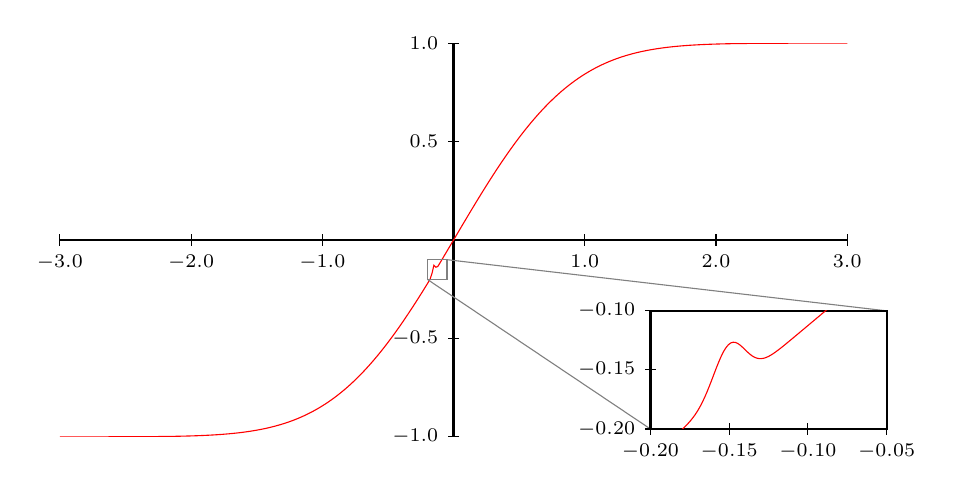
\begin{tikzpicture}
\begin{scope}[shift={(0.0,0.0)}]
\pgfsetxvec{\pgfpoint{1.6666666cm}{0cm}}
\pgfsetyvec{\pgfpoint{0cm}{2.5cm}}
\begin{scope}[shift={(3.0,1.0)}]
\begin{scope}[thick,black,fill=white]
\pgfpathmoveto{ \pgfpointxy {-3.0} {0.0}}
\pgfpathlineto{ \pgfpointxy {3.0} {0.0}}
\pgfpathmoveto{ \pgfpointxy {0.0} {-1.0}}
\pgfpathlineto{ \pgfpointxy {0.0} {1.0}}
\pgfusepath{ stroke, }
\end{scope}
\begin{scope}[yshift=2.5cm]
\draw[] [shift={(-3.0,-1.0)}] (0,2pt) -- (0,-2pt) node[below]{ \scriptsize{\num[round-mode=places,round-precision=1]{-3.0}}};
\draw[] [shift={(-2.0,-1.0)}] (0,2pt) -- (0,-2pt) node[below]{ \scriptsize{\num[round-mode=places,round-precision=1]{-2.0}}};
\draw[] [shift={(-1.0,-1.0)}] (0,2pt) -- (0,-2pt) node[below]{ \scriptsize{\num[round-mode=places,round-precision=1]{-1.0}}};
\draw[] [shift={(1.0,-1.0)}] (0,2pt) -- (0,-2pt) node[below]{ \scriptsize{\num[round-mode=places,round-precision=1]{1.0}}};
\draw[] [shift={(2.0,-1.0)}] (0,2pt) -- (0,-2pt) node[below]{ \scriptsize{\num[round-mode=places,round-precision=1]{2.0}}};
\draw[] [shift={(3.0,-1.0)}] (0,2pt) -- (0,-2pt) node[below]{ \scriptsize{\num[round-mode=places,round-precision=1]{3.0}}};
\end{scope}
\begin{scope}[xshift=5.0cm]
\draw[] [shift={(-3.0,-1.0)}] (2pt,0) -- (-2pt,0) node[left]{ \scriptsize{\num[round-mode=places,round-precision=1]{-1.0}}};
\draw[] [shift={(-3.0,-0.5)}] (2pt,0) -- (-2pt,0) node[left]{ \scriptsize{\num[round-mode=places,round-precision=1]{-0.5}}};
\draw[] [shift={(-3.0,0.5)}] (2pt,0) -- (-2pt,0) node[left]{ \scriptsize{\num[round-mode=places,round-precision=1]{0.5}}};
\draw[] [shift={(-3.0,1.0)}] (2pt,0) -- (-2pt,0) node[left]{ \scriptsize{\num[round-mode=places,round-precision=1]{1.0}}};
\end{scope}
\end{scope}
\pgfsetxvec{\pgfpoint{1cm}{0cm}}
\pgfsetyvec{\pgfpoint{0cm}{1cm}}
\end{scope}
\begin{scope}[]
\pgfpointadd{\pgfpointxy {0.0} {0.0}} {\pgfpoint{0cm}{0cm}}\pgfpathmoveto{ NIL }
\pgfpointadd{\pgfpointxy {0.0} {0.0}} {\pgfpoint{10cm}{0cm}}\pgfpathlineto{ NIL }
\pgfpointadd{\pgfpointxy {0.0} {0.0}} {\pgfpoint{10cm}{5cm}}\pgfpathlineto{ NIL }
\pgfpointadd{\pgfpointxy {0.0} {0.0}} {\pgfpoint{0cm}{5cm}}\pgfpathlineto{ NIL }
\pgfpathclose
\pgfusepath{  clip, }
\begin{scope}[shift={(0.0,0.0)}]
\pgfsetxvec{\pgfpoint{1.6666666cm}{0cm}}
\pgfsetyvec{\pgfpoint{0cm}{2.5cm}}
\begin{scope}[shift={(3.0,1.0)}]
\begin{scope}[red]
\pgfpathmoveto{ \pgfpointxy {-3.0} {-0.9999778948512584}}
\pgfpathlineto{ \pgfpointxy {-2.985} {-0.9999757083350379}}
\pgfpathlineto{ \pgfpointxy {-2.97} {-0.9999733170663182}}
\pgfpathlineto{ \pgfpointxy {-2.955} {-0.9999707029673122}}
\pgfpathlineto{ \pgfpointxy {-2.94} {-0.99996784664559}}
\pgfpathlineto{ \pgfpointxy {-2.925} {-0.9999647269538418}}
\pgfpathlineto{ \pgfpointxy {-2.91} {-0.9999613212537493}}
\pgfpathlineto{ \pgfpointxy {-2.895} {-0.9999576048834065}}
\pgfpathlineto{ \pgfpointxy {-2.88} {-0.9999535514455115}}
\pgfpathlineto{ \pgfpointxy {-2.865} {-0.9999491322368748}}
\pgfpathlineto{ \pgfpointxy {-2.85} {-0.9999443164424575}}
\pgfpathlineto{ \pgfpointxy {-2.835} {-0.9999390709691429}}
\pgfpathlineto{ \pgfpointxy {-2.82} {-0.9999333598509589}}
\pgfpathlineto{ \pgfpointxy {-2.805} {-0.9999271447394446}}
\pgfpathlineto{ \pgfpointxy {-2.79} {-0.9999203839664113}}
\pgfpathlineto{ \pgfpointxy {-2.775} {-0.9999130332073615}}
\pgfpathlineto{ \pgfpointxy {-2.76} {-0.9999050442982494}}
\pgfpathlineto{ \pgfpointxy {-2.745} {-0.9998963658439115}}
\pgfpathlineto{ \pgfpointxy {-2.73} {-0.9998869427777993}}
\pgfpathlineto{ \pgfpointxy {-2.715} {-0.9998767154431919}}
\pgfpathlineto{ \pgfpointxy {-2.7} {-0.999865620549059}}
\pgfpathlineto{ \pgfpointxy {-2.685} {-0.999853589536517}}
\pgfpathlineto{ \pgfpointxy {-2.67} {-0.9998405496871464}}
\pgfpathlineto{ \pgfpointxy {-2.655} {-0.9998264223308793}}
\pgfpathlineto{ \pgfpointxy {-2.64} {-0.9998111241177303}}
\pgfpathlineto{ \pgfpointxy {-2.625} {-0.9997945649944869}}
\pgfpathlineto{ \pgfpointxy {-2.6100001} {-0.9997766495590875}}
\pgfpathlineto{ \pgfpointxy {-2.595} {-0.9997572748749847}}
\pgfpathlineto{ \pgfpointxy {-2.58} {-0.9997363318915964}}
\pgfpathlineto{ \pgfpointxy {-2.565} {-0.9997137040964125}}
\pgfpathlineto{ \pgfpointxy {-2.55} {-0.9996892661202884}}
\pgfpathlineto{ \pgfpointxy {-2.535} {-0.9996628860762126}}
\pgfpathlineto{ \pgfpointxy {-2.52} {-0.9996344214396051}}
\pgfpathlineto{ \pgfpointxy {-2.505} {-0.9996037221103481}}
\pgfpathlineto{ \pgfpointxy {-2.49} {-0.9995706266688278}}
\pgfpathlineto{ \pgfpointxy {-2.475} {-0.9995349645820102}}
\pgfpathlineto{ \pgfpointxy {-2.46} {-0.9994965548342742}}
\pgfpathlineto{ \pgfpointxy {-2.445} {-0.9994552028377658}}
\pgfpathlineto{ \pgfpointxy {-2.43} {-0.9994107046969803}}
\pgfpathlineto{ \pgfpointxy {-2.415} {-0.9993628411831741}}
\pgfpathlineto{ \pgfpointxy {-2.4} {-0.9993113823951093}}
\pgfpathlineto{ \pgfpointxy {-2.385} {-0.9992560815728813}}
\pgfpathlineto{ \pgfpointxy {-2.37} {-0.9991966793596809}}
\pgfpathlineto{ \pgfpointxy {-2.355} {-0.9991329013480114}}
\pgfpathlineto{ \pgfpointxy {-2.3400002} {-0.9990644548790096}}
\pgfpathlineto{ \pgfpointxy {-2.325} {-0.9989910302783986}}
\pgfpathlineto{ \pgfpointxy {-2.31} {-0.9989123017378415}}
\pgfpathlineto{ \pgfpointxy {-2.295} {-0.9988279258631217}}
\pgfpathlineto{ \pgfpointxy {-2.28} {-0.9987375351241278}}
\pgfpathlineto{ \pgfpointxy {-2.265} {-0.9986407474173038}}
\pgfpathlineto{ \pgfpointxy {-2.25} {-0.99853715350349}}
\pgfpathlineto{ \pgfpointxy {-2.2350001} {-0.9984263272279732}}
\pgfpathlineto{ \pgfpointxy {-2.22} {-0.9983078149049633}}
\pgfpathlineto{ \pgfpointxy {-2.205} {-0.9981811409848902}}
\pgfpathlineto{ \pgfpointxy {-2.19} {-0.9980458074115153}}
\pgfpathlineto{ \pgfpointxy {-2.175} {-0.9979012818975463}}
\pgfpathlineto{ \pgfpointxy {-2.16} {-0.9977470154175949}}
\pgfpathlineto{ \pgfpointxy {-2.145} {-0.9975824189686803}}
\pgfpathlineto{ \pgfpointxy {-2.13} {-0.9974068859107228}}
\pgfpathlineto{ \pgfpointxy {-2.115} {-0.9972197680997329}}
\pgfpathlineto{ \pgfpointxy {-2.1} {-0.9970203940990304}}
\pgfpathlineto{ \pgfpointxy {-2.085} {-0.996808059480499}}
\pgfpathlineto{ \pgfpointxy {-2.07} {-0.9965820153161545}}
\pgfpathlineto{ \pgfpointxy {-2.055} {-0.9963414947033638}}
\pgfpathlineto{ \pgfpointxy {-2.04} {-0.9960856759455314}}
\pgfpathlineto{ \pgfpointxy {-2.025} {-0.9958137174811054}}
\pgfpathlineto{ \pgfpointxy {-2.01} {-0.995524721420797}}
\pgfpathlineto{ \pgfpointxy {-1.995} {-0.9952177656037218}}
\pgfpathlineto{ \pgfpointxy {-1.98} {-0.99489187942463}}
\pgfpathlineto{ \pgfpointxy {-1.965} {-0.994546050431862}}
\pgfpathlineto{ \pgfpointxy {-1.95} {-0.9941792216068389}}
\pgfpathlineto{ \pgfpointxy {-1.9350001} {-0.9937902946014261}}
\pgfpathlineto{ \pgfpointxy {-1.9200001} {-0.9933781233472766}}
\pgfpathlineto{ \pgfpointxy {-1.905} {-0.9929415139895813}}
\pgfpathlineto{ \pgfpointxy {-1.89} {-0.9924792268868523}}
\pgfpathlineto{ \pgfpointxy {-1.875} {-0.9919899723248453}}
\pgfpathlineto{ \pgfpointxy {-1.86} {-0.9914724099175326}}
\pgfpathlineto{ \pgfpointxy {-1.845} {-0.9909251512583926}}
\pgfpathlineto{ \pgfpointxy {-1.83} {-0.9903467440356116}}
\pgfpathlineto{ \pgfpointxy {-1.815} {-0.989735694565581}}
\pgfpathlineto{ \pgfpointxy {-1.8000001} {-0.9890904549939443}}
\pgfpathlineto{ \pgfpointxy {-1.7850001} {-0.9884094183935574}}
\pgfpathlineto{ \pgfpointxy {-1.77} {-0.9876909094700103}}
\pgfpathlineto{ \pgfpointxy {-1.755} {-0.9869332261163117}}
\pgfpathlineto{ \pgfpointxy {-1.74} {-0.9861345820588053}}
\pgfpathlineto{ \pgfpointxy {-1.725} {-0.9852931457556806}}
\pgfpathlineto{ \pgfpointxy {-1.71} {-0.9844070163473294}}
\pgfpathlineto{ \pgfpointxy {-1.695} {-0.983474242634905}}
\pgfpathlineto{ \pgfpointxy {-1.6800001} {-0.9824928178594202}}
\pgfpathlineto{ \pgfpointxy {-1.6650001} {-0.9814606593383027}}
\pgfpathlineto{ \pgfpointxy {-1.65} {-0.9803756258274028}}
\pgfpathlineto{ \pgfpointxy {-1.635} {-0.9792355416260458}}
\pgfpathlineto{ \pgfpointxy {-1.62} {-0.9780381505422548}}
\pgfpathlineto{ \pgfpointxy {-1.605} {-0.9767811255765453}}
\pgfpathlineto{ \pgfpointxy {-1.59} {-0.9754620987836773}}
\pgfpathlineto{ \pgfpointxy {-1.575} {-0.974078621731563}}
\pgfpathlineto{ \pgfpointxy {-1.5600001} {-0.972628222882936}}
\pgfpathlineto{ \pgfpointxy {-1.5450001} {-0.9711083262499621}}
\pgfpathlineto{ \pgfpointxy {-1.5300001} {-0.9695163254808733}}
\pgfpathlineto{ \pgfpointxy {-1.515} {-0.967849535554207}}
\pgfpathlineto{ \pgfpointxy {-1.5} {-0.9661052690277371}}
\pgfpathlineto{ \pgfpointxy {-1.485} {-0.9642807155660278}}
\pgfpathlineto{ \pgfpointxy {-1.47} {-0.9623730304958918}}
\pgfpathlineto{ \pgfpointxy {-1.455} {-0.9603793399364072}}
\pgfpathlineto{ \pgfpointxy {-1.44} {-0.9582967104453198}}
\pgfpathlineto{ \pgfpointxy {-1.4250001} {-0.9561221356984225}}
\pgfpathlineto{ \pgfpointxy {-1.4100001} {-0.9538525887297505}}
\pgfpathlineto{ \pgfpointxy {-1.395} {-0.9514849669948426}}
\pgfpathlineto{ \pgfpointxy {-1.38} {-0.9490161689966897}}
\pgfpathlineto{ \pgfpointxy {-1.365} {-0.9464430359161858}}
\pgfpathlineto{ \pgfpointxy {-1.35} {-0.9437623278867372}}
\pgfpathlineto{ \pgfpointxy {-1.335} {-0.9409708392198176}}
\pgfpathlineto{ \pgfpointxy {-1.32} {-0.9380652828235414}}
\pgfpathlineto{ \pgfpointxy {-1.3050001} {-0.9350423680815523}}
\pgfpathlineto{ \pgfpointxy {-1.2900001} {-0.9318987712886478}}
\pgfpathlineto{ \pgfpointxy {-1.2750001} {-0.9286311283734742}}
\pgfpathlineto{ \pgfpointxy {-1.26} {-0.9252360326788243}}
\pgfpathlineto{ \pgfpointxy {-1.245} {-0.9217101983808839}}
\pgfpathlineto{ \pgfpointxy {-1.23} {-0.9180501849922466}}
\pgfpathlineto{ \pgfpointxy {-1.215} {-0.914252606844666}}
\pgfpathlineto{ \pgfpointxy {-1.2} {-0.9103140543342333}}
\pgfpathlineto{ \pgfpointxy {-1.1850001} {-0.906231136031063}}
\pgfpathlineto{ \pgfpointxy {-1.1700001} {-0.9020004509732172}}
\pgfpathlineto{ \pgfpointxy {-1.1550001} {-0.8976186580590639}}
\pgfpathlineto{ \pgfpointxy {-1.14} {-0.8930823419626241}}
\pgfpathlineto{ \pgfpointxy {-1.125} {-0.8883882389404271}}
\pgfpathlineto{ \pgfpointxy {-1.11} {-0.8835329977863016}}
\pgfpathlineto{ \pgfpointxy {-1.095} {-0.8785133386336729}}
\pgfpathlineto{ \pgfpointxy {-1.08} {-0.8733261150730078}}
\pgfpathlineto{ \pgfpointxy {-1.065} {-0.86796807846487}}
\pgfpathlineto{ \pgfpointxy {-1.0500001} {-0.8624360650312175}}
\pgfpathlineto{ \pgfpointxy {-1.0350001} {-0.8567270398733166}}
\pgfpathlineto{ \pgfpointxy {-1.0200001} {-0.8508379783362147}}
\pgfpathlineto{ \pgfpointxy {-1.005} {-0.8447658700356118}}
\pgfpathlineto{ \pgfpointxy {-0.99} {-0.8385079674394238}}
\pgfpathlineto{ \pgfpointxy {-0.97500014} {-0.8320614628677012}}
\pgfpathlineto{ \pgfpointxy {-0.96000004} {-0.8254235234588327}}
\pgfpathlineto{ \pgfpointxy {-0.94499993} {-0.8185916497648636}}
\pgfpathlineto{ \pgfpointxy {-0.93000007} {-0.8115634563869057}}
\pgfpathlineto{ \pgfpointxy {-0.91499996} {-0.804336262350336}}
\pgfpathlineto{ \pgfpointxy {-0.9000001} {-0.7969081202280595}}
\pgfpathlineto{ \pgfpointxy {-0.885} {-0.789276571802554}}
\pgfpathlineto{ \pgfpointxy {-0.8700001} {-0.78143974698542}}
\pgfpathlineto{ \pgfpointxy {-0.855} {-0.7733956338705579}}
\pgfpathlineto{ \pgfpointxy {-0.84000015} {-0.7651426490448335}}
\pgfpathlineto{ \pgfpointxy {-0.82500005} {-0.7566789933233791}}
\pgfpathlineto{ \pgfpointxy {-0.80999994} {-0.7480031197954508}}
\pgfpathlineto{ \pgfpointxy {-0.7950001} {-0.7391140684941908}}
\pgfpathlineto{ \pgfpointxy {-0.78} {-0.7300102937251103}}
\pgfpathlineto{ \pgfpointxy {-0.7650001} {-0.7206912013010431}}
\pgfpathlineto{ \pgfpointxy {-0.75} {-0.7111555786221608}}
\pgfpathlineto{ \pgfpointxy {-0.73500013} {-0.7014031183493686}}
\pgfpathlineto{ \pgfpointxy {-0.72} {-0.6914330469339196}}
\pgfpathlineto{ \pgfpointxy {-0.70500016} {-0.6812455998904763}}
\pgfpathlineto{ \pgfpointxy {-0.69000006} {-0.6708400743317531}}
\pgfpathlineto{ \pgfpointxy {-0.67499995} {-0.660216992866449}}
\pgfpathlineto{ \pgfpointxy {-0.6600001} {-0.649376720897284}}
\pgfpathlineto{ \pgfpointxy {-0.645} {-0.6383196022973859}}
\pgfpathlineto{ \pgfpointxy {-0.6300001} {-0.6270466157637888}}
\pgfpathlineto{ \pgfpointxy {-0.615} {-0.6155582999858287}}
\pgfpathlineto{ \pgfpointxy {-0.60000014} {-0.6038562616818842}}
\pgfpathlineto{ \pgfpointxy {-0.58500004} {-0.5919415719549717}}
\pgfpathlineto{ \pgfpointxy {-0.5700002} {-0.5798160396369354}}
\pgfpathlineto{ \pgfpointxy {-0.55500007} {-0.5674812472817082}}
\pgfpathlineto{ \pgfpointxy {-0.53999996} {-0.5549393902304556}}
\pgfpathlineto{ \pgfpointxy {-0.5250001} {-0.5421928981052622}}
\pgfpathlineto{ \pgfpointxy {-0.51} {-0.5292437727904253}}
\pgfpathlineto{ \pgfpointxy {-0.49500012} {-0.5160952570139519}}
\pgfpathlineto{ \pgfpointxy {-0.48000002} {-0.5027497568965194}}
\pgfpathlineto{ \pgfpointxy {-0.46500015} {-0.4892110189255514}}
\pgfpathlineto{ \pgfpointxy {-0.45000005} {-0.47548189433897914}}
\pgfpathlineto{ \pgfpointxy {-0.43499994} {-0.4615660706751016}}
\pgfpathlineto{ \pgfpointxy {-0.42000008} {-0.44746767196968773}}
\pgfpathlineto{ \pgfpointxy {-0.40499997} {-0.4331903595062201}}
\pgfpathlineto{ \pgfpointxy {-0.3900001} {-0.4187387779686279}}
\pgfpathlineto{ \pgfpointxy {-0.375} {-0.40411692547750133}}
\pgfpathlineto{ \pgfpointxy {-0.36000013} {-0.3893298597736382}}
\pgfpathlineto{ \pgfpointxy {-0.34500003} {-0.37438198778261733}}
\pgfpathlineto{ \pgfpointxy {-0.33000016} {-0.35927874143158567}}
\pgfpathlineto{ \pgfpointxy {-0.31500006} {-0.344025253742944}}
\pgfpathlineto{ \pgfpointxy {-0.29999995} {-0.32862666370740756}}
\pgfpathlineto{ \pgfpointxy {-0.2850001} {-0.31308923451963655}}
\pgfpathlineto{ \pgfpointxy {-0.26999998} {-0.29741806545138383}}
\pgfpathlineto{ \pgfpointxy {-0.2550001} {-0.28161988686270134}}
\pgfpathlineto{ \pgfpointxy {-0.24000001} {-0.2656999893504224}}
\pgfpathlineto{ \pgfpointxy {-0.22500014} {-0.24966535068133797}}
\pgfpathlineto{ \pgfpointxy {-0.21000004} {-0.23352175403526657}}
\pgfpathlineto{ \pgfpointxy {-0.19500017} {-0.21727497267594978}}
\pgfpathlineto{ \pgfpointxy {-0.18000007} {-0.20049248374011114}}
\pgfpathlineto{ \pgfpointxy {-0.16499996} {-0.1715545534363324}}
\pgfpathlineto{ \pgfpointxy {-0.1500001} {-0.128101746018037}}
\pgfpathlineto{ \pgfpointxy {-0.13499999} {-0.13845888038205725}}
\pgfpathlineto{ \pgfpointxy {-0.120000124} {-0.13431510041424086}}
\pgfpathlineto{ \pgfpointxy {-0.10500002} {-0.11804445448569008}}
\pgfpathlineto{ \pgfpointxy {-0.09000015} {-0.10128067264526579}}
\pgfpathlineto{ \pgfpointxy {-0.07500005} {-0.0844703426114842}}
\pgfpathlineto{ \pgfpointxy {-0.06000018} {-0.06762170729321915}}
\pgfpathlineto{ \pgfpointxy {-0.045000076} {-0.050743256652064916}}
\pgfpathlineto{ \pgfpointxy {-0.029999971} {-0.033841389233015606}}
\pgfpathlineto{ \pgfpointxy {-0.015000105} {-0.016924710110142183}}
\pgfpathlineto{ \pgfpointxy {0.0} {0.0}}
\pgfpathlineto{ \pgfpointxy {0.0149998665} {0.016924229511984024}}
\pgfpathlineto{ \pgfpointxy {0.029999971} {0.033841389233015606}}
\pgfpathlineto{ \pgfpointxy {0.044999838} {0.050742828355247016}}
\pgfpathlineto{ \pgfpointxy {0.059999943} {0.0676216806176343}}
\pgfpathlineto{ \pgfpointxy {0.07500005} {0.08447034261150854}}
\pgfpathlineto{ \pgfpointxy {0.089999914} {0.1012806346840418}}
\pgfpathlineto{ \pgfpointxy {0.10500002} {0.11804605287063952}}
\pgfpathlineto{ \pgfpointxy {0.119999886} {0.13475825118828955}}
\pgfpathlineto{ \pgfpointxy {0.13499999} {0.15141060977487186}}
\pgfpathlineto{ \pgfpointxy {0.14999986} {0.16799591733520225}}
\pgfpathlineto{ \pgfpointxy {0.16499996} {0.1845063993453384}}
\pgfpathlineto{ \pgfpointxy {0.17999983} {0.20093559177211362}}
\pgfpathlineto{ \pgfpointxy {0.19499993} {0.21727623707506505}}
\pgfpathlineto{ \pgfpointxy {0.21000004} {0.2335217546428422}}
\pgfpathlineto{ \pgfpointxy {0.2249999} {0.24966501582180067}}
\pgfpathlineto{ \pgfpointxy {0.24000001} {0.2656999893504224}}
\pgfpathlineto{ \pgfpointxy {0.25499988} {0.2816195005360379}}
\pgfpathlineto{ \pgfpointxy {0.26999998} {0.29741806545138383}}
\pgfpathlineto{ \pgfpointxy {0.28499985} {0.3130889008520029}}
\pgfpathlineto{ \pgfpointxy {0.29999995} {0.32862666370740756}}
\pgfpathlineto{ \pgfpointxy {0.31499982} {0.3440248732428789}}
\pgfpathlineto{ \pgfpointxy {0.32999992} {0.3592786406100623}}
\pgfpathlineto{ \pgfpointxy {0.34500003} {0.37438198778261733}}
\pgfpathlineto{ \pgfpointxy {0.3599999} {0.389329754945148}}
\pgfpathlineto{ \pgfpointxy {0.375} {0.40411692547750133}}
\pgfpathlineto{ \pgfpointxy {0.38999987} {0.4187386698735115}}
\pgfpathlineto{ \pgfpointxy {0.40499997} {0.4331903595062201}}
\pgfpathlineto{ \pgfpointxy {0.41999984} {0.44746756131315113}}
\pgfpathlineto{ \pgfpointxy {0.43499994} {0.4615660706751016}}
\pgfpathlineto{ \pgfpointxy {0.4499998} {0.47548161864421723}}
\pgfpathlineto{ \pgfpointxy {0.4649999} {0.4892108289179564}}
\pgfpathlineto{ \pgfpointxy {0.48000002} {0.5027497568965194}}
\pgfpathlineto{ \pgfpointxy {0.4949999} {0.5160949553287273}}
\pgfpathlineto{ \pgfpointxy {0.51} {0.5292437727904253}}
\pgfpathlineto{ \pgfpointxy {0.52499986} {0.5421925651128077}}
\pgfpathlineto{ \pgfpointxy {0.53999996} {0.5549393902304556}}
\pgfpathlineto{ \pgfpointxy {0.5549998} {0.5674810652861666}}
\pgfpathlineto{ \pgfpointxy {0.56999993} {0.5798159254320938}}
\pgfpathlineto{ \pgfpointxy {0.58500004} {0.5919415719549717}}
\pgfpathlineto{ \pgfpointxy {0.5999999} {0.6038561483442308}}
\pgfpathlineto{ \pgfpointxy {0.615} {0.6155582999858287}}
\pgfpathlineto{ \pgfpointxy {0.6299999} {0.6270465037258128}}
\pgfpathlineto{ \pgfpointxy {0.645} {0.6383196022973859}}
\pgfpathlineto{ \pgfpointxy {0.65999985} {0.649376610551735}}
\pgfpathlineto{ \pgfpointxy {0.67499995} {0.660216992866449}}
\pgfpathlineto{ \pgfpointxy {0.6899998} {0.6708398815778611}}
\pgfpathlineto{ \pgfpointxy {0.7049999} {0.6812453575903317}}
\pgfpathlineto{ \pgfpointxy {0.72} {0.6914330469339196}}
\pgfpathlineto{ \pgfpointxy {0.7349999} {0.7014029636276022}}
\pgfpathlineto{ \pgfpointxy {0.75} {0.7111555786221608}}
\pgfpathlineto{ \pgfpointxy {0.76499987} {0.7206910255023738}}
\pgfpathlineto{ \pgfpointxy {0.78} {0.7300102937251103}}
\pgfpathlineto{ \pgfpointxy {0.79499984} {0.7391139248615397}}
\pgfpathlineto{ \pgfpointxy {0.80999994} {0.7480031197954508}}
\pgfpathlineto{ \pgfpointxy {0.8249998} {0.7566788316660754}}
\pgfpathlineto{ \pgfpointxy {0.8399999} {0.7651425549742931}}
\pgfpathlineto{ \pgfpointxy {0.855} {0.7733956338705579}}
\pgfpathlineto{ \pgfpointxy {0.8699999} {0.7814396178160592}}
\pgfpathlineto{ \pgfpointxy {0.885} {0.789276571802554}}
\pgfpathlineto{ \pgfpointxy {0.89999986} {0.7969080330704639}}
\pgfpathlineto{ \pgfpointxy {0.91499996} {0.804336262350336}}
\pgfpathlineto{ \pgfpointxy {0.9299998} {0.8115633196933907}}
\pgfpathlineto{ \pgfpointxy {0.94499993} {0.8185916497648636}}
\pgfpathlineto{ \pgfpointxy {0.9599998} {0.8254234298660563}}
\pgfpathlineto{ \pgfpointxy {0.9749999} {0.8320613366625935}}
\pgfpathlineto{ \pgfpointxy {0.99} {0.8385079674394238}}
\pgfpathlineto{ \pgfpointxy {1.0050001} {0.8447659072313636}}
\pgfpathlineto{ \pgfpointxy {1.02} {0.8508379420619516}}
\pgfpathlineto{ \pgfpointxy {1.0349998} {0.8567269424796609}}
\pgfpathlineto{ \pgfpointxy {1.0499997} {0.8624359359724286}}
\pgfpathlineto{ \pgfpointxy {1.065} {0.86796807846487}}
\pgfpathlineto{ \pgfpointxy {1.0799999} {0.8733260824554839}}
\pgfpathlineto{ \pgfpointxy {1.0949998} {0.8785132752010185}}
\pgfpathlineto{ \pgfpointxy {1.1100001} {0.8835330286086654}}
\pgfpathlineto{ \pgfpointxy {1.125} {0.8883882389404271}}
\pgfpathlineto{ \pgfpointxy {1.1399999} {0.8930823129027041}}
\pgfpathlineto{ \pgfpointxy {1.1549997} {0.8976185536775234}}
\pgfpathlineto{ \pgfpointxy {1.1700001} {0.9020004509732172}}
\pgfpathlineto{ \pgfpointxy {1.185} {0.9062310912367642}}
\pgfpathlineto{ \pgfpointxy {1.1999998} {0.9103140030155119}}
\pgfpathlineto{ \pgfpointxy {1.2149997} {0.9142525323270949}}
\pgfpathlineto{ \pgfpointxy {1.23} {0.9180501849922466}}
\pgfpathlineto{ \pgfpointxy {1.2449999} {0.9217101595865926}}
\pgfpathlineto{ \pgfpointxy {1.2599998} {0.9252359814638371}}
\pgfpathlineto{ \pgfpointxy {1.2750001} {0.9286311283734742}}
\pgfpathlineto{ \pgfpointxy {1.29} {0.9318987503434326}}
\pgfpathlineto{ \pgfpointxy {1.3049998} {0.9350423221332046}}
\pgfpathlineto{ \pgfpointxy {1.3199997} {0.9380652117745992}}
\pgfpathlineto{ \pgfpointxy {1.335} {0.9409708392198176}}
\pgfpathlineto{ \pgfpointxy {1.3499999} {0.9437623097857919}}
\pgfpathlineto{ \pgfpointxy {1.3649998} {0.9464429900460879}}
\pgfpathlineto{ \pgfpointxy {1.3800001} {0.9490161857712673}}
\pgfpathlineto{ \pgfpointxy {1.395} {0.9514849669948426}}
\pgfpathlineto{ \pgfpointxy {1.4099998} {0.9538525480979173}}
\pgfpathlineto{ \pgfpointxy {1.4249997} {0.9561220871401467}}
\pgfpathlineto{ \pgfpointxy {1.44} {0.9582967104453198}}
\pgfpathlineto{ \pgfpointxy {1.4549999} {0.9603793261920363}}
\pgfpathlineto{ \pgfpointxy {1.4699998} {0.9623729961630014}}
\pgfpathlineto{ \pgfpointxy {1.4850001} {0.9642807282124957}}
\pgfpathlineto{ \pgfpointxy {1.5} {0.9661052690277371}}
\pgfpathlineto{ \pgfpointxy {1.5149999} {0.9678495239413245}}
\pgfpathlineto{ \pgfpointxy {1.5299997} {0.9695162855724684}}
\pgfpathlineto{ \pgfpointxy {1.5450001} {0.9711083262499621}}
\pgfpathlineto{ \pgfpointxy {1.56} {0.9726282127024675}}
\pgfpathlineto{ \pgfpointxy {1.5749998} {0.9740786022641214}}
\pgfpathlineto{ \pgfpointxy {1.5899997} {0.9754620655255181}}
\pgfpathlineto{ \pgfpointxy {1.605} {0.9767811255765453}}
\pgfpathlineto{ \pgfpointxy {1.6199999} {0.9780381420597506}}
\pgfpathlineto{ \pgfpointxy {1.6349998} {0.9792355254374719}}
\pgfpathlineto{ \pgfpointxy {1.6500001} {0.9803756335474468}}
\pgfpathlineto{ \pgfpointxy {1.665} {0.981460651978796}}
\pgfpathlineto{ \pgfpointxy {1.6799998} {0.9824928038346491}}
\pgfpathlineto{ \pgfpointxy {1.6949997} {0.9834742225997524}}
\pgfpathlineto{ \pgfpointxy {1.71} {0.9844070163473294}}
\pgfpathlineto{ \pgfpointxy {1.7249999} {0.985293136392341}}
\pgfpathlineto{ \pgfpointxy {1.7399998} {0.9861345683378413}}
\pgfpathlineto{ \pgfpointxy {1.7550001} {0.9869332315837704}}
\pgfpathlineto{ \pgfpointxy {1.77} {0.9876909094700103}}
\pgfpathlineto{ \pgfpointxy {1.7849998} {0.9884094058789614}}
\pgfpathlineto{ \pgfpointxy {1.7999997} {0.9890904409483297}}
\pgfpathlineto{ \pgfpointxy {1.815} {0.989735694565581}}
\pgfpathlineto{ \pgfpointxy {1.8299999} {0.9903467375946742}}
\pgfpathlineto{ \pgfpointxy {1.8449998} {0.9909251411719724}}
\pgfpathlineto{ \pgfpointxy {1.8599997} {0.9914723965900984}}
\pgfpathlineto{ \pgfpointxy {1.875} {0.9919899723248453}}
\pgfpathlineto{ \pgfpointxy {1.8899999} {0.9924792217377774}}
\pgfpathlineto{ \pgfpointxy {1.9049997} {0.9929415047501007}}
\pgfpathlineto{ \pgfpointxy {1.9200001} {0.9933781233472766}}
\pgfpathlineto{ \pgfpointxy {1.935} {0.9937902917366402}}
\pgfpathlineto{ \pgfpointxy {1.9499998} {0.9941792156259124}}
\pgfpathlineto{ \pgfpointxy {1.9649997} {0.9945460418505943}}
\pgfpathlineto{ \pgfpointxy {1.98} {0.99489187942463}}
\pgfpathlineto{ \pgfpointxy {1.9949999} {0.9952177633290752}}
\pgfpathlineto{ \pgfpointxy {2.0099998} {0.9955247160567203}}
\pgfpathlineto{ \pgfpointxy {2.025} {0.9958137174811054}}
\pgfpathlineto{ \pgfpointxy {2.04} {0.9960856759455314}}
\pgfpathlineto{ \pgfpointxy {2.0549998} {0.9963414911183914}}
\pgfpathlineto{ \pgfpointxy {2.0699997} {0.9965820119424215}}
\pgfpathlineto{ \pgfpointxy {2.085} {0.996808059480499}}
\pgfpathlineto{ \pgfpointxy {2.1} {0.9970203940990304}}
\pgfpathlineto{ \pgfpointxy {2.1149998} {0.9972197652958383}}
\pgfpathlineto{ \pgfpointxy {2.13} {0.9974068859107228}}
\pgfpathlineto{ \pgfpointxy {2.145} {0.9975824189686803}}
\pgfpathlineto{ \pgfpointxy {2.1599998} {0.9977470130970911}}
\pgfpathlineto{ \pgfpointxy {2.1749997} {0.9979012797209211}}
\pgfpathlineto{ \pgfpointxy {2.19} {0.9980458074115153}}
\pgfpathlineto{ \pgfpointxy {2.205} {0.9981811409848902}}
\pgfpathlineto{ \pgfpointxy {2.2199998} {0.9983078129394373}}
\pgfpathlineto{ \pgfpointxy {2.2349997} {0.998426323873746}}
\pgfpathlineto{ \pgfpointxy {2.25} {0.99853715350349}}
\pgfpathlineto{ \pgfpointxy {2.2649999} {0.9986407459492611}}
\pgfpathlineto{ \pgfpointxy {2.2799997} {0.9987375334316094}}
\pgfpathlineto{ \pgfpointxy {2.295} {0.9988279258631217}}
\pgfpathlineto{ \pgfpointxy {2.31} {0.9989123017378415}}
\pgfpathlineto{ \pgfpointxy {2.3249998} {0.9989910289778833}}
\pgfpathlineto{ \pgfpointxy {2.3399997} {0.9990644527912469}}
\pgfpathlineto{ \pgfpointxy {2.355} {0.9991329013480114}}
\pgfpathlineto{ \pgfpointxy {2.37} {0.9991966793596809}}
\pgfpathlineto{ \pgfpointxy {2.3849998} {0.9992560806478697}}
\pgfpathlineto{ \pgfpointxy {2.4} {0.9993113823951093}}
\pgfpathlineto{ \pgfpointxy {2.415} {0.9993628411831741}}
\pgfpathlineto{ \pgfpointxy {2.4299998} {0.9994107039058351}}
\pgfpathlineto{ \pgfpointxy {2.4449997} {0.9994552020602632}}
\pgfpathlineto{ \pgfpointxy {2.46} {0.9994965548342742}}
\pgfpathlineto{ \pgfpointxy {2.475} {0.9995349645820102}}
\pgfpathlineto{ \pgfpointxy {2.4899998} {0.9995706260459392}}
\pgfpathlineto{ \pgfpointxy {2.505} {0.9996037221103481}}
\pgfpathlineto{ \pgfpointxy {2.52} {0.9996344214396051}}
\pgfpathlineto{ \pgfpointxy {2.5349998} {0.9996628856687151}}
\pgfpathlineto{ \pgfpointxy {2.5499997} {0.999689265742456}}
\pgfpathlineto{ \pgfpointxy {2.565} {0.9997137040964125}}
\pgfpathlineto{ \pgfpointxy {2.58} {0.9997363318915964}}
\pgfpathlineto{ \pgfpointxy {2.5949998} {0.9997572745746383}}
\pgfpathlineto{ \pgfpointxy {2.6099997} {0.9997766489430951}}
\pgfpathlineto{ \pgfpointxy {2.625} {0.9997945649944869}}
\pgfpathlineto{ \pgfpointxy {2.6399999} {0.9998111238799637}}
\pgfpathlineto{ \pgfpointxy {2.6549997} {0.9998264221111294}}
\pgfpathlineto{ \pgfpointxy {2.67} {0.9998405496871464}}
\pgfpathlineto{ \pgfpointxy {2.685} {0.999853589536517}}
\pgfpathlineto{ \pgfpointxy {2.6999998} {0.9998656203760506}}
\pgfpathlineto{ \pgfpointxy {2.7149997} {0.999876715283586}}
\pgfpathlineto{ \pgfpointxy {2.73} {0.9998869427777993}}
\pgfpathlineto{ \pgfpointxy {2.745} {0.9998963658439115}}
\pgfpathlineto{ \pgfpointxy {2.7599998} {0.9999050441625038}}
\pgfpathlineto{ \pgfpointxy {2.775} {0.9999130332073615}}
\pgfpathlineto{ \pgfpointxy {2.79} {0.9999203839664113}}
\pgfpathlineto{ \pgfpointxy {2.8049998} {0.9999271446419986}}
\pgfpathlineto{ \pgfpointxy {2.8199997} {0.9999333597482575}}
\pgfpathlineto{ \pgfpointxy {2.835} {0.9999390709691429}}
\pgfpathlineto{ \pgfpointxy {2.85} {0.9999443164424575}}
\pgfpathlineto{ \pgfpointxy {2.8649998} {0.9999491321430637}}
\pgfpathlineto{ \pgfpointxy {2.8799996} {0.9999535513179366}}
\pgfpathlineto{ \pgfpointxy {2.895} {0.9999576048834065}}
\pgfpathlineto{ \pgfpointxy {2.9099998} {0.9999613212000787}}
\pgfpathlineto{ \pgfpointxy {2.9249997} {0.9999647268975985}}
\pgfpathlineto{ \pgfpointxy {2.94} {0.99996784664559}}
\pgfpathlineto{ \pgfpointxy {2.955} {0.9999707029673122}}
\pgfpathlineto{ \pgfpointxy {2.9699998} {0.9999733170285297}}
\pgfpathlineto{ \pgfpointxy {2.9849997} {0.9999757082955643}}
\pgfpathlineto{ \pgfpointxy {3.0} {0.9999778948512584}}
\pgfusepath{ stroke, }
\end{scope}
\end{scope}
\pgfsetxvec{\pgfpoint{1cm}{0cm}}
\pgfsetyvec{\pgfpoint{0cm}{1cm}}
\end{scope}
\end{scope}
\begin{scope}[gray]
\begin{scope}[shift={(0.0,0.0)}]
\pgfsetxvec{\pgfpoint{1.6666666cm}{0cm}}
\pgfsetyvec{\pgfpoint{0cm}{2.5cm}}
\begin{scope}[shift={(3.0,1.0)}]
\pgfpathmoveto{ \pgfpointxy {-0.2} {-0.2}}
\pgfpathlineto{ \pgfpointxy {-0.05} {-0.2}}
\pgfpathlineto{ \pgfpointxy {-0.05} {-0.1}}
\pgfpathlineto{ \pgfpointxy {-0.2} {-0.1}}
\pgfpathclose
\end{scope}
\pgfsetxvec{\pgfpoint{1cm}{0cm}}
\pgfsetyvec{\pgfpoint{0cm}{1cm}}
\end{scope}
\pgfusepath{ stroke, }
\pgfseteorule
\begin{scope}[shift={(7.5,0.1)}]
\pgfsetxvec{\pgfpoint{20.0cm}{0cm}}
\pgfsetyvec{\pgfpoint{0cm}{15.0cm}}
\begin{scope}[shift={(0.2,0.2)}]
\pgfpathmoveto{ \pgfpointxy {-0.2} {-0.2}}
\pgfpathlineto{ \pgfpointxy {-0.05} {-0.2}}
\pgfpathlineto{ \pgfpointxy {-0.05} {-0.1}}
\pgfpathlineto{ \pgfpointxy {-0.2} {-0.1}}
\pgfpathclose
\end{scope}
\pgfsetxvec{\pgfpoint{1cm}{0cm}}
\pgfsetyvec{\pgfpoint{0cm}{1cm}}
\end{scope}
\begin{scope}[shift={(0.0,0.0)}]
\pgfsetxvec{\pgfpoint{1.6666666cm}{0cm}}
\pgfsetyvec{\pgfpoint{0cm}{2.5cm}}
\begin{scope}[shift={(3.0,1.0)}]
\pgfpathmoveto{ \pgfpointxy {-0.2} {-0.2}}
\pgfpathlineto{ \pgfpointxy {-0.05} {-0.2}}
\pgfpathlineto{ \pgfpointxy {-0.05} {-0.1}}
\pgfpathlineto{ \pgfpointxy {-0.2} {-0.1}}
\pgfpathclose
\end{scope}
\pgfsetxvec{\pgfpoint{1cm}{0cm}}
\pgfsetyvec{\pgfpoint{0cm}{1cm}}
\end{scope}
\pgfpathmoveto{ \pgfpointxy {0.0} {0.0}}
\pgfpathlineto{ \pgfpointxy {10.5} {0.0}}
\pgfpathlineto{ \pgfpointxy {10.5} {5.0}}
\pgfpathlineto{ \pgfpointxy {0.0} {5.0}}
\pgfpathclose
\pgfusepath{  clip, }
\pgfpathmoveto{ \pgfpointxy {4.6666665} {2.0}}
\pgfpathlineto{ \pgfpointxy {7.5} {0.1}}
\pgfpathmoveto{ \pgfpointxy {4.9166665} {2.25}}
\pgfpathlineto{ \pgfpointxy {10.5} {1.6}}
\pgfusepath{ stroke, }
\end{scope}
\begin{scope}[shift={(7.5,0.1)}]
\pgfsetxvec{\pgfpoint{20.0cm}{0cm}}
\pgfsetyvec{\pgfpoint{0cm}{15.0cm}}
\begin{scope}[shift={(0.2,0.2)}]
\begin{scope}[thick,black,fill=white]
\pgfpathmoveto{ \pgfpointxy {-0.2} {-0.2}}
\pgfpathlineto{ \pgfpointxy {-0.05} {-0.2}}
\pgfpathlineto{ \pgfpointxy {-0.05} {-0.1}}
\pgfpathlineto{ \pgfpointxy {-0.2} {-0.1}}
\pgfpathclose
\pgfusepath{ stroke, fill, }
\end{scope}
\begin{scope}[yshift=0cm]
\draw[] [shift={(-0.19999999,-0.2)}] (0,2pt) -- (0,-2pt) node[below]{ \scriptsize{\num[round-mode=places,round-precision=2]{-0.19999999}}};
\draw[] [shift={(-0.14999999,-0.2)}] (0,2pt) -- (0,-2pt) node[below]{ \scriptsize{\num[round-mode=places,round-precision=2]{-0.14999999}}};
\draw[] [shift={(-0.099999994,-0.2)}] (0,2pt) -- (0,-2pt) node[below]{ \scriptsize{\num[round-mode=places,round-precision=2]{-0.099999994}}};
\draw[] [shift={(-0.049999997,-0.2)}] (0,2pt) -- (0,-2pt) node[below]{ \scriptsize{\num[round-mode=places,round-precision=2]{-0.049999997}}};
\end{scope}
\begin{scope}[xshift=0cm]
\draw[] [shift={(-0.2,-0.19999999)}] (2pt,0) -- (-2pt,0) node[left]{ \scriptsize{\num[round-mode=places,round-precision=2]{-0.19999999}}};
\draw[] [shift={(-0.2,-0.14999999)}] (2pt,0) -- (-2pt,0) node[left]{ \scriptsize{\num[round-mode=places,round-precision=2]{-0.14999999}}};
\draw[] [shift={(-0.2,-0.099999994)}] (2pt,0) -- (-2pt,0) node[left]{ \scriptsize{\num[round-mode=places,round-precision=2]{-0.099999994}}};
\end{scope}
\end{scope}
\pgfsetxvec{\pgfpoint{1cm}{0cm}}
\pgfsetyvec{\pgfpoint{0cm}{1cm}}
\end{scope}
\begin{scope}[]
\pgfpointadd{\pgfpointxy {0.0} {0.0}} {\pgfpoint{7.5cm}{0.1cm}}\pgfpathmoveto{ NIL }
\pgfpointadd{\pgfpointxy {0.0} {0.0}} {\pgfpoint{10.5cm}{0.1cm}}\pgfpathlineto{ NIL }
\pgfpointadd{\pgfpointxy {0.0} {0.0}} {\pgfpoint{10.5cm}{1.6cm}}\pgfpathlineto{ NIL }
\pgfpointadd{\pgfpointxy {0.0} {0.0}} {\pgfpoint{7.5cm}{1.6cm}}\pgfpathlineto{ NIL }
\pgfpathclose
\pgfusepath{  clip, }
\begin{scope}[shift={(7.5,0.1)}]
\pgfsetxvec{\pgfpoint{20.0cm}{0cm}}
\pgfsetyvec{\pgfpoint{0cm}{15.0cm}}
\begin{scope}[shift={(0.2,0.2)}]
\begin{scope}[red]
\pgfpathmoveto{ \pgfpointxy {-0.2} {-0.22270238754219424}}
\pgfpathlineto{ \pgfpointxy {-0.1985} {-0.22107553402496863}}
\pgfpathlineto{ \pgfpointxy {-0.197} {-0.21944764979042922}}
\pgfpathlineto{ \pgfpointxy {-0.1955} {-0.2178181354748758}}
\pgfpathlineto{ \pgfpointxy {-0.194} {-0.21618730409531084}}
\pgfpathlineto{ \pgfpointxy {-0.1925} {-0.21455448023347773}}
\pgfpathlineto{ \pgfpointxy {-0.191} {-0.2129188083395523}}
\pgfpathlineto{ \pgfpointxy {-0.1895} {-0.2112790942536496}}
\pgfpathlineto{ \pgfpointxy {-0.18800001} {-0.20963285536454224}}
\pgfpathlineto{ \pgfpointxy {-0.1865} {-0.20797690708662173}}
\pgfpathlineto{ \pgfpointxy {-0.185} {-0.20630545834553085}}
\pgfpathlineto{ \pgfpointxy {-0.1835} {-0.20461076678323512}}
\pgfpathlineto{ \pgfpointxy {-0.18200001} {-0.2028812469755061}}
\pgfpathlineto{ \pgfpointxy {-0.1805} {-0.2011007502960706}}
\pgfpathlineto{ \pgfpointxy {-0.179} {-0.1992479460690563}}
\pgfpathlineto{ \pgfpointxy {-0.17750001} {-0.19729413322754916}}
\pgfpathlineto{ \pgfpointxy {-0.176} {-0.19520467717056103}}
\pgfpathlineto{ \pgfpointxy {-0.1745} {-0.19293795213598208}}
\pgfpathlineto{ \pgfpointxy {-0.17300001} {-0.19044671221058546}}
\pgfpathlineto{ \pgfpointxy {-0.1715} {-0.18768131559381832}}
\pgfpathlineto{ \pgfpointxy {-0.17} {-0.1845933473308297}}
\pgfpathlineto{ \pgfpointxy {-0.1685} {-0.1811412945100708}}
\pgfpathlineto{ \pgfpointxy {-0.167} {-0.1772971446628447}}
\pgfpathlineto{ \pgfpointxy {-0.1655} {-0.1730547997547754}}
\pgfpathlineto{ \pgfpointxy {-0.164} {-0.1684354753729975}}
\pgfpathlineto{ \pgfpointxy {-0.1625} {-0.1634952841298452}}
\pgfpathlineto{ \pgfpointxy {-0.161} {-0.15832604627558092}}
\pgfpathlineto{ \pgfpointxy {-0.1595} {-0.15305560962069487}}
\pgfpathlineto{ \pgfpointxy {-0.158} {-0.14784197551623554}}
\pgfpathlineto{ \pgfpointxy {-0.15650001} {-0.1428627190966561}}
\pgfpathlineto{ \pgfpointxy {-0.155} {-0.13830143396387004}}
\pgfpathlineto{ \pgfpointxy {-0.1535} {-0.1343311595913951}}
\pgfpathlineto{ \pgfpointxy {-0.15200001} {-0.13109744973711734}}
\pgfpathlineto{ \pgfpointxy {-0.1505} {-0.1287030511344668}}
\pgfpathlineto{ \pgfpointxy {-0.149} {-0.1271971955645439}}
\pgfpathlineto{ \pgfpointxy {-0.14750001} {-0.1265698760407636}}
\pgfpathlineto{ \pgfpointxy {-0.146} {-0.1267532822279401}}
\pgfpathlineto{ \pgfpointxy {-0.1445} {-0.12762859520227054}}
\pgfpathlineto{ \pgfpointxy {-0.143} {-0.12903976674269052}}
\pgfpathlineto{ \pgfpointxy {-0.1415} {-0.13080811094198683}}
\pgfpathlineto{ \pgfpointxy {-0.14} {-0.13274990670907053}}
\pgfpathlineto{ \pgfpointxy {-0.1385} {-0.1346934860117297}}
\pgfpathlineto{ \pgfpointxy {-0.137} {-0.13648957779420356}}
\pgfpathlineto{ \pgfpointxy {-0.1355} {-0.1380215212191859}}
\pgfpathlineto{ \pgfpointxy {-0.134} {-0.1392102637431023}}
\pgfpathlineto{ \pgfpointxy {-0.1325} {-0.14001205196010424}}
\pgfpathlineto{ \pgfpointxy {-0.13100001} {-0.14041476499044223}}
\pgfpathlineto{ \pgfpointxy {-0.1295} {-0.14043313454162928}}
\pgfpathlineto{ \pgfpointxy {-0.128} {-0.1400999298376061}}
\pgfpathlineto{ \pgfpointxy {-0.12650001} {-0.1394602675682118}}
\pgfpathlineto{ \pgfpointxy {-0.125} {-0.1385632350577173}}
\pgfpathlineto{ \pgfpointxy {-0.123500004} {-0.13745831602435502}}
\pgfpathlineto{ \pgfpointxy {-0.122} {-0.13619077186711434}}
\pgfpathlineto{ \pgfpointxy {-0.120500006} {-0.13480019580347946}}
\pgfpathlineto{ \pgfpointxy {-0.119} {-0.13331924718317165}}
\pgfpathlineto{ \pgfpointxy {-0.1175} {-0.13177405431423847}}
\pgfpathlineto{ \pgfpointxy {-0.116000004} {-0.1301840663471346}}
\pgfpathlineto{ \pgfpointxy {-0.1145} {-0.12856392887977672}}
\pgfpathlineto{ \pgfpointxy {-0.113000005} {-0.12692397574822226}}
\pgfpathlineto{ \pgfpointxy {-0.1115} {-0.12527081125812523}}
\pgfpathlineto{ \pgfpointxy {-0.11} {-0.12360964619074881}}
\pgfpathlineto{ \pgfpointxy {-0.108500004} {-0.12194329562338416}}
\pgfpathlineto{ \pgfpointxy {-0.107} {-0.12027378277232485}}
\pgfpathlineto{ \pgfpointxy {-0.105500005} {-0.11860205627944291}}
\pgfpathlineto{ \pgfpointxy {-0.104} {-0.1169285303348311}}
\pgfpathlineto{ \pgfpointxy {-0.1025} {-0.11525434904973468}}
\pgfpathlineto{ \pgfpointxy {-0.101} {-0.11357969387878089}}
\pgfpathlineto{ \pgfpointxy {-0.0995} {-0.11190418928571777}}
\pgfpathlineto{ \pgfpointxy {-0.098000005} {-0.11022808801748528}}
\pgfpathlineto{ \pgfpointxy {-0.0965} {-0.1085513756694257}}
\pgfpathlineto{ \pgfpointxy {-0.095} {-0.10687437133283736}}
\pgfpathlineto{ \pgfpointxy {-0.0935} {-0.10519698505651184}}
\pgfpathlineto{ \pgfpointxy {-0.092} {-0.10351877658689634}}
\pgfpathlineto{ \pgfpointxy {-0.090500005} {-0.1018403382601793}}
\pgfpathlineto{ \pgfpointxy {-0.089} {-0.10016139184315438}}
\pgfpathlineto{ \pgfpointxy {-0.0875} {-0.09848184540114868}}
\pgfpathlineto{ \pgfpointxy {-0.086} {-0.09680211075997687}}
\pgfpathlineto{ \pgfpointxy {-0.0845} {-0.09512174480361839}}
\pgfpathlineto{ \pgfpointxy {-0.083000004} {-0.09344105235586839}}
\pgfpathlineto{ \pgfpointxy {-0.0815} {-0.09175992877755566}}
\pgfpathlineto{ \pgfpointxy {-0.08} {-0.09007827678922334}}
\pgfpathlineto{ \pgfpointxy {-0.0785} {-0.0883963410989217}}
\pgfpathlineto{ \pgfpointxy {-0.077} {-0.08671407706325038}}
\pgfpathlineto{ \pgfpointxy {-0.075500004} {-0.08503133047049154}}
\pgfpathlineto{ \pgfpointxy {-0.074} {-0.08334782850280631}}
\pgfpathlineto{ \pgfpointxy {-0.072500005} {-0.08166433076438322}}
\pgfpathlineto{ \pgfpointxy {-0.070999995} {-0.07998033440837303}}
\pgfpathlineto{ \pgfpointxy {-0.0695} {-0.07829632038709}}
\pgfpathlineto{ \pgfpointxy {-0.068} {-0.07661166605726245}}
\pgfpathlineto{ \pgfpointxy {-0.06650001} {-0.07492684889819698}}
\pgfpathlineto{ \pgfpointxy {-0.065} {-0.07324165206968068}}
\pgfpathlineto{ \pgfpointxy {-0.0635} {-0.07155597807929459}}
\pgfpathlineto{ \pgfpointxy {-0.062000006} {-0.0698701294449744}}
\pgfpathlineto{ \pgfpointxy {-0.060499996} {-0.06818394713616127}}
\pgfpathlineto{ \pgfpointxy {-0.059} {-0.06649733335952268}}
\pgfpathlineto{ \pgfpointxy {-0.057500005} {-0.06481041667162912}}
\pgfpathlineto{ \pgfpointxy {-0.05600001} {-0.06312333081802479}}
\pgfpathlineto{ \pgfpointxy {-0.0545} {-0.06143597179850957}}
\pgfpathlineto{ \pgfpointxy {-0.053000003} {-0.05974835978322235}}
\pgfpathlineto{ \pgfpointxy {-0.051500008} {-0.058060450364861405}}
\pgfpathlineto{ \pgfpointxy {-0.049999997} {-0.056372082202142515}}
\pgfusepath{ stroke, }
\end{scope}
\end{scope}
\pgfsetxvec{\pgfpoint{1cm}{0cm}}
\pgfsetyvec{\pgfpoint{0cm}{1cm}}
\end{scope}
\end{scope}
\end{tikzpicture}
\end{document}

  \caption{ Zooming in on region. }
\end{figure}

\begin{figure}[H]
  \centering
  %%% AUTO GENERATED CODE
\documentclass{standalone}
\ifx\HCode\UnDef\else\def\pgfsysdriver{pgfsys-tex4ht.def}\fi
\usepackage[usenames,dvipsnames,svgnames,table]{xcolor}
\usepackage{tikz}
\usepackage{color}
\usepackage{siunitx}
\usetikzlibrary{arrows,shapes}
\begin{document}
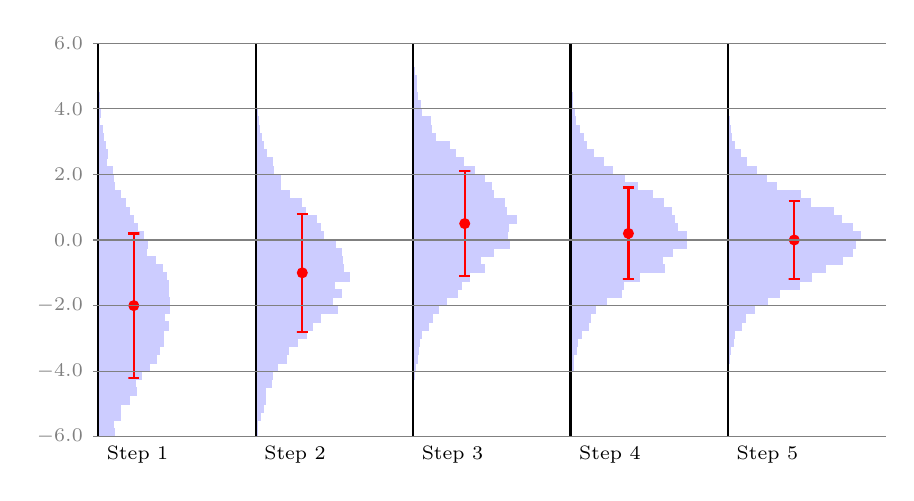
\begin{tikzpicture}[]
\begin{scope}[shift={(0.0,0.0)}]
\pgfsetxvec{\pgfpoint{0.002cm}{0cm}}
\pgfsetyvec{\pgfpoint{0cm}{0.41666666cm}}
\begin{scope}[shift={(-0.0,6.0)}]
\begin{scope}[fill=blue!20,draw=blue!20]
\pgfpathmoveto{ \pgfpointxy {0.0} {6.0}}
\pgfpathlineto{ \pgfpointxy {0.0} {6.0}}
\pgfpathlineto{ \pgfpointxy {0.0} {6.0}}
\pgfpathlineto{ \pgfpointxy {0.0} {5.75}}
\pgfpathlineto{ \pgfpointxy {1.0} {5.75}}
\pgfpathlineto{ \pgfpointxy {1.0} {5.5}}
\pgfpathlineto{ \pgfpointxy {0.0} {5.5}}
\pgfpathlineto{ \pgfpointxy {0.0} {5.25}}
\pgfpathlineto{ \pgfpointxy {2.0} {5.25}}
\pgfpathlineto{ \pgfpointxy {2.0} {5.0}}
\pgfpathlineto{ \pgfpointxy {5.0} {5.0}}
\pgfpathlineto{ \pgfpointxy {5.0} {4.75}}
\pgfpathlineto{ \pgfpointxy {5.0} {4.75}}
\pgfpathlineto{ \pgfpointxy {5.0} {4.5}}
\pgfpathlineto{ \pgfpointxy {8.0} {4.5}}
\pgfpathlineto{ \pgfpointxy {8.0} {4.25}}
\pgfpathlineto{ \pgfpointxy {9.0} {4.25}}
\pgfpathlineto{ \pgfpointxy {9.0} {4.0}}
\pgfpathlineto{ \pgfpointxy {12.0} {4.0}}
\pgfpathlineto{ \pgfpointxy {12.0} {3.75}}
\pgfpathlineto{ \pgfpointxy {9.0} {3.75}}
\pgfpathlineto{ \pgfpointxy {9.0} {3.5}}
\pgfpathlineto{ \pgfpointxy {28.0} {3.5}}
\pgfpathlineto{ \pgfpointxy {28.0} {3.25}}
\pgfpathlineto{ \pgfpointxy {35.0} {3.25}}
\pgfpathlineto{ \pgfpointxy {35.0} {3.0}}
\pgfpathlineto{ \pgfpointxy {45.0} {3.0}}
\pgfpathlineto{ \pgfpointxy {45.0} {2.75}}
\pgfpathlineto{ \pgfpointxy {58.0} {2.75}}
\pgfpathlineto{ \pgfpointxy {58.0} {2.5}}
\pgfpathlineto{ \pgfpointxy {53.0} {2.5}}
\pgfpathlineto{ \pgfpointxy {53.0} {2.25}}
\pgfpathlineto{ \pgfpointxy {90.0} {2.25}}
\pgfpathlineto{ \pgfpointxy {90.0} {2.0}}
\pgfpathlineto{ \pgfpointxy {95.0} {2.0}}
\pgfpathlineto{ \pgfpointxy {95.0} {1.75}}
\pgfpathlineto{ \pgfpointxy {102.0} {1.75}}
\pgfpathlineto{ \pgfpointxy {102.0} {1.5}}
\pgfpathlineto{ \pgfpointxy {144.0} {1.5}}
\pgfpathlineto{ \pgfpointxy {144.0} {1.25}}
\pgfpathlineto{ \pgfpointxy {175.0} {1.25}}
\pgfpathlineto{ \pgfpointxy {175.0} {1.0}}
\pgfpathlineto{ \pgfpointxy {202.0} {1.0}}
\pgfpathlineto{ \pgfpointxy {202.0} {0.75}}
\pgfpathlineto{ \pgfpointxy {224.0} {0.75}}
\pgfpathlineto{ \pgfpointxy {224.0} {0.5}}
\pgfpathlineto{ \pgfpointxy {250.0} {0.5}}
\pgfpathlineto{ \pgfpointxy {250.0} {0.25}}
\pgfpathlineto{ \pgfpointxy {285.0} {0.25}}
\pgfpathlineto{ \pgfpointxy {285.0} {0.0}}
\pgfpathlineto{ \pgfpointxy {316.0} {0.0}}
\pgfpathlineto{ \pgfpointxy {316.0} {-0.25}}
\pgfpathlineto{ \pgfpointxy {306.0} {-0.25}}
\pgfpathlineto{ \pgfpointxy {306.0} {-0.5}}
\pgfpathlineto{ \pgfpointxy {362.0} {-0.5}}
\pgfpathlineto{ \pgfpointxy {362.0} {-0.75}}
\pgfpathlineto{ \pgfpointxy {406.0} {-0.75}}
\pgfpathlineto{ \pgfpointxy {406.0} {-1.0}}
\pgfpathlineto{ \pgfpointxy {434.0} {-1.0}}
\pgfpathlineto{ \pgfpointxy {434.0} {-1.25}}
\pgfpathlineto{ \pgfpointxy {445.0} {-1.25}}
\pgfpathlineto{ \pgfpointxy {445.0} {-1.5}}
\pgfpathlineto{ \pgfpointxy {447.0} {-1.5}}
\pgfpathlineto{ \pgfpointxy {447.0} {-1.75}}
\pgfpathlineto{ \pgfpointxy {453.0} {-1.75}}
\pgfpathlineto{ \pgfpointxy {453.0} {-2.0}}
\pgfpathlineto{ \pgfpointxy {453.0} {-2.0}}
\pgfpathlineto{ \pgfpointxy {453.0} {-2.25}}
\pgfpathlineto{ \pgfpointxy {422.0} {-2.25}}
\pgfpathlineto{ \pgfpointxy {422.0} {-2.5}}
\pgfpathlineto{ \pgfpointxy {447.0} {-2.5}}
\pgfpathlineto{ \pgfpointxy {447.0} {-2.75}}
\pgfpathlineto{ \pgfpointxy {414.0} {-2.75}}
\pgfpathlineto{ \pgfpointxy {414.0} {-3.0}}
\pgfpathlineto{ \pgfpointxy {413.0} {-3.0}}
\pgfpathlineto{ \pgfpointxy {413.0} {-3.25}}
\pgfpathlineto{ \pgfpointxy {391.0} {-3.25}}
\pgfpathlineto{ \pgfpointxy {391.0} {-3.5}}
\pgfpathlineto{ \pgfpointxy {368.0} {-3.5}}
\pgfpathlineto{ \pgfpointxy {368.0} {-3.75}}
\pgfpathlineto{ \pgfpointxy {323.0} {-3.75}}
\pgfpathlineto{ \pgfpointxy {323.0} {-4.0}}
\pgfpathlineto{ \pgfpointxy {278.0} {-4.0}}
\pgfpathlineto{ \pgfpointxy {278.0} {-4.25}}
\pgfpathlineto{ \pgfpointxy {237.0} {-4.25}}
\pgfpathlineto{ \pgfpointxy {237.0} {-4.5}}
\pgfpathlineto{ \pgfpointxy {242.0} {-4.5}}
\pgfpathlineto{ \pgfpointxy {242.0} {-4.75}}
\pgfpathlineto{ \pgfpointxy {197.0} {-4.75}}
\pgfpathlineto{ \pgfpointxy {197.0} {-5.0}}
\pgfpathlineto{ \pgfpointxy {143.0} {-5.0}}
\pgfpathlineto{ \pgfpointxy {143.0} {-5.25}}
\pgfpathlineto{ \pgfpointxy {143.0} {-5.25}}
\pgfpathlineto{ \pgfpointxy {143.0} {-5.5}}
\pgfpathlineto{ \pgfpointxy {99.0} {-5.5}}
\pgfpathlineto{ \pgfpointxy {99.0} {-5.75}}
\pgfpathlineto{ \pgfpointxy {103.0} {-5.75}}
\pgfpathlineto{ \pgfpointxy {103.0} {-6.0}}
\pgfpathlineto{ \pgfpointxy {0.0} {-6.0}}
\pgfusepath{ stroke, fill, }
\end{scope}
\draw[thick,black] (0.0,-6.0) -- (0.0,6.0);
\begin{scope}[red,fill=red,thick]
\pgfpathmoveto{ \pgfpointadd{\pgfpointxy {226.5} {0.20000005}} {\pgfpoint{-2pt}{0}} }
\pgfpathlineto{ \pgfpointadd{\pgfpointxy {226.5} {0.20000005}} {\pgfpoint{2pt}{0}} }
\pgfpathlineto{ \pgfpointadd{\pgfpointxy {226.5} {0.20000005}} {\pgfpoint{0pt}{0}} }
\pgfpathlineto{ \pgfpointadd{\pgfpointxy {226.5} {-4.2}} {\pgfpoint{0pt}{0}} }
\pgfpathlineto{ \pgfpointadd{\pgfpointxy {226.5} {-4.2}} {\pgfpoint{-2pt}{0}} }
\pgfpathlineto{ \pgfpointadd{\pgfpointxy {226.5} {-4.2}} {\pgfpoint{2pt}{0}} }
\pgfusepath{ stroke, }
\node at (226.5,-2.0) [red,fill=red,thick,circle,inner sep=0.0pt,minimum width =4.0pt,minimum height=4.0pt] {};
\end{scope}
\end{scope}
\pgfsetxvec{\pgfpoint{1cm}{0cm}}
\pgfsetyvec{\pgfpoint{0cm}{1cm}}
\end{scope}
\begin{scope}[shift={(2.0,0.0)}]
\pgfsetxvec{\pgfpoint{0.002cm}{0cm}}
\pgfsetyvec{\pgfpoint{0cm}{0.41666666cm}}
\begin{scope}[shift={(-0.0,6.0)}]
\begin{scope}[fill=blue!20,draw=blue!20]
\pgfpathmoveto{ \pgfpointxy {0.0} {6.0}}
\pgfpathlineto{ \pgfpointxy {0.0} {6.0}}
\pgfpathlineto{ \pgfpointxy {0.0} {6.0}}
\pgfpathlineto{ \pgfpointxy {0.0} {5.75}}
\pgfpathlineto{ \pgfpointxy {3.0} {5.75}}
\pgfpathlineto{ \pgfpointxy {3.0} {5.5}}
\pgfpathlineto{ \pgfpointxy {3.0} {5.5}}
\pgfpathlineto{ \pgfpointxy {3.0} {5.25}}
\pgfpathlineto{ \pgfpointxy {2.0} {5.25}}
\pgfpathlineto{ \pgfpointxy {2.0} {5.0}}
\pgfpathlineto{ \pgfpointxy {4.0} {5.0}}
\pgfpathlineto{ \pgfpointxy {4.0} {4.75}}
\pgfpathlineto{ \pgfpointxy {4.0} {4.75}}
\pgfpathlineto{ \pgfpointxy {4.0} {4.5}}
\pgfpathlineto{ \pgfpointxy {7.0} {4.5}}
\pgfpathlineto{ \pgfpointxy {7.0} {4.25}}
\pgfpathlineto{ \pgfpointxy {7.0} {4.25}}
\pgfpathlineto{ \pgfpointxy {7.0} {4.0}}
\pgfpathlineto{ \pgfpointxy {13.0} {4.0}}
\pgfpathlineto{ \pgfpointxy {13.0} {3.75}}
\pgfpathlineto{ \pgfpointxy {20.0} {3.75}}
\pgfpathlineto{ \pgfpointxy {20.0} {3.5}}
\pgfpathlineto{ \pgfpointxy {23.0} {3.5}}
\pgfpathlineto{ \pgfpointxy {23.0} {3.25}}
\pgfpathlineto{ \pgfpointxy {35.0} {3.25}}
\pgfpathlineto{ \pgfpointxy {35.0} {3.0}}
\pgfpathlineto{ \pgfpointxy {47.0} {3.0}}
\pgfpathlineto{ \pgfpointxy {47.0} {2.75}}
\pgfpathlineto{ \pgfpointxy {71.0} {2.75}}
\pgfpathlineto{ \pgfpointxy {71.0} {2.5}}
\pgfpathlineto{ \pgfpointxy {104.0} {2.5}}
\pgfpathlineto{ \pgfpointxy {104.0} {2.25}}
\pgfpathlineto{ \pgfpointxy {112.0} {2.25}}
\pgfpathlineto{ \pgfpointxy {112.0} {2.0}}
\pgfpathlineto{ \pgfpointxy {156.0} {2.0}}
\pgfpathlineto{ \pgfpointxy {156.0} {1.75}}
\pgfpathlineto{ \pgfpointxy {159.0} {1.75}}
\pgfpathlineto{ \pgfpointxy {159.0} {1.5}}
\pgfpathlineto{ \pgfpointxy {218.0} {1.5}}
\pgfpathlineto{ \pgfpointxy {218.0} {1.25}}
\pgfpathlineto{ \pgfpointxy {288.0} {1.25}}
\pgfpathlineto{ \pgfpointxy {288.0} {1.0}}
\pgfpathlineto{ \pgfpointxy {314.0} {1.0}}
\pgfpathlineto{ \pgfpointxy {314.0} {0.75}}
\pgfpathlineto{ \pgfpointxy {388.0} {0.75}}
\pgfpathlineto{ \pgfpointxy {388.0} {0.5}}
\pgfpathlineto{ \pgfpointxy {414.0} {0.5}}
\pgfpathlineto{ \pgfpointxy {414.0} {0.25}}
\pgfpathlineto{ \pgfpointxy {428.0} {0.25}}
\pgfpathlineto{ \pgfpointxy {428.0} {0.0}}
\pgfpathlineto{ \pgfpointxy {510.0} {0.0}}
\pgfpathlineto{ \pgfpointxy {510.0} {-0.25}}
\pgfpathlineto{ \pgfpointxy {544.0} {-0.25}}
\pgfpathlineto{ \pgfpointxy {544.0} {-0.5}}
\pgfpathlineto{ \pgfpointxy {552.0} {-0.5}}
\pgfpathlineto{ \pgfpointxy {552.0} {-0.75}}
\pgfpathlineto{ \pgfpointxy {560.0} {-0.75}}
\pgfpathlineto{ \pgfpointxy {560.0} {-1.0}}
\pgfpathlineto{ \pgfpointxy {593.0} {-1.0}}
\pgfpathlineto{ \pgfpointxy {593.0} {-1.25}}
\pgfpathlineto{ \pgfpointxy {500.0} {-1.25}}
\pgfpathlineto{ \pgfpointxy {500.0} {-1.5}}
\pgfpathlineto{ \pgfpointxy {544.0} {-1.5}}
\pgfpathlineto{ \pgfpointxy {544.0} {-1.75}}
\pgfpathlineto{ \pgfpointxy {488.0} {-1.75}}
\pgfpathlineto{ \pgfpointxy {488.0} {-2.0}}
\pgfpathlineto{ \pgfpointxy {517.0} {-2.0}}
\pgfpathlineto{ \pgfpointxy {517.0} {-2.25}}
\pgfpathlineto{ \pgfpointxy {413.0} {-2.25}}
\pgfpathlineto{ \pgfpointxy {413.0} {-2.5}}
\pgfpathlineto{ \pgfpointxy {364.0} {-2.5}}
\pgfpathlineto{ \pgfpointxy {364.0} {-2.75}}
\pgfpathlineto{ \pgfpointxy {321.0} {-2.75}}
\pgfpathlineto{ \pgfpointxy {321.0} {-3.0}}
\pgfpathlineto{ \pgfpointxy {267.0} {-3.0}}
\pgfpathlineto{ \pgfpointxy {267.0} {-3.25}}
\pgfpathlineto{ \pgfpointxy {208.0} {-3.25}}
\pgfpathlineto{ \pgfpointxy {208.0} {-3.5}}
\pgfpathlineto{ \pgfpointxy {195.0} {-3.5}}
\pgfpathlineto{ \pgfpointxy {195.0} {-3.75}}
\pgfpathlineto{ \pgfpointxy {139.0} {-3.75}}
\pgfpathlineto{ \pgfpointxy {139.0} {-4.0}}
\pgfpathlineto{ \pgfpointxy {108.0} {-4.0}}
\pgfpathlineto{ \pgfpointxy {108.0} {-4.25}}
\pgfpathlineto{ \pgfpointxy {103.0} {-4.25}}
\pgfpathlineto{ \pgfpointxy {103.0} {-4.5}}
\pgfpathlineto{ \pgfpointxy {63.0} {-4.5}}
\pgfpathlineto{ \pgfpointxy {63.0} {-4.75}}
\pgfpathlineto{ \pgfpointxy {62.0} {-4.75}}
\pgfpathlineto{ \pgfpointxy {62.0} {-5.0}}
\pgfpathlineto{ \pgfpointxy {49.0} {-5.0}}
\pgfpathlineto{ \pgfpointxy {49.0} {-5.25}}
\pgfpathlineto{ \pgfpointxy {32.0} {-5.25}}
\pgfpathlineto{ \pgfpointxy {32.0} {-5.5}}
\pgfpathlineto{ \pgfpointxy {11.0} {-5.5}}
\pgfpathlineto{ \pgfpointxy {11.0} {-5.75}}
\pgfpathlineto{ \pgfpointxy {9.0} {-5.75}}
\pgfpathlineto{ \pgfpointxy {9.0} {-6.0}}
\pgfpathlineto{ \pgfpointxy {0.0} {-6.0}}
\pgfusepath{ stroke, fill, }
\end{scope}
\draw[thick,black] (0.0,-6.0) -- (0.0,6.0);
\begin{scope}[red,fill=red,thick]
\pgfpathmoveto{ \pgfpointadd{\pgfpointxy {296.5} {0.79999995}} {\pgfpoint{-2pt}{0}} }
\pgfpathlineto{ \pgfpointadd{\pgfpointxy {296.5} {0.79999995}} {\pgfpoint{2pt}{0}} }
\pgfpathlineto{ \pgfpointadd{\pgfpointxy {296.5} {0.79999995}} {\pgfpoint{0pt}{0}} }
\pgfpathlineto{ \pgfpointadd{\pgfpointxy {296.5} {-2.8}} {\pgfpoint{0pt}{0}} }
\pgfpathlineto{ \pgfpointadd{\pgfpointxy {296.5} {-2.8}} {\pgfpoint{-2pt}{0}} }
\pgfpathlineto{ \pgfpointadd{\pgfpointxy {296.5} {-2.8}} {\pgfpoint{2pt}{0}} }
\pgfusepath{ stroke, }
\node at (296.5,-1.0) [red,fill=red,thick,circle,inner sep=0.0pt,minimum width =4.0pt,minimum height=4.0pt] {};
\end{scope}
\end{scope}
\pgfsetxvec{\pgfpoint{1cm}{0cm}}
\pgfsetyvec{\pgfpoint{0cm}{1cm}}
\end{scope}
\begin{scope}[shift={(4.0,0.0)}]
\pgfsetxvec{\pgfpoint{0.002cm}{0cm}}
\pgfsetyvec{\pgfpoint{0cm}{0.41666666cm}}
\begin{scope}[shift={(-0.0,6.0)}]
\begin{scope}[fill=blue!20,draw=blue!20]
\pgfpathmoveto{ \pgfpointxy {0.0} {6.0}}
\pgfpathlineto{ \pgfpointxy {2.0} {6.0}}
\pgfpathlineto{ \pgfpointxy {2.0} {6.0}}
\pgfpathlineto{ \pgfpointxy {2.0} {5.75}}
\pgfpathlineto{ \pgfpointxy {3.0} {5.75}}
\pgfpathlineto{ \pgfpointxy {3.0} {5.5}}
\pgfpathlineto{ \pgfpointxy {5.0} {5.5}}
\pgfpathlineto{ \pgfpointxy {5.0} {5.25}}
\pgfpathlineto{ \pgfpointxy {9.0} {5.25}}
\pgfpathlineto{ \pgfpointxy {9.0} {5.0}}
\pgfpathlineto{ \pgfpointxy {21.0} {5.0}}
\pgfpathlineto{ \pgfpointxy {21.0} {4.75}}
\pgfpathlineto{ \pgfpointxy {19.0} {4.75}}
\pgfpathlineto{ \pgfpointxy {19.0} {4.5}}
\pgfpathlineto{ \pgfpointxy {26.0} {4.5}}
\pgfpathlineto{ \pgfpointxy {26.0} {4.25}}
\pgfpathlineto{ \pgfpointxy {47.0} {4.25}}
\pgfpathlineto{ \pgfpointxy {47.0} {4.0}}
\pgfpathlineto{ \pgfpointxy {52.0} {4.0}}
\pgfpathlineto{ \pgfpointxy {52.0} {3.75}}
\pgfpathlineto{ \pgfpointxy {108.0} {3.75}}
\pgfpathlineto{ \pgfpointxy {108.0} {3.5}}
\pgfpathlineto{ \pgfpointxy {116.0} {3.5}}
\pgfpathlineto{ \pgfpointxy {116.0} {3.25}}
\pgfpathlineto{ \pgfpointxy {145.0} {3.25}}
\pgfpathlineto{ \pgfpointxy {145.0} {3.0}}
\pgfpathlineto{ \pgfpointxy {229.0} {3.0}}
\pgfpathlineto{ \pgfpointxy {229.0} {2.75}}
\pgfpathlineto{ \pgfpointxy {267.0} {2.75}}
\pgfpathlineto{ \pgfpointxy {267.0} {2.5}}
\pgfpathlineto{ \pgfpointxy {323.0} {2.5}}
\pgfpathlineto{ \pgfpointxy {323.0} {2.25}}
\pgfpathlineto{ \pgfpointxy {391.0} {2.25}}
\pgfpathlineto{ \pgfpointxy {391.0} {2.0}}
\pgfpathlineto{ \pgfpointxy {455.0} {2.0}}
\pgfpathlineto{ \pgfpointxy {455.0} {1.75}}
\pgfpathlineto{ \pgfpointxy {496.0} {1.75}}
\pgfpathlineto{ \pgfpointxy {496.0} {1.5}}
\pgfpathlineto{ \pgfpointxy {511.0} {1.5}}
\pgfpathlineto{ \pgfpointxy {511.0} {1.25}}
\pgfpathlineto{ \pgfpointxy {583.0} {1.25}}
\pgfpathlineto{ \pgfpointxy {583.0} {1.0}}
\pgfpathlineto{ \pgfpointxy {593.0} {1.0}}
\pgfpathlineto{ \pgfpointxy {593.0} {0.75}}
\pgfpathlineto{ \pgfpointxy {656.0} {0.75}}
\pgfpathlineto{ \pgfpointxy {656.0} {0.5}}
\pgfpathlineto{ \pgfpointxy {604.0} {0.5}}
\pgfpathlineto{ \pgfpointxy {604.0} {0.25}}
\pgfpathlineto{ \pgfpointxy {600.0} {0.25}}
\pgfpathlineto{ \pgfpointxy {600.0} {0.0}}
\pgfpathlineto{ \pgfpointxy {610.0} {0.0}}
\pgfpathlineto{ \pgfpointxy {610.0} {-0.25}}
\pgfpathlineto{ \pgfpointxy {512.0} {-0.25}}
\pgfpathlineto{ \pgfpointxy {512.0} {-0.5}}
\pgfpathlineto{ \pgfpointxy {430.0} {-0.5}}
\pgfpathlineto{ \pgfpointxy {430.0} {-0.75}}
\pgfpathlineto{ \pgfpointxy {453.0} {-0.75}}
\pgfpathlineto{ \pgfpointxy {453.0} {-1.0}}
\pgfpathlineto{ \pgfpointxy {359.0} {-1.0}}
\pgfpathlineto{ \pgfpointxy {359.0} {-1.25}}
\pgfpathlineto{ \pgfpointxy {306.0} {-1.25}}
\pgfpathlineto{ \pgfpointxy {306.0} {-1.5}}
\pgfpathlineto{ \pgfpointxy {279.0} {-1.5}}
\pgfpathlineto{ \pgfpointxy {279.0} {-1.75}}
\pgfpathlineto{ \pgfpointxy {214.0} {-1.75}}
\pgfpathlineto{ \pgfpointxy {214.0} {-2.0}}
\pgfpathlineto{ \pgfpointxy {159.0} {-2.0}}
\pgfpathlineto{ \pgfpointxy {159.0} {-2.25}}
\pgfpathlineto{ \pgfpointxy {124.0} {-2.25}}
\pgfpathlineto{ \pgfpointxy {124.0} {-2.5}}
\pgfpathlineto{ \pgfpointxy {96.0} {-2.5}}
\pgfpathlineto{ \pgfpointxy {96.0} {-2.75}}
\pgfpathlineto{ \pgfpointxy {56.0} {-2.75}}
\pgfpathlineto{ \pgfpointxy {56.0} {-3.0}}
\pgfpathlineto{ \pgfpointxy {39.0} {-3.0}}
\pgfpathlineto{ \pgfpointxy {39.0} {-3.25}}
\pgfpathlineto{ \pgfpointxy {32.0} {-3.25}}
\pgfpathlineto{ \pgfpointxy {32.0} {-3.5}}
\pgfpathlineto{ \pgfpointxy {30.0} {-3.5}}
\pgfpathlineto{ \pgfpointxy {30.0} {-3.75}}
\pgfpathlineto{ \pgfpointxy {16.0} {-3.75}}
\pgfpathlineto{ \pgfpointxy {16.0} {-4.0}}
\pgfpathlineto{ \pgfpointxy {9.0} {-4.0}}
\pgfpathlineto{ \pgfpointxy {9.0} {-4.25}}
\pgfpathlineto{ \pgfpointxy {5.0} {-4.25}}
\pgfpathlineto{ \pgfpointxy {5.0} {-4.5}}
\pgfpathlineto{ \pgfpointxy {2.0} {-4.5}}
\pgfpathlineto{ \pgfpointxy {2.0} {-4.75}}
\pgfpathlineto{ \pgfpointxy {2.0} {-4.75}}
\pgfpathlineto{ \pgfpointxy {2.0} {-5.0}}
\pgfpathlineto{ \pgfpointxy {0.0} {-5.0}}
\pgfpathlineto{ \pgfpointxy {0.0} {-5.25}}
\pgfpathlineto{ \pgfpointxy {0.0} {-5.25}}
\pgfpathlineto{ \pgfpointxy {0.0} {-5.5}}
\pgfpathlineto{ \pgfpointxy {0.0} {-5.5}}
\pgfpathlineto{ \pgfpointxy {0.0} {-5.75}}
\pgfpathlineto{ \pgfpointxy {0.0} {-5.75}}
\pgfpathlineto{ \pgfpointxy {0.0} {-6.0}}
\pgfpathlineto{ \pgfpointxy {0.0} {-6.0}}
\pgfusepath{ stroke, fill, }
\end{scope}
\draw[thick,black] (0.0,-6.0) -- (0.0,6.0);
\begin{scope}[red,fill=red,thick]
\pgfpathmoveto{ \pgfpointadd{\pgfpointxy {328.0} {2.1}} {\pgfpoint{-2pt}{0}} }
\pgfpathlineto{ \pgfpointadd{\pgfpointxy {328.0} {2.1}} {\pgfpoint{2pt}{0}} }
\pgfpathlineto{ \pgfpointadd{\pgfpointxy {328.0} {2.1}} {\pgfpoint{0pt}{0}} }
\pgfpathlineto{ \pgfpointadd{\pgfpointxy {328.0} {-1.1}} {\pgfpoint{0pt}{0}} }
\pgfpathlineto{ \pgfpointadd{\pgfpointxy {328.0} {-1.1}} {\pgfpoint{-2pt}{0}} }
\pgfpathlineto{ \pgfpointadd{\pgfpointxy {328.0} {-1.1}} {\pgfpoint{2pt}{0}} }
\pgfusepath{ stroke, }
\node at (328.0,0.5) [red,fill=red,thick,circle,inner sep=0.0pt,minimum width =4.0pt,minimum height=4.0pt] {};
\end{scope}
\end{scope}
\pgfsetxvec{\pgfpoint{1cm}{0cm}}
\pgfsetyvec{\pgfpoint{0cm}{1cm}}
\end{scope}
\begin{scope}[shift={(6.0,0.0)}]
\pgfsetxvec{\pgfpoint{0.002cm}{0cm}}
\pgfsetyvec{\pgfpoint{0cm}{0.41666666cm}}
\begin{scope}[shift={(-0.0,6.0)}]
\begin{scope}[fill=blue!20,draw=blue!20]
\pgfpathmoveto{ \pgfpointxy {0.0} {6.0}}
\pgfpathlineto{ \pgfpointxy {0.0} {6.0}}
\pgfpathlineto{ \pgfpointxy {0.0} {6.0}}
\pgfpathlineto{ \pgfpointxy {0.0} {5.75}}
\pgfpathlineto{ \pgfpointxy {2.0} {5.75}}
\pgfpathlineto{ \pgfpointxy {2.0} {5.5}}
\pgfpathlineto{ \pgfpointxy {0.0} {5.5}}
\pgfpathlineto{ \pgfpointxy {0.0} {5.25}}
\pgfpathlineto{ \pgfpointxy {1.0} {5.25}}
\pgfpathlineto{ \pgfpointxy {1.0} {5.0}}
\pgfpathlineto{ \pgfpointxy {3.0} {5.0}}
\pgfpathlineto{ \pgfpointxy {3.0} {4.75}}
\pgfpathlineto{ \pgfpointxy {3.0} {4.75}}
\pgfpathlineto{ \pgfpointxy {3.0} {4.5}}
\pgfpathlineto{ \pgfpointxy {10.0} {4.5}}
\pgfpathlineto{ \pgfpointxy {10.0} {4.25}}
\pgfpathlineto{ \pgfpointxy {13.0} {4.25}}
\pgfpathlineto{ \pgfpointxy {13.0} {4.0}}
\pgfpathlineto{ \pgfpointxy {22.0} {4.0}}
\pgfpathlineto{ \pgfpointxy {22.0} {3.75}}
\pgfpathlineto{ \pgfpointxy {28.0} {3.75}}
\pgfpathlineto{ \pgfpointxy {28.0} {3.5}}
\pgfpathlineto{ \pgfpointxy {58.0} {3.5}}
\pgfpathlineto{ \pgfpointxy {58.0} {3.25}}
\pgfpathlineto{ \pgfpointxy {81.0} {3.25}}
\pgfpathlineto{ \pgfpointxy {81.0} {3.0}}
\pgfpathlineto{ \pgfpointxy {99.0} {3.0}}
\pgfpathlineto{ \pgfpointxy {99.0} {2.75}}
\pgfpathlineto{ \pgfpointxy {146.0} {2.75}}
\pgfpathlineto{ \pgfpointxy {146.0} {2.5}}
\pgfpathlineto{ \pgfpointxy {209.0} {2.5}}
\pgfpathlineto{ \pgfpointxy {209.0} {2.25}}
\pgfpathlineto{ \pgfpointxy {265.0} {2.25}}
\pgfpathlineto{ \pgfpointxy {265.0} {2.0}}
\pgfpathlineto{ \pgfpointxy {341.0} {2.0}}
\pgfpathlineto{ \pgfpointxy {341.0} {1.75}}
\pgfpathlineto{ \pgfpointxy {424.0} {1.75}}
\pgfpathlineto{ \pgfpointxy {424.0} {1.5}}
\pgfpathlineto{ \pgfpointxy {522.0} {1.5}}
\pgfpathlineto{ \pgfpointxy {522.0} {1.25}}
\pgfpathlineto{ \pgfpointxy {590.0} {1.25}}
\pgfpathlineto{ \pgfpointxy {590.0} {1.0}}
\pgfpathlineto{ \pgfpointxy {640.0} {1.0}}
\pgfpathlineto{ \pgfpointxy {640.0} {0.75}}
\pgfpathlineto{ \pgfpointxy {662.0} {0.75}}
\pgfpathlineto{ \pgfpointxy {662.0} {0.5}}
\pgfpathlineto{ \pgfpointxy {676.0} {0.5}}
\pgfpathlineto{ \pgfpointxy {676.0} {0.25}}
\pgfpathlineto{ \pgfpointxy {735.0} {0.25}}
\pgfpathlineto{ \pgfpointxy {735.0} {0.0}}
\pgfpathlineto{ \pgfpointxy {734.0} {0.0}}
\pgfpathlineto{ \pgfpointxy {734.0} {-0.25}}
\pgfpathlineto{ \pgfpointxy {647.0} {-0.25}}
\pgfpathlineto{ \pgfpointxy {647.0} {-0.5}}
\pgfpathlineto{ \pgfpointxy {585.0} {-0.5}}
\pgfpathlineto{ \pgfpointxy {585.0} {-0.75}}
\pgfpathlineto{ \pgfpointxy {594.0} {-0.75}}
\pgfpathlineto{ \pgfpointxy {594.0} {-1.0}}
\pgfpathlineto{ \pgfpointxy {438.0} {-1.0}}
\pgfpathlineto{ \pgfpointxy {438.0} {-1.25}}
\pgfpathlineto{ \pgfpointxy {338.0} {-1.25}}
\pgfpathlineto{ \pgfpointxy {338.0} {-1.5}}
\pgfpathlineto{ \pgfpointxy {323.0} {-1.5}}
\pgfpathlineto{ \pgfpointxy {323.0} {-1.75}}
\pgfpathlineto{ \pgfpointxy {228.0} {-1.75}}
\pgfpathlineto{ \pgfpointxy {228.0} {-2.0}}
\pgfpathlineto{ \pgfpointxy {161.0} {-2.0}}
\pgfpathlineto{ \pgfpointxy {161.0} {-2.25}}
\pgfpathlineto{ \pgfpointxy {124.0} {-2.25}}
\pgfpathlineto{ \pgfpointxy {124.0} {-2.5}}
\pgfpathlineto{ \pgfpointxy {116.0} {-2.5}}
\pgfpathlineto{ \pgfpointxy {116.0} {-2.75}}
\pgfpathlineto{ \pgfpointxy {69.0} {-2.75}}
\pgfpathlineto{ \pgfpointxy {69.0} {-3.0}}
\pgfpathlineto{ \pgfpointxy {42.0} {-3.0}}
\pgfpathlineto{ \pgfpointxy {42.0} {-3.25}}
\pgfpathlineto{ \pgfpointxy {35.0} {-3.25}}
\pgfpathlineto{ \pgfpointxy {35.0} {-3.5}}
\pgfpathlineto{ \pgfpointxy {15.0} {-3.5}}
\pgfpathlineto{ \pgfpointxy {15.0} {-3.75}}
\pgfpathlineto{ \pgfpointxy {15.0} {-3.75}}
\pgfpathlineto{ \pgfpointxy {15.0} {-4.0}}
\pgfpathlineto{ \pgfpointxy {3.0} {-4.0}}
\pgfpathlineto{ \pgfpointxy {3.0} {-4.25}}
\pgfpathlineto{ \pgfpointxy {2.0} {-4.25}}
\pgfpathlineto{ \pgfpointxy {2.0} {-4.5}}
\pgfpathlineto{ \pgfpointxy {0.0} {-4.5}}
\pgfpathlineto{ \pgfpointxy {0.0} {-4.75}}
\pgfpathlineto{ \pgfpointxy {0.0} {-4.75}}
\pgfpathlineto{ \pgfpointxy {0.0} {-5.0}}
\pgfpathlineto{ \pgfpointxy {0.0} {-5.0}}
\pgfpathlineto{ \pgfpointxy {0.0} {-5.25}}
\pgfpathlineto{ \pgfpointxy {0.0} {-5.25}}
\pgfpathlineto{ \pgfpointxy {0.0} {-5.5}}
\pgfpathlineto{ \pgfpointxy {0.0} {-5.5}}
\pgfpathlineto{ \pgfpointxy {0.0} {-5.75}}
\pgfpathlineto{ \pgfpointxy {0.0} {-5.75}}
\pgfpathlineto{ \pgfpointxy {0.0} {-6.0}}
\pgfpathlineto{ \pgfpointxy {0.0} {-6.0}}
\pgfusepath{ stroke, fill, }
\end{scope}
\draw[thick,black] (0.0,-6.0) -- (0.0,6.0);
\begin{scope}[red,fill=red,thick]
\pgfpathmoveto{ \pgfpointadd{\pgfpointxy {367.5} {1.6}} {\pgfpoint{-2pt}{0}} }
\pgfpathlineto{ \pgfpointadd{\pgfpointxy {367.5} {1.6}} {\pgfpoint{2pt}{0}} }
\pgfpathlineto{ \pgfpointadd{\pgfpointxy {367.5} {1.6}} {\pgfpoint{0pt}{0}} }
\pgfpathlineto{ \pgfpointadd{\pgfpointxy {367.5} {-1.1999999}} {\pgfpoint{0pt}{0}} }
\pgfpathlineto{ \pgfpointadd{\pgfpointxy {367.5} {-1.1999999}} {\pgfpoint{-2pt}{0}} }
\pgfpathlineto{ \pgfpointadd{\pgfpointxy {367.5} {-1.1999999}} {\pgfpoint{2pt}{0}} }
\pgfusepath{ stroke, }
\node at (367.5,0.2) [red,fill=red,thick,circle,inner sep=0.0pt,minimum width =4.0pt,minimum height=4.0pt] {};
\end{scope}
\end{scope}
\pgfsetxvec{\pgfpoint{1cm}{0cm}}
\pgfsetyvec{\pgfpoint{0cm}{1cm}}
\end{scope}
\begin{scope}[shift={(8.0,0.0)}]
\pgfsetxvec{\pgfpoint{0.002cm}{0cm}}
\pgfsetyvec{\pgfpoint{0cm}{0.41666666cm}}
\begin{scope}[shift={(-0.0,6.0)}]
\begin{scope}[fill=blue!20,draw=blue!20]
\pgfpathmoveto{ \pgfpointxy {0.0} {6.0}}
\pgfpathlineto{ \pgfpointxy {0.0} {6.0}}
\pgfpathlineto{ \pgfpointxy {0.0} {6.0}}
\pgfpathlineto{ \pgfpointxy {0.0} {5.75}}
\pgfpathlineto{ \pgfpointxy {0.0} {5.75}}
\pgfpathlineto{ \pgfpointxy {0.0} {5.5}}
\pgfpathlineto{ \pgfpointxy {0.0} {5.5}}
\pgfpathlineto{ \pgfpointxy {0.0} {5.25}}
\pgfpathlineto{ \pgfpointxy {0.0} {5.25}}
\pgfpathlineto{ \pgfpointxy {0.0} {5.0}}
\pgfpathlineto{ \pgfpointxy {0.0} {5.0}}
\pgfpathlineto{ \pgfpointxy {0.0} {4.75}}
\pgfpathlineto{ \pgfpointxy {2.0} {4.75}}
\pgfpathlineto{ \pgfpointxy {2.0} {4.5}}
\pgfpathlineto{ \pgfpointxy {1.0} {4.5}}
\pgfpathlineto{ \pgfpointxy {1.0} {4.25}}
\pgfpathlineto{ \pgfpointxy {1.0} {4.25}}
\pgfpathlineto{ \pgfpointxy {1.0} {4.0}}
\pgfpathlineto{ \pgfpointxy {4.0} {4.0}}
\pgfpathlineto{ \pgfpointxy {4.0} {3.75}}
\pgfpathlineto{ \pgfpointxy {8.0} {3.75}}
\pgfpathlineto{ \pgfpointxy {8.0} {3.5}}
\pgfpathlineto{ \pgfpointxy {17.0} {3.5}}
\pgfpathlineto{ \pgfpointxy {17.0} {3.25}}
\pgfpathlineto{ \pgfpointxy {24.0} {3.25}}
\pgfpathlineto{ \pgfpointxy {24.0} {3.0}}
\pgfpathlineto{ \pgfpointxy {43.0} {3.0}}
\pgfpathlineto{ \pgfpointxy {43.0} {2.75}}
\pgfpathlineto{ \pgfpointxy {81.0} {2.75}}
\pgfpathlineto{ \pgfpointxy {81.0} {2.5}}
\pgfpathlineto{ \pgfpointxy {116.0} {2.5}}
\pgfpathlineto{ \pgfpointxy {116.0} {2.25}}
\pgfpathlineto{ \pgfpointxy {182.0} {2.25}}
\pgfpathlineto{ \pgfpointxy {182.0} {2.0}}
\pgfpathlineto{ \pgfpointxy {247.0} {2.0}}
\pgfpathlineto{ \pgfpointxy {247.0} {1.75}}
\pgfpathlineto{ \pgfpointxy {307.0} {1.75}}
\pgfpathlineto{ \pgfpointxy {307.0} {1.5}}
\pgfpathlineto{ \pgfpointxy {463.0} {1.5}}
\pgfpathlineto{ \pgfpointxy {463.0} {1.25}}
\pgfpathlineto{ \pgfpointxy {521.0} {1.25}}
\pgfpathlineto{ \pgfpointxy {521.0} {1.0}}
\pgfpathlineto{ \pgfpointxy {671.0} {1.0}}
\pgfpathlineto{ \pgfpointxy {671.0} {0.75}}
\pgfpathlineto{ \pgfpointxy {723.0} {0.75}}
\pgfpathlineto{ \pgfpointxy {723.0} {0.5}}
\pgfpathlineto{ \pgfpointxy {789.0} {0.5}}
\pgfpathlineto{ \pgfpointxy {789.0} {0.25}}
\pgfpathlineto{ \pgfpointxy {841.0} {0.25}}
\pgfpathlineto{ \pgfpointxy {841.0} {0.0}}
\pgfpathlineto{ \pgfpointxy {810.0} {0.0}}
\pgfpathlineto{ \pgfpointxy {810.0} {-0.25}}
\pgfpathlineto{ \pgfpointxy {791.0} {-0.25}}
\pgfpathlineto{ \pgfpointxy {791.0} {-0.5}}
\pgfpathlineto{ \pgfpointxy {724.0} {-0.5}}
\pgfpathlineto{ \pgfpointxy {724.0} {-0.75}}
\pgfpathlineto{ \pgfpointxy {618.0} {-0.75}}
\pgfpathlineto{ \pgfpointxy {618.0} {-1.0}}
\pgfpathlineto{ \pgfpointxy {528.0} {-1.0}}
\pgfpathlineto{ \pgfpointxy {528.0} {-1.25}}
\pgfpathlineto{ \pgfpointxy {454.0} {-1.25}}
\pgfpathlineto{ \pgfpointxy {454.0} {-1.5}}
\pgfpathlineto{ \pgfpointxy {327.0} {-1.5}}
\pgfpathlineto{ \pgfpointxy {327.0} {-1.75}}
\pgfpathlineto{ \pgfpointxy {252.0} {-1.75}}
\pgfpathlineto{ \pgfpointxy {252.0} {-2.0}}
\pgfpathlineto{ \pgfpointxy {165.0} {-2.0}}
\pgfpathlineto{ \pgfpointxy {165.0} {-2.25}}
\pgfpathlineto{ \pgfpointxy {108.0} {-2.25}}
\pgfpathlineto{ \pgfpointxy {108.0} {-2.5}}
\pgfpathlineto{ \pgfpointxy {82.0} {-2.5}}
\pgfpathlineto{ \pgfpointxy {82.0} {-2.75}}
\pgfpathlineto{ \pgfpointxy {42.0} {-2.75}}
\pgfpathlineto{ \pgfpointxy {42.0} {-3.0}}
\pgfpathlineto{ \pgfpointxy {31.0} {-3.0}}
\pgfpathlineto{ \pgfpointxy {31.0} {-3.25}}
\pgfpathlineto{ \pgfpointxy {15.0} {-3.25}}
\pgfpathlineto{ \pgfpointxy {15.0} {-3.5}}
\pgfpathlineto{ \pgfpointxy {6.0} {-3.5}}
\pgfpathlineto{ \pgfpointxy {6.0} {-3.75}}
\pgfpathlineto{ \pgfpointxy {5.0} {-3.75}}
\pgfpathlineto{ \pgfpointxy {5.0} {-4.0}}
\pgfpathlineto{ \pgfpointxy {1.0} {-4.0}}
\pgfpathlineto{ \pgfpointxy {1.0} {-4.25}}
\pgfpathlineto{ \pgfpointxy {0.0} {-4.25}}
\pgfpathlineto{ \pgfpointxy {0.0} {-4.5}}
\pgfpathlineto{ \pgfpointxy {0.0} {-4.5}}
\pgfpathlineto{ \pgfpointxy {0.0} {-4.75}}
\pgfpathlineto{ \pgfpointxy {0.0} {-4.75}}
\pgfpathlineto{ \pgfpointxy {0.0} {-5.0}}
\pgfpathlineto{ \pgfpointxy {0.0} {-5.0}}
\pgfpathlineto{ \pgfpointxy {0.0} {-5.25}}
\pgfpathlineto{ \pgfpointxy {0.0} {-5.25}}
\pgfpathlineto{ \pgfpointxy {0.0} {-5.5}}
\pgfpathlineto{ \pgfpointxy {0.0} {-5.5}}
\pgfpathlineto{ \pgfpointxy {0.0} {-5.75}}
\pgfpathlineto{ \pgfpointxy {0.0} {-5.75}}
\pgfpathlineto{ \pgfpointxy {0.0} {-6.0}}
\pgfpathlineto{ \pgfpointxy {0.0} {-6.0}}
\pgfusepath{ stroke, fill, }
\end{scope}
\draw[thick,black] (0.0,-6.0) -- (0.0,6.0);
\begin{scope}[red,fill=red,thick]
\pgfpathmoveto{ \pgfpointadd{\pgfpointxy {420.5} {1.2}} {\pgfpoint{-2pt}{0}} }
\pgfpathlineto{ \pgfpointadd{\pgfpointxy {420.5} {1.2}} {\pgfpoint{2pt}{0}} }
\pgfpathlineto{ \pgfpointadd{\pgfpointxy {420.5} {1.2}} {\pgfpoint{0pt}{0}} }
\pgfpathlineto{ \pgfpointadd{\pgfpointxy {420.5} {-1.2}} {\pgfpoint{0pt}{0}} }
\pgfpathlineto{ \pgfpointadd{\pgfpointxy {420.5} {-1.2}} {\pgfpoint{-2pt}{0}} }
\pgfpathlineto{ \pgfpointadd{\pgfpointxy {420.5} {-1.2}} {\pgfpoint{2pt}{0}} }
\pgfusepath{ stroke, }
\node at (420.5,0.0) [red,fill=red,thick,circle,inner sep=0.0pt,minimum width =4.0pt,minimum height=4.0pt] {};
\end{scope}
\end{scope}
\pgfsetxvec{\pgfpoint{1cm}{0cm}}
\pgfsetyvec{\pgfpoint{0cm}{1cm}}
\end{scope}
\begin{scope}[shift={(0.0,0.0)}]
\pgfsetxvec{\pgfpoint{1.0cm}{0cm}}
\pgfsetyvec{\pgfpoint{0cm}{0.41666666cm}}
\begin{scope}[shift={(-0.0,6.0)}]
\begin{scope}[xshift=0cm]
\draw[gray] [shift={(0.0,-6.0)}] (10cm,0) -- (-2pt,0) node[left]{ \scriptsize{\num[round-mode=places,round-precision=1]{-6.0}}};
\draw[gray] [shift={(0.0,-4.0)}] (10cm,0) -- (-2pt,0) node[left]{ \scriptsize{\num[round-mode=places,round-precision=1]{-4.0}}};
\draw[gray] [shift={(0.0,-2.0)}] (10cm,0) -- (-2pt,0) node[left]{ \scriptsize{\num[round-mode=places,round-precision=1]{-2.0}}};
\draw[gray] [shift={(0.0,0.0)}] (10cm,0) -- (-2pt,0) node[left]{ \scriptsize{\num[round-mode=places,round-precision=1]{0.0}}};
\draw[gray] [shift={(0.0,2.0)}] (10cm,0) -- (-2pt,0) node[left]{ \scriptsize{\num[round-mode=places,round-precision=1]{2.0}}};
\draw[gray] [shift={(0.0,4.0)}] (10cm,0) -- (-2pt,0) node[left]{ \scriptsize{\num[round-mode=places,round-precision=1]{4.0}}};
\draw[gray] [shift={(0.0,6.0)}] (10cm,0) -- (-2pt,0) node[left]{ \scriptsize{\num[round-mode=places,round-precision=1]{6.0}}};
\end{scope}
\end{scope}
\pgfsetxvec{\pgfpoint{1cm}{0cm}}
\pgfsetyvec{\pgfpoint{0cm}{1cm}}
\end{scope}
\begin{scope}[shift={(0.0,0.0)}]
\pgfsetxvec{\pgfpoint{1.0cm}{0cm}}
\pgfsetyvec{\pgfpoint{0cm}{0.41666666cm}}
\begin{scope}[shift={(-0.0,6.0)}]
\begin{scope}[yshift=0cm]
\draw[black] [shift={(0.5,-6.0)}] (0,0) -- (0,0) node[below]{ \scriptsize{Step 1}};
\draw[black] [shift={(2.5,-6.0)}] (0,0) -- (0,0) node[below]{ \scriptsize{Step 2}};
\draw[black] [shift={(4.5,-6.0)}] (0,0) -- (0,0) node[below]{ \scriptsize{Step 3}};
\draw[black] [shift={(6.5,-6.0)}] (0,0) -- (0,0) node[below]{ \scriptsize{Step 4}};
\draw[black] [shift={(8.5,-6.0)}] (0,0) -- (0,0) node[below]{ \scriptsize{Step 5}};
\end{scope}
\end{scope}
\pgfsetxvec{\pgfpoint{1cm}{0cm}}
\pgfsetyvec{\pgfpoint{0cm}{1cm}}
\end{scope}
\end{tikzpicture}
\end{document}

  \caption{ Histograms with mean and sigmas.}
\end{figure}

\section{Radioactive decay}
\label{sec:decay}

\begin{figure}[H]
  \centering
  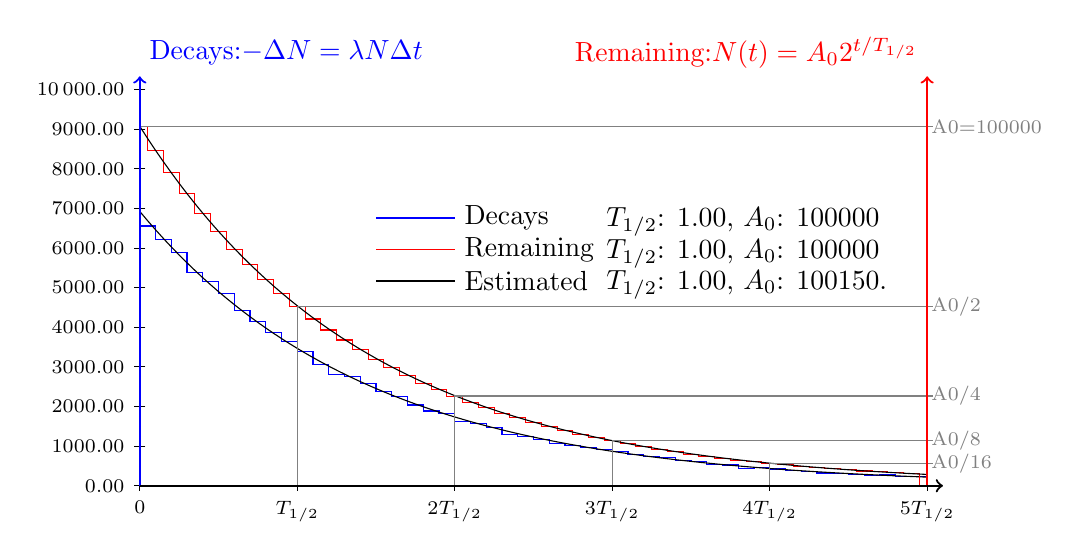
\begin{tikzpicture}[]
\begin{scope}[]
\clip (0.0,0.0) rectangle (10.0,5.0);
\begin{scope}[shift={(0.0,0.0)}]
\pgfsetxvec{\pgfpoint{2.0cm}{0cm}}
\pgfsetyvec{\pgfpoint{0cm}{0.0005cm}}
\begin{scope}[shift={(0.0,0.0)}]
\begin{scope}[draw=blue]
\pgfpathmoveto{ \pgfpointxy {5.0} {0.0}}
\pgfpathlineto{ \pgfpointxy {5.0} {230.0}}
\pgfpathlineto{ \pgfpointxy {4.9} {230.0}}
\pgfpathlineto{ \pgfpointxy {4.9} {244.0}}
\pgfpathlineto{ \pgfpointxy {4.8} {244.0}}
\pgfpathlineto{ \pgfpointxy {4.8} {271.0}}
\pgfpathlineto{ \pgfpointxy {4.7000003} {271.0}}
\pgfpathlineto{ \pgfpointxy {4.7000003} {264.0}}
\pgfpathlineto{ \pgfpointxy {4.6} {264.0}}
\pgfpathlineto{ \pgfpointxy {4.6} {290.0}}
\pgfpathlineto{ \pgfpointxy {4.5} {290.0}}
\pgfpathlineto{ \pgfpointxy {4.5} {306.0}}
\pgfpathlineto{ \pgfpointxy {4.4} {306.0}}
\pgfpathlineto{ \pgfpointxy {4.4} {322.0}}
\pgfpathlineto{ \pgfpointxy {4.3} {322.0}}
\pgfpathlineto{ \pgfpointxy {4.3} {365.0}}
\pgfpathlineto{ \pgfpointxy {4.2000003} {365.0}}
\pgfpathlineto{ \pgfpointxy {4.2000003} {394.0}}
\pgfpathlineto{ \pgfpointxy {4.1} {394.0}}
\pgfpathlineto{ \pgfpointxy {4.1} {423.0}}
\pgfpathlineto{ \pgfpointxy {4.0} {423.0}}
\pgfpathlineto{ \pgfpointxy {4.0} {457.0}}
\pgfpathlineto{ \pgfpointxy {3.9} {457.0}}
\pgfpathlineto{ \pgfpointxy {3.9} {443.0}}
\pgfpathlineto{ \pgfpointxy {3.8} {443.0}}
\pgfpathlineto{ \pgfpointxy {3.8} {525.0}}
\pgfpathlineto{ \pgfpointxy {3.7} {525.0}}
\pgfpathlineto{ \pgfpointxy {3.7} {536.0}}
\pgfpathlineto{ \pgfpointxy {3.6000001} {536.0}}
\pgfpathlineto{ \pgfpointxy {3.6000001} {613.0}}
\pgfpathlineto{ \pgfpointxy {3.5} {613.0}}
\pgfpathlineto{ \pgfpointxy {3.5} {630.0}}
\pgfpathlineto{ \pgfpointxy {3.4} {630.0}}
\pgfpathlineto{ \pgfpointxy {3.4} {714.0}}
\pgfpathlineto{ \pgfpointxy {3.3} {714.0}}
\pgfpathlineto{ \pgfpointxy {3.3} {730.0}}
\pgfpathlineto{ \pgfpointxy {3.2} {730.0}}
\pgfpathlineto{ \pgfpointxy {3.2} {785.0}}
\pgfpathlineto{ \pgfpointxy {3.1000001} {785.0}}
\pgfpathlineto{ \pgfpointxy {3.1000001} {864.0}}
\pgfpathlineto{ \pgfpointxy {3.0} {864.0}}
\pgfpathlineto{ \pgfpointxy {3.0} {910.0}}
\pgfpathlineto{ \pgfpointxy {2.9} {910.0}}
\pgfpathlineto{ \pgfpointxy {2.9} {965.0}}
\pgfpathlineto{ \pgfpointxy {2.8} {965.0}}
\pgfpathlineto{ \pgfpointxy {2.8} {1009.0}}
\pgfpathlineto{ \pgfpointxy {2.7} {1009.0}}
\pgfpathlineto{ \pgfpointxy {2.7} {1078.0}}
\pgfpathlineto{ \pgfpointxy {2.6000001} {1078.0}}
\pgfpathlineto{ \pgfpointxy {2.6000001} {1173.0}}
\pgfpathlineto{ \pgfpointxy {2.5} {1173.0}}
\pgfpathlineto{ \pgfpointxy {2.5} {1253.0}}
\pgfpathlineto{ \pgfpointxy {2.4} {1253.0}}
\pgfpathlineto{ \pgfpointxy {2.4} {1301.0}}
\pgfpathlineto{ \pgfpointxy {2.3} {1301.0}}
\pgfpathlineto{ \pgfpointxy {2.3} {1470.0}}
\pgfpathlineto{ \pgfpointxy {2.2} {1470.0}}
\pgfpathlineto{ \pgfpointxy {2.2} {1571.0}}
\pgfpathlineto{ \pgfpointxy {2.1000001} {1571.0}}
\pgfpathlineto{ \pgfpointxy {2.1000001} {1628.0}}
\pgfpathlineto{ \pgfpointxy {2.0} {1628.0}}
\pgfpathlineto{ \pgfpointxy {2.0} {1820.0}}
\pgfpathlineto{ \pgfpointxy {1.9} {1820.0}}
\pgfpathlineto{ \pgfpointxy {1.9} {1888.0}}
\pgfpathlineto{ \pgfpointxy {1.8000001} {1888.0}}
\pgfpathlineto{ \pgfpointxy {1.8000001} {2038.0}}
\pgfpathlineto{ \pgfpointxy {1.7} {2038.0}}
\pgfpathlineto{ \pgfpointxy {1.7} {2248.0}}
\pgfpathlineto{ \pgfpointxy {1.6} {2248.0}}
\pgfpathlineto{ \pgfpointxy {1.6} {2377.0}}
\pgfpathlineto{ \pgfpointxy {1.5} {2377.0}}
\pgfpathlineto{ \pgfpointxy {1.5} {2587.0}}
\pgfpathlineto{ \pgfpointxy {1.4} {2587.0}}
\pgfpathlineto{ \pgfpointxy {1.4} {2757.0}}
\pgfpathlineto{ \pgfpointxy {1.3000001} {2757.0}}
\pgfpathlineto{ \pgfpointxy {1.3000001} {2808.0}}
\pgfpathlineto{ \pgfpointxy {1.2} {2808.0}}
\pgfpathlineto{ \pgfpointxy {1.2} {3051.0}}
\pgfpathlineto{ \pgfpointxy {1.1} {3051.0}}
\pgfpathlineto{ \pgfpointxy {1.1} {3400.0}}
\pgfpathlineto{ \pgfpointxy {1.0} {3400.0}}
\pgfpathlineto{ \pgfpointxy {1.0} {3649.0}}
\pgfpathlineto{ \pgfpointxy {0.90000004} {3649.0}}
\pgfpathlineto{ \pgfpointxy {0.90000004} {3867.0}}
\pgfpathlineto{ \pgfpointxy {0.8} {3867.0}}
\pgfpathlineto{ \pgfpointxy {0.8} {4156.0}}
\pgfpathlineto{ \pgfpointxy {0.7} {4156.0}}
\pgfpathlineto{ \pgfpointxy {0.7} {4418.0}}
\pgfpathlineto{ \pgfpointxy {0.6} {4418.0}}
\pgfpathlineto{ \pgfpointxy {0.6} {4852.0}}
\pgfpathlineto{ \pgfpointxy {0.5} {4852.0}}
\pgfpathlineto{ \pgfpointxy {0.5} {5148.0}}
\pgfpathlineto{ \pgfpointxy {0.4} {5148.0}}
\pgfpathlineto{ \pgfpointxy {0.4} {5388.0}}
\pgfpathlineto{ \pgfpointxy {0.3} {5388.0}}
\pgfpathlineto{ \pgfpointxy {0.3} {5879.0}}
\pgfpathlineto{ \pgfpointxy {0.2} {5879.0}}
\pgfpathlineto{ \pgfpointxy {0.2} {6228.0}}
\pgfpathlineto{ \pgfpointxy {0.1} {6228.0}}
\pgfpathlineto{ \pgfpointxy {0.1} {6559.0}}
\pgfpathlineto{ \pgfpointxy {0.0} {6559.0}}
\pgfpathlineto{ \pgfpointxy {0.0} {0.0}}
\pgfusepath{ stroke, }
\end{scope}
\begin{scope}[black]
\pgfpathmoveto{ \pgfpointxy {0.0} {6926.170748444656}}
\pgfpathlineto{ \pgfpointxy {0.05} {6690.763194658762}}
\pgfpathlineto{ \pgfpointxy {0.1} {6463.356702121886}}
\pgfpathlineto{ \pgfpointxy {0.15} {6243.6793297680715}}
\pgfpathlineto{ \pgfpointxy {0.2} {6031.468379298172}}
\pgfpathlineto{ \pgfpointxy {0.25} {5826.470081035544}}
\pgfpathlineto{ \pgfpointxy {0.3} {5628.439290458907}}
\pgfpathlineto{ \pgfpointxy {0.35} {5437.139195049494}}
\pgfpathlineto{ \pgfpointxy {0.4} {5252.341031101914}}
\pgfpathlineto{ \pgfpointxy {0.45} {5073.823810160078}}
\pgfpathlineto{ \pgfpointxy {0.5} {4901.374054751056}}
\pgfpathlineto{ \pgfpointxy {0.55} {4734.785543100849}}
\pgfpathlineto{ \pgfpointxy {0.6} {4573.859062526792}}
\pgfpathlineto{ \pgfpointxy {0.65} {4418.402171211678}}
\pgfpathlineto{ \pgfpointxy {0.7} {4268.228968074752}}
\pgfpathlineto{ \pgfpointxy {0.75} {4123.159870464329}}
\pgfpathlineto{ \pgfpointxy {0.8} {3983.0213994062588}}
\pgfpathlineto{ \pgfpointxy {0.85} {3847.645972151357}}
\pgfpathlineto{ \pgfpointxy {0.9} {3716.87170177379}}
\pgfpathlineto{ \pgfpointxy {0.95} {3590.5422035807132}}
\pgfpathlineto{ \pgfpointxy {1.0} {3468.506408101695}}
\pgfpathlineto{ \pgfpointxy {1.05} {3350.618380434276}}
\pgfpathlineto{ \pgfpointxy {1.1} {3236.7371457296285}}
\pgfpathlineto{ \pgfpointxy {1.15} {3126.726520609644}}
\pgfpathlineto{ \pgfpointxy {1.2} {3020.4549503138232}}
\pgfpathlineto{ \pgfpointxy {1.25} {2917.7953513812467}}
\pgfpathlineto{ \pgfpointxy {1.3} {2818.624959679489}}
\pgfpathlineto{ \pgfpointxy {1.35} {2722.825183598743}}
\pgfpathlineto{ \pgfpointxy {1.4} {2630.2814622356013}}
\pgfpathlineto{ \pgfpointxy {1.45} {2540.8831283969052}}
\pgfpathlineto{ \pgfpointxy {1.5} {2454.523276259837}}
\pgfpathlineto{ \pgfpointxy {1.55} {2371.098633529997}}
\pgfpathlineto{ \pgfpointxy {1.6} {2290.509437944584}}
\pgfpathlineto{ \pgfpointxy {1.65} {2212.6593179730085}}
\pgfpathlineto{ \pgfpointxy {1.7} {2137.4551775722593}}
\pgfpathlineto{ \pgfpointxy {1.75} {2064.80708485923}}
\pgfpathlineto{ \pgfpointxy {1.8} {1994.6281645668525}}
\pgfpathlineto{ \pgfpointxy {1.85} {1926.8344941554537}}
\pgfpathlineto{ \pgfpointxy {1.9} {1861.3450034550874}}
\pgfpathlineto{ \pgfpointxy {1.95} {1798.0813777188384}}
\pgfpathlineto{ \pgfpointxy {2.0} {1736.967963971161}}
\pgfpathlineto{ \pgfpointxy {2.05} {1677.9316805392607}}
\pgfpathlineto{ \pgfpointxy {2.1} {1620.9019296593385}}
\pgfpathlineto{ \pgfpointxy {2.15} {1565.810513053182}}
\pgfpathlineto{ \pgfpointxy {2.2} {1512.5915503741492}}
\pgfpathlineto{ \pgfpointxy {2.25} {1461.181400425023}}
\pgfpathlineto{ \pgfpointxy {2.3} {1411.5185850535217}}
\pgfpathlineto{ \pgfpointxy {2.35} {1363.5437156344567}}
\pgfpathlineto{ \pgfpointxy {2.4} {1317.1994220506301}}
\pgfpathlineto{ \pgfpointxy {2.45} {1272.430284087526}}
\pgfpathlineto{ \pgfpointxy {2.5} {1229.182765159784}}
\pgfpathlineto{ \pgfpointxy {2.55} {1187.4051482901707}}
\pgfpathlineto{ \pgfpointxy {2.6} {1147.047474264514}}
\pgfpathlineto{ \pgfpointxy {2.65} {1108.0614818886354}}
\pgfpathlineto{ \pgfpointxy {2.7} {1070.4005502758316}}
\pgfpathlineto{ \pgfpointxy {2.75} {1034.0196430959022}}
\pgfpathlineto{ \pgfpointxy {2.8} {998.8752547190447}}
\pgfpathlineto{ \pgfpointxy {2.85} {964.9253581902192}}
\pgfpathlineto{ \pgfpointxy {2.9} {932.1293549717678}}
\pgfpathlineto{ \pgfpointxy {2.95} {900.4480263941834}}
\pgfpathlineto{ \pgfpointxy {3.0} {869.8434867569833}}
\pgfpathlineto{ \pgfpointxy {3.05} {840.2791380235891}}
\pgfpathlineto{ \pgfpointxy {3.1} {811.7196260560456}}
\pgfpathlineto{ \pgfpointxy {3.15} {784.1307983372425}}
\pgfpathlineto{ \pgfpointxy {3.2} {757.4796631300716}}
\pgfpathlineto{ \pgfpointxy {3.25} {731.7343500246944}}
\pgfpathlineto{ \pgfpointxy {3.3} {706.8640718267297}}
\pgfpathlineto{ \pgfpointxy {3.35} {682.8390877407925}}
\pgfpathlineto{ \pgfpointxy {3.4} {659.6306678053544}}
\pgfpathlineto{ \pgfpointxy {3.45} {637.2110585363964}}
\pgfpathlineto{ \pgfpointxy {3.5} {615.5534497387707}}
\pgfpathlineto{ \pgfpointxy {3.55} {594.6319424455797}}
\pgfpathlineto{ \pgfpointxy {3.6} {574.4215179472371}}
\pgfpathlineto{ \pgfpointxy {3.65} {554.8980078731744}}
\pgfpathlineto{ \pgfpointxy {3.7} {536.0380652904098}}
\pgfpathlineto{ \pgfpointxy {3.75} {517.8191367844275}}
\pgfpathlineto{ \pgfpointxy {3.8} {500.21943548897235}}
\pgfpathlineto{ \pgfpointxy {3.85} {483.21791503251205}}
\pgfpathlineto{ \pgfpointxy {3.9} {466.7942443702102}}
\pgfpathlineto{ \pgfpointxy {3.95} {450.9287834713141}}
\pgfpathlineto{ \pgfpointxy {4.0} {435.60255983288187}}
\pgfpathlineto{ \pgfpointxy {4.05} {420.7972457917633}}
\pgfpathlineto{ \pgfpointxy {4.1} {406.49513660770606}}
\pgfpathlineto{ \pgfpointxy {4.15} {392.6791292913727}}
\pgfpathlineto{ \pgfpointxy {4.2} {379.33270215195887}}
\pgfpathlineto{ \pgfpointxy {4.25} {366.4398950399428}}
\pgfpathlineto{ \pgfpointxy {4.3} {353.98529026135225}}
\pgfpathlineto{ \pgfpointxy {4.35} {341.9539941407178}}
\pgfpathlineto{ \pgfpointxy {4.4} {330.3316192106658}}
\pgfpathlineto{ \pgfpointxy {4.45} {319.1042670068554}}
\pgfpathlineto{ \pgfpointxy {4.5} {308.2585114476826}}
\pgfpathlineto{ \pgfpointxy {4.55} {297.78138277887587}}
\pgfpathlineto{ \pgfpointxy {4.6} {287.6603520637874}}
\pgfpathlineto{ \pgfpointxy {4.65} {277.8833162008277}}
\pgfpathlineto{ \pgfpointxy {4.7} {268.43858345013155}}
\pgfpathlineto{ \pgfpointxy {4.75} {259.31485945214376}}
\pgfpathlineto{ \pgfpointxy {4.8} {250.50123372140794}}
\pgfpathlineto{ \pgfpointxy {4.85} {241.9871665994058}}
\pgfpathlineto{ \pgfpointxy {4.9} {233.76247665084537}}
\pgfpathlineto{ \pgfpointxy {4.95} {225.81732848832505}}
\pgfpathlineto{ \pgfpointxy {5.0} {218.14222101081447}}
\pgfusepath{ stroke, }
\end{scope}
\end{scope}
\pgfsetxvec{\pgfpoint{1cm}{0cm}}
\pgfsetyvec{\pgfpoint{0cm}{1cm}}
\end{scope}
\end{scope}
\begin{scope}[shift={(0.0,0.0)}]
\pgfsetxvec{\pgfpoint{2.0cm}{0cm}}
\pgfsetyvec{\pgfpoint{0cm}{0.0005cm}}
\begin{scope}[shift={(0.0,0.0)}]
\begin{scope}[yshift=0cm]
\draw[black] [shift={(0.0,0.0)}] (0,2pt) -- (0,-2pt) node[below]{ \scriptsize{$0$}};
\draw[black] [shift={(1.0,0.0)}] (0,2pt) -- (0,-2pt) node[below]{ \scriptsize{$T_{1/2}$}};
\draw[black] [shift={(2.0,0.0)}] (0,2pt) -- (0,-2pt) node[below]{ \scriptsize{$2T_{1/2}$}};
\draw[black] [shift={(3.0,0.0)}] (0,2pt) -- (0,-2pt) node[below]{ \scriptsize{$3T_{1/2}$}};
\draw[black] [shift={(4.0,0.0)}] (0,2pt) -- (0,-2pt) node[below]{ \scriptsize{$4T_{1/2}$}};
\draw[black] [shift={(5.0,0.0)}] (0,2pt) -- (0,-2pt) node[below]{ \scriptsize{$5T_{1/2}$}};
\end{scope}
\begin{scope}[xshift=0cm]
\draw[black] [shift={(0.0,0.0)}] (2pt,0) -- (-2pt,0) node[left]{ \scriptsize{\num[round-mode=places,round-precision=2]{0}}};
\draw[black] [shift={(0.0,1000.0)}] (2pt,0) -- (-2pt,0) node[left]{ \scriptsize{\num[round-mode=places,round-precision=2]{1000}}};
\draw[black] [shift={(0.0,2000.0)}] (2pt,0) -- (-2pt,0) node[left]{ \scriptsize{\num[round-mode=places,round-precision=2]{2000}}};
\draw[black] [shift={(0.0,3000.0)}] (2pt,0) -- (-2pt,0) node[left]{ \scriptsize{\num[round-mode=places,round-precision=2]{3000}}};
\draw[black] [shift={(0.0,4000.0)}] (2pt,0) -- (-2pt,0) node[left]{ \scriptsize{\num[round-mode=places,round-precision=2]{4000}}};
\draw[black] [shift={(0.0,5000.0)}] (2pt,0) -- (-2pt,0) node[left]{ \scriptsize{\num[round-mode=places,round-precision=2]{5000}}};
\draw[black] [shift={(0.0,6000.0)}] (2pt,0) -- (-2pt,0) node[left]{ \scriptsize{\num[round-mode=places,round-precision=2]{6000}}};
\draw[black] [shift={(0.0,7000.0)}] (2pt,0) -- (-2pt,0) node[left]{ \scriptsize{\num[round-mode=places,round-precision=2]{7000}}};
\draw[black] [shift={(0.0,8000.0)}] (2pt,0) -- (-2pt,0) node[left]{ \scriptsize{\num[round-mode=places,round-precision=2]{8000}}};
\draw[black] [shift={(0.0,9000.0)}] (2pt,0) -- (-2pt,0) node[left]{ \scriptsize{\num[round-mode=places,round-precision=2]{9000}}};
\draw[black] [shift={(0.0,10000.0)}] (2pt,0) -- (-2pt,0) node[left]{ \scriptsize{\num[round-mode=places,round-precision=2]{10000}}};
\end{scope}
\end{scope}
\pgfsetxvec{\pgfpoint{1cm}{0cm}}
\pgfsetyvec{\pgfpoint{0cm}{1cm}}
\end{scope}
\begin{scope}[]
\clip (0.0,0.0) rectangle (10.0,5.0);
\begin{scope}[shift={(0.0,0.0)}]
\pgfsetxvec{\pgfpoint{2.0cm}{0cm}}
\pgfsetyvec{\pgfpoint{0cm}{0.00005cm}}
\begin{scope}[shift={(0.0,0.0)}]
\begin{scope}[draw=red]
\pgfpathmoveto{ \pgfpointxy {4.95} {0.0}}
\pgfpathlineto{ \pgfpointxy {4.95} {3348.0}}
\pgfpathlineto{ \pgfpointxy {4.85} {3348.0}}
\pgfpathlineto{ \pgfpointxy {4.85} {3592.0}}
\pgfpathlineto{ \pgfpointxy {4.75} {3592.0}}
\pgfpathlineto{ \pgfpointxy {4.75} {3863.0}}
\pgfpathlineto{ \pgfpointxy {4.65} {3863.0}}
\pgfpathlineto{ \pgfpointxy {4.65} {4127.0}}
\pgfpathlineto{ \pgfpointxy {4.5499997} {4127.0}}
\pgfpathlineto{ \pgfpointxy {4.5499997} {4417.0}}
\pgfpathlineto{ \pgfpointxy {4.45} {4417.0}}
\pgfpathlineto{ \pgfpointxy {4.45} {4723.0}}
\pgfpathlineto{ \pgfpointxy {4.35} {4723.0}}
\pgfpathlineto{ \pgfpointxy {4.35} {5045.0}}
\pgfpathlineto{ \pgfpointxy {4.25} {5045.0}}
\pgfpathlineto{ \pgfpointxy {4.25} {5410.0}}
\pgfpathlineto{ \pgfpointxy {4.15} {5410.0}}
\pgfpathlineto{ \pgfpointxy {4.15} {5804.0}}
\pgfpathlineto{ \pgfpointxy {4.0499997} {5804.0}}
\pgfpathlineto{ \pgfpointxy {4.0499997} {6227.0}}
\pgfpathlineto{ \pgfpointxy {3.95} {6227.0}}
\pgfpathlineto{ \pgfpointxy {3.95} {6684.0}}
\pgfpathlineto{ \pgfpointxy {3.8500001} {6684.0}}
\pgfpathlineto{ \pgfpointxy {3.8500001} {7127.0}}
\pgfpathlineto{ \pgfpointxy {3.75} {7127.0}}
\pgfpathlineto{ \pgfpointxy {3.75} {7652.0}}
\pgfpathlineto{ \pgfpointxy {3.65} {7652.0}}
\pgfpathlineto{ \pgfpointxy {3.65} {8188.0}}
\pgfpathlineto{ \pgfpointxy {3.5500002} {8188.0}}
\pgfpathlineto{ \pgfpointxy {3.5500002} {8801.0}}
\pgfpathlineto{ \pgfpointxy {3.45} {8801.0}}
\pgfpathlineto{ \pgfpointxy {3.45} {9431.0}}
\pgfpathlineto{ \pgfpointxy {3.3500001} {9431.0}}
\pgfpathlineto{ \pgfpointxy {3.3500001} {10145.0}}
\pgfpathlineto{ \pgfpointxy {3.25} {10145.0}}
\pgfpathlineto{ \pgfpointxy {3.25} {10875.0}}
\pgfpathlineto{ \pgfpointxy {3.15} {10875.0}}
\pgfpathlineto{ \pgfpointxy {3.15} {11660.0}}
\pgfpathlineto{ \pgfpointxy {3.0500002} {11660.0}}
\pgfpathlineto{ \pgfpointxy {3.0500002} {12524.0}}
\pgfpathlineto{ \pgfpointxy {2.95} {12524.0}}
\pgfpathlineto{ \pgfpointxy {2.95} {13434.0}}
\pgfpathlineto{ \pgfpointxy {2.8500001} {13434.0}}
\pgfpathlineto{ \pgfpointxy {2.8500001} {14399.0}}
\pgfpathlineto{ \pgfpointxy {2.75} {14399.0}}
\pgfpathlineto{ \pgfpointxy {2.75} {15408.0}}
\pgfpathlineto{ \pgfpointxy {2.65} {15408.0}}
\pgfpathlineto{ \pgfpointxy {2.65} {16486.0}}
\pgfpathlineto{ \pgfpointxy {2.5500002} {16486.0}}
\pgfpathlineto{ \pgfpointxy {2.5500002} {17659.0}}
\pgfpathlineto{ \pgfpointxy {2.45} {17659.0}}
\pgfpathlineto{ \pgfpointxy {2.45} {18912.0}}
\pgfpathlineto{ \pgfpointxy {2.3500001} {18912.0}}
\pgfpathlineto{ \pgfpointxy {2.3500001} {20213.0}}
\pgfpathlineto{ \pgfpointxy {2.25} {20213.0}}
\pgfpathlineto{ \pgfpointxy {2.25} {21683.0}}
\pgfpathlineto{ \pgfpointxy {2.15} {21683.0}}
\pgfpathlineto{ \pgfpointxy {2.15} {23254.0}}
\pgfpathlineto{ \pgfpointxy {2.0500002} {23254.0}}
\pgfpathlineto{ \pgfpointxy {2.0500002} {24882.0}}
\pgfpathlineto{ \pgfpointxy {1.95} {24882.0}}
\pgfpathlineto{ \pgfpointxy {1.95} {26702.0}}
\pgfpathlineto{ \pgfpointxy {1.85} {26702.0}}
\pgfpathlineto{ \pgfpointxy {1.85} {28590.0}}
\pgfpathlineto{ \pgfpointxy {1.7500001} {28590.0}}
\pgfpathlineto{ \pgfpointxy {1.7500001} {30628.0}}
\pgfpathlineto{ \pgfpointxy {1.6500001} {30628.0}}
\pgfpathlineto{ \pgfpointxy {1.6500001} {32876.0}}
\pgfpathlineto{ \pgfpointxy {1.5500001} {32876.0}}
\pgfpathlineto{ \pgfpointxy {1.5500001} {35253.0}}
\pgfpathlineto{ \pgfpointxy {1.45} {35253.0}}
\pgfpathlineto{ \pgfpointxy {1.45} {37840.0}}
\pgfpathlineto{ \pgfpointxy {1.35} {37840.0}}
\pgfpathlineto{ \pgfpointxy {1.35} {40597.0}}
\pgfpathlineto{ \pgfpointxy {1.2500001} {40597.0}}
\pgfpathlineto{ \pgfpointxy {1.2500001} {43405.0}}
\pgfpathlineto{ \pgfpointxy {1.1500001} {43405.0}}
\pgfpathlineto{ \pgfpointxy {1.1500001} {46456.0}}
\pgfpathlineto{ \pgfpointxy {1.0500001} {46456.0}}
\pgfpathlineto{ \pgfpointxy {1.0500001} {49856.0}}
\pgfpathlineto{ \pgfpointxy {0.95} {49856.0}}
\pgfpathlineto{ \pgfpointxy {0.95} {53505.0}}
\pgfpathlineto{ \pgfpointxy {0.85} {53505.0}}
\pgfpathlineto{ \pgfpointxy {0.85} {57372.0}}
\pgfpathlineto{ \pgfpointxy {0.75} {57372.0}}
\pgfpathlineto{ \pgfpointxy {0.75} {61528.0}}
\pgfpathlineto{ \pgfpointxy {0.65} {61528.0}}
\pgfpathlineto{ \pgfpointxy {0.65} {65946.0}}
\pgfpathlineto{ \pgfpointxy {0.55} {65946.0}}
\pgfpathlineto{ \pgfpointxy {0.55} {70798.0}}
\pgfpathlineto{ \pgfpointxy {0.45} {70798.0}}
\pgfpathlineto{ \pgfpointxy {0.45} {75946.0}}
\pgfpathlineto{ \pgfpointxy {0.35} {75946.0}}
\pgfpathlineto{ \pgfpointxy {0.35} {81334.0}}
\pgfpathlineto{ \pgfpointxy {0.25} {81334.0}}
\pgfpathlineto{ \pgfpointxy {0.25} {87213.0}}
\pgfpathlineto{ \pgfpointxy {0.15} {87213.0}}
\pgfpathlineto{ \pgfpointxy {0.15} {93441.0}}
\pgfpathlineto{ \pgfpointxy {0.05} {93441.0}}
\pgfpathlineto{ \pgfpointxy {0.05} {100000.0}}
\pgfpathlineto{ \pgfpointxy {-0.05} {100000.0}}
\pgfpathlineto{ \pgfpointxy {-0.05} {0.0}}
\pgfusepath{ stroke, }
\end{scope}
\begin{scope}[black]
\pgfpathmoveto{ \pgfpointxy {0.0} {100149.51712276821}}
\pgfpathlineto{ \pgfpointxy {0.05} {96745.62286503517}}
\pgfpathlineto{ \pgfpointxy {0.1} {93457.42058915786}}
\pgfpathlineto{ \pgfpointxy {0.15} {90280.978141652}}
\pgfpathlineto{ \pgfpointxy {0.2} {87212.4970155555}}
\pgfpathlineto{ \pgfpointxy {0.25} {84248.3078080339}}
\pgfpathlineto{ \pgfpointxy {0.3} {81384.86583237312}}
\pgfpathlineto{ \pgfpointxy {0.35} {78618.74687911248}}
\pgfpathlineto{ \pgfpointxy {0.4} {75946.64312124884}}
\pgfpathlineto{ \pgfpointxy {0.45} {73365.35915861506}}
\pgfpathlineto{ \pgfpointxy {0.5} {70871.80819670274}}
\pgfpathlineto{ \pgfpointxy {0.55} {68463.00835535962}}
\pgfpathlineto{ \pgfpointxy {0.6} {66136.0791029473}}
\pgfpathlineto{ \pgfpointxy {0.65} {63888.23781169537}}
\pgfpathlineto{ \pgfpointxy {0.7} {61716.796430132556}}
\pgfpathlineto{ \pgfpointxy {0.75} {59619.15826861566}}
\pgfpathlineto{ \pgfpointxy {0.8} {57592.814894112445}}
\pgfpathlineto{ \pgfpointxy {0.85} {55635.34313052484}}
\pgfpathlineto{ \pgfpointxy {0.9} {53744.40216096576}}
\pgfpathlineto{ \pgfpointxy {0.95} {51917.730728523915}}
\pgfpathlineto{ \pgfpointxy {1.0} {50153.14443216944}}
\pgfpathlineto{ \pgfpointxy {1.05} {48448.53311456674}}
\pgfpathlineto{ \pgfpointxy {1.1} {46801.858338670376}}
\pgfpathlineto{ \pgfpointxy {1.15} {45211.15095008709}}
\pgfpathlineto{ \pgfpointxy {1.2} {43674.50872228831}}
\pgfpathlineto{ \pgfpointxy {1.25} {42190.09408185753}}
\pgfpathlineto{ \pgfpointxy {1.3} {40756.13191105239}}
\pgfpathlineto{ \pgfpointxy {1.35} {39370.90742505332}}
\pgfpathlineto{ \pgfpointxy {1.4} {38032.764121360735}}
\pgfpathlineto{ \pgfpointxy {1.45} {36740.10179888826}}
\pgfpathlineto{ \pgfpointxy {1.5} {35491.37464438326}}
\pgfpathlineto{ \pgfpointxy {1.55} {34285.08938388645}}
\pgfpathlineto{ \pgfpointxy {1.6} {33119.80349701976}}
\pgfpathlineto{ \pgfpointxy {1.65} {31994.123491967377}}
\pgfpathlineto{ \pgfpointxy {1.7} {30906.703239086783}}
\pgfpathlineto{ \pgfpointxy {1.75} {29856.242361157398}}
\pgfpathlineto{ \pgfpointxy {1.8} {28841.484678341516}}
\pgfpathlineto{ \pgfpointxy {1.85} {27861.216705998162}}
\pgfpathlineto{ \pgfpointxy {1.9} {26914.266203553427}}
\pgfpathlineto{ \pgfpointxy {1.95} {25999.500772691987}}
\pgfpathlineto{ \pgfpointxy {2.0} {25115.826503193468}}
\pgfpathlineto{ \pgfpointxy {2.05} {24262.186664794248}}
\pgfpathlineto{ \pgfpointxy {2.1} {23437.560443510498}}
\pgfpathlineto{ \pgfpointxy {2.15} {22640.961720911168}}
\pgfpathlineto{ \pgfpointxy {2.2} {21871.437894881234}}
\pgfpathlineto{ \pgfpointxy {2.25} {21128.068740464954}}
\pgfpathlineto{ \pgfpointxy {2.3} {20409.965309426967}}
\pgfpathlineto{ \pgfpointxy {2.35} {19716.268867215207}}
\pgfpathlineto{ \pgfpointxy {2.4} {19046.14986605453}}
\pgfpathlineto{ \pgfpointxy {2.45} {18398.806952942792}}
\pgfpathlineto{ \pgfpointxy {2.5} {17773.466011363525}}
\pgfpathlineto{ \pgfpointxy {2.55} {17169.379235568784}}
\pgfpathlineto{ \pgfpointxy {2.6} {16585.824236325483}}
\pgfpathlineto{ \pgfpointxy {2.65} {16022.103177055762}}
\pgfpathlineto{ \pgfpointxy {2.7} {15477.541939338244}}
\pgfpathlineto{ \pgfpointxy {2.75} {14951.489316772395}}
\pgfpathlineto{ \pgfpointxy {2.8} {14443.316236241903}}
\pgfpathlineto{ \pgfpointxy {2.85} {13952.415005645857}}
\pgfpathlineto{ \pgfpointxy {2.9} {13478.198587198156}}
\pgfpathlineto{ \pgfpointxy {2.95} {13020.099895426034}}
\pgfpathlineto{ \pgfpointxy {3.0} {12577.571119028411}}
\pgfpathlineto{ \pgfpointxy {3.05} {12150.08306578291}}
\pgfpathlineto{ \pgfpointxy {3.1} {11737.124529718276}}
\pgfpathlineto{ \pgfpointxy {3.15} {11338.20167979549}}
\pgfpathlineto{ \pgfpointxy {3.2} {10952.83746936635}}
\pgfpathlineto{ \pgfpointxy {3.25} {10580.571065703547}}
\pgfpathlineto{ \pgfpointxy {3.3} {10220.957298919873}}
\pgfpathlineto{ \pgfpointxy {3.35} {9873.566129617686}}
\pgfpathlineto{ \pgfpointxy {3.4} {9537.982134631926}}
\pgfpathlineto{ \pgfpointxy {3.45} {9213.804010251803}}
\pgfpathlineto{ \pgfpointxy {3.5} {8900.644092327007}}
\pgfpathlineto{ \pgfpointxy {3.55} {8598.12789268465}}
\pgfpathlineto{ \pgfpointxy {3.6} {8305.89365130247}}
\pgfpathlineto{ \pgfpointxy {3.65} {8023.591903702907}}
\pgfpathlineto{ \pgfpointxy {3.7} {7750.885063050566}}
\pgfpathlineto{ \pgfpointxy {3.75} {7487.447016453448}}
\pgfpathlineto{ \pgfpointxy {3.8} {7232.9627349851335}}
\pgfpathlineto{ \pgfpointxy {3.85} {6987.12789696158}}
\pgfpathlineto{ \pgfpointxy {3.9} {6749.648524022027}}
\pgfpathlineto{ \pgfpointxy {3.95} {6520.240629578851}}
\pgfpathlineto{ \pgfpointxy {4.0} {6298.62987921593}}
\pgfpathlineto{ \pgfpointxy {4.05} {6084.551262629423}}
\pgfpathlineto{ \pgfpointxy {4.1} {5877.748776718706}}
\pgfpathlineto{ \pgfpointxy {4.15} {5677.975119448398}}
\pgfpathlineto{ \pgfpointxy {4.2} {5484.991394115514}}
\pgfpathlineto{ \pgfpointxy {4.25} {5298.566823667932}}
\pgfpathlineto{ \pgfpointxy {4.3} {5118.4784747327185}}
\pgfpathlineto{ \pgfpointxy {4.35} {4944.510991024184}}
\pgfpathlineto{ \pgfpointxy {4.4} {4776.456335812881}}
\pgfpathlineto{ \pgfpointxy {4.45} {4614.113543147633}}
\pgfpathlineto{ \pgfpointxy {4.5} {4457.288477533037}}
\pgfpathlineto{ \pgfpointxy {4.55} {4305.793601775066}}
\pgfpathlineto{ \pgfpointxy {4.6} {4159.447752717211}}
\pgfpathlineto{ \pgfpointxy {4.65} {4018.0759245988706}}
\pgfpathlineto{ \pgfpointxy {4.7} {3881.509059777031}}
\pgfpathlineto{ \pgfpointxy {4.75} {3749.5838465609004}}
\pgfpathlineto{ \pgfpointxy {4.8} {3622.142523917763}}
\pgfpathlineto{ \pgfpointxy {4.85} {3499.032692816526}}
\pgfpathlineto{ \pgfpointxy {4.9} {3380.1071339833443}}
\pgfpathlineto{ \pgfpointxy {4.95} {3265.2236318513847}}
\pgfpathlineto{ \pgfpointxy {5.0} {3154.2448044941984}}
\pgfusepath{ stroke, }
\end{scope}
\end{scope}
\pgfsetxvec{\pgfpoint{1cm}{0cm}}
\pgfsetyvec{\pgfpoint{0cm}{1cm}}
\end{scope}
\end{scope}
\begin{scope}[shift={(0.0,0.0)}]
\pgfsetxvec{\pgfpoint{2.0cm}{0cm}}
\pgfsetyvec{\pgfpoint{0cm}{0.00005cm}}
\begin{scope}[shift={(0.0,0.0)}]
\begin{scope}[gray]
\pgfpathmoveto{ \pgfpointxy {0.0} {0.0}}
\pgfpathlineto{ \pgfpointxy {0.0} {100000.0}}
\pgfpathlineto{ \pgfpointxy {5.0} {100000.0}}
\pgfusepath{ stroke, }
\end{scope}
\begin{scope}[gray]
\pgfpathmoveto{ \pgfpointxy {1.0} {0.0}}
\pgfpathlineto{ \pgfpointxy {1.0} {50000.0}}
\pgfpathlineto{ \pgfpointxy {5.0} {50000.0}}
\pgfusepath{ stroke, }
\end{scope}
\begin{scope}[gray]
\pgfpathmoveto{ \pgfpointxy {2.0} {0.0}}
\pgfpathlineto{ \pgfpointxy {2.0} {25000.0}}
\pgfpathlineto{ \pgfpointxy {5.0} {25000.0}}
\pgfusepath{ stroke, }
\end{scope}
\begin{scope}[gray]
\pgfpathmoveto{ \pgfpointxy {3.0} {0.0}}
\pgfpathlineto{ \pgfpointxy {3.0} {12500.0}}
\pgfpathlineto{ \pgfpointxy {5.0} {12500.0}}
\pgfusepath{ stroke, }
\end{scope}
\begin{scope}[gray]
\pgfpathmoveto{ \pgfpointxy {4.0} {0.0}}
\pgfpathlineto{ \pgfpointxy {4.0} {6250.0}}
\pgfpathlineto{ \pgfpointxy {5.0} {6250.0}}
\pgfusepath{ stroke, }
\end{scope}
\begin{scope}[xshift=10cm]
\draw[gray] [shift={(0.0,100000.0)}] (2pt,0) -- (-2pt,0) node[right]{ \scriptsize{A0=100000}};
\draw[gray] [shift={(0.0,50000.0)}] (2pt,0) -- (-2pt,0) node[right]{ \scriptsize{A0/2}};
\draw[gray] [shift={(0.0,25000.0)}] (2pt,0) -- (-2pt,0) node[right]{ \scriptsize{A0/4}};
\draw[gray] [shift={(0.0,12500.0)}] (2pt,0) -- (-2pt,0) node[right]{ \scriptsize{A0/8}};
\draw[gray] [shift={(0.0,6250.0)}] (2pt,0) -- (-2pt,0) node[right]{ \scriptsize{A0/16}};
\end{scope}
\end{scope}
\pgfsetxvec{\pgfpoint{1cm}{0cm}}
\pgfsetyvec{\pgfpoint{0cm}{1cm}}
\end{scope}
\node[right,blue] at (0.0,5.5) {Decays:$-\Delta N = \lambda N \Delta t$};
\node[left,red] at (10.0,5.5) {Remaining:$N(t) = A_0 2^{t/T_{1/2}}$};
\draw[blue,thick,->] (0.0,0.0) -- (0.0,5.2);
\draw[red,thick,->] (10.0,0.0) -- (10.0,5.2);
\draw[black,thick,->] (0.0,0.0) -- (10.2,0.0);
\draw[blue] (3.0,3.4) -- (4.0,3.4);
\node[right,] at (4.0,3.4) {Decays};
\node[right] at (5.8,3.35) {$T_{1/2}$: 1.00, $A_0$: 100000};
\draw[red] (3.0,3.0) -- (4.0,3.0);
\node[right,] at (4.0,3.0) {Remaining};
\node[right] at (5.8,2.95) {$T_{1/2}$: 1.00, $A_0$: 100000};
\draw[black] (3.0,2.6) -- (4.0,2.6);
\node[right,] at (4.0,2.6) {Estimated};
\node[right] at (5.8,2.55) {$T_{1/2}$:  1.00, $A_0$: 100150.};
\end{tikzpicture}
%%% Local Variables: 
%%% mode: latex 
%%% TeX-master: "master" 
%%% End:


  \caption{ Two different axes in plot. The red histogram is the simulated number of
    remaining nuclei, the blue is the number of decays per time interval. The half-life and
    the number of nuclei at time=0 is estimated by a levmar fit to the number if decays.}
\end{figure}

\end{document}
  
%%% Local Variables: 
%%% mode: latex
%%% TeX-master: t
%%% End: 
